%%%%%%%%%%%%%%%%%%%%%%%%%%%%%%%%%%%%%%%%%
% Masters/Doctoral Thesis 
% LaTeX Template
% Version 1.43 (17/5/14)
%
% This template has been downloaded from:
% http://www.LaTeXTemplates.com
%
% Original authors:
% Steven Gunn 
% http://users.ecs.soton.ac.uk/srg/softwaretools/document/templates/
% and
% Sunil Patel
% http://www.sunilpatel.co.uk/thesis-template/
%
% License:
% CC BY-NC-SA 3.0 (http://creativecommons.org/licenses/by-nc-sa/3.0/)
%
% Note:
% Make sure to edit document variables in the Thesis.cls file
%
%%%%%%%%%%%%%%%%%%%%%%%%%%%%%%%%%%%%%%%%%

%----------------------------------------------------------------------------------------
%	PACKAGES AND OTHER DOCUMENT CONFIGURATIONS
%----------------------------------------------------------------------------------------

\documentclass[11pt, twoside]{Thesis} 
\graphicspath{{Pictures/}} % Specifies the directory where pictures are stored

\usepackage[backend=biber, sorting=none, bibstyle=numeric, citestyle=numeric-comp, giveninits=true]{biblatex}
\renewbibmacro{in:}{%
  \ifentrytype{article}{}{\printtext{\bibstring{in}\intitlepunct}}}

  
\bibliography{Bibliography}
\usepackage{csquotes}
\usepackage{bookmark}
\usepackage{diagbox}

\usepackage{xpatch}
\makeatletter
\xpatchcmd{\@endpart}{\vfil\newpage}{}{}{}
\xpatchcmd{\@endpart}{\newpage}{}{}{}
\makeatother

\usepackage{dblfloatfix}
\usepackage{float}
\usepackage{color}

%%%%TIKZ:
\usepackage{pgfplots}
\usetikzlibrary{calc}
\usetikzlibrary{arrows}
\usetikzlibrary{shapes.misc}
\tikzset{cross/.style={cross out, draw=black, minimum size=2*(#1-\pgflinewidth), inner sep=0pt, outer sep=0pt}, cross/.default={3pt}}
\pgfplotsset{compat=1.13}

%\usepackage[square, numbers, comma, sort&compress]{natbib} % Use the natbib reference package - read up on this to edit the reference style; if you want text (e.g. Smith et al., 2012) for the in-text references (instead of numbers), remove 'numbers' 
%[activate={true,nocompatibility},final,tracking=true,kerning=true,spacing=true,factor=1100,stretch=10,shrink=10]
\usepackage{microtype}
\microtypecontext{spacing=nonfrench}

\hypersetup{urlcolor=red, linkcolor=black, colorlinks=false} % Colors hyperlinks in blue - change to black if annoying

\usepackage{caption}
\captionsetup{
  font=footnotesize,
  justification=raggedright,
  singlelinecheck=false
}

\title{\ttitle} % Defines the thesis title - don't touch this



\begin{document}

\frontmatter % Use roman page numbering style (i, ii, iii, iv...) for the pre-content pages

\setstretch{1.3} % Line spacing of 1.3

% Define the page headers using the FancyHdr package and set up for one-sided printing
\fancyhead{} % Clears all page headers and footers
\fancyhead[LE,RO]{\thepage} %alternates page number left even, right odd.
% \rhead{\thepage} % Sets the right side header to show the page number
\lhead{} % Clears the left side page header

\pagestyle{fancy} % Finally, use the "fancy" page style to implement the FancyHdr headers

\newcommand{\HRule}{\rule{\linewidth}{0.5mm}} % New command to make the lines in the title page

% PDF meta-data
\hypersetup{pdftitle={\ttitle}}
\hypersetup{pdfsubject=\subjectname}
\hypersetup{pdfauthor=\authornames}
\hypersetup{pdfkeywords=\keywordnames}

%----------------------------------------------------------------------------------------
%	TITLE PAGE
%----------------------------------------------------------------------------------------

\begin{titlepage}
\begin{center}

\textsc{\LARGE \univname}\\[1.5cm] % University name
\textsc{\Large Master's Thesis}\\[0.5cm] % Thesis type

\HRule \\[0.4cm] % Horizontal line
{\huge \bfseries \ttitle}\\[0.4cm] % Thesis title
\HRule \\[1.5cm] % Horizontal line
 
\begin{minipage}[t]{0.4\textwidth}
\begin{flushleft} \large
\emph{Author:}\\
{\authornames}\\ 
{Student ID: 201205966} % Author name - remove the \href bracket to remove the link 
\end{flushleft}
\end{minipage}%
\begin{minipage}[t]{0.4\textwidth}
\begin{flushright} \large
\emph{Supervisor:} \\
{\supname} % Supervisor name - remove the \href bracket to remove the link  
\end{flushright}
\end{minipage}\\[0cm]
\vspace{2.5cm}
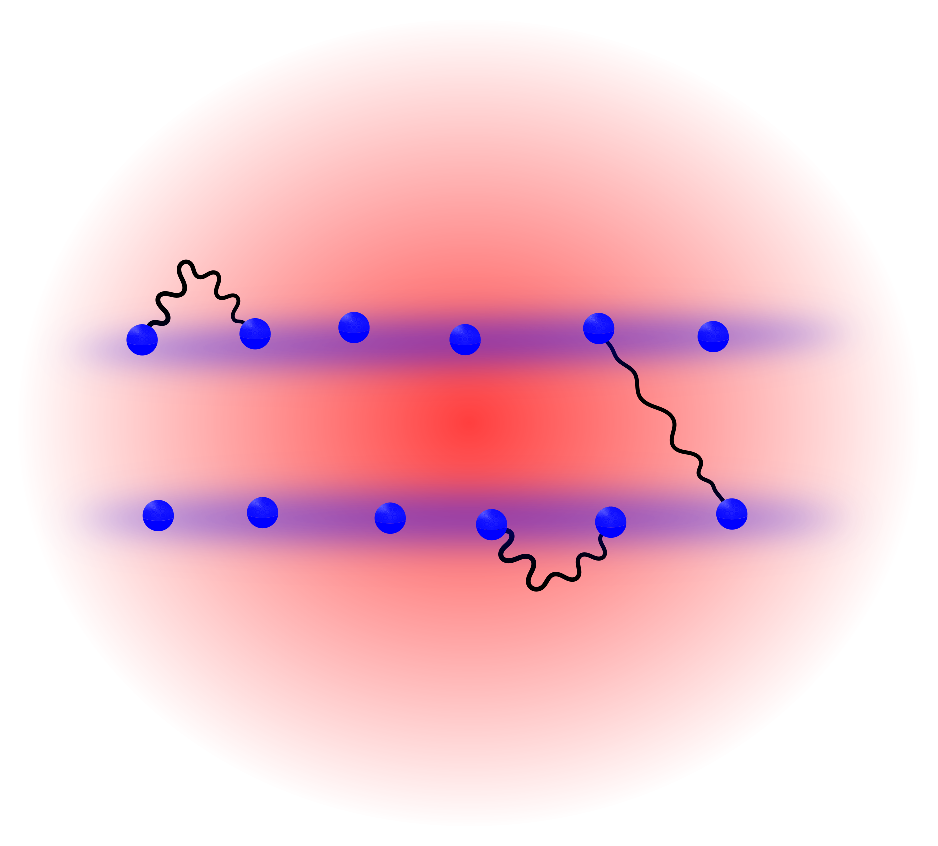
\includegraphics[width=0.6\columnwidth]{1D3Dsketchfrontpage.eps} 
 
\large 
\deptname \\ \facname \\[1cm] % Research group name and department name


 
{\large June 16, 2017} % Date

 
\vfill
\end{center}

\end{titlepage}


%----------------------------------------------------------------------------------------
%	DECLARATION PAGE
%	Your institution may give you a different text to place here
%----------------------------------------------------------------------------------------

%\Declaration{

%\addtocontents{toc}{\vspace{1em}} % Add a gap in the Contents, for aesthetics

%, \authornames, declare that this thesis titled, '\ttitle' and the work presented in it are my own. I confirm that:

%\begin{itemize} 
%\item[\tiny{$\blacksquare$}] This work was done wholly or mainly while in candidature for a research degree at this University.
%\item[\tiny{$\blacksquare$}] Where any part of this thesis has previously been submitted for a degree or any other qualification at this University or any other institution, this has been clearly stated.
%\item[\tiny{$\blacksquare$}] Where I have consulted the published work of others, this is always clearly attributed.
%\item[\tiny{$\blacksquare$}] Where I have quoted from the work of others, the source is always given. With the exception of such quotations, this thesis is entirely my own work.
%\item[\tiny{$\blacksquare$}] I have acknowledged all main sources of help.
%\item[\tiny{$\blacksquare$}] Where the thesis is based on work done by myself jointly with others, I have made clear exactly what was done by others and what I have contributed myself.\\
%\end{itemize}
 
%Signed:\\
%\rule[1em]{25em}{0.5pt} % This prints a line for the signature
 
%Date:\\
%\rule[1em]{25em}{0.5pt} % This prints a line to write the date
%}

%\clearpage % Start a new page

%----------------------------------------------------------------------------------------
%	QUOTATION PAGE
%----------------------------------------------------------------------------------------

%\pagestyle{empty} % No headers or footers for the following pages

%\null\vfill % Add some space to move the quote down the page a bit

%\textit{``Thanks to my solid academic training, today I can write hundreds of words on virtually any topic without possessing a shred of information, which is how I got a good job in journalism."}

%\begin{flushright}
%Dave Barry
%\end{flushright}

%\vfill\vfill\vfill\vfill\vfill\vfill\null % Add some space at the bottom to position the quote just right

%\clearpage % Start a new page

%----------------------------------------------------------------------------------------
%	ABSTRACT PAGE
%----------------------------------------------------------------------------------------

\cleardoublepage

\setstretch{1.3} % Reset the line-spacing to 1.3 for body text (if it has changed)

\addtotoc{Summary} % Add the "Abstract" page entry to the Contents

\abstract{\addtocontents{toc}{\vspace{1em}} % Add a gap in the Contents, for aesthetics

In this thesis we theoretically investigate the properties of Fermi-Bose mixtures, both in a 1D-3D mixed dimensional setup and in a pure 1D setup. First, we investigate two one-dimensional wires of gas constituted by identical fermions embedded in a three-dimensional Bose-Einstein condensate of identical bosons. The fermions and bosons are assumed to interact through a point interaction. The surrounding condensate hereby induces an attractive interaction between the fermions. As a result, the fermions form a superfluid. This double wire system is then studied in a weak coupling limit in a mean field approach. The intra- and interwire interactions then respectively result in $p$- and $s$-wave pairing of the fermions. Hence, a system of interacting Kitaev wires is realised. We can control a $p$- to $s$-wave phase transition by adjusting the interwire distance. The separated wires with $p$-wave pairing are shown to have a topological ground state. In turn a single edge state emerge in each wire. As the interwire distance decreases the $s$-wave pairing becomes dominant and the system becomes topologically trivial. In turn the edge states vanish. We show that for the energetically favourable transition the edge states couple and in turn gradually gap away. Thus the bulk gap remains open. The phase transition is second order. 

Second, in the pure one-dimensional setup we investigate a Kitaev model of fermions in a 1D lattice with both nearest and next-nearest neighbour hopping. This is embedded within a 1D Bose gas. For a high filling fraction and long interaction range we show that it is possible to find phases with winding numbers larger than 1. As a result, several edge states emerge.  
}

%----------------------------------------------------------------------------------------
%	ACKNOWLEDGEMENTS
%----------------------------------------------------------------------------------------
\cleardoublepage

\setstretch{1.3} % Reset the line-spacing to 1.3 for body text (if it has changed)

\preface{\addtocontents{toc}{\vspace{1em}} % Add a gap in the Contents, for aesthetics
The thesis is organised in the following way. Part I is introductory. We motivate the present work and come with a short summary of the most important ingredients of condensed matter physics for understanding the system at hand. In part II, chapters \ref{Chapter3} through \ref{Chapter6}, we investigate the double wire system. In part III, chapters \ref{Chapter7} and \ref{Chapter8}, we investigate the extended Kitaev chain supporting several edge states. In part IV we come with our conclusions. Finally, the supplementary material is listed in part V, appendices \ref{Appendix.intrawireinteraction.ltnonzero} to \ref{Appendix.groundstatedepletion.1DBosegas}. 

I would like to thank my supervisor, associate professor Georg Bruun, for his guidance and faith in me as a student. Throughout our collaboration he has been nothing but inspiring, enthusiastic and supportive. Further, I thank PhD student Jonatan Midtgaard for many frustrating but also interesting and illuminating discussions about the systems we both study. I also thank him for helping with illustrating the double wire system. I thank postdoc Zhigang Wu for his comments and thoughts, especially on the one-dimensional Bose gas. Finally, I would like to thank my love, Nana, for being ever so patient and interested.   
}
\clearpage
%----------------------------------------------------------------------------------------
%	ABBREVIATIONS
%----------------------------------------------------------------------------------------

%\setstretch{1.5} % Set the line spacing to 1.5, this makes the following tables easier to read

%\lhead{\emph{Abbreviations}} % Set the left side page header to "Abbreviations"
%\listofsymbols{ll} % Include a list of Abbreviations (a table of two columns)
%{
%\textbf{B} & \textbf{B}osons \\
%\textbf{BCS} & \textbf{B}ardeen-\textbf{C}ooper-\textbf{S}chrieffer \\
%\textbf{BdG} & \textbf{B}ogoliubov-\textbf{d}e \textbf{G}ennes \\
%\textbf{BEC} & \textbf{B}ose-\textbf{E}instein \textbf{C}ondensate \\
%\textbf{F} & \textbf{F}ermions \\
%}
%\clearpage
%----------------------------------------------------------------------------------------
%	SYMBOLS
%----------------------------------------------------------------------------------------
%\setstretch{1.5} % Set the line spacing to 1.5, this makes the following tables easier to read

%\lhead{\emph{Symbols}} % Set the left side page header to "Symbols"

%\listofnomenclature{ll} % Include a list of Symbols (a three column table)
%{
%$\beta$ & inverse temperature: $\beta = 1/k_BT$ \\
%$\mathcal{L}$ & length of fermionic wires \\ \\

%$H$ & Hamiltonian, second quantization \\
%$\mathcal{H}$ & Hamiltonian, first quantization \\
%$b_k$ & annihilation operator for real boson \\
%$\beta_k$ & annihilation operator for corresponding boson quasiparticle \\
%$c_k$ & annihilation operator for real fermion \\
%$\gamma_k$ & annihilation operator for corresponding fermion quasiparticle \\ \\

%$m_B$ & mass of bosons \\
%$m_F$ & mass of fermions \\
%$m_r$ & reduced mass: $m_r = \frac{m_Fm_B}{m_F + m_B}$ \\ \\

%$\epsilon_{F,0}$ & Fermi energy, free gas \\
%$k_F$ & Fermi momentum, free gas: $\epsilon_{F,0} = \frac{k_F^2}{2m_F}$ \\
%$T_F$ & Fermi temperature, free gas: $\epsilon_{F,0} = k_BT_F$ \\
%$\mu$ & chemical potential of fermions \\ \\

%$n_F$ & density of fermions: $k_F = \pi n_F$ \\
%$n_B$ & density of bosons \\ \\

%$E_{F,k}$ & energy dispersion of fermion quasiparticles  \\
%$E_{B,k}$ & energy dispersion of boson quasiparticles \\ \\

%$g_B$ & point interaction strength between bosons \\
%$g_{BF}$ & point interaction strength between bosons and fermions \\
%$a_B$ & BEC scattering length: $g_B = \frac{4\pi a_B}{m_B}$ \\
%$a_{BF}$ & Bose-Fermi scattering length: $g_B = \frac{2\pi a_{BF}}{m_r}$ \\ \\

%$v_F$ & speed of fermions, free gas: $k_F = m_Fv_F$ \\
%$c_0$ & speed of bosons: $c_0 = \sqrt{\frac{n_Bg_B}{m_B}}$ \\
%$\xi$ & BEC coherence length: $\xi = \frac{1}{\sqrt{2m_Bn_Bg_B}}$ \\ \\

%$\omega_t$ & trapping frequency, fermion wires \\
%$l_t$ & trapping width, fermion wires: $l_t = \frac{1}{m_F\omega^2_t}$ \\ \\

%$f(E)$ & Fermi-Dirac distribution function \\
%$b(E)$ & Bose-Einstein distribution function \\
%$\omega_n$ & Matsubara frequency. Bosonic: $\omega_n = \frac{2\pi n}{\beta}$. Fermionic: $\omega_n = \frac{2\pi (n+1)}{\beta}$  \\ \\

%$\chi_{\text{BEC}}$ & BEC density-density correlation function \\
%$d$ & interwire distance \\
%$V^{ij}_{\text{ind}}$ & induced interaction between wires $i$ and $j$ in momentum space  \\
%$\tilde{V}^{ij}_{\text{ind}}$ & induced interaction between wires $i$ and $j$ in real space  \\
%$\Delta^{ij}_k$ & pairing potential between wires $i$ and $j$ in momentum space \\ \\

%$\ket{\text{BEC}}_0$ & BEC bosonic ground state at zero temperature	\\
%$\ket{\text{S}}_0$ & BCS fermionic superfluid ground state at zero temperature \\
%$T_c$ & critical temperature between superfluid and normal phase \\ \\

%$T$ & time reversal transformation, second quantization \\
%$C$ & particle-hole transformation, second quantization \\
%$S$ & chiral transformation, second quantization \\ \\

%$\mathcal{T}$ & time reversal transformation, first quantization \\
%$\mathcal{C}$ & particle-hole transformation, first quantization \\
%$\mathcal{S}$ & chiral transformation, first quantization \\ \\

%$\mathcal{A}$ & Berry connection \\
%$\text{CS}_1$ & Chern-Simons invariant in one dimension
%}
%\newpage

%----------------------------------------------------------------------------------------
%	LIST OF CONTENTS/FIGURES/TABLES PAGES
%----------------------------------------------------------------------------------------

\setstretch{1.3}

%\pagestyle{fancy} % The page style headers have been "empty" all this time, now use the "fancy" headers as defined before to bring them back

\fancyhead[LE,RO]{\thepage}
\fancyhead[LO,RE]{\emph{Contents}} % Set the left side page header to "Contents"
\tableofcontents % Write out the Table of Contents

%\lhead{\emph{List of figures}} % Set the left side page header to "List of Figures"
%\listoffigures % Write out the List of Figures and Tables

%\lhead{\emph{List of tables}} % Set the left side page header to "List of Tables"
%\listoftables % Write out the List of Tables

%----------------------------------------------------------------------------------------
%	THESIS CONTENT - CHAPTERS
%----------------------------------------------------------------------------------------

\mainmatter % Begin numeric (1,2,3...) page numbering

\pagestyle{fancy} % Return the page headers back to the "fancy" style
\fancyhead[LE,RO]{\thepage}

% Include the chapters of the thesis as separate files from the Chapters folder
% Uncomment the lines as you write the chapters


\part{Introductions}
\newpage

% Chapter 1

\chapter{Introduction} % Main chapter title

\label{Chapter1} % For referencing the chapter elsewhere, use \ref{Chapter1} 

\lhead{Part I. \emph{Introductions}}
\chead{Chapter 1. \emph{Introduction}} % This is for the header on each page - perhaps a shortened title

%----------------------------------------------------------------------------------------

This thesis is a study of how one can theoretically realise a topological superfluid in mixtures of fermions and bosons. Specifically, we look at fermion wires immersed in a sea of bosons, a 1D-3D Fermi-Bose mixture. We investigate how a point interaction between the fermions and bosons induce an attractive interaction between the fermions themselves. Using a mean field approach in a weak coupling limit this leads to the realisation of the socalled Kitaev model for spinless $p$-wave superfluids. The system is characterized by having a topological phase as its ground state. 

The study of topological phases of matter is in a thriving development, being one of the biggest research areas of modern condensed matter physics and receiving the 2016 Nobel Prize in Physics \cite{NobelPrize2016}. The reason for this development is in part, that topological phases of matter gives a whole new perspective on condensed matter physics, revealing up to now unknown states of matter. Therefore, it is of high interest to realise simple yet tunable topological phases of matter. The specific 1D-3D Fermi-Bose mixture is in this sense a well suited candidate for investigation. Firstly, an analogous 2D-3D mixture has been experimentally realised, and so it is reasonable to believe that this system can as well. (INSERT REFERENCE) Secondly, just like the 2D-3D mixture there is a high degree of tunability through several system parameters. 

The thesis is organised in the following way. In chapter \ref{Chapter2} we come with a short summary of the most important ingredients of condensed matter physics for understanding the system at hand. In part II, chapters \ref{Chapter3} through \ref{Chapter7}, we investigate the \textit{single} fermion wire system. The focus is on the bulk properties of the system, specifically how the superfluidity of the fermion wire responds to changes in the system variables. This is primarily done through numerical analyses. In part III, chapters \ref{Chapter8} through \ref{Chapter10}, we investigate a two wire system of two parallel fermion wires. Here we will find, that there are two types of superfluidity appearing, both $s$- and $p$-wave. We will focus on how we can control the appearance of these by adjusting the distance between the wires. This neatly links to the underlying topological theory. In particular we will investigate how the topology of the system influences the transition between $s$- and $p$-wave superfluidity.   
% Chapter 2

\chapter{Prerequisites} % Main chapter title

\label{Chapter2} % For referencing the chapter elsewhere, use \ref{Chapter1} 

\lhead{Part I. \emph{Introductions}}
\chead{Chapter 2. \emph{Prerequisites}} % This is for the header on each page - perhaps a shortened title

%----------------------------------------------------------------------------------------
In this chapter we come with a summary of the necessary prerequisites for the understanding of the 1D-3D systems at hand. This includes the free fermion gas, second quantization, Landau theory of phase transitions, the Kitaev model, the notion of superfluidity and the weakly interacting Bose-Einstein condensate. Further the notation of the thesis is in large introduced here, and I refer to the relevant section in this chapter, if any confusion should arise. If one is familiar with the concepts introduced here, they can be skipped. 

\section{Free fermion gas in one dimension} \label{sec.chemicalpotential.freegas}
We consider a free gas of $N_F$ \textit{identical} fermions on a string of length $\mathcal{L}$ with an associated chemical potential $\mu_0$. The statistical mechanics are governed by the Fermi-Dirac distribution:
\begin{equation}
f(E_{F0,k}) = \frac{1}{\text{e}^{\beta(E_{F0,k}-\mu_0)} + 1},
\end{equation}
with $\beta = 1/k_BT$ the inverse temperature, $E_{F0,k} = \frac{k^2}{2m_F}$ the energy of the free fermions, $k$ the momentum, and $m_F$ the mass. As usual we let the Fermi energy be the chemical potential at zero temperature: $\epsilon_{F,0} = \mu_0(T=0)$.\footnote{The 0 index is to indicate, that the parameters are for the \textit{free} gas.} We further impose periodic boundary conditions on the string. Since the wave functions are proportional to $\text{e}^{ikx}$ for the free gas, this gives us the condition $\text{e}^{ik\mathcal{L}} = \text{e}^{ik\cdot 0} = 1$, and so $k = n\frac{2\pi}{\mathcal{L}}$ for integers $n$. Hence, we have a specific quantization of the $k$'s. We define the Fermi momentum $k_F$ through: $\epsilon_{F,0} = \frac{k_F^2}{2m_F}$. Because of the Pauli exclusion principle and from the fact, that the fermions are identical, two fermions cannot be in the same energetic state. This means, that the number of fermions $N_F$ can be expressed as:
\begin{equation}
N_F = \sum_{|k|< k_F} = \frac{\mathcal{L}}{2\pi} \int_{-k_F}^{k_F} dk = \frac{\mathcal{L}}{\pi} k_F \Rightarrow k_F = \pi n_F, 
\label{eq.relationkfnf}
\end{equation}
where $n_F = \frac{N_F}{\mathcal{L}}$ is the density of the fermions. We do not put a 0 subscript on $n_F$, since we consider the length and the number of fermions as fixed. Hence, $n_F$ is an externally fixed variable. The chemical potential for temperatures $T>0$ is determined from the number equation: $N_F = \sum_k f(E_{F0,k})$, since $f(E_{F0,k})$ is the mean occupancy of the $k$'th state. Transforming this into an energy integral yields:
\begin{equation}
N_F = \int_0^\infty dE \; \frac{\mathcal{L}}{\pi}\sqrt{\frac{m}{2E}} f(E). 
\label{eq.numberequationfreegas}
\end{equation}
From here we can also see, that the density of states is:
\begin{equation}
D_0(E) = \left\{\begin{matrix}
 \frac{\mathcal{L}}{\pi}\sqrt{\frac{m}{2E}}, & E > 0,  \\ 
 0, & \text{otherwise}. 
\end{matrix}\right. 
\label{eq.densityofstatesfreegas}
\end{equation}
The above number equation gives the chemical potential for all temperatures. It is worthwhile to study the behaviour for low temperatures analytically though. This is quite simple using the Sommerfeld expansion. We let the Fermi temperature be defined by $\epsilon_{F,0} = k_B T_F$. The Sommerfeld expansion for the chemical potential leads to the differential equation for $T/T_F \ll 1$ \cite[pp. 115-116]{GiuseppeGiuseppe}:
\begin{equation}
\frac{d\mu_0}{dT} = -\frac{\pi^2}{3}k_B^2 T \frac{D_0'(\mu_0)}{D_0(\mu_0)}. \nonumber
\end{equation}
From above the density of states is proportional to $E^{-1/2}$, and so the equation for $\mu_0$ can be solved by separation of variables. The result for $T/T_F\ll 1$ is:
\begin{equation}
\frac{\mu_0(T)}{\epsilon_{F,0}} = 1 + \frac{\pi^2}{12}\left(\frac{T}{T_F}\right)^2. 
\label{eq.Sommerfeldexpansionchemicalpotential}
\end{equation}
Hence, we see that the chemical potential of the free gas is \textit{increasing} quadratically for $T/T_F \ll 1$. This is in contrast to the case in both two and three dimension, where the chemical potential \textit{decreases} monotonically. For $T/T_F \gg 1$ the chemical potential must asymptotically go to the chemical potential for the classical gas. This means, that it must go to minus infinity for $T\to \infty$ \cite[pp. 117-118]{SchroederThermal}. In turn the chemical potential has a maximal value for some temperature. A numerical calculation for equation \eqref{eq.numberequationfreegas} shows, that this maximum is around the Fermi temperature $T_F$. 

\section{Units}
In this section I will specify what units energies, momenta, distances, densities etc. will be in. This is especially important for the numerical analyses we will perform later on. Any physical process of the fermions considered is expected only to affect the fermions near the Fermi energy $\epsilon_{F,0}$. This is essentially a consequence of the assumption, that the other relevant energies we consider are small with respect to the Fermi energy. For this reason we express energies in terms of the Fermi energy for the free gas: $\epsilon_{F,0}$. We further let $\hbar = 1$. This means, that momenta $p$ and wave numbers $k$ have the same unit. We express temperatures in units of $T_F$, momenta in units of $k_F$ and distances in units of $1/k_F$ or $1/n_F$, the interparticle distance of the free fermion gas. The density of the three dimensional Bose-Einstein condensate will hereby be in units of $n_F^3$ and all masses in units of $m_F$. In some circumstances variables will have a tilde to express that it is unitless. For example: $\tilde{k} = k/k_F$.

\section{Second quantization} \label{sec.secondquantization}
In this section I will introduce the second quantization formalism.\footnote{Any spin degrees of freedom are suppressed. This is consistent with the systems we will study.} This is an essential tool for the analyses, we will perform. It is largely based on \cite[pp. 221-227]{LandauQM}. We define field operators $\psi(\mathbf{r})$ and $\psi^\dagger(\mathbf{r})$ that respectively annihilate and create a particle at position $\mathbf{r}$. We then need a recipe of how to formulate operators in second quantized form. Let us take the kinetic energy as an example. The kinetic energy operator in real space is $T = p^2/2m = -\nabla^2/2m$, where $m$ is the mass of the particle. This is a single particle operator in the sense, that it only operates on a single coordinate. This means, that the kinetic energy operator in second quantization is:
\begin{equation}
\hat{T} = \int d^3 r \; \psi^\dagger(\mathbf{r}) T(\mathbf{r})\psi(\mathbf{r}). \nonumber   
\end{equation} 
If the field operators had been wave functions we see, that the above corresponds to the mean value $\braket{T}$. In this sense one can make the following recipe for going from first to second quantization. Write up the mean value for the operator and then change the wave functions to fields operators. Then the mean value goes to the second quantized operator. For this to be an applicable approach the matrix elements of $\hat{T}$ must be the same as the matrix elements of $T$. The matrix elements in position space are: $\bra{0}\psi(\mathbf{r}) \hat{T} \psi^\dagger(\mathbf{r}')\ket{0}$, where $\ket{0}$ is the vacuum: the state with no particles present. For fermions we inforce the anticommutator: $\{\psi(\mathbf{r}), \psi^\dagger(\mathbf{r}')\} = \delta(\mathbf{r}-\mathbf{r}')$, for bosons the commutator: $[\psi(\mathbf{r}), \psi^\dagger(\mathbf{r}')] = \delta(\mathbf{r}-\mathbf{r}')$. In either case we get the matrix elements $T(\mathbf{r})\delta(\mathbf{r}-\mathbf{r}')$, which is the exact matrix elements of $T$ in the position basis. 

This looks a tad involved. We claim however, that we can recover a lot of intuition from classical mechanics in second quantization. This is especially clear, when we describe the operators in their eigenspace. Therefore let $\psi(\mathbf{r}) = \sum_{\mathbf{p}} \text{e}^{i\mathbf{p}\cdot \mathbf{r}} a_\mathbf{p}$, where $a_\mathbf{p}$ annihilates a particle of momentum $\mathbf{p}$. A simple calculation shows, that:
\begin{equation}
\hat{T} = \sum_\mathbf{p} \frac{p^2}{2m} a^\dagger_\mathbf{p}a_\mathbf{p}.
\end{equation}
The operator $N_\mathbf{p} = a^\dagger_\mathbf{p}a_\mathbf{p}$ counts the number of particles with momentum $\mathbf{p}$. Hence, the momentum operator in second quantization consists of summing up the momentum contribution $\frac{p^2}{2m}$ from each momentum state. This is intuitively simple. Similarly, one can argue that a two particle operator in second quantization, such as the pair interactions we will study, should be written in the form:
\begin{equation}
\hat{U}^{(2)} = \frac{1}{2}\int d^3 r d^3 r' \; \psi^\dagger(\mathbf{r}) \psi^\dagger(\mathbf{r}') U^{(2)}(\mathbf{r},\mathbf{r}')\psi(\mathbf{r}')\psi(\mathbf{r}). 
\label{eq.InteractionHamiltonain2ndQuantization} 
\end{equation}
The factor of $\frac{1}{2}$ is to account for double counting. It is thus only precent for identical particles. This ends our second quantization prerequisite. 

\section{Landau theory of phase transitions}
\label{sec.landauphasetransitions}
In this section we shortly review the Landau theory of phase transitions. This is based on \cite[pp. 86-88]{PlischkeStatPhys}. The basic assumption in Landau's theory is, that the phase transition can be understood in terms of the socalled order parameter, $m$, which is small near the critical temperature, $T_c$. It is therefore reasonable to expand the free energy density $\psi(m, T)$ in powers of $m$. We assume, that $\psi$ is even in $m$, such that the expansion to fourth order in $m$ is:
\begin{equation}
\psi(m, T) = a(T) + \frac{b(T)}{2}m^2 + \frac{c(T)}{4}m^4, 
\label{eq.freeenergydensity.mexpansion}
\end{equation}
with $a, b$ and $c$ coefficients depending on the temperature only. Now let us suppose, that (only) $b(T)$ changes sign at $T_c$. To lowest order in $T - T_c$, we have $b(T) = b_0 (T - T_c)$, $b_0 > 0$. The energetically preferred state at a specific temperature $T$ is the $m$, such that $\psi(m, T)$ is minimal. For $T > T_c$ this occures for $m = 0$. However, as soon as $T < T_c$, $m = 0$ is a local maximum. Further, there are \textit{two} nonzero minimal values. It is in this sense, $m$ is the order parameter. Solving $\frac{\partial \psi}{\partial m} = 0$ for $T < T_c$ yields $m = \pm \sqrt{\frac{b_0}{c(T_c)}}\sqrt{T_c-T}$ as $T \uparrow T_c$. This shows quite generally, that the order parameter must go $\propto \sqrt{T_c - T}$ close the transition. 

We now allow $m$ to be a complex variable and impose, that $\psi(m, T)$ does not depend on the phase of $m$. Then we get a full circle of energetically favourable solutions $m = |m| \text{e}^{i\phi}$, with $|m| = \sqrt{\frac{b_0}{c(T_c)}}\sqrt{T_c-T}$.\footnote{We simply let $m \to |m|$ in $\psi(m, T)$.} This means, that for $T < T_c$ a specific phase $\phi$ must be chosen, eventhough the energy does not depend on it. This phenomenon is known as spontaneous symmetry breaking \cite[pp. 72-74]{BruusFlensberg}. 

\section{Kitaev Model}
\label{sec.KitaevModel}
The systems we look at will all be some realisation of the Kitaev model. Let us therefore briefly review its fundamental properties. The system consists of identical fermions on a string of length $\mathcal{L}$. The Hamiltonian in momentum space is: 
\begin{equation}
H_{FF} = \frac{1}{2}\sum_{k} C^\dagger_k \mathcal{H}_{FF,k} C_k, \hspace{0.5cm} \mathcal{H}_{FF,k} = \begin{bmatrix} \varepsilon_k & \Delta_k \\ \Delta^*_k & -\varepsilon_k \end{bmatrix}, \hspace{0.5cm} C_k = \begin{bmatrix} c_k & c^\dagger_{-k} \end{bmatrix}^{T}. 
\label{eq.HKitaevpre}
\end{equation}
Here $c_k$ and $c_k^\dagger$ respectively annihilates and creates a fermion ($F$) on the string with momentum $k$.\footnote{The subscript $F$ is to distinguish the parameters here from the analogous ones for the boson gas, which will be introduced in the following section. The double subscript $F$ on $H$ and $\mathcal{H}$ is to specify, that it contains fermion-fermion terms only.} $C_k$ is a socalled Nambu spinor, since it contains both a creation and annihilation operator. To investigate the bulk properties of the string, we will use periodic boundary conditions, and so the momenta are quantized in the same way as for the free gas: $k = n\frac{2\pi}{\mathcal{L}}$. The Hamiltonian kernel $\mathcal{H}_{FF,k}$ contains two independent quantities: $\varepsilon_k$ and $\Delta_k$. $\varepsilon_k$ we will see is the kinetic energy of the fermions measured relative to the chemical potential: $\varepsilon_k = k^2/2m_F-\mu$. $\Delta_k$ is the socalled $p$-wave pairing amplitude in momentum space, and is generally complex. The Hamiltonian is diagonalized by diagonalizing the $2\times 2$ kernel $\mathcal{H}_{FF,k}$ for each $k$. This is done by a standard Bogoliubov transform: 
\begin{equation}
 \begin{bmatrix} c_k \\ c_{-k}^\dagger \end{bmatrix} = U_{F,k} \begin{bmatrix} \gamma_k \\ \gamma^\dagger_{-k} \end{bmatrix}, \hspace{0.5cm} U_{F,k} = \begin{bmatrix} u^*_{F,k} & -v_{F,k} \\ v^*_{F,k} & u_{F,k} \end{bmatrix}. 
 \label{eq.fermionquasiparticledef}
\end{equation}
The operators on the right are new fermionic annihilation and creation operators. This means, that they have to obey the standard anticommutation relations for fermionic operators: $\{\gamma_k,\gamma_{k'}^\dagger \} = \delta_{k,k'}$ with all other anticommutators 0. By checking these explicitly it is easy to see, that then $\det(U_{F,k}) = |u_{F,k}|^2+|v_{F,k}|^2 = 1$ must hold, leaving $U_{F,k}$ as a $SU(2)$ transformation of the original operators. Since the elements of $C_k$ are not independent, we get that $u_{F,k}$ is even in $k$ and $v_{F,k}$ odd. Further, they are determined from the demand that for each $k$, $U^\dagger_{F,k} \mathcal{H}_{FF,k}U_{F,k}$ must be diagonal. This eventually leads to two solutions for both $v_{F,k}$ and $u_{F,k}$. Finally using the minimal energy principle, we must choose the solution, that yields the minimal energy for the ground state: $\gamma_k\ket{g.s} = 0$. This leaves us with the following solution. The Hamiltonian is now diagonal in the $\gamma$-operators: 
\begin{equation}
H_{FF} = \frac{1}{2}\sum_k \left[\varepsilon_k-E_{F,k}\right] + \sum_k E_{F,k} \gamma^\dagger_k \gamma_k, \hspace{0.5cm} E_{F,k} = \sqrt{\varepsilon_k^2 + |\Delta_k|^2}
\label{eq.Kitaev.H_diagonalpre}
\end{equation}
And the solutions for $u_{F,k}$ and $v_{F,k}$ are: 
\begin{equation}
|u_{F,k}|^2 = \frac{1}{2}\left(1 + \frac{\varepsilon_k}{E_{F,k}}\right), \hspace{0.5cm} |v_{F,k}|^2 = \frac{1}{2}\left(1-\frac{\varepsilon_k}{E_{F,k}}\right), \hspace{0.5cm} \frac{v_{F,k}\Delta^*_k}{u_{F,k}}=E_{F,k}-\varepsilon_k.
\label{eq.Kitaev.uk_vk}
\end{equation}
The latter expression is given, because it is an often used relation between $u_{F,k}$ and $v_{F,k}$. 

%%%%%%%%%%%%%%%%%%%%%%%%%%%%%%%%
\section{Superfluidity} \label{sec.Superfluidity}
In this section we derive the Landau criterion for superfluidity. It is heavily based on the argument in \cite[pp. 88-90]{LandauStatPhys2}. It is a classical argument based solely on the transformation laws of energy and momentum in classical mechanics. 

Let us imagine a fluid of total mass $M$ moving in a capillary with constant velocity $\mathbf{v}$. This reference frame we denote $S_0$. Because of friction with the walls of the capillary we expect, that the fluid will gradually slow down. Let us then switch to the reference frame $S$, where the fluid initially lies still and the capillary moves with velocity $-\mathbf{v}$. The capillary will then, because of the viscosity, make a drag on the liquid. Let us assume, that this drag makes an elementary excitation of the liquid with momentum $\mathbf{k}$. The corresponding energy is then $E_{\mathbf{k}}$. The whole liquid now has a momentum $\mathbf{K}_0 = \mathbf{k}$ and an energy $\frac{K_0^2}{2M} = E_0 = E_{\mathbf{k}}$. Let us now switch back to the original frame $S_0$. Then the liquid has the momentum $\mathbf{K} = \mathbf{K}_0 + M\mathbf{v}$, and the energy is:
\begin{equation}
E = \frac{K^2}{2M} = \frac{(\mathbf{K}_0 + M\mathbf{v})^2}{2M} = E_0 + \mathbf{K}_0\cdot \mathbf{v} + \frac{1}{2}Mv^2 = E_{\mathbf{k}} + \mathbf{k} \cdot \mathbf{v} + \frac{1}{2}Mv^2 . \nonumber
\end{equation}
$\frac{1}{2}Mv^2$ is the initial energy of the moving liquid. Since the energy of the liquid most be lowered by the drag, we have $E_{\mathbf{k}} + \mathbf{k} \cdot \mathbf{v} < 0 $. For a given value of $\mathbf{k}$ it is clear, that the left hand side is a minimum, when $\mathbf{k}$ and $\mathbf{v}$ are antiparallel, such that: $ \mathbf{k}\cdot \mathbf{v} = -kv$. In total we get the condition:
\begin{equation}
v > \frac{E_{\mathbf{k}}}{k}. \nonumber
\end{equation}

This inequality states, that for a specific speed $v$ of the fluid, it is only momentum states obeying the inequality that can be excited. Now let us assume, that the minimum of the right hand side is nonzero: $v_c = \inf_{\mathbf{k}}\left[\frac{E_{\mathbf{k}}}{k} \right] > 0$. The inequality above then means, that for $v < v_c$, the liquid cannot be excited and no drag can occur. This is the defining quality of a superfluid, and we arrive at the Landau criterion for superfluidity:
\begin{equation}
\inf_{\mathbf{k}}\left[\frac{E_{\mathbf{k}}}{k} \right] > 0.
\end{equation}

Caution should be taken however. The argument only goes one way. It may be possible for a liquid not obeying this inequality to be a superfluid. However, the reverse, a liquid obeying the inequality and not being a superfluid, is not possible as now shown. 

%%%%%%%%%%%%%%%%%%%%%%

\section{Bose-Einstein condensate}
In this section we introduce a microscopic theory for the three dimensional uniform Bose-Einstein condensate (BEC). It is largely based on \cite[chapter 8]{Pethick}. Further we calculate the condensate Green's functions. 

\subsection{Microscopic theory of the uniform BEC}
\label{sec.BEC}
The second quantized Hamiltonian describing the uniform BEC is given by the following expansion in real space: 
\begin{equation}
H_{BB} = \int d^3 r \left(\psi_B^\dagger(\mathbf{r})\left[-\frac{\nabla^2}{2m_B}\right]\psi_B(\mathbf{r}) + \frac{g_B}{2}\psi_B^\dagger(\mathbf{r})\psi_B^\dagger(\mathbf{r})\psi_B(\mathbf{r})\psi_B(\mathbf{r})  \right). 
\label{eq.BECHamiltonianrealspace}
\end{equation}
The second part stems from a pair interaction between the bosons ($B$) given by $g_B\delta(\mathbf{r})$.\footnote{$BB$ as subscript on $H$: boson-boson interaction.} $m_B$ is the mass of the bosons. The wave function satisfies the normalization $\int d^3 r |\psi(\mathbf{r})|^2 = N_B$, $N_B$ being the number of bosons in the gas. We expand this in free particle states: $\psi(\mathbf{r}) = \frac{1}{\sqrt{\mathcal{V}}}\sum_\mathbf{k} \text{e}^{i\mathbf{k}\cdot\mathbf{r}}b_\mathbf{k}$, where $b_\mathbf{k}, b^\dagger_\mathbf{k}$ are the annihilation and creation operators for bosons in the gas with momentum $\mathbf{k}$. $\mathcal{V}$ is the volume of the gas. Inserting into the Hamiltonian $H_{BB}$ we obtain: 
\begin{equation}
H_{BB} = \sum_\mathbf{k} \frac{k^2}{2m_B}b_\mathbf{k}^\dagger b_\mathbf{k} + \frac{g_B}{2\mathcal{V}}\sum_{\mathbf{k}_1,\mathbf{k}_2,\mathbf{q}} b^\dagger_{\mathbf{k}_1+\mathbf{q}}b^\dagger_{\mathbf{k}_2-\mathbf{q}}b_{\mathbf{k}_1}b_{\mathbf{k}_2}. 
\label{eq.BECHamiltonianmomentumspace} 
\end{equation}
Now writing $\psi = \sqrt{n_B} + \delta \psi(\mathbf{r})$ we have perturbatively separated the field operator in a perfect condensate term $\sqrt{n_B}$, $n_B = N_B/\mathcal{V}$ being the uniform density of the condensed bosons, and a fluctuating excited term $\delta \psi(\mathbf{r}) =  \frac{1}{\sqrt{\mathcal{V}}}\sum_{\mathbf{k}\neq \mathbf{0}} \text{e}^{i\mathbf{k}\cdot\mathbf{r}}b_\mathbf{k}$. Assuming a small number of excited bosons, we neglect terms with more than two $b$-operators with $\mathbf{k}$ nonzero. This along with other simple algebraic manipulations lead us to the form:\footnote{More details can be found in chapter 8 in \cite{Pethick}.} 
\begin{equation}
H_{BB} = \frac{N^2g_B}{2\mathcal{V}} + \sum_{\mathbf{k}\neq \mathbf{0}}\left[\left(\frac{k^2}{2m_B}+n_Bg_B\right)b_\mathbf{k}^\dagger b_\mathbf{k} + \frac{n_Bg_B}{2}\left( b_\mathbf{k}^\dagger b_{-\mathbf{k}}^\dagger + b_{\mathbf{k}} b_{-\mathbf{k}} \right) \right].
\label{eq.bosonHamiltonian}
\end{equation}
This Hamiltonian can be diagonalized by a canonical Bogoliubov transformation:
\begin{equation}
\begin{bmatrix} b_\mathbf{k} \\ b^\dagger_{-\mathbf{k}} \end{bmatrix} = U_{B,k} \begin{bmatrix} \beta_\mathbf{k} \\ \beta^\dagger_{-\mathbf{k}}\end{bmatrix}, \hspace{0.5cm} U_{B,k} = \begin{bmatrix} u_{B,k} & -v_{B,k} \\ -v_{B,k} & u_{B,k} \end{bmatrix}. 
\end{equation}
Demanding that the $\beta_\mathbf{k}$-operators are bosonic as well leads to $\det(U_{B,k}) = u_{B,k}^2-v_{B,k}^2=1$. The analogy with the fermion case in the preceding section should now be clear. Mind the sign differences in $U_{B,k}$ and $U_{F,k}$ stemming fundamentally from requiring specific \textit{commutator} relations here, not \textit{anti}commutator relations as before. A diagonalization procedure analogous to the fermion case leads to: 
\begin{equation}
H_{BB} = \sum_\mathbf{k} E_{B,k} \beta_\mathbf{k}^\dagger \beta_\mathbf{k}. 
\end{equation}
Here the ground state energy is neglected. The Bogoliubov spectrum is $E_{B,k}^2 = \xi_{B,k}^2-(n_Bg_B)^2$ with $\xi_{B,k} = \frac{k^2}{2m_B}+n_Bg_B$ the kinetic energy shifted by the mean field interaction $n_Bg_B$. Finally the condensate coherence factors $u_{B,k}$ and $v_{B,k}$ are found to be: 
\begin{equation}
u_{B,k}^2 = \frac{1}{2}\left(\frac{\xi_{B,k}}{ E_{B,k}}+1 \right), \hspace{0.5cm} v_{B,k}^2 = \frac{1}{2}\left(\frac{\xi_{B,k}}{ E_{B,k}}-1 \right).
\end{equation}
Finally, I wish to comment on how we ensure, that the fraction of excited bosons is limited. We write the number operator as: $N_B = N_0 + \sum_{\mathbf{k}\neq \mathbf{0}} b^\dagger_{\mathbf{k}}b_{\mathbf{k}}$. For $T=0$, we have the defining relation for the ground state: $\beta_{\mathbf{k}}\ket{\text{BEC}}_0 = 0$. This enables us to calculate the expectation value for $N_B$:
\begin{equation}
\braket{N_B} =\;_{0}\!\bra{\text{BEC}} N_B \ket{\text{BEC}}_0 = N_0 + \sum_{\mathbf{k}\neq \mathbf{0}} v^2_{B,k}.\nonumber
\end{equation} 
Hence $N_{B,\text{exc}} = \sum_{\mathbf{k}\neq \mathbf{0}} v^2_{B,k}$ is the number of excited bosons for $T=0$. Transforming the sum to an integral and calculating the fraction $N_{B,\text{exc}}/N_B$ yields:
\begin{equation}
\frac{N_{B,\text{exc}}}{N_B} = \frac{8}{3\sqrt{\pi}}(n_Ba_B^3)^{1/2},
\label{eq.excitedbosonsBEC}
\end{equation}
with $a_B$ the scattering length in the condensate defined through: $g_B = \frac{4\pi a_B}{m_B}$. Thus, we see that to have a selfconsistent assumption about a small number of excited bosons, we need to assume, that $(n_Ba_B^3)^{1/3}\ll 1$. We call $(n_Ba_B^3)^{1/3}$ the Bose gas parameter. This ends our microscopic theory prerequisite. 

%%%%%%%%%%%%%%%%%%%%%%%%%%%%%%%
\subsection{Imaginary time Green's functions for the BEC}
\label{sec.BECGreens}
Later we will see, that the investigated interactions are between physical ($c$) fermions on the wire and physical ($b$) bosons in the condensate. This means, that it is the terms in the Hamiltonian with respect to the $b$-operators, that determine which Green's functions we need. These terms are $b_\mathbf{k}^\dagger b_\mathbf{k}, b_\mathbf{k}^\dagger b_{-\mathbf{k}}^\dagger$ and $b_{\mathbf{k}} b_{-\mathbf{k}}$. Further we take the average with respect to the assumed state of the system: the thermalized state of the condensate at nonzero temperatures, $\ket{\text{BEC}}$. Hence, we get the following Green's functions:
\begin{align}
\feynmandiagram [inline=(a.base), horizontal=a to b] 
{
a --  [blue, fermion, edge label' = {\(\mathbf{k} \)}] b,
}; &= G_{11}(\mathbf{k},\tau) = -\bra{\text{BEC}} b_\mathbf{k}(\tau)b_\mathbf{k}^\dagger(0)\ket{\text{BEC}},  \nonumber \\
\feynmandiagram [inline=(a.base), horizontal=a to b] 
{
a --  [blue, anti majorana, edge label' = {\(\mathbf{k} \)}] b,
}; &= G_{12}(\mathbf{k},\tau) = -\bra{\text{BEC}} b_\mathbf{k}(\tau)b_{-\mathbf{k}}(0)\ket{\text{BEC}},  \nonumber \\
\feynmandiagram [inline=(a.base), horizontal=a to b] 
{
a --  [blue, majorana, edge label' = {\(\mathbf{k} \)}] b,
}; &=G_{21}(\mathbf{k},\tau) = -\bra{\text{BEC}} b^\dagger_\mathbf{k}(\tau)b_{-\mathbf{k}}^\dagger(0)\ket{\text{BEC}},  
\label{eq.defBECGreens}
\end{align}
all for $\tau > 0$. Normally one includes a imaginary time ordering operator $T_\tau$, however here we only need the Green's functions for $\tau > 0$. Please notice, that the ground state at $T=0$ is defined by the equation $\beta_\mathbf{k}\ket{\text{BEC}}_0 = 0$. The thermalized state $\ket{\text{BEC}}$ is a superposition of all $T=0$ eigenstates, since there are thermal excitations in the ground state. The probabilities of being in one of these excited states is given by the Bose-Einstein distribution $b(E_\mathbf{k})$. $G_{11}$ is called the normal Green's function, whilst $G_{12}$ and $G_{21}$ are the anomalous Green's functions. This is probably because the $G_{11}$ Green's function is analogous to the one encountered for a simple non-interacting system \cite[pp. 192-193]{BruusFlensberg}. $G_{12}$ and $G_{21}$ on the other hand are new 'anormal' functions. It can easily be shown, that: $G_{12}^*(-\mathbf{k},-\tau) = G_{21}(\mathbf{k},\tau)$. The form of the Green's functions means, that we use the diagrammatic rules shown to the left in the above.

Let us do the calculation for $G_{11}$ explicitly to see how the imaginary time formalism works. In this formalism the imaginary time Heisenberg operators are $A(\tau) = \text{e}^{+\tau H_{BB}}A(0)\text{e}^{-\tau H_{BB}}$ and $A^\dagger(\tau) = \text{e}^{+\tau H_{BB}}A^\dagger(0)\text{e}^{-\tau H_{BB}}$ \cite[p. 185]{BruusFlensberg}. It is then easy to show, that $\beta_\mathbf{k}(\tau) = \beta_\mathbf{k}\text{e}^{-\tau E_{B,k}}$ and $\beta^\dagger_\mathbf{k}(\tau) = \beta^\dagger_\mathbf{k}\text{e}^{\tau E_{B,k}}$. Rewriting the $b$-operators in terms of Bogoliubov $\beta_\mathbf{k}$-operators we then get:\footnote{Here I am afraid the notation is a little hazardous. $\beta$ is the inverse temperature $1/k_BT$. $\beta_\mathbf{k}$ is the annihilation operator for the Bogoliubov excitations of the condensate.}
\begin{align}
G_{11}(\mathbf{k},\tau) &= -\bra{\text{BEC}} b_\mathbf{k}(\tau)b_\mathbf{k}^\dagger(0)\ket{\text{BEC}} \nonumber \\
&= -\bra{\text{BEC}} \left(u_{B,k}\beta_\mathbf{k}\text{e}^{-\tau E_{B,k}} - v_{B,k} \beta^\dagger_{-\mathbf{k}}\text{e}^{\tau E_{B,k}} \right)\left( -v_{B,k}\beta_{-\mathbf{k}} + u_{B,k} \beta^\dagger_{\mathbf{k}} \right)\ket{\text{BEC}} \nonumber \\
&\overset{(1)}{=} -\bra{\text{BEC}} u_{B,k}^2\beta_\mathbf{k}\beta^\dagger_\mathbf{k}\text{e}^{-\tau E_{B,k}} + v_{B,k}^2 \beta^\dagger_{-\mathbf{k}}\beta_{-\mathbf{k}}\text{e}^{\tau E_{B,k}} \ket{\text{BEC}} \nonumber \\
&\overset{(2)}{=} -\left(u_{B,k}^2 \text{e}^{-\tau E_{B,k}}(b(E_{B,k})+1)+ v_{B,k}^2\text{e}^{\tau E_{B,k}}b(E_{B,k})\right). \nonumber
\end{align}
In (1) we use, that $\bra{\text{BEC}}\beta_\mathbf{k}\beta_{-\mathbf{k}}\ket{\text{BEC}} = 0$, since we are removing two quasiparticles from the state to the right.\footnote{Remember that $\beta_\mathbf{k}\ket{\text{BEC}} \neq 0$ for nonzero temperatures.} The condensate is in thermal (nondiffusive) equilibrium at some nonzero temperature $T$, and the $\beta_\mathbf{k}$-quasiparticles are bosonic excitations of the condensate. This means, that $\bra{\text{BEC}}\beta_\mathbf{k}^\dagger\beta_{\mathbf{k}}\ket{\text{BEC}} = b(E_{B,k}) = \frac{1}{\text{e}^{\beta E_{B,k}}-1}$, the Bose-Einstein distribution, with $\beta = \frac{1}{k_BT}$. This is used in (2) along with the commutator for the $\beta_\mathbf{k}$-operators. This allows us to calculate the desired Matsubara Green's function $G_{11}(\mathbf{k},i\omega_m)$, where $\omega_m = 2\pi m/\beta$ is a bosonic Matsubara frequency. The function is calculated by Fourier transforming $G_{11}(\mathbf{k},\tau)$ \cite[p. 187-189]{BruusFlensberg}: 
\begin{equation}
G_{11}(\mathbf{k},i\omega_m) = \int_0^\beta d\tau \; G_{11}(\mathbf{k},\tau) \text{e}^{i\omega_m\tau} = \frac{u_{B,k}^2}{i\omega_m-E_{B,k}}-\frac{v_{B,k}^2}{i\omega_m+E_{B,k}}. 
\end{equation}
$G_{12}(\mathbf{k},i\omega_m)$ is calculated in the same way. The result is: 
\begin{equation}
G_{12}(\mathbf{k},i\omega_m)= \frac{u_{B,k}v_{B,k}}{i\omega_m+E_{B,k}}-\frac{u_{B,k}v_{B,k}}{i\omega_m-E_{B,k}}. 
\end{equation}
Now using that this is even in $\mathbf{k}$ and $i\omega_m$ and the relation $G_{21}(\mathbf{k},\tau)=G_{12}^*(-\mathbf{k},-\tau)$, one can easily show, that $G_{21}(\mathbf{k},i\omega_m) = G_{12}(\mathbf{k},i\omega_m)$. Hence, the above expression is valid for both anomalous Green's functions. This ends our Green's function prerequisite. 

\part{Kitaev wires}
\fancyhead[LE,RO]{\thepage}
In this second part we analyse the double wire system. The physical setup is the following. A uniform three-dimensional Bose-Einstein condensate is formed using a gas of cooled bosonic atoms. Embedded in this three-dimensional BEC, fermionic atoms on two one-dimensional wires are trapped. All the ingredients in this setup have been realised experimentally. Fermi-Bose mixtures and species-selective optical traps have been reported \cite{Lamporesi.MixedDimensions, McKay.MixedTrapping, Jotzu.SpeciesSelectiveTrap}. The system is pictorially depicted in the below figure.

\vspace{2.5cm}

\begin{figure}[H]
\center
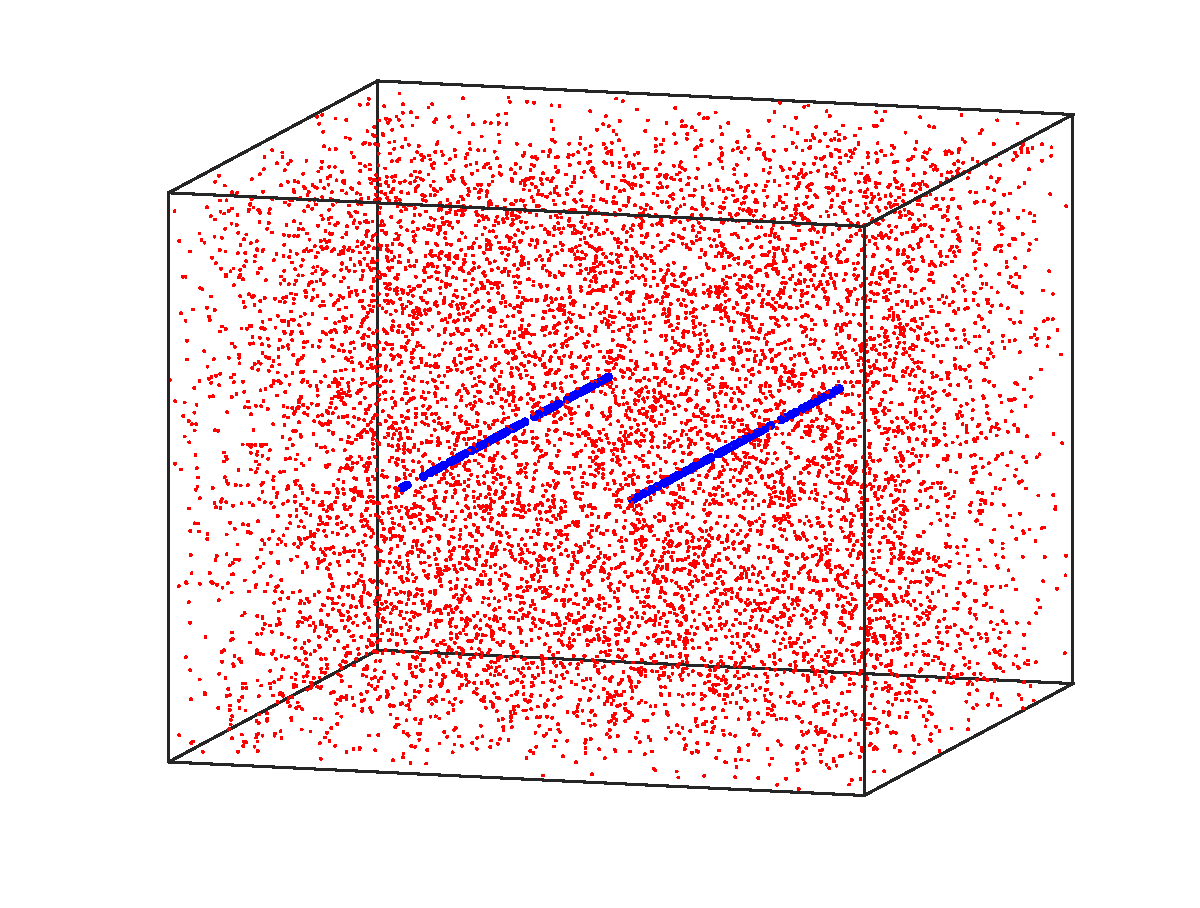
\includegraphics[width=0.8\columnwidth]{gasandwires3.eps}
\\ Two wires of fermions in 3D BEC. In blue: fermions. In red: bosons.  
\end{figure}

\newpage

% Chapter 3

\chapter{Induced interaction} % Main chapter title

\label{Chapter3} % For referencing the chapter elsewhere, use \ref{Chapter3} 

\lhead{Part II. \emph{Kitaev wires}}
\chead{Chapter 3. \emph{Induced interaction}} % This is for the header on each page - perhaps a shortened title

%----------------------------------------------------------------------------------------
In this chapter we derive the induced interactions between the fermions on the wires. First stop is to look at the effective interaction between the fermions on the wires and the bosons in the condensate.
\section{Effective Bose-Fermi interaction}
The effective interaction between the fermions ($F$) and the bosons ($B$) is modelled by a delta function potential with strength $g_{BF}$: $V(\mathbf{r})=g_{BF}\delta(\mathbf{r})$. This means, that the \textit{int}eraction Hamiltonian for the effective pair interaction reads:
\begin{equation}
H_{BF}^\text{int}  = \int d^3 r d^3 r' \; \psi_F^\dagger(\mathbf{r}) \psi_B^\dagger(\mathbf{r}')V(\mathbf{r}-\mathbf{r}')\psi_B(\mathbf{r}')\psi_F(\mathbf{r}) = g_{BF}\int d^3 r \; \psi_F^\dagger(\mathbf{r}) \psi_B^\dagger(\mathbf{r})\psi_B(\mathbf{r})\psi_F(\mathbf{r}),
\label{eq.HintBF}
\end{equation}
where $\psi_i(\mathbf{r})$ is the field operator for the $i$-particles, and so $\psi_i^\dagger(\mathbf{r})$ creates a particle at position $\mathbf{r}$.\footnote{The subscript $BF$ specifies, that it is the Hamiltonian for the interaction between bosons and fermions.} Notice, that there is no factor of $1/2$ in front of the integrals. As noted in section \ref{sec.secondquantization} the factor of $1/2$ should be omitted, when the particles are distinguishable, as fermions and bosons most certainly are. 

The fermions ($F$) are confined to two one-dimensional wires. Let the first one be along the $x$-axis, the second at $z = d, y = 0$. The confinement is provided by two harmonic traps in the $y$- and $z$-directions with the same trapping frequency $\omega_t$.\footnote{This is mostly for simplicity. It can easily be generalized to different trapping frequencies $\omega_y$ and $\omega_z$ for the two directions.} In this connection we have two central assumptions. Firstly, we require that the fermions are trapped in the ground state with respect to the perpendicular directions. The energy gap from the ground state to the first excited state is $\omega_t$. Hence by making $\omega_t$ sufficiently large we trap the fermions in the lowest lying state, $\phi_0$, along the two wires. Specifically, the typical energy of the fermions is the free gas Fermi energy $\epsilon_{F,0} = \frac{k_F^2}{2m_F}$. Hence, we require $\frac{\epsilon_{F,0}}{\omega_t} \ll 1$. Using the trapping width $l_t = \frac{1}{\sqrt{m_F\omega_t}}$, we can also express this as $(k_Fl_t)^2 \ll 1$. One might be afraid of violating the Pauli exclusion principle in this context. However, the states in the $x$-direction are allowed to be different, and so we can symmetrize in the $y$- and $z$-directions.

The second assumption is, that the distance between the wires is much larger than the trapping width of the wires, $l_t$. Hence, $l_t/d \ll 1$. This is done, so that we can actually talk about distinguishable wires of fermions. This leads to the following expansion in momentum eigenstates:
\begin{equation}
\psi_F(x,\mathbf{r}_\perp) = \frac{1}{\sqrt{\mathcal{L}}}\sum_p \text{e}^{ipx} \left[\phi_0(\mathbf{r}_\perp) c_{1,p} + \phi_0(\mathbf{r}_\perp - \mathbf{d}) c_{2,p}\right], \hspace{0.5cm} \psi_B(\mathbf{r}) = \frac{1}{\sqrt{\mathcal{V}}}\sum_{\mathbf{k}} \text{e}^{i\mathbf{k}\cdot \mathbf{r}} b_\mathbf{k}, 
\end{equation}  
with $\phi_0(\mathbf{r}_\perp) = \frac{1}{\sqrt{\pi}l_t}\exp\left(-\frac{r_\perp^2}{2l_t^2}\right)$ the harmonic ground state with respect to the perpendicular directions and $\mathbf{d} = d\cdot\hat{z}$ the position of wire 2. $c^\dagger_{j,p}$ creates a fermion in wire $j$ with momentum $p$. $b^\dagger_\mathbf{k}$ creates a boson with momentum $\mathbf{k}$.  We assume, that the wires are truly distinguishable. This means that all anticommutators like $\{c_{1,p}, c^\dagger_{2,p'}\}$ vanish. Inserting these expressions into $H_{BF}^\text{int}$ yields in total four terms. However, the cross terms where a fermion is annihilated in one wire and created in the other are proportional to the integral: $\int d^2 r_\perp \phi_0(\mathbf{r}_\perp)\phi_0(\mathbf{r}_\perp-\mathbf{d}) = 0$. The integral is negligible, because by assumption $l_t/d \ll 1$. The terms arising from interactions with fermions in wire 1 are:
\begin{equation}
H_{BF, 1}^{\text{int}} = \frac{g_{BF}}{\mathcal{LV}}\int d^3 r \sum_{p,p',q,q'}\sum_{\mathbf{k}_{\perp},\mathbf{k}_{\perp}'}\text{e}^{i((p-p')+(q-q'))x} \phi^2_0(\mathbf{r}_{\perp})\text{e}^{i(\mathbf{k}_{\perp} - \mathbf{k}_{\perp}')\cdot \mathbf{r}_\perp} c^\dagger_{1,p'} b^\dagger_{q',\mathbf{k}_\perp'}b_{q,\mathbf{k}_\perp}c_{1,p}. \nonumber
\end{equation}
The integral over $x$ yields the factor $\mathcal{L}\delta_{p-p',q'-q}$, implying total momentum conservation along the wire. The integral over $\mathbf{r}_\perp$ gives the Fourier transform of $\phi_0^2(\mathbf{r}_\perp)$. Since $\phi_0$ is a gaussian, the Fourier transform is as well. Explicitly: $\int d^2 r_\perp \; \phi^2_0(\mathbf{r}_{\perp})\text{e}^{i(\mathbf{k}_{\perp}-\mathbf{k}_{\perp}')\cdot \mathbf{r}_\perp} = \text{e}^{-\frac{l_t^2}{4}(\mathbf{k}_{\perp}-\mathbf{k}_{\perp}')^2}$. Taking the sum over $q'$ forces $q' = p - p' + q$. In total:
\begin{align}
H_{BF, 1}^{\text{int}} &= \frac{g_{BF}}{\mathcal{V}}\sum_{p, p', q} \sum_{\mathbf{k}_\perp, \mathbf{k}_\perp'} \text{e}^{-\frac{l_t^2}{4}(\mathbf{k}_\perp-\mathbf{k}_\perp')^2} c^\dagger_{1, p'} b^\dagger_{p - p' + q, \mathbf{k}_\perp'} b_{q, \mathbf{k}_\perp}c_{1, p} \nonumber \\
                  &= \frac{g_{BF}}{\mathcal{V}}\sum_{p_1, p_2, q} \sum_{\mathbf{k}_\perp, \mathbf{k}_\perp'} \text{e}^{-\frac{l_t^2}{4}(\mathbf{k}_\perp-\mathbf{k}_\perp')^2} c_{1, p_2 - q}^\dagger b_{p_1 + q, \mathbf{k}_\perp'}^\dagger b_{p_1, \mathbf{k}_\perp}c_{1, p_2}.
\end{align}
The last line is obtained by appropriate renaming. To be very specific: $p_1, p_2$ and $q$ are in the $x$ direction, along wire 1, whilst $\mathbf{k}_\perp'$ and $\mathbf{k}_\perp$ are momenta in the $(y,z)$-plane, hence perpendicular to wire 1. The interactions with fermions in wire 2 yields a very similar result. The only alteration is, that $\phi_0(\mathbf{r}_\perp) \to \phi_0(\mathbf{r}_\perp - \mathbf{d})$. The above Fourier transformation therefore yields an additional phase of $\text{e}^{i(\mathbf{k}_\perp - \mathbf{k}_\perp')\cdot \mathbf{d}}$. In total the interaction Hamiltonian hereby becomes:
\begin{align}
H_{BF}^\text{int} = \frac{g_{BF}}{\mathcal{V}}\sum_{p_1,p_2,q} \sum_{\mathbf{k}_\perp, \mathbf{k}_\perp'} & \text{e}^{-\frac{l_t^2}{4}(\mathbf{k}_\perp - \mathbf{k}_\perp')^2}\left[ c^\dagger_{1,p_2-q} b^\dagger_{p_1+q, \mathbf{k}_\perp'} b_{p_1,\mathbf{k}_\perp}c_{1,p_2} + \right. \nonumber \\
& \left. \text{e}^{i(\mathbf{k}_\perp - \mathbf{k}_\perp')\cdot \mathbf{d}}c_{2,p_2-q}^\dagger b_{p_1+q, \mathbf{k}_\perp'}^\dagger b_{p_1,\mathbf{k}_\perp}c_{2,p_2} \right].
\end{align}
This shows, that a scattering event in wire 1 is associated with the factor $g_{BF} \text{e}^{-\frac{l_t^2}{4}(\mathbf{k}_\perp - \mathbf{k}_\perp')^2}$, and that the corresponding scattering in wire 2 has an extra factor of $\text{e}^{i(\mathbf{k}_\perp - \mathbf{k}_\perp')\cdot \mathbf{d}}$. In both cases the transverse momenta are free. An obvious thing to do now would be to take the limit $\omega_t \to \infty$ or equivalently $l_t \to 0$. However, as we shall see later, it will be crucial to keep the trapping frequency finite, at least at the present stage.  

\section{1D-3D induced interactions} \label{sec.1D3Dinducedinteraction}
\subsection{Feynman diagrams} \label{subsec.Feynmandiagrams}
The bosons are assumed to be in a perfect Bose-Einstein condensate (BEC). This means, that they are essentially lying still. We are further only interested in the weak coupling limit.\footnote{There is a small fraction in nonzero momenta states, which is neglected. It would be necessary to include this for stronger interactions.} In a more general setup, one would have to calculate contributions from increasing orders in the underlying bare interaction leading to a socalled $T$-matrix, but this will not be pursued here. We will write the coupling strength as $g_{BF} = \frac{2\pi a_{BF}}{m_r}$, with $m_r = \frac{m_Fm_B}{m_B + m_F}$ the reduced mass, and $a_{BF}$ the effective scattering length. In a formally precise manner one can expand the $T$-matrix in orders of $a_{BF}$. From this analysis, it is clear that the smallness of the coupling strength is equivalent to demanding $(n_Ba_{BF}^3)^{1/3}\ll 1$. We can also argue for this by a dimensional analysis. From the form of $g_{BF}$ it is clear, that we should argue from $a_{BF}$. This has dimension of length, and so we need a parameter of dimension per length to get a unitless expression. The only reasonable parameter is the one that describes how many bosons, the fermions can actually interact with, leading to a length scale $n_B^{-1/3}$. Since a higher density of bosons leads to more fermion-boson interactions, we should therefore assume $(n_Ba_{BF}^3)^{1/3} \ll 1$. In this weak coupling limit we can safely take interactions only up to second order in $g_{BF}$. This means, that the four essential diagrams for the fermion-fermion induced interaction are the ones showed in figure \ref{fig.feynmandiagrams}. 

\begin{figure}
\begin{tikzpicture}[scale=0.25]
  \begin{feynman}[small]
    \vertex (number1) {\( (1) \)};
    \vertex [above left=of number1] (fermion1) {\( \tilde{p}_1 \)};
    \vertex [above right=of fermion1] (a);
    \vertex [below right=of a] (fermion2) {\(\tilde{p}_1 + \tilde{q}\)}; 
    \vertex [above=of a] (b);
    \vertex [left=of b] (boson1) {\( \sqrt{n_B} \)}; 
    \vertex [above= of b] (c);
    \vertex [right= of c] (boson2) {\( \sqrt{n_B} \)};
    \vertex [above= of c] (d);
    \vertex [above left=of d] (f3) {\(\tilde{p}_2\)};
    \vertex [above right=of d] (f4) {\(\tilde{p}_2 - \tilde{q}\)};
 
    \diagram* {
      (number1) -- [opacity=0.0] (fermion1) -- [fermion] (a) -- [fermion] (fermion2),
      (a) -- [photon, edge label'=\(g_{BF}\)] (b),
      (b) -- [dashed] (boson1),
      (b) -- [blue, fermion, edge label' = {\(-\tilde{q}, \mathbf{k}_\perp \)}] (c),
      (c) -- [dashed] (boson2),
      (c) -- [photon, edge label'=\(g_{BF}\)] (d),
      (d) -- [anti fermion] (f3),
      (d) -- [fermion] (f4)
    };
  \end{feynman}
\end{tikzpicture}
\begin{tikzpicture}
  \begin{feynman}[small]
    \vertex (number2) {\( (2) \)};
    \vertex [above left=of number2] (fermion1) {\( \tilde{p}_1 \)};
    \vertex [above right=of fermion1] (a);
    \vertex [below right=of a] (fermion2) {\(\tilde{p}_1 + \tilde{q}\)}; 
    \vertex [above=of a] (b);
    \vertex [left=of b] (boson1) {\( \sqrt{n_B} \)}; 
    \vertex [above= of b] (c);
    \vertex [right= of c] (boson2) {\( \sqrt{n_B} \)};
    \vertex [above= of c] (d);
    \vertex [above left=of d] (f3) {\(\tilde{p}_2\)};
    \vertex [above right=of d] (f4) {\(\tilde{p}_2 - \tilde{q}\)};
 
    \diagram* {
      (number2) -- [opacity=0.0] (fermion1) -- [fermion] (a) -- [fermion] (fermion2),
      (a) -- [photon, edge label'=\(g_{BF}\)] (b),
      (b) -- [dashed] (boson1),
      (b) -- [blue, anti fermion, edge label' = {\(\tilde{q}, \mathbf{k}_\perp \)}] (c),
      (c) -- [dashed] (boson2),
      (c) -- [photon, edge label'=\(g_{BF}\)] (d),
      (d) -- [anti fermion] (f3),
      (d) -- [fermion] (f4)
    };
  \end{feynman}
\end{tikzpicture}
\begin{tikzpicture}
  \begin{feynman}[small]
    \vertex (number3) {\( (3) \)};
    \vertex [above left=of number3] (fermion1) {\( \tilde{p}_1 \)};
    \vertex [above right=of fermion1] (a);
    \vertex [below right=of a] (fermion2) {\(\tilde{p}_1+\tilde{q}\)}; 
    \vertex [above=of a] (b);
    \vertex [left=of b] (boson1) {\( \sqrt{n_B} \)}; 
    \vertex [above= of b] (c);
    \vertex [right= of c] (boson2) {\( \sqrt{n_B} \)};
    \vertex [above= of c] (d);
    \vertex [above left=of d] (f3) {\(\tilde{p}_2\)};
    \vertex [above right=of d] (f4) {\(\tilde{p}_2-\tilde{q}\)};
 
    \diagram* {
      (number3) -- [opacity=0.0] (fermion1) -- [fermion] (a) -- [fermion] (fermion2),
      (a) -- [photon, edge label'=\(g_{BF}\)] (b),
      (b) -- [dashed] (boson1),
      (b) -- [blue, majorana, edge label' = {\(\tilde{q}, \mathbf{k}_\perp \)}] (c),
      (c) -- [dashed] (boson2),
      (c) -- [photon, edge label'=\(g_{BF}\)] (d),
      (d) -- [anti fermion] (f3),
      (d) -- [fermion] (f4)
    };
  \end{feynman}
\end{tikzpicture}
\begin{tikzpicture}
  \begin{feynman}[small]
    \vertex (number4) {\( (4) \)};
    \vertex [above left=of number4] (fermion1) {\( \tilde{p}_1 \)};
    \vertex [above right=of fermion1] (a);
    \vertex [below right=of a] (fermion2) {\(\tilde{p}_1+\tilde{q}\)}; 
    \vertex [above=of a] (b);
    \vertex [left=of b] (boson1) {\( \sqrt{n_B} \)}; 
    \vertex [above= of b] (c);
    \vertex [right= of c] (boson2) {\( \sqrt{n_B} \)};
    \vertex [above= of c] (d);
    \vertex [above left=of d] (f3) {\(\tilde{p}_2\)};
    \vertex [above right=of d] (f4) {\(\tilde{p}_2-\tilde{q}\)};
 
    \diagram* {
      (number3) -- [opacity=0.0] (fermion1) -- [fermion] (a) -- [fermion] (fermion2),
      (a) -- [photon, edge label'=\(g_{BF}\)] (b),
      (b) -- [dashed] (boson1),
      (b) -- [blue, anti majorana, edge label' = {\(\tilde{q}, \mathbf{k}_\perp \)}] (c),
      (c) -- [dashed] (boson2),
      (c) -- [photon, edge label'=\(g_{BF}\)] (d),
      (d) -- [anti fermion] (f3),
      (d) -- [fermion] (f4)
    };
  \end{feynman}
\end{tikzpicture}
\caption{Feynman diagrams for the induced interaction. Since the interaction is weak, we can neglect all other Feynman diagrams than (1)-(4). Diagrams (1) and (2) stems from the normal Green's function $G_{11}$. Diagrams (3) and (4) stems from the anormalous Green's functions $G_{12}$ and $G_{21}$. The diagrams have the exact same form for interactions between fermions in the same and opposite wires. The only difference is, that $g_{BF}$ carries an extra phase factor for interactions in wire 2. } 
\label{fig.feynmandiagrams}
\end{figure}

Notice that the bosons of the BEC, shown with dashed lines, carry a factor of $\sqrt{n_B}$. This is simply because it is the pour condensate wave function. Further $\tilde{p}_j = (p_j, i\omega_{m_j})$, with $\omega_{m} = (2m + 1)\pi kT$ a fermionic Matsubara frequency, and $\tilde{q} = (q, i\omega_q )$, with $\omega_q = \omega_{m_1} - \omega_{m_2}$ a bosonic Matsubara frequency. The blue lines in the diagrams are the normal and anormalous Bogoliubov phonon Green's functions derived in subsection \ref{sec.BECGreens}. Functionally they are:
\begin{equation}
G_{11}(\mathbf{k},i\omega_m) = \frac{u_{B,k}^2}{i\omega_m-E_{B,k}}-\frac{v_{B,k}^2}{i\omega_m+E_{B,k}}, \hspace{0.5cm} G_{12}(\mathbf{k},i\omega_m) = G_{21}(\mathbf{k},i\omega_m) = \frac{u_{B,k}v_{B,k}}{i\omega_m+E_{B,k}}-\frac{u_{B,k}v_{B,k}}{i\omega_m-E_{B,k}}.\nonumber
\end{equation}
Here $u_{B,k}$ and $v_{B,k}$ are the BEC coherence factors found in subsection \ref{sec.BEC} with $m_B$ the mass of the bosons. Further $E^2_{B,k} = \frac{k^2}{2m_B}\left(\frac{k^2}{2m_B} + 2g_Bn_B \right)$ is the BEC Bogoliubov spectrum and $g_B = \frac{4\pi a_B}{m_B}$, with $a_B$ the scattering length in the BEC. The diagrams can intuitively be understood as follows. A fermion in one wire interact with a (real) boson in the condensate. This creates a ripple in the condensate described by one of the Green's functions. This ripple reaches a second fermion in one of the two wires, where the momentum of the ripple is transferred to.  

Let us first focus on the induced interaction of two fermions in wire 1. Since the perpendicular momentum $\mathbf{k}_\perp$ is completely free we have to integrate over this. Since the momentum of the incoming and outgoing boson in each diagram is 0 we simply get a factor of $g_{BF}\; \text{e}^{-\frac{l_t^2}{4}k_\perp^2}$ \textit{twice}. Collecting all factors gives us the four contributions from the four diagrams (1)-(4) to the fermion-fermion induced interaction $V_{\text{ind}}^{11}$: 
\begin{align}
V^{11}_{\text{ind}, 1}(q,i\omega_q) &= n_Bg_{BF}^2\int\frac{d^2k_\perp}{(2\pi)^2}G_{11}(-q,\mathbf{k}_\perp,-\omega_q)\text{e}^{-\frac{l_t^2}{2}k_\perp^2}, \nonumber \\
V^{11}_{\text{ind}, 2}(q,i\omega_q) &= n_Bg_{BF}^2\int\frac{d^2k_\perp}{(2\pi)^2}G_{11}(q,\mathbf{k}_\perp,\omega_q)\text{e}^{-\frac{l_t^2}{2}k_\perp^2}, \nonumber \\
V^{11}_{\text{ind}, 3}(q,i\omega_q) &= n_Bg_{BF}^2\int\frac{d^2k_\perp}{(2\pi)^2}G_{12}(q,\mathbf{k}_\perp,\omega_q)\text{e}^{-\frac{l_t^2}{2}k_\perp^2}, \nonumber \\
V^{11}_{\text{ind}, 4}(q,i\omega_q) &= n_Bg_{BF}^2\int\frac{d^2k_\perp}{(2\pi)^2}G_{12}(q,\mathbf{k}_\perp,\omega_q)\text{e}^{-\frac{l_t^2}{2}k_\perp^2}. 
\end{align}
We notice, that the last two give the same contribution in this weak interacting limit.\footnote{This would \textit{not} be the case, when including higher order terms.} The 11 superscript means, that it is for two fermions in wire 1. Summing up the four contributions gives us the frequency dependent induced interaction $V^{11}_{\text{ind}}$ for fermions in wire 1:
\begin{equation}
V^{11}_{\text{ind}}(q,i\omega_q) = g_{BF}^2\int\frac{d^2k_\perp}{(2\pi)^2}\; \chi_\text{BEC}(q,\mathbf{k}_\perp,i\omega_q)\text{e}^{-\frac{l_t^2}{2}k_\perp^2}, 
\label{eq.V11indXBEC}
\end{equation}
with $\chi_\text{BEC}(\mathbf{k},i\omega_q) = \frac{k^2}{m_B}\frac{n_B}{(i\omega_q)^2 - E_{B,k}^2}$ the socalled density-density correlation function of the BEC. It now becomes clear, why we had to retain a nonzero value of $l_t$ at this stage. For $l_t\to 0$ the above has an integrand of the form $k^2/(ak^4 + bk^2 + c)$, with $a,b,c$ positive constants. As a result the integral is logarithmically divergent. The situation in a 2D-3D system is different. Here there is a single integral in the above, and the result converges for $l_t\to 0$. We return to this later on. For two fermions in wire 2, there is two additional phase factors. The incoming boson is associated with $\text{e}^{i\mathbf{k}_\perp\cdot \mathbf{d}}$, the outgoing with $\text{e}^{-i\mathbf{k}_\perp\cdot \mathbf{d}}$. These phase factors cancel and $V^{22}_{\text{ind}}(q,i\omega_q) = V^{11}_{\text{ind}}(q,i\omega_q)$ as one would expect. We denote these \textit{intra}wire interactions. Additionally, there is an \textit{inter}wire induced interaction between the wires, which we will denote $V_{\text{ind}}^{12}(q,i\omega_q)$. The preceding section shows, that the calculation of this induced interaction is analogous to the above, but with the additional factor of $\text{e}^{i\mathbf{k}_\perp\cdot \mathbf{d}}$ from scattering in the second wire. Hence:
\begin{equation}
V_{\text{ind}}^{12}(q,i\omega_q) = g_{BF}^2\int\frac{d^2k_\perp}{(2\pi)^2}\; \chi_\text{BEC}(q,\mathbf{k}_\perp, i\omega_q)\text{e}^{-\frac{l_t^2}{2}k_\perp^2}\text{e}^{i\mathbf{k}_\perp\cdot \mathbf{d}}. 
\label{eq.V12indXBEC} 
\end{equation}
We notice, that the \textit{inter}wire interaction goes to the \textit{intra}wire interaction for $d \to 0$. The presence of the condensate density-density correlation expresses, that it is density fluctuations in the condensate that mediate the induced interactions. It turns out, that we can find quite simple expressions for these induced interactions in real space in the zero frequency limit: $\omega_q = 0$. Since we in general are going to restrict ourselves to this limit, we briefly discuss what it physically means. 

\subsection{Retardation effects} \label{sec.RetardationEffects}
From equations \eqref{eq.V11indXBEC} and \eqref{eq.V12indXBEC} it is evident that the induced interactions have a frequency dependency. This dependency reflects, that the fermions do not interact instanteneously, socalled retardation effects. In turn this embodies, that the phonons in the condensate, the mediators of the fermion-fermion interaction, moves at a finite speed $c_0 = \sqrt{\frac{n_Bg_B}{m_B}} = \frac{\sqrt{4\pi n_B a_B}}{m_B}$.\footnote{It is analogous to the retarded fields in electrodynamics. There it reflects the finiteness of the speed of light.} To neglect these effects we therefore need to assume, that the typical speed of the fermions is much smaller than the speed of the bosons: $v_F \ll c_0$, $v_F = k_F/m_F$ the Fermi speed for free fermions. This leads to the relation:
\begin{equation}
1 \gg \frac{v_F}{c_0} = \frac{\sqrt{\pi}}{2} \frac{m_B}{m_F}\frac{1}{ \sqrt{ (n_Ba_B^3)^{1/3} } }\frac{n_F}{ n_B^{1/3} } = \frac{m_B}{m_F}\frac{k_F\xi}{\sqrt{2}}, 
\label{eq.RetardationEffectsneglectionassumption}
\end{equation}
whereby we have expressed the ratio of velocities in terms of unitless quantities and in terms of the coherence length, $\xi$, defined by $\frac{1}{\xi^2} = 2m_Bn_Bg_B$. With this assumption at hand we can focus on the zero frequency induced interaction $V^{ij}_{\text{ind}}(q,0)$. For fermions and bosons of similar mass we notice, that the neglect of retardation effects is equivalent to only studying short range interactions: $k_F\xi \lesssim 1$. 

\subsection{Real space}
\label{subsec.inducedinteraction.realspace}
In this subsection we calculate the real space interactions, $\tilde{V}^{ij}_{\text{ind}}(x, 0)$. 

We start with the \textit{inter}wire interaction. We get:
\begin{equation}
\tilde{V}^{12}_{\text{ind}}(x, 0) = \int \frac{dq}{2\pi} \; \text{e}^{iqx} V^{12}_{\text{ind}}(q, 0) = g^2_{BF}\int \frac{d^3 k}{(2\pi)^3}\;\chi_\text{BEC}(\mathbf{k}, 0)\text{e}^{-\frac{l_t^2}{2}k_\perp^2}\text{e}^{i\mathbf{k}\cdot \mathbf{r}}, \nonumber
\end{equation}
where we write $\mathbf{k} = (q, \mathbf{k}_{\perp})$ and $\mathbf{r} = (x, \mathbf{r}_{\perp})$. The above expression converges for $l_t \to 0$, because the integrand is monotonically increasing for decreasing $l_t$. The gaussian, $\text{e}^{-\frac{l_t^2}{2}k_\perp^2}$, hereby drops out and we are left with the Fourier transformation of $\chi_\text{BEC}(\mathbf{k}, 0) = -4m_Bn_B\frac{1}{k^2 + 1/\xi^2}$. We recognise this as the Yukawa potential in momentum space. For completeness we here show how to perform the Fourier transformation. The integral of interest is:
\begin{equation}
I(\mathbf{r}) = \int \frac{d^3 k}{(2\pi)^3} \frac{1}{k^2 + 1/\xi^2}\text{e}^{i\mathbf{k}\cdot\mathbf{r}} = \int_{0}^{\pi}d\theta \sin(\theta)\int_{0}^{\infty}\frac{dk}{(2\pi)^2} \frac{k^2}{k^2 + 1/\xi^2}\text{e}^{ikr\cos(\theta)},
\label{eq.def.Fourierintegral}
\end{equation}
where we in the second expression set the angle between $\mathbf{k}$ and $\mathbf{r}$ to be $\theta$ and transform the integral to polar coordinates. We have further used, that the integrand does not depend on the azimuthal angle, $\phi$, so that this integral simple yields a factor of $2\pi$. The $\theta$ dependent part then simply gives:
\begin{equation}
\int_{0}^{\pi}d\theta \sin(\theta)\text{e}^{ikr\cos(\theta)} = -\left.\frac{1}{ikr}\text{e}^{ikr\cos(\theta)}\right|_{0}^{\pi} = \frac{1}{ikr}\left(\text{e}^{ikr} - \text{e}^{-ikr}\right). \nonumber
\end{equation}
Inserting this into equation \eqref{eq.def.Fourierintegral} yields: $I(\mathbf{r}) = \frac{1}{2\pi r}\int \frac{dk}{2\pi i} \frac{k}{k^2 + 1/\xi^2}\text{e}^{ikr}$, where the integration limits are now implicitly $\pm \infty$. This integral is solvable using Cauchy's residue theorem. Explicitly, we now think of $k$ as a complex variable. We define the half-circle contour $\mathcal{C}$ in the upper half-plane with a radius $R$ tending to infinity. Since $r > 0$ the integrand goes exponentially to zero at the circle boundary, so that this part of the contour integral does not contribute. We have to find the poles of the integrand in the upper complex plane of $k$ and calculate the residues. There is a single pole given by $k = \frac{i\sqrt{2}}{\xi}$. Cauchy's residue theorem then states, that:
\begin{equation}
I(\mathbf{r}) = \frac{1}{2\pi r}\int \frac{dk}{2\pi i} \frac{k}{k^2 + 1/\xi^2}\text{e}^{ikr} = \frac{1}{2\pi r}\text{Res}\left(\frac{k}{k^2 + 1/\xi^2}\text{e}^{ikr}, \frac{i\sqrt{2}}{\xi}\right) = \frac{1}{4\pi r} \text{e}^{-\sqrt{2}r/\xi}, \nonumber
\end{equation}
where $\text{Res}(f(x), x_0)$ denotes the residue of $f(x)$ in $x = x_0$. Setting $\mathbf{r} = (x, \mathbf{d})$ we get for the induced interaction between the wires:
\begin{equation}
\tilde{V}^{12}_{\text{ind}}(x, 0) = -4m_Bg^2_{BF}n_B I(x, \mathbf{d}) = -\frac{m_Bg_{BF}^2n_B}{\pi}\frac{\text{e}^{ -\sqrt{2}\sqrt{x^2 + d^2}/\xi }}{\sqrt{x^2 + d^2}}.
\label{eq.V12indx}
\end{equation}
As noted in section \ref{sec.1D3Dinducedinteraction} we can obtain the intrawire interaction by simply setting $d = 0$. We get:
\begin{equation}
\tilde{V}^{11}_{\text{ind}}(x, 0) = -\frac{m_Bg_{BF}^2n_B}{\pi}\frac{\text{e}^{ -\sqrt{2}|x|/\xi }}{|x|}.
\label{eq.V11indx}
\end{equation}
The induced interaction in real space is seen to be the Yukawa interaction with a range of interaction given by the BEC coherence length, $\xi$. We can also understand this physically. The coherence length is in general the length scale over which, the condensate adjusts to an influence on the boson density. Hence, it is physically intuitive that this is exactly the range of the interaction. 

We could have calculated the intrawire induced interaction for a general $l_t > 0$ and then taken the $l_t \to 0$ limit. The reader is referred to appendix \ref{Appendix.intrawireinteraction.ltnonzero} to see this explicitly. In the end it gives the same result. 

We get a unitless form of the real space interaction by dividing with the typical energy of the fermions, the Fermi energy $\epsilon_{F,0}$. In this way the resulting front factor of $\tilde{V}^{ij}_{\text{ind}} / \epsilon_{F,0}$ is a measure of the strength of interaction given by:
\begin{equation}
G = - 8\left( \frac{m_F}{m_B} + \frac{m_B}{m_F} + 2 \right) \frac{n_B^{1/3}}{n_F}(n_Ba_{BF}^3)^{2/3}.
\label{eq.interactionstrength.wires}
\end{equation}
The mass ratio $m_B / m_F$, The relative interparticle distance $n_B^{1/3} / n_F$ and the Bose-Fermi gas parameter $(n_Ba_{BF}^3)^{1/3}$ hereby comes naturally about by going to unitless quantities. 

In figure \ref{fig.V12indx} we show the interwire interaction for several interwire distances, $d$. The black curve is the $d = 0$ limit where the inter- and intrawire interactions coincide. 

\begin{figure} 
\begin{center}  
% GNUPLOT: LaTeX picture with Postscript
\begingroup
  \makeatletter
  \providecommand\color[2][]{%
    \GenericError{(gnuplot) \space\space\space\@spaces}{%
      Package color not loaded in conjunction with
      terminal option `colourtext'%
    }{See the gnuplot documentation for explanation.%
    }{Either use 'blacktext' in gnuplot or load the package
      color.sty in LaTeX.}%
    \renewcommand\color[2][]{}%
  }%
  \providecommand\includegraphics[2][]{%
    \GenericError{(gnuplot) \space\space\space\@spaces}{%
      Package graphicx or graphics not loaded%
    }{See the gnuplot documentation for explanation.%
    }{The gnuplot epslatex terminal needs graphicx.sty or graphics.sty.}%
    \renewcommand\includegraphics[2][]{}%
  }%
  \providecommand\rotatebox[2]{#2}%
  \@ifundefined{ifGPcolor}{%
    \newif\ifGPcolor
    \GPcolortrue
  }{}%
  \@ifundefined{ifGPblacktext}{%
    \newif\ifGPblacktext
    \GPblacktexttrue
  }{}%
  % define a \g@addto@macro without @ in the name:
  \let\gplgaddtomacro\g@addto@macro
  % define empty templates for all commands taking text:
  \gdef\gplbacktext{}%
  \gdef\gplfronttext{}%
  \makeatother
  \ifGPblacktext
    % no textcolor at all
    \def\colorrgb#1{}%
    \def\colorgray#1{}%
  \else
    % gray or color?
    \ifGPcolor
      \def\colorrgb#1{\color[rgb]{#1}}%
      \def\colorgray#1{\color[gray]{#1}}%
      \expandafter\def\csname LTw\endcsname{\color{white}}%
      \expandafter\def\csname LTb\endcsname{\color{black}}%
      \expandafter\def\csname LTa\endcsname{\color{black}}%
      \expandafter\def\csname LT0\endcsname{\color[rgb]{1,0,0}}%
      \expandafter\def\csname LT1\endcsname{\color[rgb]{0,1,0}}%
      \expandafter\def\csname LT2\endcsname{\color[rgb]{0,0,1}}%
      \expandafter\def\csname LT3\endcsname{\color[rgb]{1,0,1}}%
      \expandafter\def\csname LT4\endcsname{\color[rgb]{0,1,1}}%
      \expandafter\def\csname LT5\endcsname{\color[rgb]{1,1,0}}%
      \expandafter\def\csname LT6\endcsname{\color[rgb]{0,0,0}}%
      \expandafter\def\csname LT7\endcsname{\color[rgb]{1,0.3,0}}%
      \expandafter\def\csname LT8\endcsname{\color[rgb]{0.5,0.5,0.5}}%
    \else
      % gray
      \def\colorrgb#1{\color{black}}%
      \def\colorgray#1{\color[gray]{#1}}%
      \expandafter\def\csname LTw\endcsname{\color{white}}%
      \expandafter\def\csname LTb\endcsname{\color{black}}%
      \expandafter\def\csname LTa\endcsname{\color{black}}%
      \expandafter\def\csname LT0\endcsname{\color{black}}%
      \expandafter\def\csname LT1\endcsname{\color{black}}%
      \expandafter\def\csname LT2\endcsname{\color{black}}%
      \expandafter\def\csname LT3\endcsname{\color{black}}%
      \expandafter\def\csname LT4\endcsname{\color{black}}%
      \expandafter\def\csname LT5\endcsname{\color{black}}%
      \expandafter\def\csname LT6\endcsname{\color{black}}%
      \expandafter\def\csname LT7\endcsname{\color{black}}%
      \expandafter\def\csname LT8\endcsname{\color{black}}%
    \fi
  \fi
    \setlength{\unitlength}{0.0500bp}%
    \ifx\gptboxheight\undefined%
      \newlength{\gptboxheight}%
      \newlength{\gptboxwidth}%
      \newsavebox{\gptboxtext}%
    \fi%
    \setlength{\fboxrule}{0.5pt}%
    \setlength{\fboxsep}{1pt}%
\begin{picture}(7200.00,5040.00)%
    \gplgaddtomacro\gplbacktext{%
      \csname LTb\endcsname%
      \put(682,1188){\makebox(0,0)[r]{\strut{}$-4$}}%
      \csname LTb\endcsname%
      \put(682,2030){\makebox(0,0)[r]{\strut{}$-2$}}%
      \csname LTb\endcsname%
      \put(682,2872){\makebox(0,0)[r]{\strut{}$0$}}%
      \csname LTb\endcsname%
      \put(682,3713){\makebox(0,0)[r]{\strut{}$2$}}%
      \csname LTb\endcsname%
      \put(682,4555){\makebox(0,0)[r]{\strut{}$4$}}%
      \csname LTb\endcsname%
      \put(877,484){\makebox(0,0){\strut{}$-10$}}%
      \csname LTb\endcsname%
      \put(2343,484){\makebox(0,0){\strut{}$-5$}}%
      \csname LTb\endcsname%
      \put(3809,484){\makebox(0,0){\strut{}$0$}}%
      \csname LTb\endcsname%
      \put(5274,484){\makebox(0,0){\strut{}$5$}}%
      \csname LTb\endcsname%
      \put(6740,484){\makebox(0,0){\strut{}$10$}}%
    }%
    \gplgaddtomacro\gplfronttext{%
      \csname LTb\endcsname%
      \put(176,2871){\rotatebox{-270}{\makebox(0,0){\strut{}$2m_F/k_F W_{	ext{ind}}(k, k_F)$}}}%
      \put(3808,154){\makebox(0,0){\strut{}$k / k_F$}}%
      \csname LTb\endcsname%
      \put(4565,4803){\makebox(0,0)[l]{\strut{}$k_Fd = 0.720$}}%
      \csname LTb\endcsname%
      \put(4565,4583){\makebox(0,0)[l]{\strut{}$k_Fd = 0.735$}}%
      \csname LTb\endcsname%
      \put(4565,4363){\makebox(0,0)[l]{\strut{}$k_Fd = 0.750$}}%
      \csname LTb\endcsname%
      \put(4565,4143){\makebox(0,0)[l]{\strut{}$k_Fd = 0.765$}}%
      \csname LTb\endcsname%
      \put(4565,3923){\makebox(0,0)[l]{\strut{}$k_Fd = 0.775$}}%
    }%
    \gplbacktext
    \put(0,0){\includegraphics{InducedInteraction}}%
    \gplfronttext
  \end{picture}%
\endgroup
  
\caption{Coloured lines: The \textit{inter}wire induced interaction, $\tilde{V}^{12}_{\text{ind}}(x, 0)$, plotted as a function of $x$ for several values of $d$. Black line: the \textit{intra}wire induced interaction, $\tilde{V}^{11}_{\text{ind}}(x, 0)$. Parameters: $(n_Ba_B^3)^{1/3} = 0.01$, $(n_Ba_{BF}^3)^{1/3} = 0.1$, $l_t = 0$, $\frac{m_B}{m_F} = 7/40$, $\frac{n_F}{n_B^{1/3}} = 0.215$, $v_F/c_0 = 0.33$.}  
\label{fig.V12indx}  
\end{center}    
\end{figure}

In appendix \ref{Appendix.inducedinteraction.realspace} we calculate the real space induced interaction for general Matsubara frequencies $\omega_m = 2\pi m k_BT$ in the $l_t = 0$ limit. This general interaction is qualitatively the same as the zero frequency component.  

\subsection{Momentum space}
\label{subsec.inducedinteraction.momentumspace}
In this section we calculate the momentum space induced interactions.

We start with the \textit{inter}wire interaction. In chapter \ref{Chapter4} we will see, that the relevant expression is simply the Fourier transform of the real space interaction. Therefore, we could go back to equation \eqref{eq.V12indXBEC} for $\omega_q = 0$. However, it is simpler to use the real space expression found in subsection \ref{subsec.inducedinteraction.realspace} and perform the Fourier transform explicitly. We get:
\begin{equation}
V_{\text{ind}}^{12}(q,0) = \int dx \; \text{e}^{-iqx}\tilde{V}_{\text{ind}}^{12}(x,0) = 2\int_0^\infty \cos(qx)\tilde{V}_{\text{ind}}^{12}(x,0), \nonumber
\end{equation}
since the induced interaction is even in real space. Writing the variables in units of the range $\xi/\sqrt{2}$:
\begin{equation}
V_{\text{ind}}^{12}(\tilde{q},0) = -\frac{2n_Bg^2_{BF}m_B}{\pi}\int_0^\infty d\tilde{x} \cos(\tilde{q}\tilde{x})\frac{ \text{e}^{ -\sqrt{\tilde{x}^2+\tilde{d}^2} } }{\sqrt{\tilde{x}^2+\tilde{d}^2}} = -\frac{2n_Bg^2_{BF}m_B}{\pi}K_0\left[\tilde{d}\sqrt{\tilde{q}^2+1}\right], \nonumber
\end{equation}
where $K_0(x)$ is the modified Bessel function of the second kind of order zero. This calculation is done with the use of the Fourier cosine transform routine in Maple 16. Since $\tilde{q} = \frac{q\xi}{\sqrt{2}}, \tilde{d} = \frac{\sqrt{2}d}{\xi}$, we finally get:
 \begin{equation}
V_{\text{ind}}^{12}(q,0) = -\frac{2n_Bg^2_{BF}m_B}{\pi}K_0\left[\sqrt{(qd)^2+\frac{2d^2}{\xi^2}}\right]. 
\label{eq.V12indq.zerofrequency}
\end{equation}
We hereby have a closed form expression for the interwire induced interaction in momentum space. Next we turn to the \textit{intra}wire interaction. The situation here is more tricky. As already noted, the induced interaction in equation \eqref{eq.V11indXBEC} diverges for $l_t \to 0$. However, in chapter \ref{Chapter4} we will see, that the anticommutator relations for the fermionic creation and annihilation operators leads to the following expression for the scattering amplitude in momentum space:
\begin{equation}
W^{11}_{\text{ind}}(k, q, p) = \frac{1}{2}\left(V^{11}_{\text{ind}}\left( p, 0 \right) - V^{11}_\text{ind}\left( p + k - q, 0 \right) \right). 
\label{eq.Wkqp.scattering.amplitude}
\end{equation}
The scattering amplitude is hereby a combination of two Fourier transforms. We will comment further on the meaning of this expression in chapter \ref{Chapter4}. For now we simply wish to calculate the $l_t \to 0$ limit. Going back to equation \eqref{eq.V11indXBEC} for $\omega_q = 0$, it turns out, that we can express $V^{11}_\text{ind}\left( q, 0 \right)$ as:
\begin{equation}
V^{11}_{\text{ind}}(q, 0) = -\frac{m_Bg_{BF}^2n_B}{\pi} \text{e}^{F(q)} E_1(F(q)),
\label{eq.V11indq.zerofrequency.ltnonzero}
\end{equation}
where $F(q) = \frac{l_t^2}{2}\left(q^2 + \frac{2}{\xi^2} \right)$ and $E_1(x)$ is the exponential integral: $E_1(x) = \int_1^\infty du \frac{\text{e}^{-xu}}{u}$. Inserting this into the above expression for $W^{11}_{\text{ind}}$ yields:
\begin{align}
W^{11}_{\text{ind}}(k, q, p) &= \frac{1}{2}\left[V^{11}_\text{ind}(p, 0) - V^{11}_\text{ind}(p + k - q, 0)\right] \nonumber \\
&= -\frac{m_Bg_{BF}^2n_B}{2\pi}\left[ \text{e}^{F(p)} E_1(F(p)) - \text{e}^{F(p + k - q)} E_1(F(p + k - q)) \right], \nonumber
\end{align}
Now we take the $l_t \to 0$ limit. We have $\partial_x E_1(x) = -\int_1^{\infty}du\; \text{e}^{-xu} = -\frac{1}{x}\text{e}^{-x}$. For $0 < x \ll 1$, this gives $\partial_xE_1(x) = -\frac{1}{x}$. Hence, in this regime we have $E_1(x) = C -\ln(x)$, where $C$ is a constant.\footnote{The constant is minus the Euler-Mascheroni constant $\gamma$. To ten digits precision $\gamma = 0.5772156649$. This is found in Maple 16.} The exponentials $\text{e}^{F(p)}$ and $\text{e}^{F(k + p - q)}$ just give $1$ in the $l_t \to 0$ limit, and so we are left with the expression:
\begin{equation}
\lim_{l_t \to 0} \; W^{11}_{\text{ind}}(k, q, p) = -\frac{m_Bg_{BF}^2n_B}{2\pi} \ln\left[\frac{(k - q + p)^2 + 2/\xi^2}{p^2 + 2/\xi^2}\right].
\label{eq.Wkqp.scattering.amplitude.lt=0} 
\end{equation}
Hereby we also have a closed form expression for the intrawire interaction in momentum space. The fact that we have these closed form expressions is crucial for the feasibility of the later numerical analyses.





% Chapter 4

\chapter{Effective Fermi Hamiltonian} % Main chapter title

\label{Chapter4} % For referencing the chapter elsewhere, use \ref{Chapter3} 

\lhead{Part II. \emph{Kitaev wires}}
\chead{Chapter 4. \emph{Effective Fermi Hamiltonian}} % This is for the header on each page - perhaps a shortened title

%----------------------------------------------------------------------------------------
In this chapter we will investigate the effective interactions between the fermions more extensively. Firstly, we calculate the effective pair interaction Hamiltonian for the fermions in section \ref{sec.HFFint}. This is done under the assumption, that we can restrict the induced interactions to have a vanishing Matsubara frequency: $\omega_q = 0$. See subsection \ref{sec.RetardationEffects} for the details. In section \ref{sec.meanfieldapproximation} we perform the mean field approximation. The validity of this approach is discussed in section \ref{sec.meanfieldvalidity}. In section \ref{sec.HFFfull} we write up a resulting effective Hamiltonian for the fermions. Here we also diagonalise the Hamiltonian. In section \ref{sec.gapandnumberequations} we derive the gap and number equations. Finally in section \ref{sec.groundstateenergy} we derive an expression for the ground state grand energy. The approach is an example of a Bardeen-Cooper-Schrieffer (BCS) theory, see e.g. \cite[pp. 359-369]{PlischkeStatPhys}, \cite[pp. 153-163]{LandauStatPhys2} and \cite[chapter 3]{Tinkham}.   

\section{Effective interaction Hamiltonian} \label{sec.HFFint}
The induced interaction between the fermions mediated by the bosons in the condensate result in an effective interaction Hamiltonian for the fermions. In this section we transform the interactions from real to momentum space. 

The \textit{intrawire} interaction Hamiltonian for the effective pair interactions between fermions in wire 1 is given by:
\begin{equation}
H^\text{int,11}_{FF} = \frac{1}{2}\int dx_1dx_2\; \psi^\dagger_{1,F}(x_1)\psi^\dagger_{1,F}(x_2)\tilde{V}^{11}_{\text{ind}}(x_1 - x_2, 0) \psi_{1,F}(x_2) \psi_{1,F}(x_1).
\label{eq.HFF11intdef}
\end{equation}
With $\tilde{V}^{11}_\text{ind}(x,0)$ the induced interaction at zero frequency in real space, equation \eqref{eq.V11indx}. The factor of $1/2$ is present, since the particles are identical. Transforming the above expression to momentum space will make it clearer of how to perform the BCS assumption and in turn the mean field approximation. 

The transformation to momentum space is carried out by expanding the field operators in plane waves: $\psi_{1,F}(x) = \frac{1}{\sqrt{\mathcal{L}}}\sum_k \text{e}^{ikx} c_{1,k}$. The transformation is a little tricky, because the momentum space induced interaction $V^{11}_{\text{ind}}(k, 0)$ is not well-defined in the very narrow wire width limit: $l_t = 0$.\footnote{The Yukawa potential simply has no Fourier transform in one dimension.} However, it is possible to get an expression in momentum space that is well-defined for any value of the wire width. We do this in the following manner. Firstly:
\begin{align}
\psi_{1,F}(x_2) \psi_{1,F}(x_1) &= \frac{1}{\mathcal{L}}\sum_{k_1,k_2} \text{e}^{i(k_1x_1 + k_2x_2)} c_{1, k_2}c_{1, k_1} = \frac{1}{2\mathcal{L}}\sum_{k_1,k_2} \text{e}^{i(k_1x_1 + k_2x_2)} \left[c_{1, k_2}c_{1, k_1} - c_{1, k_1}c_{1, k_2}\right] \nonumber \\
&= \frac{1}{2\mathcal{L}}\sum_{k_1,k_2} \left[\text{e}^{i(k_1x_1 + k_2x_2)} - \text{e}^{i(k_2x_1 + k_1x_2)}\right]c_{1, k_2}c_{1, k_1}, \nonumber
\end{align}
where we in the last equality switch the momenta in the last term: $k_1 \leftrightarrow k_2$. In this way we take care of the antisymmetry of the fermionic operators. A similar expression for $\psi^\dagger_{1, F}(x_1)\psi^\dagger_{1, F}(x_2)$ is obtained by letting $k_1 \to q_1$ and $k_2 \to q_2$ and taking the hermitian conjugate. All of this is then inserted into the interaction Hamiltonian of equation \eqref{eq.HFF11intdef}. After a little computation, we get:
\begin{align}
H^\text{int,11}_{FF} = \frac{1}{8\mathcal{L}^2} \sum_{k_1,k_2,q_1,q_2} c^\dagger_{1, q_1}c^\dagger_{1, q_2}c_{1, k_2}c_{1, k_1} & \int dx_2 \; \text{e}^{i((k_1 + k_2) -(q_1 + q_2))x_2}\cdot \nonumber \\ 
&\int du\left( \text{e}^{-iq_1u} - \text{e}^{-iq_2u} \right)\left( \text{e}^{ik_1u} - \text{e}^{ik_2u} \right)\tilde{V}^{11}_\text{ind}(u, 0), \nonumber
\end{align}
where we have made the substitution of variables $u = x_1 - x_2$. The integral over $x_2$ is now independent of $\tilde{V}^{11}_{\text{ind}}$. Since we are working with periodic boundary conditions, we get $\int dx_2 \text{e}^{i((k_1 + k_2) - (q_1 + q_2))x_2} = \mathcal{L}\delta_{k_1 + k_2, q_1 + q_2}$, which ensures total conservation of momentum. This means, that we can get the above expression on the following form: 
\begin{equation}
H^\text{int,11}_{FF} = \frac{1}{4\mathcal{L}} \sum_{k, q, p} c^\dagger_{1, k + p}c^\dagger_{1, q - p}c_{1, q}c_{1, k} \int du\left[\cos\left(pu\right) - \cos\left(\left( p + k - q \right)u\right)\right]\tilde{V}^{11}_{\text{ind}}(u,0), \nonumber
\end{equation}
where we have made the substitutions: $k_1 = k, k_2 = q, q_1 = k + p$ and $q_2 = q - p$. Finally, since the induced interaction is even in $u$, we have that $V^{11}_{\text{ind}}(p, 0) = \int du \cos(pu) \tilde{V}^{11}_{\text{ind}}(u, 0)$. Due to the antisymmetry of the fermionic particles, there are hereby two relevant interaction vertices:
\begin{align}
W^{11}_{\text{ind}}(k, q, p) &= \frac{1}{2}( \hspace{0.75cm} \underset{\text{Direct}}{\underbrace{V^{11}_{\text{ind}}\left( p, 0 \right)}} \hspace{1.18cm} - \hspace{0.49cm} \underset{\text{Exchange}}{\underbrace{V^{11}_\text{ind}\left( p + k - q, 0 \right) }} \hspace{0.75cm} ) \nonumber \\
&= \feynmandiagram [small, inline, horizontal=a to b] {
  a -- [fermion] i2 [particle={\(1, k - p\)}],
  i1 [particle={\(1, k\)}] -- [fermion] a, 
  a -- [photon, edge label=\( \), momentum'=\(p\)] b,
  f1 [particle={\(1, q\)}] -- [fermion] b, 
  b -- [fermion] f2 [particle={\(1, q + p\)}],
}; - \feynmandiagram [small, inline, horizontal=a to b] {
  a -- [fermion] i2 [particle={\(1, q - p\)}],
  i1 [particle={\(1, k\)}] -- [fermion] a, 
  a -- [photon, edge label=\( \), momentum'=\(k - q + p\)] b,
  f1 [particle={\(1, q\)}] -- [fermion] b, 
  b -- [fermion] f2 [particle={\(1, k + p\)}],
};, \nonumber
\end{align}
as promised in subsection \ref{subsec.inducedinteraction.momentumspace}. There is a direct term, $V^{11}_\text{ind}\left( p, 0 \right)$, describing a momentum transfer, $p$, and an exchange term where the fermions exchange their momenta $k$ and $q$, and transfer momentum $p$. We hereby obtain:
\begin{equation}
H^\text{int,11}_{FF} = \frac{1}{2\mathcal{L}} \sum_{k,q,p} W^{11}_{\text{ind}}(k, q, p) c^\dagger_{1, k + p} c^\dagger_{1, q - p} c_{1, q} c_{1, k}. 
\label{eq.H11intMomentumSpace}
\end{equation}
In subsection \ref{subsec.inducedinteraction.momentumspace} we showed, that the scattering amplitude, $W^{11}_{\text{ind}}$, has a well-defined narrow wire width limit, $l_t \to 0$. The total interaction Hamiltonian has hereby been transformed to momentum space. The interaction of fermions in wire 2 is identically to the above by letting $c_1 \to c_2$.  

Now we turn to the \textit{interwire} interaction Hamiltonian:
\begin{equation}
H^\text{int,12}_{FF} = \int dx_1 dx_2 \psi^\dagger_{1,F}(x_1)\psi^\dagger_{2,F}(x_2) \tilde{V}_{\text{ind}}^{12}(x_1 - x_2,0) \psi_{2,F}(x_2)\psi_{1,F}(x_1).
\label{eq.Hint12realspace}
\end{equation}
The factor in front of $1/2$ is absent, since the fermions in wire 1 and 2 are distinguishable. By going to momentum space a little calculation shows that it can be written as:
\begin{equation}
H^\text{int,12}_{FF} = \frac{1}{\mathcal{L}}\sum_{k,q,p} V_{\text{ind}}^{12}(p, 0) c^\dagger_{1,k + p} c^\dagger_{2, q - p} c_{2, q} c_{1, k}. 
\label{eq.Hint12momentumspace}
\end{equation}
The summand describes a scattering with a momentum exchange $p$ and amplitude $V_{\text{ind}}^{12}(p,0)$ given by equation \eqref{eq.V12indq.zerofrequency}. 

\section{Mean field approximation} \label{sec.meanfieldapproximation}
In this section we will make the BCS mean field approximation. 

We again start with the intrawire interaction. First, we assume that only states belonging to opposite momenta couples. This is the usual BCS assumption. This means, that we can truncate the sum in equation \eqref{eq.H11intMomentumSpace} to $q = -k$ only. Second, we make a mean field approximation to get the Hamiltonian on a solvable quadratic form. For wire 1, we write:
\begin{equation}
c_{1, -k}c_{1, k} = \braket{ c_{1, -k}c_{1, k} } + \left(c_{1, -k} c_{1, k} - \braket{ c_{1, -k}c_{1, k} } \right) = \braket{ c_{1, -k}c_{1, k} } + A_{11,k}, \nonumber 
\end{equation}
and treat the last part $A_{11,k}$ as a small quantity. In this sense, $\braket{ c_{1, -k}c_{1, k} }$ is an order parameter of the phase transition. We return to this later on. The validity of this approach is discussed in section \ref{sec.meanfieldvalidity}. The mean is the thermal average: $\braket{ c_{1, -k}c_{1, k} } = \tr\left[\text{e}^{-\beta H_{FF}}c_{1, -k}c_{1, k} \right]/Z$ with $Z = \tr\left[\text{e}^{-\beta H_{FF}}\right]$ the partition function. We now only keep terms of $A_{11,k}$ and $A^\dagger_{11,k}$ up to first order. Hence:
\begin{align}
H^\text{int,11}_{FF} = \frac{1}{2\mathcal{L}} \sum_{k, p} W^{11}_{\text{ind}}(k, -k, p) & \left[A^\dagger_{11, k + p}\braket{c_{1, -k}c_{1,k}} + A_{11, k}\braket{c^\dagger_{1, k + p}c^\dagger_{1, -(k+p)}} \right. \nonumber \\
& \left. \phantom{\left[A^\dagger_{11, k + p}\braket{c_{1, -k}c_{1,k}}\right.} + \braket{c_{1, -k}c_{1,k}}\braket{c^\dagger_{1, k + p}c^\dagger_{1, -(k + p)}}\right]. 
\label{eq.H11int.meanfield.firstexpression}
\end{align}
We write $p = k' - k$ and define the effective intrawire induced interaction as:
\begin{equation}
W^{11}_{\text{ind}}(k, k') = W^{11}_{\text{ind}}(k, -k, p = k' - k) = \frac{1}{2}\left(V^{11}_{\text{ind}}\left( k - k', 0 \right) - V^{11}_{\text{ind}}\left( k + k', 0 \right) \right), 
\label{eq.EffectiveInteraction.intrawire}
\end{equation}
with the use of equation \eqref{eq.Wkqp.scattering.amplitude}. The analysis is a BCS treatment as mentioned. However, we will not be assuming any constancy of the effective interaction over a range of momentum, as is the case in traditional BCS-theory \cite[chapter 3]{Tinkham}. Since $V^{11}_{\text{ind}}(q,0)$ only depends on $q^2$, we notice, that $W^{11}_{\text{ind}}(k, k')$ is odd in both arguments. The above sum can hereby be brought on the form:
\begin{equation}
H^\text{int,11}_{FF} = -\frac{1}{2\mathcal{L}}\sum_{k,k'} W^{11}_{\text{ind}}(k, k')\left[ \braket{ c_{1, k'}c_{1, -k'}} c^\dagger_{1,k} c^\dagger_{1, -k} + \braket {c^\dagger_{1, k'}c^\dagger_{1, -k'}} c_{1, k} c_{1, -k} - \braket {c_{1, k'}c_{1, -k'}} \braket {c^\dagger_{1, k}c^\dagger_{1, -k}} \right]. \nonumber
\end{equation}
The same procedure is performed for the fermions in wire 2. We simplify the expression by defining the intrawire pairing potentials:
\begin{equation}
\Delta^{jj}_k = -\frac{1}{\mathcal{L}}\sum_{k'}W^{jj}_{\text{ind}}(k,k')\braket {c_{j, k'}c_{j, -k'}}.
\label{eq.intrawirepairingpotentialdef}
\end{equation}
The intrawire interaction Hamiltonian for fermions in wire 1 and 2 can finally be written as:\footnote{Since the Hamiltonian is now quadratic, it is technically no longer an interaction Hamiltonian.}
\begin{equation}
H^\text{int}_{FF,jj} = \frac{1}{2}\sum_k \left[\Delta^{jj}_k c^\dagger_{j,k}c^\dagger_{j,-k} + \Delta^{jj *}_k c_{j,-k}c_{j,k} - \Delta^{jj}_k\braket{c^\dagger_{j,k}c^\dagger_{j,-k}} \right].
\label{eq.Hintintrawire.meanfield}
\end{equation}
Since the effective interaction is odd in its arguments, the intrawire pairing potentials is odd as well: $\Delta^{jj}_{-k} = -\Delta^{jj}_k$. Here it is in order to discuss the naming of $s$- and $p$-wave pairing. In the present thesis we will only use the naming to distinguish between pairings respectively even and odd in $k$. In a more general setup the naming stems from the fact, that the pairings come from a partial wave expansion, so that there are also $d$-wave pairing, $f$-wave pairing etc. We will not go into any detail with this.

Now we turn to the \textit{inter}wire interaction. As for the intrawire case we assume, that only states with opposite momentum couples. Now we can the sum in equation \eqref{eq.Hint12momentumspace} to $q = -k$ only. Further we make a mean field approximation with the mean field $\braket{c_{2,k}c_{1,-k}}$. Writing $p = k' - k$ we hereby get:
\begin{align}
H^\text{int}_{FF,12} = \frac{1}{\mathcal{L}} \sum_{k,k'} V_{\text{ind}}^{12}(k - k',0) & \left[\braket{c_{2,k'}c_{1,-k'}}c^\dagger_{1,-k}c^\dagger_{2,k} + \braket{c^\dagger_{1,-k'}c^\dagger_{2,k'}}c_{2,k}c_{1,-k} - \braket{c_{2,k'}c_{1,-k'}}\braket{c^\dagger_{1,-k}c^\dagger_{2,k}} \right]. \nonumber
\end{align}
We therefore define the interwire pairing potential as:
\begin{equation}
\Delta^{12}_k = -\frac{1}{\mathcal{L}} \sum_{k'} V_{\text{ind}}^{12}(k - k',0)\braket{c_{2,k'}c_{1,-k'}}.
\label{eq.interwirepairingpotentialdef}
\end{equation}
This brings the interaction part of the interwire Hamiltonian on the following form:\footnote{Again, this is technically no longer an interaction Hamiltonian, since it is only quadratic in the operators.}
\begin{equation}
H^\text{int}_{FF,12} = \sum_{k} \left[\Delta^{12}_k c^\dagger_{2,k}c^\dagger_{1,-k} + \Delta^{12 *}_k c_{1,-k}c_{2,k} - \Delta^{12}_k\braket{c^\dagger_{2,k}c^\dagger_{1,-k}} \right].
\label{eq.Hintinterwire.meanfield}
\end{equation}
Equations \ref{eq.Hintintrawire.meanfield} and \ref{eq.Hintinterwire.meanfield} are the essential equations for the diagonalisation of the Hamiltonian in section \ref{sec.HFFfull}. 

\section{Validity of the mean field approximation} \label{sec.meanfieldvalidity}
The Mermin-Wagner theorem in the context of superfluidity was first proved by P. C. Hohenberg in 1967 \cite{Hohenberg.MerminWagnertheorem}. It states, that there is no true long range order in one and two dimensions. We come with a simplified classical argument, that also illuminates how one might circumvent this discouraging fact. 

Let $\phi$ denote the phase of one of the pairing potentials, $\Delta^{ij}(x)$, in real space. For a truly ordered phase we expect $\phi$ to be constant. If we set this constant to 0, it therefore makes sense to infer a Hamiltonian in powers of $\phi$. The Hamiltonian is assumed not to depend on the phase itself. Therefore, to lowest order in $\phi$, the Hamiltonian associated with a spatially varying phase is: 
\begin{equation}
H[\phi] = \frac{K}{2}\int d^{D}x \; \left(\nabla \phi(x)\right)^2, 
\label{eq.Hphi.maintext}
\end{equation}
in $D$ spatial dimensions. There is no linear term $\nabla \phi$ present, because it vanishes under the integration. In the analysis we will as a start keep $x$ a dimensionless variable, so that there is an implicit length scale $\xi_s$. We return to this later on. $K$ is a parameter of unit energy. In appendix \ref{Appendix.longrangeorder.pairingphase} we show, that the phase-phase correlation function is then $\braket{ \text{e}^{i(\phi(x)- \phi(x'))} } = \text{e}^{G(x,x') - G(0)}$, where $G(x,x') = \braket{\phi(x)\phi(x')}$ is the two-point correlation function. The means are taken with respect to the underlying Gaussian distribution. Further, we show that:
\begin{equation}
G(x,x') - G(0) = -\frac{1}{\beta K}\int \frac{d^{D}k}{(2\pi)^D}\; \frac{1 - \text{e}^{ikx}}{k^2} = -\frac{|x - x'|}{2\beta K}, \nonumber 
\end{equation}
where the last equality is only valid in one dimension. We introduce the length scale $\xi_s$ by letting $x \to x / \xi_s$. Then the phase-phase correlation function is exponentially damped: 
\begin{equation}
\braket{ \text{e}^{i(\phi(x)- \phi(x'))} } = \text{e}^{G(x,x') - G(0)} = \text{e}^{-\frac{|x - x'|}{2\beta K \xi_s}}. 
\label{eq.phasecorrelationfunction.onedimension.maintext} 
\end{equation}
This expresses, that there is no true long range order in $D = 1$ dimensions. More specifically we can say, that the phase fluctuations associated with the Hamiltonian \eqref{eq.Hphi.maintext} destroys the long range order.\footnote{In one dimension it does so in an exponential way. In two dimension it decays with a power law. Only in three dimensions (and higher) does true long range order prevail.} We will later see, that the mean field theory predicts an energy gap in the spectrum. This gap and in turn the resulting superfluidity is in essense due to the spontaneous breaking of a continuous symmetry, namely the choosing of a specific phase of the pairing \cite[pp. 341-346]{BruusFlensberg}. However, the above analysis shows, that if the exponential decay is on a microscopic scale no specific phase of the pairing is actually chosen and hence no superfluidity. 

This sounds quite discouraging. However, the above analysis also proposes a loophole: what if $\xi_s$ is macroscopically large? Then the decay of the correlation function is, albeit exponential, on a macroscopic scale. One then talks of quasi long range order. There is one parameter we may suspect is directly linked to the length scale $\xi_s$. This is the range of the induced interaction; the BEC coherence length $\xi$. Hence, we speculate that $\xi_s \approx \xi$. We may therefore be able to reach a macroscopic length scale by making the coherence length sufficiently large. This is in part supported by recent work by Ortiz and Cobanero. They investigate an exactly solvable model in one dimension, which has a real space interaction that drops off as $1 / x$, $x$ being the interparticle distance \cite{Ortiz.Beyondmeanfieldtheory}. Hence, it is closely related to our system in the $\xi \to \infty$ limit. Ortiz and Cobanero show, that their model supports a gap opening, and hence the system must be ordered on a macroscopic scale. In another article Ortiz investigates an analogous two-dimensional system, which is also exactly solvable \cite{Ortiz.pxpy}. Here they find, that the mean field results fit beautifully with their exact solution.

We may therefore speculate, that since the interaction in the present context can also be made long range by going to large coherence lengths, the superfluid phase is not destroyed in one dimension. Further, we may speculate that the analysis based on the mean field approximation will be \textit{qualitatively} correct in the long coherence length limit, $k_F\xi \gg 1$. We can also argue for this in an intuitive way. In the long range limit, the fermions interact with a macroscopic number of particles. Hence, going to lower dimensions does not necessarily mean, that the fermions also have fewer neighbours. We simply have to enhance the interaction range, $\xi$. Since the model in the present context is not exactly solvable\footnote{At least not to the authors knowledge.}, the only reasonable way to investigate these speculations is to investigate the fluctuations of the order parameters $\braket{c_{i,-k}c_{j,k}}$. However, we have no way of determining these fluctuations within mean field theory. It therefore remains an open question whether the approach is applicable. We consider it a possible topic of future work. 

In the long coherence length limit, $k_F\xi \gg 1$, we can no longer ignore retardation effects, because the Bogoliubov excitations in the BEC are slowed down: $\frac{v_F}{c_0} = \frac{m_B}{m_F}\frac{k_F\xi}{\sqrt{2}} > 1$. However, as mentioned in the end of chapter \ref{Chapter3}, the induced interaction for nonzero Matsubara frequencies is qualitatively the same as the zero frequency component\footnote{See appendix \ref{Appendix.inducedinteraction.realspace} for the derivation of the general real space interaction.}. Hence, including these effects does not make a qualitative difference.

It is also possible, that the work we precent is qualitatively sound, eventhough the energy gap might close. Flensberg et al. have shown, how one can address pairing of fermions in number conserving systems in one dimension using the Luttinger liquid formalism \cite{Flensberg.numberconserving1Dfermions}. In the system they consider, they find long-range order of a specific phase, eventhough the superfluid phase has no such long range order. This work has been extended by Kane et al. and Ruhman and Altman in two recent articles \cite{Kane.Pairing.Luttingerliquids, Altman.Pairing.spinlessfermions}. For the systems they look at, they find a gapless weak coupling and gapped strong coupling phase. They conclude, that these are in a one-one correspondence to the weak and strong coupling phases of systems without number conservation. Specifically, there is a topological phase transition between the two phases. It is exactly this behaviour we will find using the mean field approach.

There are mainly two reasons, why we would like to be able to use the mean field approach. Firstly, this approximation approach is by far the simpler one. Secondly, the topological classification dubbed the tenfold way is developed for band Hamiltonians \cite{Ryu.Topology}. There is no fully developed classification scheme for interaction Hamiltonians. We will continue on with the mean field approach encouraged by the result of Ortiz and Cobanero and by the large amount of work done in one dimensional superfluid systems, see e.g. articles \cite{Alicea, KitaevTopPhases, KitaevQuantumWires, LiYangChen, FuKane2006, GreiterIsingKitaevChain, DeGottardiMajoranaFermions, BudichTopInvMajoranaWires}. 

\section{Mean field Hamiltonian for the fermions} \label{sec.HFFfull}
The free particle Hamiltonian for the fermions is: $H_{0,1} + H_{0,2} = \sum_{j,k}\frac{k^2}{2m_F}c^\dagger_{j,k}c_{j,k}$. The mean field "interaction" Hamiltonian derived in section \ref{sec.meanfieldapproximation} is not particle number conserving, since it contains terms like $c^\dagger c^\dagger$. In stead we impose diffusive equilibrium by subtracting $\mu_1N_{1,F}+\mu_2N_{2,F}$. $\mu_j$ is the chemical potential of wire $j$ and $N_{j,F} = \sum_k c^\dagger_{j,k}c_{j,k}$ is the number operator for the $j$ fermions. We hereby get the following \textit{grand} Hamiltonian:\footnote{It is a \textit{grand} Hamiltonian because we subtract by $\mu_1N_{1,F}+\mu_2N_{2,F}$. }
\begin{align}
H_{FF} = &\sum_j \left[H_{0,j} - \mu_j N_{j,F}\right] + H^\text{int}_{FF,11} + H^\text{int}_{FF,22} + H^\text{int}_{FF,12} \nonumber \\
       = &\frac{1}{2}\sum_k C^\dagger_k \mathcal{H}_{FF,k}C_k + \frac{1}{2}\sum_k\left[\varepsilon_{1,k} + \varepsilon_{2,k} - \Delta^{11}_k\braket{c^\dagger_{1,k}c^\dagger_{1,-k}} - \Delta^{22}_k\braket{c^\dagger_{2,k}c^\dagger_{2,-k}} - 2\Delta^{12}_k\braket{c^\dagger_{2,k}c^\dagger_{1,-k}} \right], \nonumber
\end{align}
with:
\begin{equation}
\mathcal{H}_{FF,k} = \begin{bmatrix} \varepsilon_{1,k} & \Delta^{11}_k      & 0                 & -\Delta^{12}_{-k} \\ 
                                     \Delta^{11 *}_k   & -\varepsilon_{1,k} & \Delta^{12*}_k    & 0 \\ 
                                    0                  & \Delta^{12}_k      & \varepsilon_{2,k} & \Delta^{22}_k \\ 
                                     -\Delta^{12*}_{-k}& 0                  & \Delta^{22*}_k    & -\varepsilon_{2,k} \end{bmatrix}, \hspace{0.5cm}
C_k =  \begin{bmatrix} c_{1,k} \\ c^\dagger_{1,-k} \\ c_{2,k} \\ c^\dagger_{2,-k} \end{bmatrix}.                                     
\end{equation}
Here $\varepsilon_{j,k} = \frac{k^2}{2m_F} - \mu_j$ is the kinetic energy relative to the chemical potential of the $j$ fermions. This has a quite general structure. To simplify matters we firstly assume, that the wires are held at the same chemical potential, $\mu$, so that there is the same number of fermions in each wire: $N_{j,F} = N_F$. Hence, we let $\varepsilon_{j,k} \to \varepsilon_k$. Secondly, we make two separate gauge transformations to make the intrawire pairings, $\Delta^{jj}_k$, real. This works in the following fashion. We assume, that the phase of the intrawire pairings are global, i.e. not dependent on the $k$. Hence, we let $\Delta^{jj}_k \to \Delta^{jj}_k \text{e}^{i\phi^{jj}}$, with $\text{e}^{i\phi^{jj}}$ the phase of the pairing. We then make the gauge transformation $c_{j,k} \to \text{e}^{-i\phi^{jj}/2}c_{j,k}$. From equation \eqref{eq.intrawirepairingpotentialdef} the intrawire pairing is linearly dependent on $\braket{c_{j,k}c_{j,-k}}$. Hence, under this gauge transformation we get:
\begin{equation}
\Delta^{jj}_k \text{e}^{i\phi^{jj}} \to \text{e}^{-i\phi^{jj}}\Delta^{jj}_k \text{e}^{i\phi^{jj}} = \Delta^{jj}_k, \nonumber
\end{equation}
whereby the intrawire pairings are real. Since the chemical potentials of the two wires is now the same, the two wires are equivalent. Hence, the system is symmetric in the 1 and 2 fermions. This means, that the pairings must be equal up to an overall phase: $\Delta^{22}_k = \text{e}^{i\phi} \Delta^{11}_k$. Since they are now real we can obtain the relation: $\Delta^{22}_k = -\Delta^{11}_k$. The overall sign difference is chosen, since it makes the eigenvectors to $\mathcal{H}_{FF,k}$ a bit simpler. The interwire pairing $\Delta^{12}_k$ describes a pairing between distinguishable particles. If we think of the wires as indexed with a pseudospin, the pairing is expected to be $s$-wave type. We will therefore search for an even solution for $\Delta^{12}_k$. This means, that:
\begin{equation}
\mathcal{H}_{FF,k} = \begin{bmatrix} \varepsilon_{k}   & \Delta^{11}_k      & 0                 & -\Delta^{12}_{k} \\ 
                                     \Delta^{11}_k     & -\varepsilon_{k}   & \Delta^{12*}_k    & 0 \\ 
                                    0                  & \Delta^{12}_k      & \varepsilon_{k}   & -\Delta^{11}_k \\ 
                                     -\Delta^{12*}_{k} & 0                  & -\Delta^{11}_k     & -\varepsilon_{k} \end{bmatrix}.                  
\end{equation}
We have hereby specified two global phases. Since this is the total gauge freedom of the Hamiltonian, it means that the phase of $\Delta^{12}_k$ must be held completely general for the time being. We notice, that for $\Delta^{12}_{k} = 0$, the Hamiltonian consists of two independent blocks of Kitaev Hamiltonians, as is evident from comparing the above to equation \ref{eq.HKitaevpre}. This means, that the above Hamiltonian describes interacting Kitaev wires. The eigenvalues of $\mathcal{H}_{FF,k}$ above come in plus/minus pairs. The norm of the eigenvalues give the energy dispersion. The result is:
\begin{equation}
E^{\pm}_{F,k} = \sqrt{\varepsilon^2_k + \left(\Delta^{11}_k\right)^2 + \left|\Delta^{12}_k\right|^2 \pm \Delta^{11}_k(\Delta^{12}_k + \Delta^{12*}_k)} = \sqrt{\varepsilon_k^2 + |\Delta^{11}_k \pm \Delta^{12}_k|^2}
\end{equation} 
This shows, that the excitation energies depends on the phase of the interwire pairing, $\Delta^{12}_k$. Since $\Delta^{11}_k$ is odd in $k$ and $\Delta^{12}_k$ is even in $k$, we get that $E^{+}_{F,k} = E^{-}_{F,-k}$. Notice, that due to the presence of $\pm \Delta^{11}_k(\Delta^{12}_k + \Delta^{12*}_k)$ in $E^{\pm}_{F,k}$, the dispersions are neither even nor odd in $k$. If one is bothered by this, it is possible to redefine the eigenvalues to $\bar{E}^{\pm}_{F,k} = \sqrt{\varepsilon^2_k + \left(\Delta^{11}_k\right)^2 + \left|\Delta^{12}_k\right|^2 \pm |\Delta^{11}_k(\Delta^{12}_k + \Delta^{12*}_k)|}$, which are manifestly even in $k$. This is a basic reshuffling of the eigenvalues. The eigenvectors are however much more involved, and in turn the derivation of the gap equations is more cumbersome. The result in the end is the same however, and therefore we will stick to the above energy eigenvalues.  

The new quasiparticle operators are found by finding the eigenvectors to $\mathcal{H}_{FF,k}$. We define the quasiparticle fermionic operators $\gamma_{j,k}$ by:
\begin{equation}
\begin{bmatrix} c_{1,k} \\ c^\dagger_{1,-k} \\ c_{2,k} \\ c^\dagger_{2,-k} \end{bmatrix} = U_{F,k}\begin{bmatrix} \gamma_{1,k} \\ \gamma^{\dagger}_{1,-k} \\ \gamma_{2,k} \\ \gamma^{\dagger}_{2,-k} \end{bmatrix}.
\label{eq.zetaoperatorstwowiresdefinition}
\end{equation} 
The $\gamma$-operators have to obey the same anticommutation relations as the $c$-operators. Specifically, all anticommutators between 1 and 2 quasiparticles, like $\{\gamma_1, \gamma_2 \} $, vanish. $\mathcal{H}_{FF,k}$ should then be diagonalised to yield:
\begin{equation}
U^\dagger_{FF,k}\mathcal{H}_{FF,k}U_{FF,k} = \begin{bmatrix} 
E^{-}_{F,k} & 0        & 0       & 0        \\ 
0       & -E^{-}_{F,-k} & 0       & 0        \\ 
0       & 0        & E^{+}_{F,k} & 0        \\ 
0       & 0        & 0       & -E^{+}_{F,-k} \\ 
\end{bmatrix} = \begin{bmatrix} 
E^{-}_{F,k} & 0        & 0       & 0        \\ 
0       & -E^{+}_{F,k} & 0       & 0        \\ 
0       & 0        & E^{+}_{F,k} & 0        \\ 
0       & 0        & 0       & -E^{-}_{F,k} \\ 
\end{bmatrix} \nonumber
\end{equation}
Further the diagonalisation must respect the symmetry in the 1 and 2 fermions of the Hamiltonian. Specifically the assumption of $\Delta^{22}_k = -\Delta^{11}_k$ must be selfconsistent. From equation \ref{eq.intrawirepairingpotentialdef} this means, that $\braket{c_{2,k}c_{2,-k}} = -\braket{c_{1,k}c_{1,-k}}$. Finally, since the elements of $C_k$ are not independent, we get some internal structure of $U_{F,k}$. Let us write the elements of $U_{F,k}$ as $u^{ij}_k$. From equation \eqref{eq.zetaoperatorstwowiresdefinition} we take the first row and the conjugate of the second row with $-k \to k$:
\begin{align}
c_{1,k} &= u^{11\phantom{*}}_{+k} \gamma_{1,k} + u^{12\phantom{*}}_{+k} \gamma^\dagger_{1,-k} + u^{13\phantom{*}}_{+k} \gamma_{2,k} + u^{14\phantom{*}}_{+k} \gamma^\dagger_{2,-k}, \nonumber \\
c_{1,k} &= u^{22*}_{-k} \gamma_{1,k} + u^{21*}_{-k} \gamma^\dagger_{1,-k} + u^{24*}_{-k} \gamma_{2,k} + u^{23*}_{-k} \gamma^\dagger_{2,-k}. \nonumber
\end{align}
Since the coefficients in front of e.g. $\gamma_{1,k}$ must be the same in both expressions, we get that $u^{11}_{+k} = u^{22*}_{-k}$. This means, that $U_{F,k}$ has the following structure due to the built-in particle-hole symmetry:
\begin{equation}
U_{F,k} = \begin{bmatrix} 
u^{22*}_{-k} & u^{21*}_{-k} & u^{24*}_{-k} & u^{23*}_{-k}           \\  
u^{21}_k 	 & u^{22}_k 	& u^{23}_k 	   & u^{24}_k               \\ 
u^{42*}_{-k} & u^{41*}_{-k} & u^{44*}_{-k} & u^{43*}_{-k}           \\ 
u^{41}_k 	 & u^{42}_k 	& u^{43}_k 	   & u^{44}_k
\end{bmatrix}. \nonumber
\end{equation}
Now define the norms $A^{\pm}_k = 2 \sqrt{ E^{\pm}_{F,k}(\varepsilon_k + E^{\pm}_{F,k}) }$. With a bit of trial and error the above requirements combined result in:
\begin{equation}
U_{F,k} = \begin{bmatrix} 
\frac{\varepsilon_k + E^{-}_{F,k}}{A^{-}_k}    & -\frac{\Delta^{11}_k + \Delta^{12}_k}{A^{+}_k} & \frac{\varepsilon_k + E^{+}_{F,k}}{A^{+}_k}     & -\frac{\Delta^{11}_k - \Delta^{12}_k}{A^{-}_k}  \\  
\frac{\Delta^{11}_k - \Delta^{12*}_k}{A^{-}_k} & \frac{\varepsilon_k + E^{+}_{F,k}}{A^{+}_k}    & \frac{\Delta^{11}_k + \Delta^{12*}_k}{A^{+}_k}  & \frac{\varepsilon_k + E^{-}_{F,k}}{A^{-}_k}     \\ 
-\frac{\varepsilon_k + E^{-}_{F,k}}{A^{-}_k}   & -\frac{\Delta^{11}_k + \Delta^{12}_k}{A^{+}_k} & \frac{\varepsilon_k + E^{+}_{F,k}}{A^{+}_k}     & \frac{\Delta^{11}_k - \Delta^{12}_k}{A^{-}_k} \\ 
\frac{\Delta^{11}_k - \Delta^{12*}_k}{A^{-}_k} & -\frac{\varepsilon_k + E^{+}_{F,k}}{A^{+}_k}   & -\frac{\Delta^{11}_k + \Delta^{12*}_k}{A^{+}_k} & \frac{\varepsilon_k + E^{-}_{F,k}}{A^{-}_k} 
\end{bmatrix}. \nonumber
\end{equation}
The diagonalisation of the Hamiltonian is now straight forward. $U^\dagger_{F,k}\mathcal{H}_{FF,k}U_{F,k}$ is diagonal with the eigenvalues $+E^{\pm}_{F,k}$ and $-E^{\pm}_{F,k}$ alternating in the diagonal as shown above. The result of the diagonalisation is therefore:
\begin{align}
H_{FF} &= \Phi + \sum_{k} \left[ E^{-}_{F,k}\gamma^\dagger_{1, k}\gamma_{1, k} + E^{+}_{F,k}\gamma^\dagger_{2, k}\gamma_{2, k} \right], \nonumber \\ 
\Phi &= \frac{1}{2}\sum_k \left[2\varepsilon_k - \left( E^{-}_{F,k} + E^{+}_{F,k} + \Delta^{11}_k\braket{c^\dagger_{1,k}c^\dagger_{1,-k}} + \Delta^{22}_k\braket{c^\dagger_{2,k}c^\dagger_{2,-k}} + 2\Delta^{12}_k\braket{c^\dagger_{2,k}c^\dagger_{1,-k}} \right) \right]. 
\label{eq.2wiresDiagonalisedHamiltonian}
\end{align}  
Here we have defined the ground state grand energy $\Phi$. The ground state of the system at $T = 0$ is hereby defined by having no quasiparticles present: $\gamma_{j,k} \ket{\text{S}}_0 = 0$ for all $k$.\footnote{S is short for \text{S}uperfluid ground state.} This means, that we can write the ground state as:
\begin{equation}
\ket{\text{S}}_0 = \prod_{j,k > 0} \gamma_{j,-k}\gamma_{j,k}\ket{0}.
\label{eq.superfluidgroundstate}
\end{equation}
If one inserts the transformation to the regular fermionic $c$-operators, terms like $c^\dagger_{1,-k}c^\dagger_{1,k}$ appear. This is a manifestation of the concept of Cooper pairs: in the ground state all the fermions are in pairs with opposite momenta. The excited states hereby consists of breaking up a number of Coopers pairs: $\gamma^\dagger{j,k}\ket{\text{S}}_0$. The energy of such excitations is $E^{\pm}_{F,k}$ with the minus for $j = 1$ and the plus for $j = 2$. These excitations consist of a superposition of particles and holes as is evident from the form of $U_{F,k}$. 

From the diagonalisation we can also find the distribution of the quasiparticles, $\braket{\gamma^\dagger_{j,k}\gamma_{j,k}}$. Since the presence of such a particle is a fermionic excitation with energy $E^{\pm}_{F,k}$ it is intuitively clear, that they are distributed according to the Fermi-Dirac distribution given by:
\begin{equation}
\braket{\gamma^\dagger_{j,k} \gamma_{j,k}} = f(E^{\pm}_{F,k}) = \frac{1}{\text{e}^{\beta E^{\pm}_{F,k}} + 1}, 
\label{eq.Distribution.quasiparticles}
\end{equation}
where the minus is for $j = 1$, the plus for $j = 2$. Notice the absence of a quasiparticle chemical potential. This is because the number of quasiparticles is not fixed. One can show this with a standard statistical mechanics argument, see e.g. \cite[p. 225]{SchroederThermal}. For a rigorous argument based on the second quantized operators, the reader is referred to appendix \ref{Appendix.distribution.quasiparticles}. Because of the absence of a quasiparticle chemical potential the distribution function differs functionally from the distribution of the fermions in the free gas. In the free gas for low temperatures, the distribution is close to one for $|k|< \sqrt{2m_F\mu}$ and quickly decays to zero outside this region. The present quasiparticle distribution is exactly zero for $T = 0$ and exhibit well-defined peaks around $k = \pm \sqrt{2m_F\mu}$ for $T > 0$, showing that the excitations are near the Fermi points of the free gas. 

The expected temperature dependency of the system is inferred from the original BCS-theory \cite[chapter 3]{Tinkham}. The pairing potentials $\Delta^{ij}_k(T)$ is expected to have their maximum for $T = 0$ and then monotonically decrease to 0, when the temperature is increased to a critical temperature $T_c$. If either $\Delta^{11}_k$ or $\Delta^{12}_k$ is nonzero, we will see, that $E^{\pm}_{F,k} = \sqrt{\varepsilon_k^2 + |\Delta^{11}_k \pm \Delta^{12}_k|^2} > 0$ for all $k$. In turn we get $\min_k[E^{\pm}_{F,k} / k] > 0$, which is exactly Landau's criterion for superfluidity \cite[pp. 88-90]{LandauStatPhys2}. Explicitly this means, that if the gas of fermions move with a speed below $v_c = \min_k[E^{\pm}_{F,k} / k] > 0$, the gas will not experience any drag. Hence, it is a superfluid. If we increase the temperature across $T_c$, the system will therefore experience a phase transition from a superfluid phase below $T_c$ to a normal phase above $T_c$.

In terms of Landau's theory of phase transitions as reviewed in section \ref{sec.landauphasetransitions} the order parameters are the quantities, that are zero in the normal phase above the critical temperature, $T_c$, and nonzero below. From this it is clear, that $\braket{c_{i,-k}c_{j,k}}$, or equivalently $\Delta^{ij}_k$, are exactly the order parameters of the system.

\section{Fluctuations in the number of fermions} \label{sec.fluctuation.fermionnumber}
In this section we discuss the variance of the fermion particle number in the $T = 0$ limit. 

As noted in the derivation of the mean field Hamiltonian, the resulting Hamiltonian does not conserve the number of fermions: $[N_{j,F}, H_{FF}] \neq 0 $, where $N_{j,F} = \sum_k c^\dagger_{j,k} c_{j,k}$ is the number operator for fermions in wire $j$. As a consequence there will be a variance $\braket{(N_{j,F}-\braket{N_{j,F}})^2} \neq 0$. Calculating the variance gives a neat demonstration of how one can utilize Wick's theorem. To keep the notation simple we do the calculation for the fermions in wire $1$ and suppress the $1$ subscript in $N_{1,F}$. We get:
\begin{equation}
\braket{(N_F - {\braket{N_F}})^2} = \braket{N_F^2} - \braket{N_F}^2 = \sum_{k,q} \braket{c^\dagger_{1,k}c_{1,k}c^\dagger_{1,q}c_{1,q}} - \braket{c^\dagger_{1,k}c_{1,k}}\braket{c^\dagger_{1,q}c_{1,q}}. \nonumber
\end{equation} 
The main challenge is thus to compute $\braket{c^\dagger_{1,k}c_{1,k}c^\dagger_{1,q}c_{1,q}}$. Since the mean field Hamiltonian is quadratic, we can use Wick's theorem to reduce this four-body mean to a sum of two-body means:
\begin{equation}
\braket{c^\dagger_{1,k}c_{1,k}c^\dagger_{1,q}c_{1,q}} = \braket{c^\dagger_{1,k}c_{1,k}}\braket{c^\dagger_{1,q}c_{1,q}} - \braket{c^\dagger_{1,k}c^\dagger_{1,q}}\braket{c_{1,k}c_{1,q}} + \braket{c^\dagger_{1,k}c_{1,q}}\braket{c_{1,k}c^\dagger_{1,q}}. \nonumber
\end{equation}
The sign $(-1)^{n}$ of the terms are thus given by the number times, $n$, we have to exchange two operators next to each other to get to the term in question \cite[pp. 198-202]{BruusFlensberg}. The first term we recognise as the part coming from $\braket{N_F}^2$. Hence, we only need to calculate the two latter terms. By changing to the quasiparticle $\gamma$-operators we can evaluate these directly. The calculation is rather lengthy and not very illuminating. It is therefore skipped. In the zero temperature limit we get:
\begin{equation}
\braket{(N_F - {\braket{N_F}})^2} = \frac{1}{4}\sum_k\left[ \frac{|\Delta^{11}_k + \Delta^{12}_k|^2}{(E^{+}_{F,k})^2} + \frac{1}{2E^{-}_{F,k}E^{+}_{F,k}}\left(E^{-}_{F,k}E^{+}_{F,k} - \left(\varepsilon_k^2 + (\Delta^{11}_k)^2 + |\Delta^{12}_k|^2\right) \right) \right].
\end{equation}
Firstly, when both inter- and intrawire pairings are zero both terms in the sum vanish, which means the variance is zero. This illustrates the fact, that it is the presence of the pairings, that makes the variance nonzero. Secondly, we notice that the last term is only present when $E^{-}_{F,k} \neq E^{+}_{F,k}$, which means when $\Delta^{12}_k$ is \textit{not} purely imaginary. For $\Delta^{11}_k = 0$ we recover the standard variance result of the original BCS theory for $s$-wave pairing (and $2N_F$ fermions) \cite[pp. 50-52]{Tinkham}. Finally, converting the sum to an integral in the thermodynamic limit gives us the relative variance:
\begin{equation}
\frac{\braket{(N_F - \braket{N_F})^2}}{\braket{N_F}^2} = \frac{1}{8\braket{N_F}}\int d\tilde{k} \; \left[ \frac{|\Delta^{11}_{\tilde{k}} + \Delta^{12}_{\tilde{k}}|^2}{(E^{+}_{F,\tilde{k}})^2} + \frac{1}{2E^{-}_{F,\tilde{k}}E^{+}_{F,\tilde{k}}}\left(E^{-}_{F,\tilde{k}}E^{+}_{F,\tilde{k}} - \left(\varepsilon_{\tilde{k}}^2 + (\Delta^{11}_{\tilde{k}})^2 + |\Delta^{12}_{\tilde{k}}|^2\right) \right) \right]. \nonumber
\end{equation}
Here we write $k = k_F \tilde{k}$. We use, that the spacing in momentum space is $\Delta \tilde{k} = \frac{2}{\braket{N_F}}$. This illustrates an important aspect, namely that the relative variance $\braket{(N_F - \braket{N_F})^2}/\braket{N_F}^2$ decreases as $1/\braket{N_F}$. Hence, the number of fermions becomes increasingly ill-defined, but it does so in a slow way, namely so that the relative variance approaches zero in the thermodynamic limit. This is all completely analogous with the standard BCS theory for $s$-wave pairing \cite[pp. 50-52]{Tinkham}. In this sense we consider the number of fermions not conserved but well-defined in the thermodynamic limit. We will from now on therefore use $N_F$ both for the number operator and the mean value $\braket{N_F}$. It should be clear from the context which one is meant.

\section{Gap and number equations} \label{sec.gapandnumberequations}
In this section we derive self-consistency equations for the pairing and chemical potentials, known as the gap and number equations. 

Inspecting the definitions of the pairing potentials in equations \eqref{eq.intrawirepairingpotentialdef} and \eqref{eq.interwirepairingpotentialdef} we see, that we need to calculate the mean fields $\braket{ c_{i, k} c_{j,-k} }$. We will do this in detail for $\braket{c_{1,k}c_{1,-k}}$ to see how the computation plays out. We write $c_{1,k} = u^{11}_{k} \gamma_{1,k} + u^{12}_{k} \gamma^\dagger_{1,-k} + u^{13}_{k} \gamma_{2,k} + u^{14}_{k} \gamma^\dagger_{2,-k}$, with $u^{ij}_k$ the elements of $U_{F,k}$. Then:
\begin{equation}
\braket{c_{1,k}c_{1,-k}} = u^{11}_{k}u^{12}_{-k}\braket{\gamma_{1,k}\gamma^\dagger_{1,k}} + u^{12}_{k}u^{11}_{-k}\braket{\gamma^\dagger_{1,-k}\gamma_{1,-k}} + u^{13}_{k}u^{14}_{-k}\braket{\gamma_{2,k}\gamma^\dagger_{2,k}} + u^{14}_{k}u^{13}_{-k}\braket{\gamma^\dagger_{2,-k}\gamma_{2,-k}}, \nonumber
\end{equation}
where we use that the only nonzero thermal averages are on the form $\braket{\gamma_{j,k}\gamma^\dagger_{j,k}}$ or $\braket{\gamma^\dagger_{j,k}\gamma_{j,k}}$. Using that the quasiparticles are distributed according to the Fermi-Dirac distribution, equation \eqref{eq.Distribution.quasiparticles}, we get:
\begin{equation}
\braket{c_{1,k}c_{1,-k}} = \frac{\Delta^{11}_k + \Delta^{12}_k}{4E^{+}_{F,k}}\left(1 - 2f(E^{+}_{F,k})\right) + \frac{\Delta^{11}_k - \Delta^{12}_k}{4E^{-}_{F,k}}\left(1 - 2f(E^{-}_{F,k})\right). 
\label{eq.meanfield11}
\end{equation}
Calculating $\braket{c_{2,k}c_{2,-k}}$ gives exactly minus the above, so that the assumption $\braket{c_{2,k}c_{2,-k}} = -\braket{c_{1,k}c_{1,-k}}$ is self-consistent. An analogous calculation for $\braket{c_{2,k}c_{1,-k}}$ yields:
\begin{equation}
\braket{c_{2,k}c_{1,-k}} = \frac{\Delta^{12}_k + \Delta^{11}_k}{4E^{+}_{F,k}}\left(1 - 2f(E^{+}_{F,k})\right) + \frac{\Delta^{12}_k - \Delta^{11}_k}{4E^{-}_{F,k}}\left(1 - 2f(E^{-}_{F,k})\right). 
\label{eq.meanfield12}
\end{equation}
Plugging these mean fields into the definition of the pairing potentials, equations \eqref{eq.intrawirepairingpotentialdef} and \eqref{eq.interwirepairingpotentialdef}, we get the gap equations:
\begin{align}
\Delta^{11}_k &= -\frac{1}{\mathcal{L}}\sum_{k'} W_{\text{ind}}^{11}(k, k')\frac{\Delta^{11}_{k'} + \Delta^{12}_{k'}}{2E^{+}_{F,k'}}\tanh\left[\frac{\beta E^{+}_{F,k'}}{2}\right], \nonumber \\
\Delta^{12}_k &= -\frac{1}{\mathcal{L}}\sum_{k'} W_{\text{ind}}^{12}(k, k')\frac{\Delta^{12}_{k'} + \Delta^{11}_{k'}}{2E^{+}_{F,k'}}\tanh\left[\frac{\beta E^{+}_{F,k'}}{2}\right].
\label{eq.2wiresgapequations}
\end{align}
Here the oddness of $\Delta^{11}_k$ and evenness of $\Delta^{12}_k$ have been used to simplify the expressions. We have used, that $1 - 2f(E) = \tanh\left[\frac{\beta E}{2}\right]$ with inverse temperature $\beta = 1 / k_BT$. Finally, we have defined the \textit{inter}wire effective interaction $W_{\text{ind}}^{12}(k, k')$ to make the equations symmetric:
\begin{equation}
W_{\text{ind}}^{12}(k, k') = \frac{1}{2}\left[V_{\text{ind}}^{12}(k - k', 0) + V_{\text{ind}}^{12}(k + k', 0) \right].
\label{eq.EffectiveInteraction.interwire}
\end{equation}
This definition is completely analogous to the definition of the intrawire effective interaction, see equation \eqref{eq.EffectiveInteraction.intrawire}. 

Now we wish to calculate the number equation $N_F = \sum_k \braket{c^\dagger_{j,k}c_{j,k}}$, hence we need the thermal average of $\braket{c^\dagger_{j,k}c_{j,k}}$. The calculation is carried through in complete analogy to the above, resulting in:
\begin{equation}
\braket{c^\dagger_{j,k}c_{j,k}} = \frac{1}{4}\left( 1 - \frac{\varepsilon_k}{E^{+}_{F,k}}\tanh\left[\frac{\beta E^{+}_{F,k}}{2}\right] \right) + \frac{1}{4}\left( 1 - \frac{\varepsilon_k}{E^{-}_{F,k}}\tanh\left[\frac{\beta E^{-}_{F,k}}{2}\right] \right).
\label{eq.meanoccupancy}
\end{equation}
This is the mean occupancy of the $k$'th momentum state in wire $j$. It is seen to be independent of the wire. Plugging it into the number equation and transforming the sum to an integral gives us the number equation:
\begin{equation}
n_F = \frac{1}{2}\int \frac{dk}{2\pi} \left( 1 - \frac{\varepsilon_k}{E^{+}_{F,k}}\tanh\left[\frac{\beta E^{+}_{F,k}}{2}\right] \right). 
\label{eq.2wiresnumberequation}
\end{equation}
The real part of the first gap equation, the real and imaginary part of the second one and the number equation gives us four equations for the four quantitites $\Delta^{11}_k, \Delta^{12}_{k,r}, \Delta^{12}_{k,i} $ and $\mu$. Here we write the interwire pairing as decomposed in its real and imaginary parts: $\Delta^{12}_k = \Delta^{12}_{k,r} + i\Delta^{12}_{k,i}$. Finally, taking the imaginary part of the first gap equation gives a fifth self-consistency equation:
\begin{equation}
0 = -\frac{1}{\mathcal{L}}\sum_{k'} W_{\text{ind}}^{11}(k, k')\frac{\Delta^{12}_{k',i}}{2E^{+}_{F,k'}}\tanh\left[\frac{\beta E^{+}_{F,k'}}{2}\right].
\end{equation}
This equation has two trivial solutions. The first is, where the interwire pairing is real. Then the integrand is 0 and the equation is fulfilled. The second is, where the interwire pairing is purely imaginary. Then the two dispersion relations are identical: $E^{\pm}_{F,k} = \sqrt{\varepsilon_k^2 + (\Delta^{11}_k)^2 + |\Delta^{12}_k|^2}$. The summand is hereby an odd function in $k'$ and so the equation is again fulfilled. We will only investigate these two cases, because they exhibit interesting symmetries of the system. This is discussed chapter \ref{Chapter5}. Before turning to these symmetries we calculate the ground state energy of the system. 

\section{Ground state energy} \label{sec.groundstateenergy}
An explicit expression for the ground state \textit{grand} energy, $\Phi$, from equation \eqref{eq.2wiresDiagonalisedHamiltonian} is derived similarly to the gap equations of the previous section. For $T = 0$ the expression is particularly simple. We get:
\begin{equation}
\frac{\Phi}{\epsilon_{F,0} N_F} = -\frac{1}{4} \int d\tilde{k} \frac{(\tilde{\varepsilon}_{\tilde{k}} - \tilde{E}^{+}_{F, \tilde{k}})^2}{\tilde{E}^{+}_{F, \tilde{k}}}, \hspace{0.5cm} T = 0. 
\label{eq.2wiresGrandGroundStateEnergy}
\end{equation}
We have expressed the momentum as $\tilde{k} = k/k_F$, and the energies as $\tilde{E} = E/\epsilon_{F,0}$. We notice, that the ground state grand energy is negative. This is because, we are measuring energies with respect to the chemical potential. The motivation for calculating the grand energy is the following. For any temperature the grand energy, $\Phi$, is given by $\Phi = E_0 - TS - 2\mu N_F = F - 2\mu N_F$, where $F$ is the Helmholtz free energy \cite[pp. 161-162]{SchroederThermal}. The presence of the factor of 2 is simply because there are $N_F$ fermions in \textit{each} wire. Physically, we hold the number of particles fixed. This means, that it is the Helmholtz free energy $F = \Phi + 2\mu N_F$ we have to minimize to find the preferred state, not $\Phi$. We will focus on the $T = 0$ case. Hence, the aim is to calculate the energy $E_0 = \Phi + 2\mu N_F$ as a function of the interwire distance, $d$, for the two interesting cases: $\Delta^{12}_k$ real and imaginary. The one that exhibits the minimal energy is the energetically favourable state. 


 
% Chapter 5

\chapter{Symmetries, topology and edge states } % Main chapter title

\label{Chapter5} % For referencing the chapter elsewhere, use \ref{Chapter5} 

\lhead{Part II. \emph{Kitaev wires}}
\chead{Chapter 5. \emph{Symmetries, topology \& edge states}} % This is for the header on each page - perhaps a shortened title

%----------------------------------------------------------------------------------------
In this chapter we study the symmetries and topology of the Kitaev wires. In section \ref{sec.SymmetriesTRandPH} we define the time reversal, particle-hole and sublattice transformations. We further show, that the system has an intrinsic particle-hole symmetry. In section \ref{sec.Topology10foldway} we use the transformations to formulate the topological classification dubbed the tenfold way. In section \ref{sec.2wirestimereversalsymmetries} we analyse the time reversal symmetries of the system. In turn the system is classified according to the tenfold way. In section \ref{sec.2wires_CSinv} we calculate the topological invariants of the system. In section \ref{sec.separatedwires} we study the separated wires and show that these support edge states. In section \ref{sec.2wireskramersdegeneracy} we study how the interwire interaction affects the edge states. Finally, in section \ref{sec.2wirestransitionqualitative} we formulate two possibilities for the $p$- to $s$-wave phase transition in a qualitative manner. 


\section{Time reversal, particle-hole and sublattice transformations}
\label{sec.SymmetriesTRandPH}
The mean field Hamiltonian is diagonal in momentum space. This means, that it is translationally invariant. Specifically, the (unitary) translation operator is defined through: $\tau(x_0)\psi_{j,F}(x)\tau^\dagger (x_0) = \psi_{j,F}(x + x_0)$. In momentum space, we hereby get $\tau(x_0) c_{j,k} \tau^\dagger(x_0) = \text{e}^{ikx_0}c_{j,k}$, as one might expect. Hence, terms like $c^\dagger_{j,k} c_{j,k}$ and $c_{i,k}c_{j,-k}$ are invariant under the translation. This means, that $H_{FF}$ is invariant as well. Because of the translational invariance, we \textit{inforce} that the time reversal, $T$, and particle-hole transformation, $C$, do not mix states with different positions. Specifically:
\begin{align}
T \Psi(x) T^{-1} &= U^\dagger_T \Psi(x), \hspace{0.5cm} TiT^{-1} = -i, \nonumber \\
C \Psi(x) C^{-1} &= (U^*_C)^\dagger (\Psi^\dagger(x))^t, \hspace{0.5cm} CiC^{-1} = i, 
\label{eq.TRandPH.realspace}
\end{align}
with $\Psi(x) = \begin{bmatrix} \psi_{1,F}(x) & \psi^\dagger_{1,F}(x) & \psi_{2,F}(x) & \psi^\dagger_{2,F}(x) \end{bmatrix}^t$, $t$ the transpose operation and $T$, $C$ the time reversal and particle-hole transformation respectively. The construction $(\Psi^\dagger(x))^t$ is to make the entries of $\Psi(x)$ daggered, but still have $\Psi(x)$ as a column vector. The trivial particle-hole transformation, i.e. $U_C = \mathbb{I}$, is hereby $\psi_{j,F}(x) \to \psi^\dagger_{j,F}(x)$. $U_T$ and $U_C$ are $4\times 4$ matrices. Inforcing that the transformed operators are fermionic as well ensures these matrices to be unitary. The operation on $i$ specifies, that time reversal is antiunitary and the particle-hole transformation is unitary. In momentum space this definition leads to:
\begin{equation}
T C_k T^{-1} = U^\dagger_T C_{-k}, \hspace{0.5cm} C C_k C^{-1} = (U^*_C)^\dagger (C^\dagger_{-k})^t,  
\label{eq.TRandPH.momentumspace}
\end{equation}
with $C_k = \begin{bmatrix} c_{1,k} & c^\dagger_{1,-k} & c_{2,k} & c^\dagger_{2,-k} \end{bmatrix}^t$. In momentum space, the trivial particle-hole transformation is $c_{j,k} \to c^\dagger_{j,-k}$. By inspecting the transformations $TH_{FF}T^{-1}$ and $CH_{FF}C^{-1}$, we get the following symmetry requirements:
\begin{align}
TH_{FF}T^{-1} = H_{FF} \Leftrightarrow U_T\mathcal{H}^*_{FF,-k} U^\dagger_T = + \mathcal{H}_{FF,+k}, \nonumber \\
CH_{FF}T^{-1} = H_{FF} \Leftrightarrow U_C\mathcal{H}^*_{FF,-k} U^\dagger_C = - \mathcal{H}_{FF,+k}. 
\label{eq.Symmetryrequirements}
\end{align}
This means, that we can think of the second quantization transformations $T$ and $C$ in terms of first quantization antiunitary transformations $\mathcal{T} = U_TK$ and $\mathcal{C} = U_CK$, where $K$ is the complex conjugation operator. This is a general property of these transformation, not restricted to our specific system. See e.g. the articles \cite{Ludwig.Topology, Chiu.Topology}. The Hamiltonian at hand is a socalled Bogoliubov-de Gennes (BdG) Hamiltonian. These BdG Hamiltonians in general have a particle-hole symmetry. The reason is, that there is a redundancy in the matrix structure of the Hamiltonian. Explicitly, the structure contains a $4\times 4$ matrix, even though there are only two energy solutions for each $k$. Another way of putting this is that the two Nambu spinors, $C^\dagger_k$ and $C_k$ are not independent. We can transform one into the other by going to $-k$ and flipping the entries. The redundancy is here especially evident, since we can simply choose $C$ to have no effect on the Nambu spinor:
\begin{equation}
C C_k C^{-1} =  \sigma_0\otimes \tau_1 (C^\dagger_{-k})^t = \begin{bmatrix} 0 & 1 & 0 & 0 \\ 1 & 0 & 0 & 0 \\ 0 & 0 & 0 & 1 \\ 0 & 0 & 1 & 0 \end{bmatrix} \begin{bmatrix} c^\dagger_{1,-k} \\ c_{1,k} \\ c^\dagger_{2,-k} \\ c_{2,k} \end{bmatrix} = \begin{bmatrix} c_{1,k} \\ c^\dagger_{1,-k} \\ c_{2,k} \\ c^\dagger_{2,-k} \end{bmatrix} = C_k,
\end{equation}
with $\sigma_0$ the identity in wire space and $\tau_1$ the first Pauli matrix in particle-hole space. $\otimes$ is the direct matrix product. This means, that $H_{FF}$ is invariant under $C$. Since it stems from a redundancy in the \textit{structure} of the Hamiltonian, it is often referred to as a particle-hole \textit{constraint} of BdG systems rather than a symmetry. This also means that for the system to be consistent, we need $(\sigma_0\otimes\tau_1)\mathcal{H}^*_{FF,+k}(\sigma_0\otimes\tau_1) = - \mathcal{H}_{FF,-k}$, which can also explicitly be checked. 

By composing the time reversal and particle-hole transformations we can form a third transformation; the sublattice (or chiral) transformation $S = TC$. It is evident, that this transformation is antiunitary like $T$. The same analysis as in the above leads to the symmetry condition:
\begin{equation}
SH_{FF}S^{-1} = H_{FF} \Leftrightarrow U_S\mathcal{H}_{FF,+k} U^\dagger_S = - \mathcal{H}_{FF,+k}.
\end{equation}
Hence, the transformation in first quantization is unitary, but has to anticommute with the Hamiltonian. We explain the reason for studying these transformations in the next section.

\section{Topology and the tenfold way} \label{sec.Topology10foldway}
In the articles \cite{Ludwig.Topology, Chiu.Topology} it is studied, how one in the broadest possible sense can classify \textit{all} noninteracting fermionic Hamiltonians, that has an energy gap in the spectrum. This includes insulators and superconductors. Hence, the authors build a framework in which two distinct Hamiltonians are viewed as equivalent, if one can continuously deform one to the other without closing the energy gap. These sort of deformations are linked to the study of topological spaces, also called manifolds. Hence, the term \textit{topology}. Later we will see, that the topology of the Hamiltonian has geometrical effects in real space, the edge states. However, as the above makes it clear, this is not the source of the term topology.  

One can use the three transformations of the previous section to classify the system within the above framework in the following manner. There are three possibilities for the time reversal and particle-hole symmetries. Either there is no symmetry, indicated by a $0$, or there is a symmetry and then the transformations can square to plus and minus the identity, indicated with $\pm 1$. The sublattice symmetry can either by absent, $0$, or present, $1$. Per construction, if there is both a time reversal, $T$, and a particle-hole symmetry, $C$, present, there is also a sublattice symmetry, $S=TC$. On the other hand, if only $T$ or $C$ is present of the two, there cannot be a sublattice symmetry. Else, we would be able to make the remaining symmetry by composition. However, in the case of no $T$ nor $C$ symmetry, there is still two possibilities for $S$: symmetry or no symmetry. This is the reason why this last transformation is included. In total we then have $(3\cdot 3 - 1) + 2 = 10$ possibilities of combining the symmetries. It is therefore also referred to as the tenfold way. 

\begin{table}[htb]
\centering
\caption{\textit{Periodic table of topological superconductors and insulators. $d$ is the spatial dimension. A 0-value for T,C and S indicates no symmetry. For T and C the sign indicates the sign of the square $T^2$ and $C^2$ for a symmetry present. $S=1$ indicates presence of a sublattice symmetry. The sets to the right indicates in what set of numbers the topological index should be found. }}
\begin{tabular}{|l||l l l||l l l l|}
\hline Cartan/$d$   &  T &  C & S					& 0 & 1 & 2 & 3 \\ \hline 
\hline A    		&  0 &  0 & 0					& $\mathbb{Z}$ & 0 & $\mathbb{Z}$ & 0   			 \\
\hline AIII 		&  0 &  0 & 1					& 0 & $\mathbb{Z}$ & 0 & $\mathbb{Z}$   			 \\
\hline AI   		& +1 &  0 & 0					& $\mathbb{Z}$ & 0 & 0 & 0 			    			 \\
\hline BDI	       	& +1 & +1 & 1 					& $\mathbb{Z}_2$ & $\mathbb{Z}$ & 0 & 0 			 \\
\hline D	       	&  0 & +1 & 0 					& $\mathbb{Z}_2$ & $\mathbb{Z}_2$ & $\mathbb{Z}$ & 0 \\
\hline DIII	       	& -1 & +1 & 1 					& 0 & $\mathbb{Z}_2$ & $\mathbb{Z}_2$ & $\mathbb{Z}$ \\
\hline AII	       	& -1 &  0 & 0 				 	& $2\mathbb{Z}$ & 0 & $\mathbb{Z}_2$ & $\mathbb{Z}$  \\
\hline CII	       	& -1 & -1 & 1 					& 0 & $2\mathbb{Z}$ & 0 & $\mathbb{Z}_2$  			 \\
\hline C	       	&  0 & -1 & 0 					& 0 & 0 & $2\mathbb{Z}$ & 0  						 \\
\hline CI	       	& +1 & -1 & 1 					& 0 & 0 & 0 & $2\mathbb{Z}$  						 \\
\hline 
\end{tabular}
\label{tab.PeriodicTableTISC}
\end{table}

Classifying the Hamiltonians in this framework puts the Hamiltonian in a specific Cartan class. The information from the classification is, that the socalled topological index has to be found in a specific set of numbers. This set can for example be the integers, $\mathbb{Z}$. The result of the articles is then, that if two ground states have different integers as their topological index, they cannot be deformed continously into each other. This means, that the deformation from one to the other includes a closing of the energy gap. The socalled periodic table for topological insulators and superconductors is shown in table \ref{tab.PeriodicTableTISC}.


\section{Time reversal symmetries} \label{sec.2wirestimereversalsymmetries}

\subsection{With wire exchange}
\label{subsec.TRwireexchange}
In this subsection we will show, that we can construct two types of time reversal symmetries of the system, that exchange the wires. One is obeyed if the interwire pairing is imaginary; this squares to $+\mathbb{I}$. The other is obeyed if the interwire pairing is real; this squares to $-\mathbb{I}$. We will further shortly discuss the particle-hole and sublattice symmetries, and finally how these symmetries puts the Hamiltonian in a specific symmetry class. 

We first define a time reversal operator, that squares to $ + \mathbb{I}$ and interchanges the wires: 
\begin{equation}
T_+\begin{bmatrix} c^\dagger_{1,k} \\ c^\dagger_{2,k} \end{bmatrix} T_+^{-1} = \eta\sigma_1 \begin{bmatrix} c^\dagger_{1,-k} \\ c^\dagger_{2,-k} \end{bmatrix} = \eta\begin{bmatrix} c^\dagger_{2,-k} \\ c^\dagger_{1,-k} \end{bmatrix},\nonumber
\end{equation} 
with $\sigma_1$ the first Pauli matrix operating in wire space and $\eta$ some overall phase. Hence, under this time reversal transformation a fermion from wire 1 is transformed into a fermion in wire 2 and acquires the phase $\eta$. Since $(\eta\sigma_1)(\eta\sigma_1)^* = \sigma_1^2 = + \mathbb{I}$ we get, that $T_+$ squares to plus the identity. The question is now: under what circumstances is $T_+$ a symmetry of the Hamiltonian? Since $\varepsilon_{1,k} = \varepsilon_{2,k}$, the only problematic terms under time reversal are $\Delta^{11}_k c^\dagger_{1,k}c^\dagger_{1,-k}, \Delta^{22}_k c^\dagger_{2,k}c^\dagger_{2,-k}$ and $\Delta^{12}_kc^\dagger_{2,k}c^\dagger_{1,-k}$. We remember, that time reversal is antiunitary: $TiT^{-1} = -i$. This means, that the first transform according to:
\begin{equation}
\Delta^{11}_k c^\dagger_{1,k}c^\dagger_{1,-k} \overset{T_+}{\to} \Delta^{11*}_k \left(\eta c^\dagger_{2,-k}\right)\left(\eta c^\dagger_{2,k}\right) = -\eta^2\Delta^{11}_k c^\dagger_{2,k}c^\dagger_{2,-k}. \nonumber
\end{equation}
Here we use, that $\Delta^{11}_k$ is chosen to be real. This term should be identical to the original term connected to the product $c^\dagger_{2,k}c^\dagger_{2,-k}$: $\Delta^{22}_k c^\dagger_{2,k}c^\dagger_{2,-k}$. Since, we have chosen the intrawire pairings real and with an overall sign difference, we need $\eta^2 = 1$. Hence $\eta = \pm 1$ is required. The transformation of $\Delta^{22}_k c^\dagger_{2,k}c^\dagger_{2,-k}$ leads to the same result. Further:
\begin{equation}
\Delta^{12}_k c^\dagger_{2,k}c^\dagger_{1,-k} \overset{T_+}{\to} \Delta^{12*}_k \left(\eta c^\dagger_{1,-k}\right)\left( \eta c^\dagger_{2,k}\right) = -\eta^2 \Delta^{12*}_k c^\dagger_{2,k}c^\dagger_{1,-k} = - \Delta^{12*}_k c^\dagger_{2,k}c^\dagger_{1,-k}. \nonumber
\end{equation}
Hence, we need $\Delta^{12*}_k = - \Delta^{12}_k$; the interwire pairing must be imaginary to obey this time reversal symmetry.\footnote{Had we chosen the phases of the intrawire pairings differently we could ensure a time reversal symmetry by changing the overall phase acquired under $T_+$.} As described in section \ref{sec.SymmetriesTRandPH} we can convert the second quantized operator to one in first quantization:
\begin{equation}
\mathcal{T}_+ = \sigma_1\otimes \tau_0 \cdot K, 
\label{eq.2wiresTpluswireexchangefirstquantization}
\end{equation}
where $K$ is the complex conjugation operator and $\tau_i$ are the Pauli matrices operating in particle-hole space. Here we have chosen $\eta = 1$. The symmetry is then described by the fact that: $\mathcal{T}_+\mathcal{H}_{FF,k} = \mathcal{H}_{FF,-k}\mathcal{T}_+$.

We now define a time reversal operator, that squares to $-\mathbb{I}$ and interchanges the wires:
\begin{equation}
T_-\begin{bmatrix} c^\dagger_{1,k} \\ c^\dagger_{2,k} \end{bmatrix} T_-^{-1} = \eta\sigma_2 \begin{bmatrix} c^\dagger_{1,-k} \\ c^\dagger_{2,-k} \end{bmatrix} = -i\eta\begin{bmatrix} c^\dagger_{2,-k} \\ - c^\dagger_{1,-k} \end{bmatrix}.\nonumber
\end{equation} 
This transformation is different from $T_+$ in the sense, that there is an overall sign difference in the transformation of the two types of fermions. Since $(\eta \sigma_2)(\eta \sigma_2)^* = \sigma_2\sigma_2^* = - \sigma_2^2 = - \mathbb{I}$, this time reversal operator squares to minus the identity. Again we ask under what conditions this is a symmetry of the Hamiltonian. Looking at the same terms as before we firstly get:
\begin{equation}
\Delta^{11}_k c^\dagger_{1,k}c^\dagger_{1,-k} \overset{T_-}{\to} \Delta^{11*}_k \left(-i\eta c^\dagger_{2,-k}\right)\left(-i\eta c^\dagger_{2,k}\right) = \eta^2\Delta^{11}_k c^\dagger_{2,k}c^\dagger_{2,-k}. \nonumber
\end{equation}
This term should be identical to the original term connected to the product $c^\dagger_{2,k}c^\dagger_{2,-k}$: $\Delta^{22}_k c^\dagger_{2,k}c^\dagger_{2,-k} = -\Delta^{11}_k c^\dagger_{2,k}c^\dagger_{2,-k}$. Hence, we need $\eta = \pm i$. Further:
\begin{equation}
\Delta^{12}_k c^\dagger_{2,k}c^\dagger_{1,-k} \overset{T_-}{\to} \Delta^{12*}_k \left(i\eta c^\dagger_{1,-k}\right)\left(-i\eta c^\dagger_{2,k}\right) = -\eta^2 \Delta^{12*}_k c^\dagger_{2,k}c^\dagger_{1,-k} = \Delta^{12*}_k c^\dagger_{2,k}c^\dagger_{1,-k}. \nonumber
\end{equation}
So we need $\Delta^{12*}_k = \Delta^{12}_k$. Hence, the interwire pairing must be real to obey this time reversal symmetry. In first quantization we can express this time reversal operator as:
\begin{equation}
\mathcal{T}_- = i\sigma_2\otimes\tau_0 \cdot K, 
\label{eq.2wiresTminuswireexchangefirstquantization}
\end{equation}
where again $\sigma_i, \tau_i$ are Pauli matrices operating in wire and particle-hole space respectively. 

This analysis also gives us a sublattice symmetry in the case of an imaginary or real interwire pairing: $S_\pm = T_\pm C$. In total this puts the system in Cartan class BDI if $\Delta^{12}_k$ is imaginary, and in Cartan class DIII if $\Delta^{12}_k$ is real. The topological index is respectively to be found in the integers $\mathbb{Z}$ and in $\mathbb{Z}_2 = \{-1,1\}$. See table \ref{tab.PeriodicTableTISC} for the details. We will calculate these invariants in section \ref{sec.2wires_CSinv}. 

\subsection{With separate wires} 
\label{subsec.TRseparatewires}
In this subsection we will show, that the system has yet another two time reversal symmetries. These keep the wires separated and both square to $+\mathbb{I}$. 

There are two possibilities for this symmetry: 
\begin{equation}
T_1 \begin{bmatrix} c^\dagger_{1,k} \\ c^\dagger_{2,k} \end{bmatrix} T_1^{-1} = \eta\sigma_0 \begin{bmatrix} c^\dagger_{1,-k} \\ c^\dagger_{2,-k} \end{bmatrix} = \eta\begin{bmatrix} c^\dagger_{1,-k} \\ c^\dagger_{2,-k} \end{bmatrix}, \hspace{0.5cm} T_2 \begin{bmatrix} c^\dagger_{1,k} \\ c^\dagger_{2,k} \end{bmatrix} T_2^{-1} = \eta\sigma_3 \begin{bmatrix} c^\dagger_{1,-k} \\ c^\dagger_{2,-k} \end{bmatrix} = \eta\begin{bmatrix} c^\dagger_{1,-k} \\  - c^\dagger_{2,-k} \end{bmatrix}. \nonumber
\end{equation} 
It is evident, that both symmetries square to $+\mathbb{I}$. For both of them we get: 
\begin{equation}
\Delta^{11}_k c^\dagger_{1,k}c^\dagger_{1,-k} \overset{T_j}{\to} \Delta^{11*}_k \left(\eta c^\dagger_{1,-k}\right)\left(\eta c^\dagger_{1,k}\right) = -\eta^2\Delta^{11}_k c^\dagger_{1,k}c^\dagger_{1,-k}, \nonumber
\end{equation}
since $\Delta^{11}_k$ is chosen real. This shows, that we must have $\eta^2 = -1$. The relevant terms containing $\Delta^{12}_k$ transform according to:
\begin{equation}
\sum_k \Delta^{12}_k c^\dagger_{2,k}c^\dagger_{1,-k} \overset{T_j}{\to} \sum_k \Delta^{12*}_k \left(\pm \eta c^\dagger_{2,-k}\right)\left( \eta c^\dagger_{1,k}\right) = \mp \sum_k \Delta^{12*}_{k} c^\dagger_{2,k}c^\dagger_{1,-k}. \nonumber
\end{equation}
The last equality is achieved by going from $k$ to $-k$ in the sum, using that $\Delta^{12}_k$ is even in $k$ and that $\eta^2 = -1$. This shows, that both $\Delta^{12}_k$ real and imaginary realises a time reversal symmetry, which does not exchange the wires. Further, these both square to $+\mathbb{I}$.

The symmetries found in this subsection are symmetries of the separated wires. This shows, that the real and imaginary interwire pairing does not break the time reversal symmetry internally in each wire. Specifically, this shows that one can have both a $T^2 = +\mathbb{I}$ and $T^2 = -\mathbb{I}$ symmetry for the same system. In the present case $T_-$ and $T_2$ for $\Delta^{12}_k$ real. This might seem a little confusing at first sight, because as discussed in section \ref{sec.Topology10foldway} the symmetries put the system in a specific Cartan class. However, the Cartan classes are not distinct in this sense per se. Rather one should think of the classification in the following sense. For the case at hand we can both put the Hamiltonian in class BDI and DIII, corresponding to $T^2 = +\mathbb{I}$ and $T^2=-\mathbb{I}$ respectively. This means, that we can ask what ground states are topologically distinct, if we preserve just one of these symmetries. Hence, the system is characterized by having \textit{two} topological indices in this case, one in $\mathbb{Z}$ and one in $\mathbb{Z}_2 = \{-1,1\}$.

\section{Chern-Simons invariants}
\label{sec.2wires_CSinv}
For systems with a chiral symmetry in odd spatial dimensions the topological invariant can be calculated from the socalled Chern-Simons invariant \cite{Ryu.Topology}. In this section we directly calculate this invariant for the double wire system.

In one spatial dimension the Chern-Simons invariant is defined as:
\begin{equation}
\text{CS}_1 = \frac{i}{2\pi}\int_{\text{BZ}}dk \; \tr\left[\mathcal{A}_k\right],
\label{eq.definition.CS1}
\end{equation}
where BZ is short for the first Brillouin zone, and $\mathcal{A}_k$ is the socalled Berry connection. In the literature the Chern-Simons invariant is also referred to as the (total) polarisation. This naming has a physical reasoning in electronic topological insulators, because it is actually a measure of the charge polarisation as a consequence of the edge states \cite{FuKane2006}. Since there are no charge carriers in our system, we will not use this naming. However, the Chern-Simons invariant is related very simply to a winding number, $w$, through: $w = 2\text{CS}_1$. The norm of the winding number counts the number of edge states, and so the invariant still has a clear physical interpretation \cite{Chiu.Topology}. The Berry connection is defined in terms of the occupied bands, $\ket{e^{-}_{j,k}}$:
\begin{equation}
\mathcal{A}^{ij}_k = \bra{e^{-}_{i,k}}\partial_k\ket{e^{-}_{j,k}}.
\end{equation}
In the present case the Berry connection is a $2\times 2$ matrix. In the case of a $T^2 = + \mathbb{I}$ symmetry the topological invariant, $\nu_{\mathbb{Z}}$, is simply given by the winding number, twice the Chern-Simons invariant:
\begin{align}
\nu_{\mathbb{Z}} &= 2\text{CS}_1 = \frac{i}{\pi} \int dk\; \text{tr}[\mathcal{A}] = \frac{i}{\pi} \int dk\; \left[\bra{e^{-}_{1,k}}\partial_k\ket{e^{-}_{1,k}} + \bra{e^{-}_{2,k}}\partial_k\ket{e^{-}_{2,k}}  \right] \nonumber \\
 &= 2(\text{CS}_{1,1} + \text{CS}_{1,2})\in \mathbb{Z}, \hspace{0.5cm} T^2 = +\mathbb{I}.
\label{eq.2wires.topinv.T2eqplus1}
\end{align}
Here we have indicated the contribution to the Chern-Simons invariant from the eigenvector $\ket{e^{-}_{i,k}}$ with $\text{CS}_{1,i}$. We will refer to these as the subsystem invariants. For $T^2 = +\mathbb{I}$ the subsystem invariants are not well-defined, only their sum is. Therefore, in this situation they do not separately define an invariant, and in particular they can take non-integer values. For $T^2 = -\mathbb{I}$ the states of the system come in time reversal, or Kramers, pairs. We will see this explicitly later on. At the present stage this means, that the subsystem invariants \textit{are} separately well-defined and it is meaningful to calculate their respective values \cite{FuKane2006, LiYangChen} and \cite[pp. 130-135]{BernevigTITSC}. The $\mathbb{Z}_2$ invariants can then be calculated by going to the Wilson loop:
\begin{equation}
\nu_{\mathbb{Z}_2} = W_{1,j} = \text{e}^{2\pi i\text{CS}_{1,j}} = \pm 1, \hspace{0.5cm} T^2 = -\mathbb{I}.
\label{eq.2wires.topinv.T2eqminus1}
\end{equation}
We are now ready for the computation. This will be done in the two cases $\Delta^{12}_k$ imaginary and real corresponding to the presence of a wire exchanging time reversal symmetry of the form $T^2 = +\mathbb{I}$ and $T^2 = -\mathbb{I}$ respectively.  

\subsection{Imaginary interwire pairing}
\label{subsec.2wires_CSinv_Delta12imag}
The aim of this subsection is to calculate $\nu_{\mathbb{Z}}$ as given in equation \eqref{eq.2wires.topinv.T2eqplus1}. 

Since we differentiate the eigenvectors with respect to $k$, it is essential that these are well-behaved in any $k$. If we look closely at the eigenvectors derived back in section \ref{sec.HFFfull}, we can see that if $\Delta^{12}_k = 0$, the eigenvectors are not well-behaved in $k = 0$. Back then this was no issue, since a single problem point in the integral makes no difference.\footnote{One might be concerned about this line of thinking. However, the gap equations in the special cases investigated in the current section have also been derived using well-behaved eigenvectors. The result is the same.} Hence, the single truly tricky part is to get well-behaved eigenvectors. However, there is a procedure for it described in \cite{Ryu.Topology}. First we transform the Hamiltonian to the standard Nambu spinor form, so that $C_k \to \tilde{C}_k = \begin{bmatrix} c_{1,k} & c_{2,k} & c^\dagger_{1,-k} & c^\dagger_{2,-k}  \end{bmatrix}^{T}$. This amounts to the following transformation of $\mathcal{H}_{FF,k}$:
\begin{align}
\mathcal{H}_{FF,k} &= \varepsilon_k \sigma_0 \otimes \tau_3 + \Delta^{11}_k \sigma_3 \otimes \tau_1 + \Delta^{12}_k \sigma_2 \otimes \tau_1 \to \nonumber \\
\mathcal{H}'_{FF,k} &= \varepsilon_k \sigma_3 \otimes \tau_0 + \Delta^{11}_k \sigma_1 \otimes \tau_3 + \Delta^{12}_k \sigma_1 \otimes \tau_2, \nonumber 
\end{align}
where $\otimes$ is the direct product, $\tau_i$ is the Pauli matrices in particle-hole space and $\sigma_i$ are the Pauli matrices in wire-space. We have also written the imaginary interwire pairing as $i\Delta^{12}_k$. Notice, that we simply flip the $\tau$ and $\sigma$ matrices. Since the Hamiltonian both has a time reversal and particle-hole symmetry, it also has a chiral symmetry: $\{\mathcal{S}, \mathcal{H}_{FF,k}\} = 0$. In the new basis after the above transformation we see, that $\mathcal{S} = \sigma_1\otimes \tau_1$. $\mathcal{S}$ has eigenvectors $v_{ab} = \chi^{1}_a\otimes \chi^{1}_b$, where $\chi^{1}_a$ for $a = 1,2$ are the eigenvectors to the first Pauli matrix $\tau_1, \sigma_1$. We then transform to the basis, where $\mathcal{S}$ is diagonal by forming $V = (v_{ab})$ and calculating:
\begin{equation}
\tilde{\mathcal{H}}_{FF,k} = V^\dagger\mathcal{H}'_{FF,k}V = \varepsilon_k \sigma_1\otimes \tau_1 + \Delta^{11}_k \sigma_1\otimes\tau_3 - \Delta^{12}_k\sigma_2\otimes\tau_0. \nonumber 
\end{equation}
We then get the eigenvectors to negative energy eigenvalues:
\begin{equation}
\ket{e^{-}_{1,k}} = \frac{1}{2E_{F,k}}\begin{bmatrix} \varepsilon_k + i(\Delta^{11}_k + i\Delta^{12}_k) \\ i\left(\varepsilon_k + i\left(\Delta^{11}_k - i\Delta^{12}_k\right)\right) \\ -iE_{F,k} \\ -E_{F,k} \end{bmatrix}, \hspace{0.5cm} \ket{e^{-}_{2,k}} = \frac{1}{2E_{F,k}}\begin{bmatrix} \varepsilon_k + i(-\Delta^{11}_k - i\Delta^{12}_k) \\ -i\left(\varepsilon_k + i\left(-\Delta^{11}_k + i\Delta^{12}_k\right)\right) \\ iE_{F,k} \\ -E_{F,k} \end{bmatrix},
\end{equation}
with $E_{F,k} = \sqrt{\varepsilon_k^2 + (\Delta^{11}_k)^2 + (\Delta^{12}_k)^2}$. These eigenvectors are manifestly well-defined for all $k$. Using these we explicitly get:
\begin{equation}
\mathcal{A}^{11}_k = \bra{e^{-}_{1,k}}\partial_k\ket{e^{-}_{1,k}} = -\frac{i}{2E_{F,k}^2}(\Delta^{11}_k\partial_k\varepsilon_k - \varepsilon_k\partial_k\Delta^{11}_k) = -\mathcal{A}^{22}_k. \nonumber
\end{equation}
Hereby: $\text{tr}[\mathcal{A}_k] = \mathcal{A}^{11}_k  + \mathcal{A}^{22}_k = 0$, and the topological invariant is simply $\nu_{\mathbb{Z}} = 0$. Since $\mathcal{A}^{11}_k$ vanishes for $\Delta^{11}_k = \Delta^{12}_k = 0$, $\nu_{\mathbb{Z}} = 0$ is the topologically trivial value. We will later see, what physical consequences this has by studying the edge states. We emphasize, that the subsystem "invariants" given by $2\text{CS}_{1,j} = \frac{i}{\pi}\int dk \mathcal{A}^{jj}_k$ are not well-defined separately. In the present context it means, that they take non-integer values during the cross over, where both $\Delta^{11}_k$ and $\Delta^{12}_k$ are present. Only their sum, here equal to $0$, gives a topological invariant. Later we will numerically calculate these subsystem "invariants". From the above, they become:
\begin{equation}
\text{CS}_{1,1} = - \text{CS}_{1,2} = \frac{1}{4\pi}\int dk \; \frac{\Delta^{11}_k\partial_k\varepsilon_k - \varepsilon_k\partial_k\Delta^{11}_k}{\varepsilon^2_k + (\Delta^{11}_k)^2 + (\Delta^{12}_k)^2}. 
\end{equation}
These are continuous functions of $\Delta^{11}_k, \Delta^{12}_k$ and $\varepsilon_k$. 

\subsection{Real interwire pairing}
\label{subsec.2wires_CSinv_Delta12real}
For a real interwire pairing the system both has a $T^2 = +\mathbb{I}$ and $T^2=-\mathbb{I}$ symmetry. The former is given by $T_2$ of section \ref{subsec.TRseparatewires}, the latter by $T_-$ of section \ref{subsec.TRwireexchange}. Therefore, we calculate both the $\mathbb{Z}$ and $\mathbb{Z}_2$ invariant from equation \eqref{eq.2wires.topinv.T2eqplus1} and \eqref{eq.2wires.topinv.T2eqminus1} respectively.

To get to well-behaved eigenvectors we follow the same procedure as outlined in the previous subsection. The $\Delta^{12}_k$ term of $\mathcal{H}_{FF,k}$ now has the form $\Delta^{12}_k \sigma_2 \otimes \tau_2$. After going to the Nambu spinor form, we therefore have $\mathcal{H}'_{FF,k} = \varepsilon_k \sigma_3 \otimes \tau_0 + \Delta^{11}_k \sigma_1 \otimes \tau_3 + \Delta^{12}_k \sigma_2 \otimes \tau_2$. The anticommuting symmetry is now given by: $\mathcal{S} = \sigma_1\otimes \tau_2$. The corresponding eigenvectors are therefore $v_{ab} = \chi^{1}_a\otimes\chi^{2}_b$. Letting $V = (v_{ab})$ and calculating the conjugation of $\mathcal{H}'_{FF,k}$ then yields:
\begin{equation}
\tilde{\mathcal{H}}_{FF,k} = V^\dagger\mathcal{H}'_{FF,k}V = \varepsilon_k \sigma_1\otimes \tau_1 + \Delta^{11}_k \sigma_1\otimes\tau_3 - \Delta^{12}_k\sigma_2\otimes\tau_1. \nonumber 
\end{equation}
To calculate the $\mathbb{Z}$ topological invariant, we need both negative energy eigenvectors:
\begin{equation}
\ket{e^{-}_{1,k}} = \frac{1}{2E^{+}_{F,k}}\begin{bmatrix} \varepsilon_k + i(\Delta^{11}_k + \Delta^{12}_k) \\ i(\varepsilon_k + i(\Delta^{11}_k + \Delta^{12}_k)) \\ -iE^{+}_{F,k} \\ -E^{+}_{F,k} \end{bmatrix}, \hspace{0.5cm} \ket{e^{-}_{2,k}} = \frac{1}{2E^{-}_{F,k}}\begin{bmatrix} \varepsilon_k + i(-\Delta^{11}_k + \Delta^{12}_k) \\ -i(\varepsilon_k + i(-\Delta^{11}_k + \Delta^{12}_k)) \\ iE^{-}_{F,k} \\ -E^{-}_{F,k} \end{bmatrix}. \nonumber
\end{equation}
These are seen to be manifestly well-defined for all $k$. Since the entries of $\ket{e^{-}_{2,-k}}$ and $\ket{e^{-}_{1,+k}}$ are equal up to a sign, we get that:
\begin{equation}
\mathcal{A}^{11}_k = \bra{e^{-}_{1,k}}\partial_k\ket{e^{-}_{1,k}} = \bra{e^{-}_{2,-k}}\partial_k\ket{e^{-}_{2,-k}} = - \bra{e^{-}_{2,-k}}\partial_{-k}\ket{e^{-}_{2,-k}} = -\mathcal{A}^{22}_{-k}. \nonumber
\end{equation}
Hence, $\text{CS}_{1,2} = - \text{CS}_{1,1}$. The $\mathbb{Z}$ topological invariant is then trivial: $\nu_{\mathbb{Z}} = 2(\text{CS}_{1,1} + \text{CS}_{1,2}) = 0$. The $\mathbb{Z}_2$ invariants are now calculated. First, we get:
\begin{equation}
\mathcal{A}^{11}_k = \bra{e^{-}_{1,k}}\partial_k\ket{e^{-}_{1,k}} = \frac{i}{2(E^{+}_{F,k})^2}\left(\varepsilon_k\partial_k(\Delta^{11}_k + \Delta^{12}_k) - (\Delta^{11}_k + \Delta^{12}_k)\partial_k \varepsilon_k\right) \nonumber
\end{equation}
The first subsystem invariant is then:
\begin{equation}
\text{CS}_{1,1} = \frac{1}{4\pi}\int dk \; \frac{\varepsilon_k\partial_k(\Delta^{11}_k + \Delta^{12}_k) - (\Delta^{11}_k + \Delta^{12}_k)\partial_k \varepsilon_k}{\varepsilon_k^2 + (\Delta^{11}_k + \Delta^{12}_k)^2}.
\label{eq.CS11integralform}
\end{equation}
The integrand has a quite simple primitive:
\begin{equation}
\theta_k(c) = \arctan\left(\frac{\Delta^{11}_k + \Delta^{12}_k }{\varepsilon_k}\right) + c,
\label{eq.thetak.def}
\end{equation}
where $c$ is a constant. The evaluation of the integral itself however turns out to be a little subtle. There are two cases.

$\boldsymbol\mu \;\mathbf{< 0}$: $\varepsilon_k = \frac{k^2}{2m_F} - \mu$ is strictly positive for any $k$. This means, that $\arctan\left(\frac{\Delta^{11}_k + \Delta^{12}_k }{\varepsilon_k}\right)$ is well-defined for all $k$ and we can use $\theta_k(c = 0)$ as the primitive. Then:
\begin{equation}
\text{CS}_{1,1} = \frac{1}{4\pi}\left.\arctan\left(\frac{\Delta^{11}_k + \Delta^{12}_k }{\varepsilon_k}\right)\right|^{\infty}_{-\infty} = 0, \nonumber
\end{equation}
as both $\Delta^{11}_k$ and $\Delta^{12}_k$ goes to $0$ and $\varepsilon_k \to \infty$ for $k\to \pm \infty$, and $\arctan(0) = 0$. This behaviour of the pairings is explicitly shown in the numerical analysis. Hence, for $\mu < 0$ we get $\nu = \text{e}^{2\pi i\text{CS}_{1,1}} = 1$ and the system is topologically trivial. 

$\boldsymbol\mu \; \mathbf{> 0}$: $\varepsilon_k$ has two zero points at the Fermi surface $k = \pm k_0$. This introduces discontinuities in $\theta_k(c = 0)$ at $\pm k_0$. However, for the evaluation of the integral to be correct, we must use a continuous primitive. Therefore we have to patch a continuous solution together by looking in the intervals $k < -k_0, -k_0 < k < +k_0$ and $k > +k_0$. Since $E^{\pm}_{F,k} \neq 0$ for all $k$ and $\varepsilon_{\pm k_0} = 0$, we get that $\Delta^{11}_{\pm k_0} + \Delta^{11}_{\pm k_0} \neq 0$. If this was not the case, the energy gap would close at either $+k_0$ or $-k_0$ and the topological index would be ill-defined. This means, that $\text{sgn}(\Delta^{11}_k + \Delta^{12}_k)$ is well-defined in $k = \pm k_0$. By taking the limits around $\pm k_0$ of $\theta_k(c = 0)$ we can see, that the following construction is a continuous primitive to the integrand in equation \eqref{eq.CS11integralform}:
\begin{equation}
\theta_k = \left\{ \begin{matrix} 
\arctan\left(\frac{\Delta^{11}_k + \Delta^{12}_k }{\varepsilon_k}\right) - \pi\text{sgn}(\Delta^{11}_{k_0} + \Delta^{12}_{k_0}), & k > k_0, \\
\arctan\left(\frac{\Delta^{11}_k + \Delta^{12}_k }{\varepsilon_k}\right), & -k_0 \leq k \leq k_0, \\
\arctan\left(\frac{\Delta^{11}_k + \Delta^{12}_k }{\varepsilon_k}\right) - \pi \text{sgn}(-\Delta^{11}_{k_0} + \Delta^{12}_{k_0}), & k < -k_0.
  \end{matrix} \right.
\label{eq.2wires.Gkmugreater0}
\end{equation}
We expect, that the pairings go to zero for $k\to \pm \infty$. We will verify this in the numerical analysis. Since $\varepsilon_k \overset{k\to \pm \infty}{\to} \infty$, the $\arctan$ part of $\theta_k$ goes to zero in these limits. Further, this means, that the signs $\text{sgn}(\Delta^{11}_{\pm k_0} + \Delta^{12}_{\pm k_0})$ must be different for the integral to give a nonzero result. Since $\Delta^{12}_{k}$ is even and $\Delta^{11}_{k}$ is odd, this can only be achieved if $\Delta^{11}_{k}$ is dominant at the Fermi points: $|\Delta^{11}_{k_0}| > |\Delta^{12}_{k_0}|$. Hence, we get:
\begin{equation}
\text{CS}_{1,1} = \left. \frac{1}{4\pi} \theta_k \right|^\infty_{-\infty} = -\frac{1}{4}(\text{sgn}(\Delta^{11}_{k_0} + \Delta^{12}_{k_0}) - \text{sgn}(-\Delta^{11}_{k_0} + \Delta^{12}_{k_0})) = \left\{ \begin{matrix} 
-\frac{1}{2}\text{sgn}(\Delta^{11}_{k_0} + \Delta^{12}_{k_0}) , & |\Delta^{11}_{k_0}| > |\Delta^{12}_{k_0}|, \\
0, & |\Delta^{11}_{k_0}| < |\Delta^{12}_{k_0}|.
  \end{matrix} \right. \nonumber 
\end{equation}
The above calculations result in the $\mathbb{Z}_2$ invariant:
\begin{equation}
\nu_{\mathbb{Z}_2} = \text{e}^{2\pi i \text{CS}_{1,1}} = \text{e}^{2\pi i \text{CS}_{1,2}} = \left\{ \begin{matrix} 
-1, & |\Delta^{11}_{k_0}| > |\Delta^{12}_{k_0}| & \text{and} & \mu > 0, \\
+1, & |\Delta^{11}_{k_0}| < |\Delta^{12}_{k_0}| & \text{or}  & \mu < 0.
  \end{matrix} \right.
\label{eq.CS11T2eqminus1}
\end{equation}
Hence, to be in a topological nontrivial phase we need $\mu > 0$. Further the intrawire pairing, $\Delta^{11}_k$, \textit{must} be dominant at the Fermi surface points $k = \pm k_0$, where $\varepsilon_{\pm k_0} = 0$. 

As a by-product of these two subsections, we get that in the $d \to 0$ limit, the system is topologically trivial, since $\Delta^{12}_k$ is dominant here. This shows explicitly, that an $s$-wave pairing system is topologically trivial. 

\section{Separated wires} \label{sec.separatedwires}

\subsection{Topology and edge states} \label{subsec.topologyandedgestates}
In this subsection we explain, how one can interpret the topological considerations of the previous sections for the separated wires. 

In the numerical analysis we will see, that in the weak coupling limit we are investigating, the chemical potential is not significantly altered from the free gas Fermi energy. For the separated wires $\Delta^{12}_k = 0$, and equation \eqref{eq.CS11T2eqminus1} tells us, that the system is topologically nontrivial. Actually, the subsystem invariants $\text{CS}_{1,j}$ in this case gives us the number of edge states in each wire $2|\text{CS}_{1,j}| = 1$. In the following we consider in what sense these edge states are protected. 

So far we have investigated the bulk properties of the wires by imposing cyclic boundary conditions. We focus now on a single wire and imagine that it has open ends. This means, that there are junctions at the ends between a $\nu_{\mathbb{Z}_2} = -1$ phase (the superfluid wire) and a $\nu_{\mathbb{Z}_2} = 1$ phase (the vacuum). It also means, that when we spatially follow the transition between the two phases, the wire and the vacuum, $\nu_{\mathbb{Z}_2}$ has to change its value abrubtly at the boundary. This means, that the eigenvectors $\ket{e^{-}_{j,k}}$ must become ill-defined at the boundary. This can only happen by closing the energy gap. Hence, the energy gap closes at the boundary.  

\begin{figure}
\center
\begin{tikzpicture}
\draw[|-latex, thick] (0, 0) -- (0,  2) node[above]{$E$};
\draw[-, thick]   (0, 0) -- (0, -2);
\node at (-0.4, 0) {$0$};

\draw[-, dashed] (0, 1)--(1, 1);
\draw[-, thick] (-0.1, 1)--(0.1, 1);
\node at (-1.17,1) {$\phantom{min[]}E_{F,k_0}$};

\draw[-, dashed] (0, -1)--(1, -1);
\draw[-, thick] (-0.1, -1)--(0.1, -1);
\node at (-1.38,-1) {$\phantom{min[]}-E_{F,k_0}$};

\draw[-, ultra thick] (1, 1)--(1, 2);
\draw[-, ultra thick] (1, -1)--(1, -2);
\node[red] at (1, 0) {\textbullet};

\node at (1, 0.5) {\textbullet};
\draw[-latex] (1, 0.5) --  (1,  1);
\node at (1, -0.5) {\textbullet};
\draw[-latex] (1, -0.5) -- (1, -1);

\draw[-, dashed] (0,0.01) --(1,0.01);

\draw[scale=0.5,domain=-1:1,smooth,variable=\x,red, thick] plot ({\x + 6},{ 3 * exp{- 10 * \x*\x}});
\draw[scale=0.5,domain=-1:1,smooth,variable=\x,red, thick] plot ({\x + 16},{ 3 * exp{- 10 * \x*\x}});

\node at (3, -0.4) {$0$};
\node at (8, -0.4) {$\mathcal{L}$};
\draw[|-latex, thick ] (3,0) -- (9,0) node[right]{$x$};

\draw[-, ultra thick ] (3,0) -- (8,0);
\end{tikzpicture}
\caption{To the left the energy spectrum is sketched. Because of the particle-hole symmetry, there is a negative energy state for every positive. $k_0$ is defined through $\varepsilon_{k_0} = \frac{k_0^2}{2m_F} - \mu = 0$. There is a continuum of states above $E_{F,k_0}$ and below $-E_{F,k_0}$. At the boundary of the wire the gap closes, but the particle-hole symmetry only protects the single state at $E = 0$, indicated by the red dot. The corresponding wave function is sketched to the right.}
\label{fig.edgestates}
\end{figure}

The interesting question is now: are there states that are topologically protected? More precisely, we are asking, whether there exist low energy states, that can only be removed by breaking the symmetries of the system. The answer lies in the built-in particle-hole symmetry of the Hamiltonian. As we saw in section \ref{sec.SymmetriesTRandPH} we have a particle-hole symmetry $\mathcal{C} = \sigma_0\otimes\tau_1 K$, with $K$ the complex conjugation operator. Hereby $\mathcal{C}\mathcal{H}_{FF,k} = -\mathcal{H}_{FF,-k}\mathcal{C}$. Let us assume, that we have a single particle energy solution in $k$: $\mathcal{H}_{FF,k}\ket{\psi_k} = E_k\ket{\psi_k}$. We hereby directly get:
\begin{equation}
E_k\mathcal{C}\ket{\psi_k} = \mathcal{C}\mathcal{H}_{FF,k}\ket{\psi_k} = -\mathcal{H}_{FF,-k}\mathcal{C}\ket{\psi_k} \Rightarrow \mathcal{H}_{FF,-k}\left(\mathcal{C}\ket{\psi_k}\right) = -E_k\left(\mathcal{C}\ket{\psi_k}\right).
\end{equation}
This shows, that if $\ket{\psi_k}$ has the energy $E_k$, then $\mathcal{C}\ket{\psi_k}$ has the energy $-E_k$. In other words for every positive energy solution there is also a negative one, as is shown to the left in figure \ref{fig.edgestates}. The bulk spectrum is here indicated by a solid line above the bulk gap $E_{F,k_0}$ and mirrored in $E = 0$. Now suppose that we introduce a perturbation, that respects the particle-hole symmetry. The energies therefore still come in plus/minus pairs, but apart from that the energies can change. Hence, we can perturb any low energy state with $E \neq 0 $ away. This is indicated in the figure by the black dots and arrows. However, the \textit{single} state at $E = 0$ remains exactly there, because if it moved either up or down, there would not be the plus/minus symmetry in the energies. This leads to an energy spectrum, which is \textit{robust} against symmetry-conserving perturbations with the continuum above the bulk gap and a \textit{single} zero energy edge state as indicated in figure \ref{fig.edgestates}. 

With no energy cost edge states at the ends of the single wire can hereby emerge and are robust to symmetry-conserving perturbations. This phenomenon is known as the bulk-edge correspondence principle, since it connects bulk effects, $\nu_{\mathbb{Z}_2} = - 1$, to an edge effect, the edge states.

\subsection{Topological invariant as a winding number} \label{subsec.windingnumber}
In this subsection we will investigate how we can understand the topological invariant as the winding number of a specific mapping. 

For the separated wires the Hamiltonian consists of two disconnected blocks of the Kitaev model type. We will therefore think of wire 1 as a single wire system with the Hamiltonian kernel:
\begin{equation}
\mathcal{H}^{1}_{FF,k} = \begin{bmatrix} \varepsilon_k & \Delta^{11}_k \\ \Delta^{11}_k & -\varepsilon_k \end{bmatrix} = \mathbf{h}(k)\cdot\boldsymbol\tau,
\label{eq.singlewire.Hamiltoniankernel}
\end{equation}
with $\boldsymbol\tau = (\tau_1, \tau_2, \tau_3)$ containing the Pauli matrices in particle-hole space and $\mathbf{h}(k) = (\Delta_k, 0, \varepsilon_k)$. The Hamiltonian is still of the Bogoliubov-de-Gennes type, so it still has a built-in particle-hole symmetry, that squares to $+\mathbb{I}$. It also has the time reversal symmetry of separated wires; $T_1$ of subsection \ref{subsec.TRseparatewires}. This also squares to $+\mathbb{I}$.  This shows, that the Kitaev (single) wire belong to Cartan class BDI. The corresponding topological index is $\nu_{\mathbb{Z}} = 2\text{CS}_{1,1}$ in the integers. 

In this single wire picture, $T_1$ is expressed through the operator $\mathcal{T}_1 = U_TK$, with $U_T = i\tau_3$ and $K$ the complex conjugation operator. Hence, we have $\mathcal{T}_1\mathcal{H}^{1}_{FF,k}\mathcal{T}^{-1}_1 = \mathcal{H}^{1}_{FF,-k}$. Now consider a more general Hamiltonian kernel $\mathcal{H}^{1}_k = \mathbf{h}(k)\cdot\boldsymbol\tau$, but with the same imposed symmetries. We define the mapping $\hat{h}(k) = \frac{\mathbf{h}(k)}{|\mathbf{h}(k)|}$, with $E_k = |\mathbf{h}(k)|$ the energy dispersion. The time reversal symmetry then forces $h_y(k) = 0$. This means, that the mapping $\hat{h}(k)$ is restricted to a great circle. For $\mathcal{H}^{1}_{FF,k}$, $h_z(k) = \varepsilon_k$ is dominant for $k\to \pm \infty$. We are only considering perturbations to this Hamiltonian, so we still inforce this behaviour. This means, that $\hat{h}(k = \pm \infty) = \hat{z}$. Therefore, $\hat{h}(k)$ maps an integer number of times around $\mathbf{h} = 0$.\footnote{Had we chosen the phase of $\Delta^{11}_k$ differently, the time reversal symmetry would also be different. This would in turn impose a specific phase between $h_x$ and $h_y$. Again the mapping is restricted to a great circle.} This integer is called the \textit{winding number}, $w$, of the mapping. Within these symmetries it is still allowed to change the sign of $h_x(k)$. This means, that $\nu_{\mathbb{Z}} = |w|$ is the topological invariant of the system. We clarify this in the following way. The winding number is an integer, so it cannot change from say $0$ to $1$ without the mapping $\hat{h}$ being ill-defined in-between. Windings $1$ and $-1$ are however equivalent, since we can simply change the sign of $h_x(k)$. The only way for $\hat{h}$ to become ill-defined is if the energy gap closes. It is exactly this, that characterizes a topological phase transition. 

\begin{figure}
\center
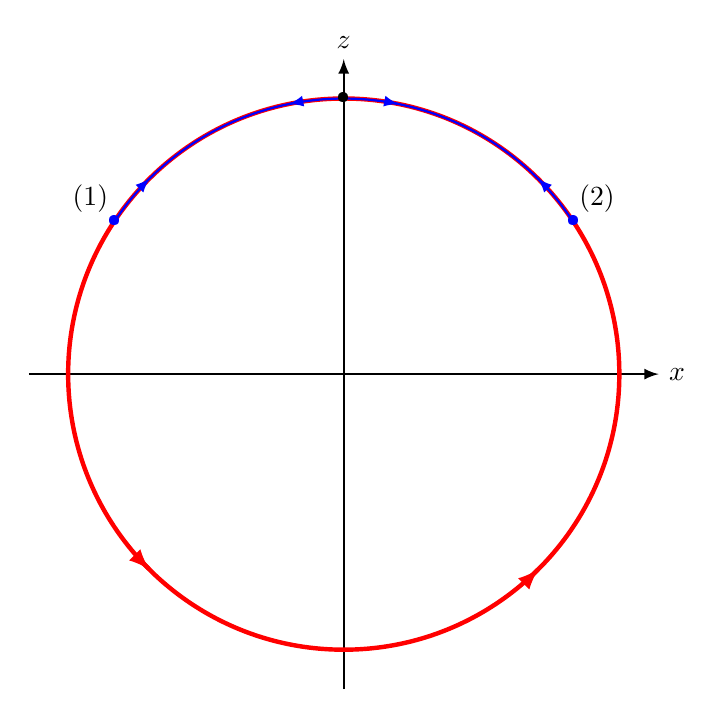
\begin{tikzpicture}
\draw[-latex, thick] ( 0.0, -4) -- (0, 4) node[above]{$z$};
\draw[-latex, thick] (-4,  0) -- (4, 0) node[right]{$x$};

\draw[red, ultra thick] (3.5, 0) arc (0:360:3.5);
\draw[-latex, red, ultra thick] (2.4648737348, -2.4848737348) -- (2.4748737348, - 2.4748737348);
\draw[-latex, red, ultra thick] (-2.4748737348, -2.4748737348) -- (-2.4648737348, -2.4848737348);

\draw[domain=33.540844097:146.459155903,smooth,variable=\x,blue, thick] plot ({3.5 * cos(\x)},{3.5 * sin(\x)});
\draw[-latex, blue, thick] (0.6853426578, 3.4322601227) -- (0.6953426578, 3.4302330223);
\draw[-latex, blue, thick] (2.4748737348,  2.4748737348) -- (2.4648737348, 2.4848737348);
\draw[-latex, blue, thick] (-0.6853426578, 3.4322601227) -- (-0.6953426578, 3.4302330223);
\draw[-latex, blue, thick] (-2.4748737348,  2.4748737348) -- (-2.4648737348, 2.4848737348);

%nodes:
\node[black] at (0, 3.5) {\textbullet};
\node[blue] at (-2.9172225397, 1.9338595227) {\textbullet};
\node[black] at (-2.9172225397 - 0.3, 1.9338595227 + 0.3) {(1)};
\node[blue] at (2.9172225397, 1.9338595227) {\textbullet};
\node[black] at (2.9172225397 + 0.3, 1.9338595227 + 0.3) {(2)};


\end{tikzpicture}
\caption{$\hat{h}(k)$ plotted as function of $k$. The angle with respect to the $z$ axis is given by $\tan(\theta_k) = \Delta^{11}_k/\varepsilon_k$.  In blue: $\mu > 0$. The blue curve starts on the north pole, at the black dot. It then goes counterclockwise until it reaches the point (1). It turns around, goes clockwise until it reaches (2). Finally it returns to the north pole. The total winding number is $w = 0$. In red: $\mu < 0$. The red curve starts and ends at the north pole, at the black dot. It goes counterclockwise around 0. The total winding number is $w = -1$. }
\label{fig.hhatplot}
\end{figure}

We now return to the system at hand. We have $h_z(k) = \varepsilon_k$ and $h_x(k) = \Delta^{11}_k$. If we let $\theta_k$ denote the angle of $\hat{h}(k)$ with the $z$-axis, the winding number is:
\begin{equation}
w = \frac{1}{2\pi}\oint d\theta_k.
\label{eq.definition.windingnumber}
\end{equation} 
The angle $\theta_k$ is given by: $\tan(\theta_k) = \frac{h_x(k)}{h_z(k)} = \frac{\Delta^{11}_k}{\varepsilon_k}$. In turn $\theta_k(c) = \arctan\left(\frac{\Delta^{11}_k}{\varepsilon_k}\right) + c$ for some constant $c$. Calculating $d\theta_k = dk \cdot \partial_k \theta_k$ then gives:
\begin{equation}
w = \frac{1}{2\pi}\int dk \frac{\varepsilon_k\partial_k\Delta^{11}_k - \Delta^{11}_k\partial_k\varepsilon_k}{\varepsilon^2_k + (\Delta^{11}_k)^2} = 2\text{CS}_{1,1}(\Delta^{12}_k = 0). \nonumber
\end{equation} 
Hence, we see that for the separated wires, the Chern-Simons invariant for wire 1 is simply twice the winding of $\hat{h}$ around $\mathbf{h} = 0$. We can hereby very directly understand, why the Chern-Simons invariant is in fact a topological invariant, at least for the separated wires. We have depicted the winding of $\hat{h}(k)$ in figure \ref{fig.hhatplot}. Here we assume, that $\Delta^{11}_k$ is negative for $k < 0$ and positive for $k > 0$. 

\subsection{Edge states: approximate solutions}
\label{subsec.2wiresedgestates}
In this section we come with an approximate analytical solution for the edge states for the separated wires. This is done for a later discussion on their properties. The analysis is largely based on \cite[pp. 196-198]{BernevigTITSC}. 

\begin{figure}
\center
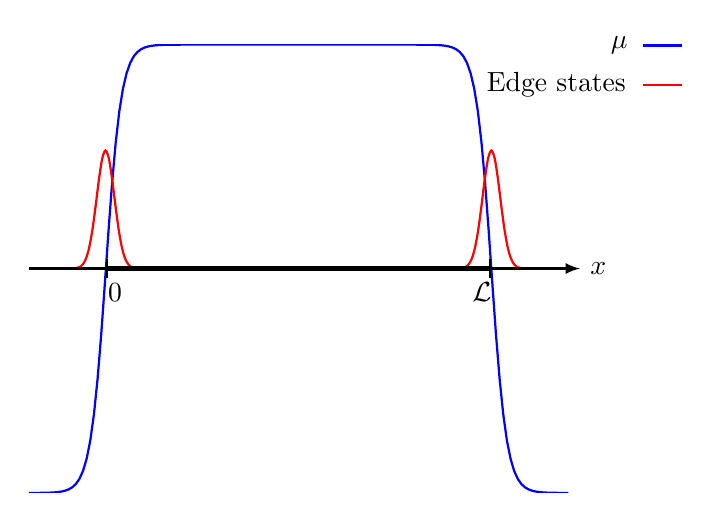
\begin{tikzpicture}
\begin{axis}[samples=150, xtick=\empty, ytick=\empty, axis line style={draw=none}, 
    xmin=-1, xmax=6,
    ymin = -1/2, ymax = 1/2,
    axis lines=center,
    domain=-1:6,
    ]

    \addplot [mark=none,draw=blue, thick] {1/2 * (tanh(5 * \x) - tanh(5 * (\x - 5) ) - 1)};
\end{axis}


\draw[scale=0.5,domain=-1:1,smooth,variable=\x,red, thick] plot ({\x + 0.975 * 2},{ 2 * 2.85 + 3 * exp{- 10 * \x*\x}});
\draw[scale=0.5,domain=-1:1,smooth,variable=\x,red, thick] plot ({\x + 5.875 * 2},{ 2 * 2.85 + 3 * exp{- 10 * \x*\x}});

\node at (0.975 + 0.12, 2.85 - 0.3) {$0$};
\node at (5.875-0.12, 2.85 - 0.3) {$\mathcal{L}$};
\draw[-latex, thick ] (0,2.85) -- (7,2.85) node[right]{$x$};
\draw[-, ultra thick ] (0.975,2.85) -- (5.875,2.85);
\draw[|-, thick ] (0.975,2.85) -- (1,2.85);
\draw[-, ultra thick ] (0.975,2.85) -- (5.875,2.85);
\draw[-|, thick ] (5.7,2.85) -- (5.875,2.85);

\coordinate (a) at (7.8, 5.682);
\coordinate (anode) at (7.5, 5.682);
\coordinate (b) at (8.3, 5.682);
\coordinate (c) at (7.8, 5.182);
\coordinate (d) at (8.3, 5.182);
\coordinate (cnode) at (6.7, 5.182);

\draw[-, thick, blue] (a) -- (b);
\node at (anode) {$\mu$}; 
\draw[-, thick, red] (c) -- (d);
\node at (cnode) {Edge states}; 
\end{tikzpicture}
\caption{Red: Edge states. Blue: chemical potential $\mu = \mu(x)$. Due to the spatial variation of the chemical potential the fermions are confined to the interval between $x = 0$ and $x = \mathcal{L}$. The separated wires are topological for $\mu > 0$. For $\mu < 0$ they are trivial. Hence, edge states form around $\mu = 0$ at $x = 0$ and $x = \mathcal{L}$. }
\label{fig.edgestatesmux}
\end{figure}

We would like to describe the Hamiltonian in real space, because we now ask whether certain states exist at the ends of the wires. To do this we define the operator $\Delta^{11}(p)$ as a function of the momentum operator $p = -i\partial_x$ in the following manner:
\begin{equation}
\Delta^{11}(p)\text{e}^{ikx} = \Delta^{11}_k\text{e}^{ikx}.
\label{eq.Deltapdef}
\end{equation}
Hence, we replace the variable dependency of $k$ in $\Delta^{11}_k$ with an operator dependency on $p$ in $\Delta^{11}(p)$. With this definition we get the Hamiltonian in real space:
\begin{equation}
H_{FF} = \frac{1}{2}\int dx\; \Psi^\dagger_{F}(x) \mathcal{H}_{FF}(x) \Psi_{F}(x), \hspace{0.5cm} \Psi_{F}(x) = \begin{bmatrix} \psi_{1,F}(x) & \psi^\dagger_{1,F}(x) & \psi_{2,F}(x) & \psi^\dagger_{2,F}(x)\end{bmatrix}^t
\label{eq.2wiresMFHamiltonianrealspace}
\end{equation}
With the real space Hamiltonian kernel:
\begin{equation}
\mathcal{H}_{FF}(x) = \begin{bmatrix} 
\frac{p^2}{2m_F} - \mu & \Delta^{11}(p) & 0 & 0 \\
\Delta^{11}(p) & -\left(\frac{p^2}{2m_F} - \mu \right) & 0 & 0 \\
0 & 0 & \frac{p^2}{2m_F} - \mu & -\Delta^{11}(p) \\
0 & 0 & -\Delta^{11}(p) & -\left(\frac{p^2}{2m_F} - \mu \right)
\end{bmatrix}.
\label{eq.2wiresMFHamiltonianrealspacefirstquantization}
\end{equation}
For the sake of clarity let us see how e.g. the term $\Delta^{11}_kc_{1,-k}c_{1,k}$ appears from this expression:
\begin{align}
\int dx \; \psi_{1,F}(x) \Delta^{11}(p) \psi_{1,F}(x) &= \frac{1}{\mathcal{L}}\sum_{k,q}c_{1,k} c_{1,q}\int dx \; \text{e}^{ikx}\Delta^{11}(p)\text{e}^{iqx} = \frac{1}{\mathcal{L}}\sum_{k,q}\Delta^{11}_qc_{1,k}c_{1,q}\int dx \; \text{e}^{i(k + q)x} \nonumber \\
&= \sum_{k}\Delta^{11}_kc_{1,-k}c_{1,k}, \nonumber 
\end{align}
since $\int dx\; \text{e}^{i(k + q)x} =\mathcal{L} \delta_{k,-q} $. Here we use the Fourier decomposition $\psi_{1,F}(x) = \frac{1}{\sqrt{L}}\sum_k\text{e}^{ikx}c_{1,k}$. Now we form junctions of topogically distinct phases by changing the sign of $\mu$ at $x = 0$ and $x = \mathcal{L}$. Hence, we let $\mu = \mu(x)$ as shown in figure \ref{fig.edgestatesmux}. Due to the spatial variation of the chemical potential the fermions are confined to the wire between $x = 0$ and $x = \mathcal{L}$. In first quantization we find solutions by solving $\mathcal{H}(x)\psi(x) = E\psi(x)$. The edge states are zero energy modes, so we solve for $E = 0$. We assume, that $\mu(x)$ varies slowly over the interparticle length scale $1/k_F$. When this is fulfilled the solution $\psi(x)$ will also vary slowly and hence the curvature of $\psi(x)$ proportional to $p^2\psi(x)$ is negligible. This means, that to a good approximation we only keep the operator $p$ up to first order. In the numerical analysis we will see, that $\Delta^{11}_k$ is linear in $k$ for $k/k_F \ll 1$. This means, that $\Delta^{11}(p)$ is linear in $p$, when $p/k_F$ used on a state is small. Hence, we ignore $p^2/2m_F$ and let $\Delta^{11}(p) = \Delta^{11} \cdot \tilde{p}$, with $\Delta^{11} = k_F\left.\frac{\partial \Delta^{11}_k}{\partial k}\right|_{k=0}$ and $\tilde{p} = p/k_F$. We assume $\Delta^{11} > 0$. We take the ansatz:
\begin{equation}
\psi^{i}_1(x) = \exp\left(-\frac{k_F}{\Delta^{11}}\int_{0}^{x} dx'\; \mu(x') \right)\mathbf{u}^{i}_{1}, \hspace{0.5cm} \psi^{i}_2(x) = \exp\left(+\frac{k_F}{\Delta^{11}}\int_{\mathcal{L}}^{x} dx'\; \mu(x') \right)\mathbf{u}^{i}_{2}, \nonumber
\end{equation}  
The superscript ${}^i$ refers to the wire, the subscript ${}_j$ to which end the wave function is located. Since $\Delta^{11}$ is in units of energy the exponents are unitless. Since $\Delta^{11} > 0$, we see that these states are exponentially localized at the edges. From this we get eigenvalue equations for $\mathbf{u}^{i}_{j}$. Defining $g_1(x) = \frac{1}{N}\text{e}^{-\frac{k_F}{\Delta^{11}}\int_{0}^{x} dx' \mu(x')}$, $g_2(x) = \frac{1}{N}\text{e}^{+\frac{k_F}{\Delta^{11}}\int_{\mathcal{L}}^{x} dx' \mu(x')}$ and $N^2 = \int dx |g_j(x)|^2$ a normalization constant we hereby get the approximate solutions:
\begin{align}
\psi^1_1(x) &= g_1(x)\frac{\text{e}^{+i\pi/4}}{\sqrt{2}}\begin{bmatrix} 1 & -i & 0 & 0 \end{bmatrix}^t , \hspace{0.5cm} \psi^1_2(x) = g_2(x)\frac{\text{e}^{-i\pi/4}}{\sqrt{2}}\begin{bmatrix} 1 & +i & 0 & 0 \end{bmatrix}^t, \nonumber \\
\psi^2_1(x) &= g_1(x)\frac{\text{e}^{-i\pi/4}}{\sqrt{2}}\begin{bmatrix} 0 & 0 & 1 & +i \end{bmatrix}^t , \hspace{0.5cm} \psi^2_2(x) = g_2(x)\frac{\text{e}^{+i\pi/4}}{\sqrt{2}}\begin{bmatrix} 0 & 0 & 1 & -i \end{bmatrix}^t.
\end{align}
From equation \eqref{eq.2wiresTminuswireexchangefirstquantization} we have, that the time reversal operator that squares to minus the identity is given by: $\mathcal{T}_- = i\sigma_2\otimes\tau_0 \cdot K$. We hereby get: $\mathcal{T}_-\psi^1_1(x) = -\psi^2_1(x), \mathcal{T}_-\psi^1_2(x) = -\psi^2_2(x)$. The edge states at the same end in each wire are therefore Kramers partners. This is crucial for the following analysis. For sake of completeness let us write up the second quantized version of the four states. The eigenstates define the diagonalisation matrix $U(x) = \begin{bmatrix} \psi^{1}_{1}(x) & \psi^{1}_{2}(x) & \psi^{2}_{1}(x) & \psi^{2}_{2}(x) \end{bmatrix}$. This has the unitarity property, that $\int dx \; U^\dagger(x) U(x) = \mathbb{I}$. We then let the operators $\gamma^{j}_{0,1}, \gamma^{j}_{0,2}$ for wire $j$ be given by:
\begin{equation}
\begin{bmatrix} \psi_{1,F}(x) \\ \psi_{1,F}^\dagger(x) \\ \psi_{2,F}(x) \\ \psi_{2,F}^\dagger(x) \end{bmatrix} = U(x) \begin{bmatrix} \gamma^{1}_{0,1} \\ \gamma^{1}_{0,2} \\ \gamma^{2}_{0,1} \\ \gamma^{2}_{0,2} \end{bmatrix} \Rightarrow \begin{bmatrix} \gamma^{1}_{0,1} \\ \gamma^{1}_{0,2} \\ \gamma^{2}_{0,1} \\ \gamma^{2}_{0,2} \end{bmatrix} = \int dx \; U^\dagger(x) \begin{bmatrix} \psi_{1,F}(x) \\ \psi_{1,F}^\dagger(x) \\ \psi_{2,F}(x) \\ \psi_{2,F}^\dagger(x) \end{bmatrix}.
\label{eq.Majoranaedgemodedef} 
\end{equation} 
Written out these operators are: 
\begin{align}
\gamma^1_{0,1} &= \int dx \; g_1(x)\frac{\text{e}^{-i\pi/4}}{\sqrt{2}}(\psi_{1,F}(x) + i\psi^\dagger_{1,F}(x)), \hspace{0.5cm} \gamma^1_{0,2} = \int dx \; g_2(x)\frac{\text{e}^{+i\pi/4}}{\sqrt{2}}(\psi_{1,F}(x) - i\psi^\dagger_{1,F}(x)), \nonumber \\
\gamma^2_{0,1} &= \int dx \; g_1(x)\frac{\text{e}^{+i\pi/4}}{\sqrt{2}}(\psi_{2,F}(x) - i\psi^\dagger_{2,F}(x)), \hspace{0.5cm} \gamma^2_{0,2} = \int dx \; g_2(x)\frac{\text{e}^{-i\pi/4}}{\sqrt{2}}(\psi_{2,F}(x) + i \psi^\dagger_{2,F}(x)). \nonumber 
\end{align}
In this manner $\psi^{i}_{j}(x)$ and $\gamma^{i}_{0,j}\ket{\text{S}}_0$ are equivalent. These operators are special in the sense, that they are their own antiparticle: $\left(\gamma^{i}_{0,j}\right)^\dagger = \gamma_{0,j}$.\footnote{This also illuminates why we chose the rather arbitrary phase factors $\text{e}^{\pm i\pi/4}$. Had we \textit{not} done this, there would be some phase difference between $\left(\gamma^{i}_{0,j}\right)^\dagger$ and $\gamma^{i}_{0,j}$.} Such a fermionic particle is called a Majorana mode in condensed matter physics. Besides being their own antiparticle, they have to obey the modified anticommutator relation:
\begin{equation}
\{\gamma^{i_1}_{0,j_1}, \gamma^{i_2}_{0,j_2} \} = \delta_{i_1,i_2}\delta_{j_1,j_2}. \nonumber
\end{equation}
This is explicitly verified to be the case for the above operators.\footnote{Often one also meets the requirement, that the anticommutator equals $2\delta_{i_1,i_2}\delta_{j_1,j_2}$. This is simply a matter of convention.} From this we can form regular but highly nonlocal fermionic operators: $d_j = \frac{1}{\sqrt{2}}(\gamma^{j}_{0,1} + i\gamma^{j}_{0,2})$. The key result of this section is thus, that $\ket{\text{S}}_0$ and $d_j^\dagger\ket{\text{S}}_0$ are degenerate ground states of the system. The topologically non-trivial state is therefore characterized by the presence of \textit{one} more particle than the trivial one, which is exponentially located on the edges.\footnote{In the literature one also meets the notion of a Majorana mode at each end, hence two in total. However, since $\gamma^\dagger_0\gamma_0 = \gamma_0^2 = \frac{1}{2}$ for Majorana operators, we cannot count them. Hence, the notion of a specific number of Majorana modes is undefined.}

In second quantization the above notion of Kramers partners is described by the fact, that: $T_-\gamma^1_{0,j}T_-^{-1} = \gamma^2_{0,j}$, simply because $\psi_{1,F}(x) \overset{T_-}{\to} \psi_{2,F}(x)$ and $T_-$ is antiunitary.

\section{Kramers degeneracy: protection of edge states}
\label{sec.2wireskramersdegeneracy}
In this section we show, that the interwire interaction protects the edge states as long as no interwire mean field has formed. We show, that this is because Kramers partners do not couple.

Consider a general system described by the Hamiltonian $H$. Assume, that this Hamiltonian is time reversal invariant, $[T, H] = 0$, and that $T^2 = -\mathbb{I}$. Let $\ket{\psi_1}$ and $\ket{\psi_2}$ be eigenstates to the Hamiltonian, with energy $E_1$ and $E_2$, and Kramers partners: $\ket{\psi_2} = T\ket{\psi_1}$. Since $[T, H] = 0$ the two states have the same energy: 
\begin{equation}
E_2\ket{\psi_2} = HT\ket{\psi_1} = TH\ket{\psi_1} = E_1\ket{\psi_2}. \nonumber
\end{equation}
So $E_2 = E_1$. Further, the states are orthogonal:
\begin{equation}
\braket{\psi_1|\psi_2} = \braket{T\psi_2|T\psi_1} = \braket{-\psi_1|\psi_2} = -\braket{\psi_1|\psi_2} \Rightarrow \braket{\psi_1|\psi_2} = 0. \nonumber  
\end{equation}
In the first equality we use, that we can flip the inner product by going to the time reversed states \cite[p. 274]{Sakurai}. In the second equality we use, that $T\ket{\psi_2} = -\ket{\psi_1}$, since $T^2 = -\mathbb{I}$. Hence, any energy state in a time reversal invariant system with $T^2 = -\mathbb{I}$ is twofold degenerate. This is Kramers degeneracy. Now let $H'$ be a perturbation to the Hamiltonian, which respects the time reversal symmetry: $[T, H'] = 0$. In degenerate perturbation theory we calculate the matrix with entries $W_{ij} = \bra{\psi_i}H'\ket{\psi_j}$. The eigenstates of $H$ remain good eigenstates if the states uncouple: $\bra{\psi_1}H'\ket{\psi_2} = 0$, so that $W_{ij}$ is diagonal. This is exactly the case for Kramers partners: 
\begin{equation}
\bra{\psi_1}H'\ket{\psi_2} = \bra{T\psi_2}TH'T^{-1}\ket{T\psi_1} = \bra{T\psi_2}H'\ket{T\psi_1} = -\bra{\psi_1}H'\ket{\psi_2} \Rightarrow \bra{\psi_1}H'\ket{\psi_2} = 0. \nonumber
\end{equation}
The first equality holds, since $H'$ is hermitian \cite[p. 274]{Sakurai}. 

Now what has this to do with the system at hand? We let $\ket{\psi_{i}^{j}} = \gamma_{i,0}^{j}\ket{\text{S}}_0$ for $i, j = 1, 2$. In this way, $\ket{\psi_{1}^1}$ is the edge state in wire 1 at end 1, $\ket{\psi_{2}^1}$ in wire 1 at end 2, and so forth. From above we know, that the edge states at end $i$, $\ket{\psi_{i}^1}$ and $\ket{\psi_{i}^2}$, are Kramers partners. If we can show, that the interwire interaction $H' = H^\text{int}_{FF,12}$ is time reversal invariant under $T_-$, then the above analysis shows that the edge states at the same end of the wire cannot couple. From equation \eqref{eq.Hint12realspace} we have:
\begin{equation}
H^\text{int}_{FF,12} = \int dx_1 dx_2 \psi^\dagger_{1,F}(x_1)\psi^\dagger_{2,F}(x_2) \tilde{V}_{\text{ind}}^{12}(x_1-x_2,0) \psi_{2,F}(x_2)\psi_{1,F}(x_1),
\end{equation}
with $\tilde{V}_{\text{ind}}^{12}(x_1-x_2,0)$ the zero frequency induced interaction in real space. Now $T_-\psi_{1,F}(x)T^{-1}_- = \psi_{2,F}(x)$ and $T_-\psi_{2,F}(x)T^{-1}_- = -\psi_{1,F}(x)$. Finally, $\tilde{V}_{\text{ind}}^{12}(x, 0)$ is real, so we get that $T_-H^\text{int}_{FF,12}T_-^{-1} = H^\text{int}_{FF,12}$. Hence, the edge states at the same end of the wire cannot couple. Further, the edge states at opposite ends of the wire are macroscopically separated. Therefore, these cannot couple either. In conclusion, the edge state in each wire is protected, as long as the interwire interaction is a perturbation to the system, which is to say no interwire mean field has formed.  

\section{Qualitative understanding of cross over}
\label{sec.2wirestransitionqualitative}
In this section we come with a qualitative analysis of how the cross over from $p$- to $s$-wave occures using the previous two sections. 

\textbf{Imaginary interwire pairing}: Assume that as the wires are brought closer together, the system chooses the interwire pairing to be \textit{imaginary}. Then the system \textit{breaks} the time reversal symmetry $T_-$. In this case there is no longer a Kramers degeneracy. As a consequence the edge states can couple and gap away. We can actually calculate by how much the edge states gap. In this connection we define the operator $\Delta^{12}(p)$ as: $\Delta^{12}(p)\text{e}^{ikx} = \Delta^{12}_k\text{e}^{ikx}$. Since $\Delta^{12}_k$ is even in $k$, there is no first order term in $k$. Hence for states with small curvatures like the edge states we can approximate $\Delta^{12}(p) = \Delta^{12}_{k=0}$. This means, that the perturbation in real space relevant for the edge states is:
\begin{equation}
\mathcal{H}'_{FF}(x) = \Delta^{12}_{k=0}\begin{bmatrix} 
0 & 0 &  0 & -i \\
0 & 0 & -i & 0 \\
0 & i & 0  & 0 \\
i & 0 & 0  & 0  \end{bmatrix}
\label{eq.interwirepairingrealspace}
\end{equation}
The edge states in wires 1 and 2 in first quantization are described by the wave functions $\psi^1_1, \psi^2_1, \psi^1_2, \psi^2_2$ found in subsection \ref{subsec.2wiresedgestates}. With this as an ordered basis we can calculate the perturbation matrix $W$ with entries $\bra{\psi^{i}_j}\mathcal{H}'\ket{\psi^{l}_k}$. We get:
\begin{equation}
W = \Delta^{12}_{k=0} \begin{bmatrix} 
0 & 0 & -i &  0 \\
0 & 0 &  0 & -i \\
i & 0 &  0 & 0 \\
0 & i &  0 & 0 \end{bmatrix} \nonumber
\end{equation}  
There are also couplings between the edge state at one end in wire 1 with the edge state at the other end in wire 2 and vice versa. This coupling is proportional to $\int dx \; g_1(x)g_2(x)$ and is therefore exponentially suppressed by the length of the wire. Hence, it is negligible for a macroscopic system. In this sense the only nonzero couplings are between the edge states at the same end in each wire. The shift in energies are the eigenvalues of $W$. These along with the corresponding perturbed wave functions are then given by:
\begin{align}
E &= +\Delta^{12}_{k=0}, \hspace{0.5cm} \frac{1}{\sqrt{2}}\left( \psi^1_j(x) + i\psi^2_j(x) \right), \nonumber \\
E &= -\Delta^{12}_{k=0}, \hspace{0.5cm} \frac{1}{\sqrt{2}}\left(\psi^1_j(x) - i\psi^2_j(x) \right),
\label{eq.perturbededgestates}
\end{align}
for the edge at $x = 0$ and $x = \mathcal{L}$ indicated by $j = 1$ and $j = 2$ respectively. Hence, the interwire pairing couples the two edge states in each wire around $x = 0$ and the two edge states around $x = \mathcal{L}$. This makes it explicit, how the states are gapped! This is the content of figure \ref{fig.2wiresedgestates} going from the top center to the middle left. 

\textbf{Real interwire pairing}: Assume that as the wires are brought closer together, the system chooses the interwire pairing to be \textit{real}. In this situation the system still respects the time reversal symmetry $T_-$. Kramers degeneracy is still present and therefore any energy state must be twofold degenerate. Further, since the system has a particle-hole symmetry the energy spectrum is symmetric around $E = 0$ (relative to the ground state). Therefore the zero energy edge states are locked as long as the bulk energy gap remains open. A direct calculation of the first order energy shift performed in the same way as in the above verifies this explicitly. The bulk energy dispersions in this situation are given by: $E^{\pm}_{F,k} = \sqrt{\varepsilon^2_k + (\Delta^{11}_k \pm \Delta^{12}_k)^2}$. The bulk gap will therefore eventually close as we bring the wires closer together. This happens exactly when $|\Delta^{12}_{k_0}| = |\Delta^{11}_{k_0}|$, where $\pm k_0$ are the Fermi points given by: $\varepsilon_{\pm k_0} = 0$. Hence, we expect a topological phase transition in this situation, with a topologically non-trivial system for $|\Delta^{12}_{k_0}| < |\Delta^{11}_{k_0}|$ and topologically trivial for $|\Delta^{12}_{k_0}| > |\Delta^{11}_{k_0}|$. This is the content of figure \ref{fig.2wiresedgestates} going from the top center to the middle and bottom right. 

\begin{figure}
\center
\begin{tikzpicture}
\draw[|-latex, thick] (0, 0) -- (0,  2) node[above]{$E$};
\draw[-, thick]   (0, 0) -- (0, -2);
\node at (-0.4, 0) {$0$};

\draw[-, dashed] (0, 1)--(2, 1);
\draw[-, thick] (-0.1, 1)--(0.1, 1);
\node at (-0.7,1) {$E_{F,k_0}$};

\draw[-, dashed] (0,    -1) -- (2,   -1);
\draw[-, thick]  (-0.1, -1) -- (0.1, -1);
\node at (-0.85,-1) {$-E_{F,k_0}$};

\draw[-, ultra thick] (1, 1)--(1, 2);
\draw[-, ultra thick] (1, -1)--(1, -2);
\node[red] at (1, 0) {\textbullet};

\draw[-, ultra thick] (2, 1)--(2, 2);
\draw[-, ultra thick] (2, -1)--(2, -2);
\node[blue] at (2, 0) {\textbullet};

\draw[-, dashed] (0,0.01) -- (2,0.01);

\node at (3, -1.9) {$0$};
\node at (5, -1.9) {$\mathcal{L}$};

\draw[scale=0.5,domain=-1:1,smooth,variable=\x,red] plot ({\x + 6},{ 2 * exp{- 15 * \x*\x} - 3});
\draw[scale=0.5,domain=-1:1,smooth,variable=\x,red] plot ({\x + 10},{ 2 * exp{- 15 * \x*\x} -3});
\draw[|-latex, thick ] (3,-1.5) -- (5.8,-1.5) node[right]{$x$};
\draw[-, ultra thick ] (3,-1.5) -- (5,-1.5);

\node at (3, 1.1) {$0$};
\node at (5, 1.1) {$\mathcal{L}$};

\draw[scale=0.5,domain=-1:1,smooth,variable=\x,blue] plot ({\x + 6},{ 2 * exp{- 15 * \x*\x} + 3});
\draw[scale=0.5,domain=-1:1,smooth,variable=\x,blue] plot ({\x + 10},{ 2 * exp{- 15 * \x*\x} + 3});

\draw[|-latex, thick ] (3,1.5) -- (5.8,1.5) node[right]{$x$};
\draw[-, ultra thick] (3, 1.5) -- (5, 1.5);

%\draw[-, dashed] (5.8, -1.5) -- (5.8, 1.5);
\node at (2.2, 2.8) {$\Delta^{12}_k = 0$};

%%%%%%%%%%%%%%%%%%%%%%%%%%%%%%%%%%%
\pgfmathsetmacro{\hmove}{-4}
\pgfmathsetmacro{\vmove}{-6}

\draw[|-latex, thick] (\hmove, \vmove) -- (\hmove,  2 + \vmove) node[above]{$E$};
\draw[-, thick]   (\hmove, \vmove) -- (\hmove, -2 + \vmove);
\node at (-0.4 + \hmove, 0 + \vmove) {$0$};

\draw[-, dashed] (0 + \hmove, 1 + \vmove)--(2 + \hmove, 1 + \vmove);
\draw[-, thick] (-0.1 + \hmove, 1 + \vmove)--(0.1 + \hmove, 1 + \vmove);
\node at (-0.7 + \hmove, 1 + \vmove) {$E_{F,k_0}$};

\draw[-, dashed] (0 + \hmove,    -1 + \vmove) -- (2 + \hmove,   -1 + \vmove);
\draw[-, thick]  (-0.1 + \hmove, -1 + \vmove) -- (0.1 + \hmove, -1 + \vmove);
\node at (-0.85 + \hmove,-1 + \vmove) {$-E_{F,k_0}$};

\draw[-, ultra thick] (1 + \hmove, 1 + \vmove)--(1 + \hmove, 2 + \vmove);
\draw[-, ultra thick] (1 + \hmove, -1 + \vmove)--(1 + \hmove, -2 + \vmove);

%gapped edge state:
\coordinate (edge1energy) at (1 + \hmove, 0.5 + \vmove);
\node[right=0.0cm of edge1energy] {$+\Delta^{12}_{k=0}$}; 
\draw[-latex, semithick] (1 + \hmove, 0 + \vmove)--(1 + \hmove, 0.5 + \vmove);
\node[red] at (edge1energy) {\textbullet};

\draw[-, ultra thick] (2 + \hmove, 1 + \vmove)--(2 + \hmove, 2 + \vmove);
\draw[-, ultra thick] (2 + \hmove, -1 + \vmove)--(2 + \hmove, -2 + \vmove);

%gapped edge state:
\coordinate (edge2energy) at (2 + \hmove, -0.5 + \vmove);
\node[right=0.0cm of edge2energy] {$-\Delta^{12}_{k=0}$}; 
\draw[-latex, semithick] (2 + \hmove, 0 + \vmove)--(2 + \hmove, -0.5 + \vmove);
\node[blue] at (edge2energy) {\textbullet};

\draw[-, dashed] (0 + \hmove,0.01 + \vmove) -- (2 + \hmove,0.01 + \vmove);

\node at (3 + \hmove, -1.4 + \vmove) {$0$};
\node at (5 + \hmove, -1.4 + \vmove) {$\mathcal{L}$};

\draw[|-latex, thick ] (3 + \hmove,-1.0 + \vmove) -- (5.8 + \hmove,-1.0 + \vmove) node[right]{$x$};
\draw[-, ultra thick ] (3 + \hmove,-1.0 + \vmove) -- (5 + \hmove,-1.0 + \vmove);

\node at (3 + \hmove, 0.6 + \vmove) {$0$};
\node at (5 + \hmove, 0.6 + \vmove) {$\mathcal{L}$};

\draw[|-latex, thick ] (3 + \hmove, 1.0 + \vmove) -- (5.8 + \hmove,1.0 + \vmove) node[right]{$x$};
\draw[-, ultra thick] (3 + \hmove, 1.0 + \vmove) -- (5 + \hmove, 1.0 + \vmove);

\node at (2.2 + \hmove, 2.8 + \vmove) {$\Delta^{12}_k \neq 0$, imaginary};

%%%%%%%%%%%%%%%%%%%%%%%%%%%%%%%%%%%
\pgfmathsetmacro{\hmove}{4}
\pgfmathsetmacro{\vmove}{-6}
\pgfmathsetmacro{\Eminchange}{0.4}

\draw[|-latex, thick] (\hmove, \vmove) -- (\hmove,  2 + \vmove) node[above]{$E$};
\draw[-, thick]   (\hmove, \vmove) -- (\hmove, -2 + \vmove);
\node at (-0.4 + \hmove, 0 + \vmove) {$0$};

\draw[-, dashed] (0 + \hmove, 1 - \Eminchange + \vmove)--(2 + \hmove, 1 - \Eminchange + \vmove);
\draw[-, thick] (-0.1 + \hmove, 1 - \Eminchange + \vmove)--(0.1 + \hmove, 1 - \Eminchange + \vmove);
\node at (-0.7 + \hmove, 1 - \Eminchange + \vmove) {$E_{F,k_0}$};

\draw[-, dashed] (0 + \hmove,    -1 + \Eminchange + \vmove) -- (2 + \hmove,   -1 + \Eminchange + \vmove);
\draw[-, thick]  (-0.1 + \hmove, -1 + \Eminchange + \vmove) -- (0.1 + \hmove, -1 + \Eminchange + \vmove);
\node at (-0.85 + \hmove, -1 + \Eminchange + \vmove) {$-E_{F,k_0}$};

\draw[-, ultra thick] (1 + \hmove, 1 - \Eminchange + \vmove)--(1 + \hmove, 2 + \vmove);
\draw[-, ultra thick] (1 + \hmove, -1 + \Eminchange + \vmove)--(1 + \hmove, -2 + \vmove);
\node[red] at (1 + \hmove, 0 + \vmove) {\textbullet};

\draw[-, ultra thick] (2 + \hmove, 1 - \Eminchange + \vmove)--(2 + \hmove, 2 + \vmove);
\draw[-, ultra thick] (2 + \hmove, -1 + \Eminchange + \vmove)--(2 + \hmove, -2 + \vmove);
\node[blue] at (2 + \hmove, 0 + \vmove) {\textbullet};

\draw[-, dashed] (0 + \hmove, 0.01 + \vmove) -- (2 + \hmove, 0.01 + \vmove);

\node at (3 + \hmove, -1.4 + \vmove) {$0$};
\node at (5 + \hmove, -1.4 + \vmove) {$\mathcal{L}$};

\draw[scale=0.5,domain=-1:1,smooth,variable=\x,red] plot ({\x + 6 + 2*\hmove},{ 2 * exp{- 15 * \x*\x} - 2.0 + 2*\vmove});
\draw[scale=0.5,domain=-1:1,smooth,variable=\x,blue] plot ({\x + 10 + 2*\hmove},{ 2 * exp{- 15 * \x*\x} -2.0 + 2*\vmove});
\draw[|-latex, thick ] (3 + \hmove,-1.0 + \vmove) -- (5.8 + \hmove,-1.0 + \vmove) node[right]{$x$};
\draw[-, ultra thick ] (3 + \hmove,-1.0 + \vmove) -- (5 + \hmove,-1.0 + \vmove);

\node at (3 + \hmove, 0.6 + \vmove) {$0$};
\node at (5 + \hmove, 0.6 + \vmove) {$\mathcal{L}$};

\draw[scale=0.5,domain=-1:1,smooth,variable=\x,red] plot ({\x + 6  + 2*\hmove},{ 2 * exp{- 15 * \x*\x} + 2.0 + 2*\vmove});
\draw[scale=0.5,domain=-1:1,smooth,variable=\x,blue] plot ({\x + 10 + 2*\hmove},{ 2 * exp{- 15 * \x*\x} + 2.0 + 2*\vmove});

\draw[|-latex, thick ] (3 + \hmove,1.0 + \vmove) -- (5.8 + \hmove,1.0 + \vmove) node[right]{$x$};
\draw[-, ultra thick] (3 + \hmove, 1.0 + \vmove) -- (5 + \hmove, 1.0 + \vmove);

\node at (2.2 + \hmove, 2.8 + \vmove) {$|\Delta^{12}_{k_0}| < |\Delta^{11}_{k_0}|$, real};

%squezzing of gap:
\draw[-latex, semithick] (0.5 + \hmove, 1  + \vmove)--(0.5 + \hmove, 1 - \Eminchange + \vmove);
\draw[-latex, semithick] (0.5 + \hmove, -1 + \vmove)--(0.5 + \hmove, -1 + \Eminchange + \vmove);

%%%%%%%%%%%%%%%%%%%%%%%%%%%%%%%%%%%
\pgfmathsetmacro{\hmove}{4}
\pgfmathsetmacro{\vmove}{-12}
\pgfmathsetmacro{\Eminchange}{0.4}

\draw[|-latex, thick] (\hmove, \vmove) -- (\hmove,  2 + \vmove) node[above]{$E$};
\draw[-, thick]   (\hmove, \vmove) -- (\hmove, -2 + \vmove);
\node at (-0.4 + \hmove, 0 + \vmove) {$0$};

\draw[-, dashed] (0 + \hmove, 1 - \Eminchange + \vmove)--(2 + \hmove, 1 - \Eminchange + \vmove);
\draw[-, thick] (-0.1 + \hmove, 1 - \Eminchange + \vmove)--(0.1 + \hmove, 1 - \Eminchange + \vmove);
\node at (-0.7 + \hmove, 1 - \Eminchange + \vmove) {$E_{F,k_0}$};

\draw[-, dashed] (0 + \hmove,    -1 + \Eminchange + \vmove) -- (2 + \hmove,   -1 + \Eminchange + \vmove);
\draw[-, thick]  (-0.1 + \hmove, -1 + \Eminchange + \vmove) -- (0.1 + \hmove, -1 + \Eminchange + \vmove);
\node at (-0.85 + \hmove, -1 + \Eminchange + \vmove) {$-E_{F,k_0}$};

\draw[-, ultra thick] (1 + \hmove, 1 - \Eminchange + \vmove)--(1 + \hmove, 2 + \vmove);
\draw[-, ultra thick] (1 + \hmove, -1 + \Eminchange + \vmove)--(1 + \hmove, -2 + \vmove);
%\node[red] at (1 + \hmove, 0 + \vmove) {\textbullet};

\draw[-, ultra thick] (2 + \hmove, 1 - \Eminchange + \vmove)--(2 + \hmove, 2 + \vmove);
\draw[-, ultra thick] (2 + \hmove, -1 + \Eminchange + \vmove)--(2 + \hmove, -2 + \vmove);
%\node[blue] at (2 + \hmove, 0 + \vmove) {\textbullet};

\draw[-, dashed] (0 + \hmove, 0.01 + \vmove) -- (2 + \hmove, 0.01 + \vmove);

\node at (3 + \hmove, -0.9 + \vmove) {$0$};
\node at (5 + \hmove, -0.9 + \vmove) {$\mathcal{L}$};

\draw[|-latex, thick ] (3 + \hmove,-0.5 + \vmove) -- (5.8 + \hmove,-0.5 + \vmove) node[right]{$x$};
\draw[-, ultra thick ] (3 + \hmove,-0.5 + \vmove) -- (5 + \hmove,  -0.5 + \vmove);

\node at (3 + \hmove, 0.1 + \vmove) {$0$};
\node at (5 + \hmove, 0.1 + \vmove) {$\mathcal{L}$};

\draw[|-latex, thick ] (3 + \hmove,0.5 + \vmove) -- (5.8 + \hmove,0.5 + \vmove) node[right]{$x$};
\draw[-, ultra thick] (3 + \hmove, 0.5 + \vmove) -- (5 + \hmove,  0.5 + \vmove);

\node at (2.2 + \hmove, 2.8 + \vmove) {$|\Delta^{12}_{k_0}| > |\Delta^{11}_{k_0}|$, real};

%squezzing of gap:
\draw[-latex, semithick] (0.5 + \hmove, 1 - \Eminchange + \vmove)--(0.5 + \hmove, 1  + \vmove);
\draw[-latex, semithick] (0.5 + \hmove, -1 + \Eminchange + \vmove)--(0.5 + \hmove, -1 + \vmove);

\end{tikzpicture}
\caption{\textbf{Top centered}: for $\Delta^{12}_k=0$ we have two copies of the single wire system with the interwire interaction as a perturbation. There are two symmetry-protected edge states, one at each wire and two energy dispersions mirrored in $E = 0$. This is indicated with red and blue dots. $k_0$ is defined by: $0 = \varepsilon_{k_0} = \frac{k^2_0}{2m_F} - \mu$. \textbf{Middle left}: If the system chooses an imaginary interwire pairing the system breaks the $T^2 = -\mathbb{I}$ symmetry. The edge states are therefore no longer protected at $E = 0$, and the edge states are gapped by $2\Delta^{12}_{k=0}$. \textbf{Middle and bottom right}: If the system chooses a real interwire pairing the system still respects the $T^2 = -\mathbb{I}$ symmetry. \textbf{Middle right}: Before an energy gap closing the edge states are still protected. Due to the interwire pairing the two edge states are located equally on each wire in opposite ends. Hence, the colours of the wave functions. The gap is closing; this is indicated by the arrows squezzing the gap. 
\textbf{Bottom right}: After the gap closing the edge states are gone. The system is topologically trivial. The gap is opening again indicated by the arrows.}
\label{fig.2wiresedgestates}
\end{figure}

It turns out that we can find approximate eigenstates for $\Delta^{12}_{k=0} \ll \Delta^{11}$. We take the ansatz $\psi_j^{\pm}(x) = g_j^{\pm}(x)\cdot \mathbf{u}^{\pm}_j$ for four component vectors $\mathbf{u}^{\pm}_j$. Further $g_1^{\pm}(x) = \frac{1}{N}\text{e}^{-\frac{k_F}{\Delta^{11}}\int_0^x dx' \; \left[\mu(x') \pm i\Delta^{12}_{k=0}\right] }$ and $g_2^{\pm}(x) = \frac{1}{N}\text{e}^{+\frac{k_F}{\Delta^{11}}\int_{\mathcal{L}}^x dx' \; \left[\mu(x') \pm i\Delta^{12}_{k=0}\right] }$. We then seach for solutions to $(\mathcal{H}_{FF}(x) + \mathcal{H}'_{FF}(x))\psi_j^{\pm}(x) = 0$, only keeping $p$ up to first order. The first and second derivative ($l = 1$ and $l = 2$) has a term proportional to $\left(\frac{\Delta^{12}_{k=0}}{\Delta^{11}}\right)^l\psi_j^{\pm}(x)$. Since we only keep $p$ up to first order, the second derivative must be small with respect to the first one. It is then clear, that $\left(\frac{\Delta^{12}_{k=0}}{\Delta^{11}}\right)^2 \ll \frac{\Delta^{12}_{k=0}}{\Delta^{11}}$ is required. In turn $\Delta^{12}_{k=0} \ll \Delta^{11}$. As $\Delta^{12}_{k=0}$ comes closer to $\Delta^{11}$ we must add higher order terms in $p$ to get accurate results. With the above ansatz we get the following solutions in the $\Delta^{12}_{k=0} \ll \Delta^{11}$ regime:
\begin{align}
\psi_1^{+}(x) &= \frac{g_1^{+}(x)}{2}\begin{bmatrix} 1 & -i & 1 & i \end{bmatrix}^t, \hspace{0.5cm} \psi_1^{-}(x) = \frac{g_1^{-}(x)}{2}\begin{bmatrix} i & 1 & -i & 1 \end{bmatrix}^t, \nonumber \\
\psi_2^{+}(x) &= \frac{g_2^{+}(x)}{2}\begin{bmatrix} 1 & i & -1 & i \end{bmatrix}^t, \hspace{0.5cm} \psi_2^{-}(x) = \frac{g_2^{-}(x)}{2}\begin{bmatrix} -i & 1 & -i & -1 \end{bmatrix}^t.
\label{eq.zeromodesDelta12real}
\end{align}
The two first components of these vectors are the parts of the wave functions in wire 1, the last two components the parts of the wave functions in wire 2. Since the norms of these components are the same, the effect of the interwire pairing is, that the new edge states are localised with even probability in each wire, one around $x = 0$ and one around $x = \mathcal{L}$. This is indicated in the middle right of figure \ref{fig.2wiresedgestates} by the colours of the wave functions. Further, to lowest order in $\Delta^{12}_{k = 0}/\Delta^{11}$ the edge state wave functions simply acquire a space dependent phase proportional to $\Delta^{12}_{k=0}$.  

 
\chapter{\texorpdfstring{$p$}{p}- to \texorpdfstring{$s$}{s}-wave phase transition} % Main chapter title

\label{Chapter6} 

\lhead{Part II. \emph{Kitaev wires}}
\chead{Chapter 6. \emph{\texorpdfstring{$p$}{p}- to \texorpdfstring{$s$}{s}-wave phase transition}} % This is for the header on each page - perhaps a shortened title

%----------------------------------------------------------------------------------------
In this chapter we analyse the transition from $p$- to $s$-wave pairing. In section \ref{sec.assumptions} we briefly summarize the assumptions made so far. In section \ref{sec.2wiresCrossover_energy} we compute the free energy and find the energetically favourable transition. In section \ref{sec.2wirespairingspairwavefunction} we study the functional behaviour of the pairings for the energetically favourable transition. Here we verify, that the pairings are in fact $p$- and $s$-wave types. 


\section{Assumptions} \label{sec.assumptions}
Before performing the numerical calculation, it is worthwhile to summarize what assumptions, we have made so far. To trap the fermions in one dimension we assumed, that the transverse energy, $\omega_t$, is much larger than the typical energy of the fermions, $\epsilon_{F,0}$. This lead to the requirement in the first line of table \ref{tab.assumptions}. To have distinguishable wires we assumed $l_t / d \ll 1$. This is line two of the table. To have neglible ground state depletion of the condensate, we saw in equation \eqref{eq.excitedbosonsBEC}, that we needed to assume $(n_Ba_B^3)^{1/3}\ll 1$. This is line three of the table. Further, to be able to neglect retardation effects, we needed to assume, that the fermions moves slowly relative to the quasiparticles in the BEC. This is line four in the table. Finally, to ensure that we only need to work to second order in the Bose-Fermi interaction strength $g_{BF}$, we need $(n_Ba_{BF}^3)^{1/3} \ll 1$. This is line five of the table. 

\begin{table}[htb]
\def\arraystretch{1.3}
\centering
\caption{\textit{Summary of the assumptions made so far. $m_r = \frac{m_Fm_B}{m_F+m_B}$ is the reduced mass. B and F refer to Bosons and Fermions respectively. $\omega_n$ is the bosonic Matsubara frequencies associated with the induced interaction.}}
\begin{tabular}{|l|l|r|l|}
\hline \textbf{Quantity} & \textbf{Parameters} 						& \textbf{Assumption}						& \textbf{Reason}	\\
\hline Transverse energy gap & $\omega_t = \frac{1}{\sqrt{m_Fl_t}}$ & $(k_Fl_t)^2 	 	\ll 1$ 					& Trap in transverse ground state \\
\hline Trapping width 		 & $l_t, d$ 							& $l_t / d 	\ll 1$ 					& Distinguishable wires \\
\hline B-B scattering length & $g_B = \frac{4\pi a_B}{m_B}$			& $(n_Ba_B^3)^{1/3}	\ll 1$					& Negligible BEC depletion  \\
\hline $\omega_n = 0$ limit  & $v_F,c_0$							& $v_F/c_0 \ll 1$ & Negligible retardation effects  \\
\hline B-F scattering length & $g_{BF} = \frac{2\pi a_{BF}}{m_r}$ 	& $(n_Ba_{BF}^3)^{1/3}	\ll 1$				& Simple diagrammatics\\
\hline 
\end{tabular}
\label{tab.assumptions}
\end{table} 

\section{Energetically favourable solution}
\label{sec.2wiresCrossover_energy}
In this section we numerically calculate the $p$- to $s$-wave transition. We show, that the energetically favourable transition exhibits a coexistence of the two types of pairing. This is the main result of the thesis. 

We first come with an energy analysis as described after equation \eqref{eq.2wiresGrandGroundStateEnergy}. Let us calculate the free energy, when the two wires are just free fermion gases. For $T = 0$ the free energy is simply the sum of the kinetic energy $\frac{k^2}{2m_F}$ for $|k| < k_F$: 
\begin{equation}
F = 2\sum_{k, |k| < k_F} \frac{k^2}{2m_F} = \frac{\mathcal{L}}{\pi} \int^{k_F}_{-k_F} dk \frac{k^2}{2m_F} = \epsilon_{F,0} N_F \int^{1}_{-1} d\tilde{k}\; \tilde{k}^2 = \frac{2}{3}\epsilon_{F,0} N_F. 
\end{equation}

Now the numerical analysis. Common for all the analyses we do the following. We start at low values of $d$. First, we come with an initial guess for the pairings and the chemical potential. Second, the pairings and chemical potentials are inserting in the gap equations \ref{eq.2wiresgapequations} and an updated version of the pairings is obtained. Third, this is inserted into the number equation \ref{eq.2wiresnumberequation}, which gives an updated version of the chemical potential. Finally, this is iterated until the pairings are not altered by more than $0.1$\textperthousand. For each step of $d$ we then return to the same initial guess for the pairings to avoid any hysteresis in the analysis. We then use equation \eqref{eq.2wiresGrandGroundStateEnergy} to calculate the grand energy, $E_0$, and in turn the Helmholtz free energy $E_0 + 2\mu N_F$.  

It is possible to come with some rather well-educated initial guesses for the pairing and the chemical potentials. We expect, that the chemical potential is not altered significantly from the one for the free gas, and so $\mu(T = 0)/\epsilon_{F,0} = 1$ is a good initial guess. The \textit{intra}wire pairing is odd in $k$ and inspecting the gap equation, there are only significant contributions around $k' = k$. Hence, we expect that the pairing goes to 0 for large values of $k/k_F$. Similarly, the \textit{inter}wire pairing is even in $k$ and also goes to zero for large $k / k_F$. 

If we let $\Delta^{12}_k = 0$ and search for nonzero $\Delta^{11}_k$ we get the dashed curve in figure \ref{fig.2wiresE0ddepend} for the specified set of parameters. Hence, this describes the situation where we only have intrawire pairing. It is independent of $d$ as it should be. Conversely, we can let $\Delta^{11}_k = 0 = \Delta^{22}_k$ and search for nonzero $\Delta^{12}_k$. This results in the dash-dotted curve. As we expect, these two curves intersect at some critical distance $d_c$. In the present case $k_Fd_c \approx 0.748$. The naively expected behaviour is then the following. For large distances, $d$, the intrawire pairing is energetically favourable and is therefore the only one present. As we decrease $d$ we get to the critical point $d_c$, where the interwire pairing becomes favourable in stead. For $d < d_c$ we would then expect the interwire pairing to be the only one present. This turns out to be the exact behaviour, if we force the interwire pairing to be real. The two types of pairings do not coexist, a sudden flip from one to the other occures. This is the blue curve in figure \ref{fig.2wiresE0ddepend}. 

The question now is: can we find a solution, where both pairings are present simultaneously and is this energetically favourable? The answer is the following. If we let $\Delta^{12}_k$ be purely imaginary and search for both nonzero $\Delta^{12}_k$ and $\Delta^{11}_k$, we get the red curve. This curve clearly represents the energetically favourable solution. Since the sudden flip between the two types of pairings is associated with the blue curve, the red curve must describe a coexistence of the two types of pairings. This we verify explicitly in the following analysis. 

For $\Delta^{12}_k$ real the analysis is performed in the same way as in the above. Only we record the pairings at the Fermi momentum: $\left|\Delta^{11}_{k_F}\right|$ and $\left|\Delta^{12}_{k_F}\right|$ as a function of $k_Fd$. This results in the blue curves in figure \ref{fig.2wiresMaximalPairingddepend}. The behaviour is largely as described above. When we increase $d$ the interwire pairing decreases, until we reach the critical distance $d_c$ where it suddenly flips to a intrawire pairing in stead. 

\begin{figure} 
\begin{center}  
% GNUPLOT: LaTeX picture with Postscript
\begingroup
  \makeatletter
  \providecommand\color[2][]{%
    \GenericError{(gnuplot) \space\space\space\@spaces}{%
      Package color not loaded in conjunction with
      terminal option `colourtext'%
    }{See the gnuplot documentation for explanation.%
    }{Either use 'blacktext' in gnuplot or load the package
      color.sty in LaTeX.}%
    \renewcommand\color[2][]{}%
  }%
  \providecommand\includegraphics[2][]{%
    \GenericError{(gnuplot) \space\space\space\@spaces}{%
      Package graphicx or graphics not loaded%
    }{See the gnuplot documentation for explanation.%
    }{The gnuplot epslatex terminal needs graphicx.sty or graphics.sty.}%
    \renewcommand\includegraphics[2][]{}%
  }%
  \providecommand\rotatebox[2]{#2}%
  \@ifundefined{ifGPcolor}{%
    \newif\ifGPcolor
    \GPcolorfalse
  }{}%
  \@ifundefined{ifGPblacktext}{%
    \newif\ifGPblacktext
    \GPblacktexttrue
  }{}%
  % define a \g@addto@macro without @ in the name:
  \let\gplgaddtomacro\g@addto@macro
  % define empty templates for all commands taking text:
  \gdef\gplbacktext{}%
  \gdef\gplfronttext{}%
  \makeatother
  \ifGPblacktext
    % no textcolor at all
    \def\colorrgb#1{}%
    \def\colorgray#1{}%
  \else
    % gray or color?
    \ifGPcolor
      \def\colorrgb#1{\color[rgb]{#1}}%
      \def\colorgray#1{\color[gray]{#1}}%
      \expandafter\def\csname LTw\endcsname{\color{white}}%
      \expandafter\def\csname LTb\endcsname{\color{black}}%
      \expandafter\def\csname LTa\endcsname{\color{black}}%
      \expandafter\def\csname LT0\endcsname{\color[rgb]{1,0,0}}%
      \expandafter\def\csname LT1\endcsname{\color[rgb]{0,1,0}}%
      \expandafter\def\csname LT2\endcsname{\color[rgb]{0,0,1}}%
      \expandafter\def\csname LT3\endcsname{\color[rgb]{1,0,1}}%
      \expandafter\def\csname LT4\endcsname{\color[rgb]{0,1,1}}%
      \expandafter\def\csname LT5\endcsname{\color[rgb]{1,1,0}}%
      \expandafter\def\csname LT6\endcsname{\color[rgb]{0,0,0}}%
      \expandafter\def\csname LT7\endcsname{\color[rgb]{1,0.3,0}}%
      \expandafter\def\csname LT8\endcsname{\color[rgb]{0.5,0.5,0.5}}%
    \else
      % gray
      \def\colorrgb#1{\color{black}}%
      \def\colorgray#1{\color[gray]{#1}}%
      \expandafter\def\csname LTw\endcsname{\color{white}}%
      \expandafter\def\csname LTb\endcsname{\color{black}}%
      \expandafter\def\csname LTa\endcsname{\color{black}}%
      \expandafter\def\csname LT0\endcsname{\color{black}}%
      \expandafter\def\csname LT1\endcsname{\color{black}}%
      \expandafter\def\csname LT2\endcsname{\color{black}}%
      \expandafter\def\csname LT3\endcsname{\color{black}}%
      \expandafter\def\csname LT4\endcsname{\color{black}}%
      \expandafter\def\csname LT5\endcsname{\color{black}}%
      \expandafter\def\csname LT6\endcsname{\color{black}}%
      \expandafter\def\csname LT7\endcsname{\color{black}}%
      \expandafter\def\csname LT8\endcsname{\color{black}}%
    \fi
  \fi
    \setlength{\unitlength}{0.0500bp}%
    \ifx\gptboxheight\undefined%
      \newlength{\gptboxheight}%
      \newlength{\gptboxwidth}%
      \newsavebox{\gptboxtext}%
    \fi%
    \setlength{\fboxrule}{0.5pt}%
    \setlength{\fboxsep}{1pt}%
\begin{picture}(7200.00,5040.00)%
    \gplgaddtomacro\gplbacktext{%
      \csname LTb\endcsname%
      \put(946,767){\makebox(0,0)[r]{\strut{}$0.61$}}%
      \csname LTb\endcsname%
      \put(946,1293){\makebox(0,0)[r]{\strut{}$0.62$}}%
      \csname LTb\endcsname%
      \put(946,1819){\makebox(0,0)[r]{\strut{}$0.63$}}%
      \csname LTb\endcsname%
      \put(946,2345){\makebox(0,0)[r]{\strut{}$0.64$}}%
      \csname LTb\endcsname%
      \put(946,2872){\makebox(0,0)[r]{\strut{}$0.65$}}%
      \csname LTb\endcsname%
      \put(946,3398){\makebox(0,0)[r]{\strut{}$0.66$}}%
      \csname LTb\endcsname%
      \put(946,3924){\makebox(0,0)[r]{\strut{}$0.67$}}%
      \csname LTb\endcsname%
      \put(946,4450){\makebox(0,0)[r]{\strut{}$0.68$}}%
      \csname LTb\endcsname%
      \put(946,4976){\makebox(0,0)[r]{\strut{}$0.69$}}%
      \csname LTb\endcsname%
      \put(1141,484){\makebox(0,0){\strut{}$0.74$}}%
      \csname LTb\endcsname%
      \put(2261,484){\makebox(0,0){\strut{}$0.742$}}%
      \csname LTb\endcsname%
      \put(3381,484){\makebox(0,0){\strut{}$0.744$}}%
      \csname LTb\endcsname%
      \put(4500,484){\makebox(0,0){\strut{}$0.746$}}%
      \csname LTb\endcsname%
      \put(5620,484){\makebox(0,0){\strut{}$0.748$}}%
      \csname LTb\endcsname%
      \put(6740,484){\makebox(0,0){\strut{}$0.75$}}%
    }%
    \gplgaddtomacro\gplfronttext{%
      \csname LTb\endcsname%
      \put(176,2871){\rotatebox{-270}{\makebox(0,0){\strut{}$(E_0 + mu N_F)/(arepsilon_{F,0} N_F)$}}}%
      \put(3940,154){\makebox(0,0){\strut{}$k_Fd$}}%
      \csname LTb\endcsname%
      \put(5753,4803){\makebox(0,0)[r]{\strut{}$Free gas$}}%
      \csname LTb\endcsname%
      \put(5753,4583){\makebox(0,0)[r]{\strut{}$Only intrawire pairing$}}%
      \csname LTb\endcsname%
      \put(5753,4363){\makebox(0,0)[r]{\strut{}$Only interwire pairing$}}%
      \csname LTb\endcsname%
      \put(5753,4143){\makebox(0,0)[r]{\strut{}$Interwire pairing imaginary$}}%
    }%
    \gplbacktext
    \put(0,0){\includegraphics{E0ddepend}}%
    \gplfronttext
  \end{picture}%
\endgroup
  
\caption{The ground state free energy for $T = 0$, $E_0 + 2\mu N_F$, is plotted as a function of the interwire distance $d$. Black dashed: intrawire pairing only. Black dash-dotted: interwire pairing only. In red: $\Delta^{12}_k$ imaginary. In blue: $\Delta^{12}_k$ real. For the free gas: $(E_0 + 2\mu N_F)/\epsilon_{F,0}N_F = 2/3 = 0.667$. Parameters: $(n_Ba_B^3)^{1/3} = 0.01$, $(n_Ba_{BF}^3)^{1/3} = 0.11$, $l_t = 0$, $\frac{m_B}{m_F} = 7/40$, $\frac{n_F}{n_B^{1/3}} = 0.215$, $v_F/c_0 = 0.33$. }  
\label{fig.2wiresE0ddepend}  
\vspace{0.5cm}
\input{Figures/twowires/Deltas2.1.6/ddepend.tex}  
\caption{The pairings at the Fermi momentum, $\left|\Delta^{11}_{k_F}\right|$ and $\left|\Delta^{12}_{k_F}\right|$, as a function of the distance $d$ between the wires. In red: pairings for $\Delta^{12}_k$ imaginary, corresponding to the red graph in figure \ref{fig.2wiresE0ddepend}. In blue: Pairings for $\Delta^{12}_k$ real, corresponding to the blue graph in figure \ref{fig.2wiresE0ddepend}. The \textit{inter}wire pairing are shown with dash-dotted lines. The \textit{intra}wire pairings are shown in solid. Parameters: $(n_Ba_B^3)^{1/3} = 0.01$, $(n_Ba_{BF}^3)^{1/3} = 0.11$, $l_t = 0$, $\frac{m_B}{m_F} = 7/40$, $\frac{n_F}{n_B^{1/3}} = 0.215$, $v_F/c_0 = 0.33$. }
\label{fig.2wiresMaximalPairingddepend}
\end{center}
\end{figure}

\begin{figure}
\begin{center}
\input{Figures/twowires/DeltasCS11/CS11depend.tex}  
\caption{The subsystem topological "invariant" $2\text{CS}_{1,1}$. $\text{CS}_{1,2} = - \text{CS}_{1,1}$. In red: $\Delta^{12}_k$ imaginary. For coexistence of $\Delta^{11}_k$ and $\Delta^{12}_k$, $\text{CS}_{1,1}$ is \textit{not} well-defined as an integer invariant. Then it is simply a continuous function, that can take any value. In blue: $\Delta^{12}_k$ real. Parameters: $(n_Ba_B^3)^{1/3} = 0.01$, $(n_Ba_{BF}^3)^{1/3} = 0.11$, $l_t = 0$, $\frac{m_B}{m_F} = 7/40$, $\frac{n_F}{n_B^{1/3}} = 0.215$, $v_F/c_0 = 0.33$. }  
\label{fig.2wiresCS11ddepend}
\end{center}    
\end{figure}

Now let us concentrate on the energetically favourable solution: $\Delta^{12}_k$ imaginary. In this case the energy dispersions are identical and even in $k$: $E^{\pm}_{F,k} = E_{F,k} = \sqrt{\varepsilon_k^2 + (\Delta^{11}_k)^2 + |\Delta^{12}_k|^2}$. This means, that the gap equations in \eqref{eq.2wiresgapequations} partially decouples: 
\begin{align}
\Delta^{11}_k &= -\frac{1}{\mathcal{L}}\sum_{k'} W_{\text{ind}}^{11}(k, k')\frac{\Delta^{11}_{k'}}{2E_{F,k'}}\tanh\left(\frac{\beta E_{F,k'}}{2}\right), \nonumber \\
\Delta^{12}_k &= -\frac{1}{\mathcal{L}}\sum_{k'} W_{\text{ind}}^{12}(k, k')\frac{\Delta^{12}_{k'}}{2E_{F,k'}}\tanh\left(\frac{\beta E_{F,k'}}{2}\right).
\label{eq.2wiresgapequationsDelta12imaginary}
\end{align} 
This explicitly shows, that the two pairings are only coupled through the energy $E_{F,k}$. We start the analysis around $d = d_c$, since both pairings are suspected to be present there. For each value of $d$ we do something very similar to the above. However, here we do not reinitiate the initial guess in each step of $d$. In stead we reuse the found solution from the previous value of $d$. This makes the analysis much faster, and as long as the transition between the pairings is continuous no mistake is made. Further, we record the pairings at the Fermi momentum as above. The result is shown as the red curves in figure \ref{fig.2wiresMaximalPairingddepend}.
 
We see, that for small and large distances the expected behaviour is observed. Naively it seems to be the case, that the interwire pairing increases linearly for small $k_Fd$. However, an analysis to lower values of $d$ shows, that it diverges for $d \to 0$ as expected since the interwire interaction diverges in this limit. In between we see a continuous cross over region, where both pairings are present. Further, we notice that the intrawire pairing is constant from just under $k_Fd = 0.78$ and upwards as we expected. The figure only shows the pairing at $k_F$: $|\Delta_{k_F}|$. We will return to the functional form of the pairings in section \ref{sec.2wirespairingspairwavefunction}.

For clarity we have plotted the subsystem "invariant" $2\text{CS}_{1,1}$ in figure \ref{fig.2wiresCS11ddepend}. In the case of an imaginary interwire pairing, hence only a $T^2 = + \mathbb{I}$ symmetry, we observe the following. For large distances, $k_Fd > 0.8$ for the current set of parameters, only $\Delta^{11}_k$ is present and there is a $T^2 = -\mathbb{I}$ symmetry. Hence, $2\text{CS}_{1,1}$ is a well-defined integer invariant equal to $1$, which is the nontrivial value. For small distances only $\Delta^{12}_k$ is present. Here there is also a $T^2 = -\mathbb{I}$. Again $2\text{CS}_{1,1}$ is a well-defined invariant, now equal to $0$; the trivial value. In-between there is a coexistence of intra- and interwire pairing as already discussed. Then $2\text{CS}_{1,1}$ is not well-defined as an integer invariant, but it is still a continuous function. We also argued for this in the end of subsection \ref{subsec.2wires_CSinv_Delta12imag}. In the case of real interwire pairing the topological invariant flips from $1$ to $0$ at the critical distance $d_c$. 

The combined result of the figures is the following. We are able to find a cross over region of interwire distances $d$, where both an interwire $s$-wave pairing and an intrawire $p$-wave pairing is present, and this transition is the energetically favourable. The continuity of this solution fits with the topological analyses of sections \ref{sec.2wirestransitionqualitative} and \ref{sec.2wires_CSinv}. Further for the imaginary interwire pairing we have not been able to find a continuous transition. The pairing simply flips from $p$- to $s$-wave in a discontinuous manner precisely at $d = d_c$. This is \textit{not} evident from the topological considerations of sections \ref{sec.2wirestransitionqualitative} and \ref{sec.2wires_CSinv}. It is a highly nontrivial numerical result, that the energetically favourable solution is nontopological. This is the main result of the thesis. In the next section we verify, that we have in fact found $p$- and $s$-wave solutions. 


\section{Pairings: Momentum and temperature dependency} \label{sec.2wirespairingspairwavefunction}
In this section we numerically calculate the functional behaviour of the pairings and the pair wave functions for the energetically favourable transition. The analysis is performed in the same manner as in section \ref{sec.2wiresCrossover_energy}. We do not plot the chemical potential, but simply use it to enhance the precision of the pairings.  

We numerically find self-consistent solutions to the above gap equations \eqref{eq.2wiresgapequationsDelta12imaginary} along with the number equation \eqref{eq.2wiresnumberequation}. This is summarized in figure \ref{fig.pairingkdependT0dvaried}. We observe an odd \textit{intra}wire $p$-wave pairing and an even \textit{inter}wire $s$-wave pairing. Further, they show no oscillatory behaviour, they simply decay for large values of $k$. The $p$-wave pairing decays in  a power-law fashion and is well-described by a function on the form $k / (k^2 + a)$. The $s$-wave pairing decays exponentially fast. The overall behaviour of the pairings are seen to be independent of $d$. The interwire pairing is simply enhanced as $d$ decreases, vice versa for the intrawire pairing.  

\begin{figure} 
\begin{center}  
% GNUPLOT: LaTeX picture with Postscript
\begingroup
  \makeatletter
  \providecommand\color[2][]{%
    \GenericError{(gnuplot) \space\space\space\@spaces}{%
      Package color not loaded in conjunction with
      terminal option `colourtext'%
    }{See the gnuplot documentation for explanation.%
    }{Either use 'blacktext' in gnuplot or load the package
      color.sty in LaTeX.}%
    \renewcommand\color[2][]{}%
  }%
  \providecommand\includegraphics[2][]{%
    \GenericError{(gnuplot) \space\space\space\@spaces}{%
      Package graphicx or graphics not loaded%
    }{See the gnuplot documentation for explanation.%
    }{The gnuplot epslatex terminal needs graphicx.sty or graphics.sty.}%
    \renewcommand\includegraphics[2][]{}%
  }%
  \providecommand\rotatebox[2]{#2}%
  \@ifundefined{ifGPcolor}{%
    \newif\ifGPcolor
    \GPcolorfalse
  }{}%
  \@ifundefined{ifGPblacktext}{%
    \newif\ifGPblacktext
    \GPblacktexttrue
  }{}%
  % define a \g@addto@macro without @ in the name:
  \let\gplgaddtomacro\g@addto@macro
  % define empty templates for all commands taking text:
  \gdef\gplbacktext{}%
  \gdef\gplfronttext{}%
  \makeatother
  \ifGPblacktext
    % no textcolor at all
    \def\colorrgb#1{}%
    \def\colorgray#1{}%
  \else
    % gray or color?
    \ifGPcolor
      \def\colorrgb#1{\color[rgb]{#1}}%
      \def\colorgray#1{\color[gray]{#1}}%
      \expandafter\def\csname LTw\endcsname{\color{white}}%
      \expandafter\def\csname LTb\endcsname{\color{black}}%
      \expandafter\def\csname LTa\endcsname{\color{black}}%
      \expandafter\def\csname LT0\endcsname{\color[rgb]{1,0,0}}%
      \expandafter\def\csname LT1\endcsname{\color[rgb]{0,1,0}}%
      \expandafter\def\csname LT2\endcsname{\color[rgb]{0,0,1}}%
      \expandafter\def\csname LT3\endcsname{\color[rgb]{1,0,1}}%
      \expandafter\def\csname LT4\endcsname{\color[rgb]{0,1,1}}%
      \expandafter\def\csname LT5\endcsname{\color[rgb]{1,1,0}}%
      \expandafter\def\csname LT6\endcsname{\color[rgb]{0,0,0}}%
      \expandafter\def\csname LT7\endcsname{\color[rgb]{1,0.3,0}}%
      \expandafter\def\csname LT8\endcsname{\color[rgb]{0.5,0.5,0.5}}%
    \else
      % gray
      \def\colorrgb#1{\color{black}}%
      \def\colorgray#1{\color[gray]{#1}}%
      \expandafter\def\csname LTw\endcsname{\color{white}}%
      \expandafter\def\csname LTb\endcsname{\color{black}}%
      \expandafter\def\csname LTa\endcsname{\color{black}}%
      \expandafter\def\csname LT0\endcsname{\color{black}}%
      \expandafter\def\csname LT1\endcsname{\color{black}}%
      \expandafter\def\csname LT2\endcsname{\color{black}}%
      \expandafter\def\csname LT3\endcsname{\color{black}}%
      \expandafter\def\csname LT4\endcsname{\color{black}}%
      \expandafter\def\csname LT5\endcsname{\color{black}}%
      \expandafter\def\csname LT6\endcsname{\color{black}}%
      \expandafter\def\csname LT7\endcsname{\color{black}}%
      \expandafter\def\csname LT8\endcsname{\color{black}}%
    \fi
  \fi
    \setlength{\unitlength}{0.0500bp}%
    \ifx\gptboxheight\undefined%
      \newlength{\gptboxheight}%
      \newlength{\gptboxwidth}%
      \newsavebox{\gptboxtext}%
    \fi%
    \setlength{\fboxrule}{0.5pt}%
    \setlength{\fboxsep}{1pt}%
\begin{picture}(7200.00,5040.00)%
    \gplgaddtomacro\gplbacktext{%
      \csname LTb\endcsname%
      \put(165,2771){\makebox(0,0)[r]{\strut{}$-3$}}%
      \put(165,3212){\makebox(0,0)[r]{\strut{}$-1.5$}}%
      \put(165,3653){\makebox(0,0)[r]{\strut{}$0$}}%
      \put(165,4094){\makebox(0,0)[r]{\strut{}$1.5$}}%
      \put(165,4535){\makebox(0,0)[r]{\strut{}$3$}}%
      \put(360,2488){\makebox(0,0){\strut{} }}%
      \put(1125,2488){\makebox(0,0){\strut{} }}%
      \put(1890,2488){\makebox(0,0){\strut{} }}%
      \put(2654,2488){\makebox(0,0){\strut{} }}%
      \put(3419,2488){\makebox(0,0){\strut{} }}%
    }%
    \gplgaddtomacro\gplfronttext{%
      \csname LTb\endcsname%
      \put(-605,3653){\rotatebox{-270}{\makebox(0,0){\strut{}$\Delta_k, \varepsilon_k$}}}%
      \put(833,4378){\makebox(0,0){\strut{}$\nu = 1$}}%
    }%
    \gplgaddtomacro\gplbacktext{%
      \csname LTb\endcsname%
      \put(3584,2771){\makebox(0,0)[r]{\strut{} }}%
      \put(3584,3212){\makebox(0,0)[r]{\strut{} }}%
      \put(3584,3653){\makebox(0,0)[r]{\strut{} }}%
      \put(3584,4094){\makebox(0,0)[r]{\strut{} }}%
      \put(3584,4535){\makebox(0,0)[r]{\strut{} }}%
      \put(3779,2488){\makebox(0,0){\strut{} }}%
      \put(4544,2488){\makebox(0,0){\strut{} }}%
      \put(5309,2488){\makebox(0,0){\strut{} }}%
      \put(6074,2488){\makebox(0,0){\strut{} }}%
      \put(6839,2488){\makebox(0,0){\strut{} }}%
    }%
    \gplgaddtomacro\gplfronttext{%
      \csname LTb\endcsname%
      \put(4253,4378){\makebox(0,0){\strut{}$\nu = 1$}}%
    }%
    \gplgaddtomacro\gplbacktext{%
      \csname LTb\endcsname%
      \put(165,756){\makebox(0,0)[r]{\strut{}$-3$}}%
      \put(165,1197){\makebox(0,0)[r]{\strut{}$-1.5$}}%
      \put(165,1638){\makebox(0,0)[r]{\strut{}$0$}}%
      \put(165,2078){\makebox(0,0)[r]{\strut{}$1.5$}}%
      \put(165,2519){\makebox(0,0)[r]{\strut{}$3$}}%
      \put(360,473){\makebox(0,0){\strut{}$-\pi$}}%
      \put(1125,473){\makebox(0,0){\strut{}$-\frac{\pi}{2}$}}%
      \put(1890,473){\makebox(0,0){\strut{}$0$}}%
      \put(2654,473){\makebox(0,0){\strut{}$\frac{\pi}{2}$}}%
      \put(3419,473){\makebox(0,0){\strut{}$\pi$}}%
    }%
    \gplgaddtomacro\gplfronttext{%
      \csname LTb\endcsname%
      \put(-605,1637){\rotatebox{-270}{\makebox(0,0){\strut{}$\Delta_k, \varepsilon_k$}}}%
      \put(1889,143){\makebox(0,0){\strut{}$kd$}}%
      \put(833,2362){\makebox(0,0){\strut{}$\nu = 0$}}%
    }%
    \gplgaddtomacro\gplbacktext{%
      \csname LTb\endcsname%
      \put(3584,756){\makebox(0,0)[r]{\strut{} }}%
      \put(3584,1197){\makebox(0,0)[r]{\strut{} }}%
      \put(3584,1638){\makebox(0,0)[r]{\strut{} }}%
      \put(3584,2078){\makebox(0,0)[r]{\strut{} }}%
      \put(3584,2519){\makebox(0,0)[r]{\strut{} }}%
      \put(3779,473){\makebox(0,0){\strut{}$-\pi$}}%
      \put(4544,473){\makebox(0,0){\strut{}$-\frac{\pi}{2}$}}%
      \put(5309,473){\makebox(0,0){\strut{}$0$}}%
      \put(6074,473){\makebox(0,0){\strut{}$\frac{\pi}{2}$}}%
      \put(6839,473){\makebox(0,0){\strut{}$\pi$}}%
    }%
    \gplgaddtomacro\gplfronttext{%
      \csname LTb\endcsname%
      \put(5309,143){\makebox(0,0){\strut{}$kd$}}%
      \put(4253,2362){\makebox(0,0){\strut{}$\nu = 2$}}%
    }%
    \gplbacktext
    \put(0,0){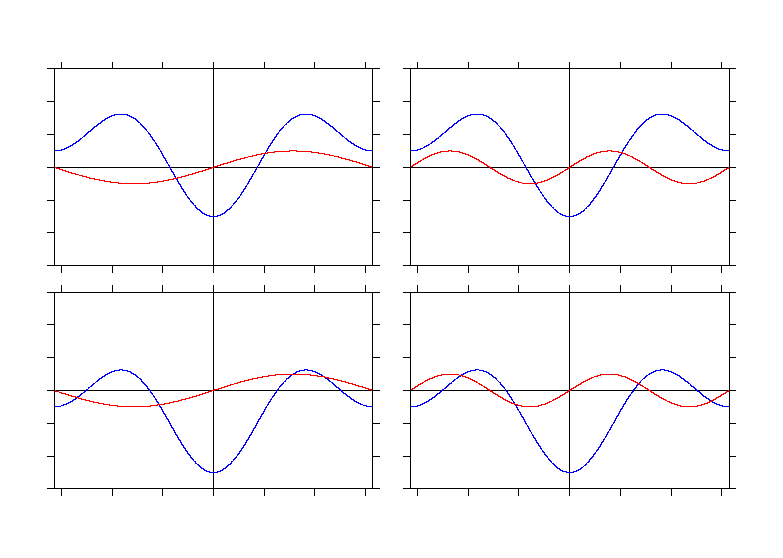
\includegraphics{Figures/Lattice.singlewire/dispersion/kdepend}}%
    \gplfronttext
  \end{picture}%
\endgroup
  
\caption{The pairings $\Delta^{11}_k$ (odd) and $\Delta^{12}_k$ (even) plotted as a function of $k$ for $\Delta^{12}_k$ imaginary. We see, that the functional behaviour is independent of $d$, and that there is a transition between interwire and intrawire dominated pairing. The intrawire pairing is increased as $d$ increases. Vice versa for the interwire pairing. Parameters: $(n_Ba_B^3)^{1/3} = 0.01$, $(n_Ba_{BF}^3)^{1/3} = 0.11$, $l_t = 0$, $\frac{m_B}{m_F} = 7/40$, $\frac{n_F}{n_B^{1/3}} = 0.215$, $v_F/c_0 = 0.33$. }  
\label{fig.pairingkdependT0dvaried}  
\end{center}    
\end{figure}

Next, we calculate the temperature dependency of the pairings. The expected behaviour can be inferred from the standard BCS-treatment, see e.g. \cite[p. 369]{PlischkeStatPhys}. From here we expect that the pairings have their maximal value for $T = 0$ and decreases monotonically until a critical temperature, $T_c$, is reached. It is however not entirely clear, what effect the presence of two pairings has on this behaviour. 

The result of the analysis for a dominant intrawire pairing is shown in figure \ref{fig.maximalpairingsTdepend_2wires}. We see, that the overall expected behaviour is observed. We observe that the intrawire pairing has a small downward kink, where the interwire pairing vanishes. The same behaviour is seen when the interwire pairing is dominant. This means, that the dominant pairing would be higher at low temperatures if the other pairing was not present: there is a trade off between the size of the individual pairings and the presence of a second pairing.

\begin{figure} 
\begin{center}  
\input{Figures/twowires/Deltas4.5/Tdepend.tex}  
\caption{Blue solid line: $\max_k[|\Delta^{12}_k|]$ as a function of temperature. Blue dashed line: asymptotic form due to Landau's theory of phase transitions, see equation \eqref{eq.DeltaasymptoteTc}. Red solid line: $\max_k[|\Delta^{11}_k|]$ as a function of temperature. Red dashed line: asymptotic form due to Landau's theory of phase transitions, see equation \eqref{eq.DeltaasymptoteTc}. Notice, that there are two critical temperatures, and that the intrawire pairing shows a downward kink, where the interwire pairing goes to zero. Parameters: $k_Fd = 0.748$, $(n_Ba_B^3)^{1/3} = 0.01$, $(n_Ba_{BF}^3)^{1/3} = 0.11$, $l_t = 0$, $\frac{m_B}{m_F} = 7/40$, $\frac{n_F}{n_B^{1/3}} = 0.215$, $v_F/c_0 = 0.33$.}  
\label{fig.maximalpairingsTdepend_2wires}  
\end{center}    
\end{figure}

The plot shows two phase transitions, one where the \textit{inter}wire pairing goes to zero and one where the \textit{intra}wire pairing goes to zero. These happen at two different critical temperatures, $T^{11}_{c}$ and $T^{12}_{c}$. Near these phase transitions, it is a general result due to Landau, that the order parameter goes as $\sqrt{1 - T/T^{ij}_c}$, see section \ref{sec.landauphasetransitions} and \cite[86-87]{PlischkeStatPhys}. The pairing potentials are linearly dependent on the mean fields, $\braket{c_{i, -k}c_{j,k}}$, which are the order parameters in the present case. Hence, close to the critical temperatures $T^{ij}_c$ we must have:
\begin{equation}
\max_k[\Delta^{ij}_k](T) = \alpha_{ij} \max_k[\Delta^{ij}_k](T = 0) \sqrt{1 - T/T^{ij}_c}. 
\label{eq.DeltaasymptoteTc}
\end{equation}
We fit these functions to the data close to the critical temperatures by adjusting $\alpha_{ij}$. This results in the dashed lines in figure \ref{fig.maximalpairingsTdepend_2wires}. We observe an excellent agreement. 

In conclusion, the presence of a second type of pairing changes the functional dependency on temperature and lowers the dominant pairing. However, the calculated temperature dependency of the pairings are entirely reliable. This is due to the increasing phase fluctuations with increasing temperature. Significant steps beyond our current formalism must be taken to come with more reliable calculations of the temperature dependency. We will not pursue this any further. For an analysis on the critical temperature of the separated wires within our current formalism the reader is referred to appendix \ref{Appendix.criticaltemperature}. 

\section{Pair wave functions} \label{sec.pairwavefunctions}
To get a physically clearer picture of the effect of the pairings we calculate the pair wave functions in real space. These are correlation functions, that describe how two fermions are correlated as a function of there respective positions. Specifically a high absolute value of $\braket{\psi_{i,F}(x')\psi_{j,F}(x)}$ for specific $x$ and $x'$ means, that the fermions have a tendency to be at those positions $x$ and $x'$. This is the reason why we refer to them as pair wave functions. However, caution should be taken, since the correlation functions are not a direct measure of probability. 

We use the Fourier decomposition $\psi_{1,F}(x) = \frac{1}{\sqrt{\mathcal{L}}} \sum_k \text{e}^{ikx} c_{1,k}$ to get an expression for the pair wave functions. For the fermions in wire 1, we get:
\begin{equation}
\braket{\psi_{1,F}(x')\psi_{1,F}(x)} = \frac{1}{\mathcal{L}} \sum_{k,q} \text{e}^{i(kx' + qx)}\braket{c_{1,k}c_{1,q}} = \frac{1}{\mathcal{L}} \sum_{k} \text{e}^{ik(x' - x)}\braket{c_{1,k}c_{1,-k}} = \frac{i}{\mathcal{L}} \sum_{k} \sin\left(k(x' - x)\right)\braket{c_{1,k}c_{1,-k}}. \nonumber 
\end{equation}
Here we first use, that we consider only states, where opposite momenta couples: $q = -k$. Then we use, that the fermionic operators anticommute, so that $c_{1,k}c_{1,-k}$ is odd in $k$. We notice, that it only depends on the difference $x' - x$. We therefore let $x \to 0$ and $x' \to x$. We then insert the mean field of equation \eqref{eq.meanfield11} for $\Delta^{12}_k$ imaginary, and get:
\begin{equation}
\braket{\psi_{1,F}(x)\psi_{1,F}(0)} = - \braket{\psi_{2,F}(x)\psi_{2,F}(0)} = \frac{i}{\mathcal{L}}\sum_k \sin(kx) \frac{\Delta^{11}_k}{2E_{F,k}}\tanh\left[\frac{ \beta E_{F,k} }{2}\right], 
\label{eq.intrawirepairwavefunction}
\end{equation}
The same calculation is carried through for the interwire pair wave function. This gives:
\begin{equation}
\braket{\psi_{1,F}(x)\psi_{2,F}(0)} = \frac{1}{\mathcal{L}}\sum_k \cos(kx) \frac{\Delta^{12}_k}{2E_{F,k}}\tanh\left[\frac{ \beta E_{F,k} }{2}\right].
\label{eq.interwirepairwavefunction}
\end{equation} 
Here we should note, that if $E^\pm_{F,k} \neq E_{F,k}$ then the above pair wave functions will be altered. From this we can infer an overall functional behaviour. Firstly, we see that $\braket{\psi_{1,F}(x)\psi_{1,F}(0)}$ and $\braket{\psi_{1,F}(x)\psi_{2,F}(0)}$ are respectively odd and even in $x$. Further, $\sin(kx)$ and $\cos(kx)$ oscillate more rapidly as a function of $k$ at higher values of $x$. Therefore, we expect the pair wave functions to decay to 0. This is also physically reasonable: fermions macroscopically far apart should not be correlated. 

A high value of $\left|\braket{\psi_{1,F}(x)\psi_{1,F}(0)}\right|$ means, that there is a tendency of two particles in the same wire to have the interparticle distance $x$. Similarly a high value of $\left|\braket{\psi_{1,F}(x)\psi_{2,F}(0)}\right|$ means, that if a fermion in wire 2 is located at $x' = 0$, there is a tendency of a second fermion to be located at the position $x$ in wire 1.  

\begin{figure} 
\begin{center}  
\input{Figures/twowires/pairwavefunctions/xdepend11.tex}  
\caption{The \textit{intra}wire pairwave function $\braket{\psi_{1,F}(x)\psi_{1,F}(0)}$ as a function of $x$ for $\Delta^{12}_k$ imaginary. We see, that the functional behaviour is independent of $d$, the pair wave function is simply decreased as $d$ decreases. Parameters: $(n_Ba_B^3)^{1/3} = 0.01$, $(n_Ba_{BF}^3)^{1/3} = 0.11$, $l_t = 0$, $\frac{m_B}{m_F} = 7/40$, $\frac{n_F}{n_B^{1/3}} = 0.215$, $v_F/c_0 = 0.33$. }  
\label{fig.2wirespairwavefunction11}  
\vspace{0.5cm}
\input{Figures/twowires/pairwavefunctions/xdepend12.tex}  
\caption{The \textit{inter}wire pairwave function $\braket{\psi_{1,F}(x)\psi_{2,F}(0)}$ as a function of $x$ for $\Delta^{12}_k$ imaginary. We see, that the functional behaviour is independent of $d$, the pair wave function is simply increased as $d$ decreases. Parameters: $(n_Ba_B^3)^{1/3} = 0.01$, $(n_Ba_{BF}^3)^{1/3} = 0.11$, $l_t = 0$, $\frac{m_B}{m_F} = 7/40$, $\frac{n_F}{n_B^{1/3}} = 0.215$, $v_F/c_0 = 0.33$. }  
\label{fig.2wirespairwavefunction12}  
\end{center}    
\end{figure}

\begin{figure}
\center
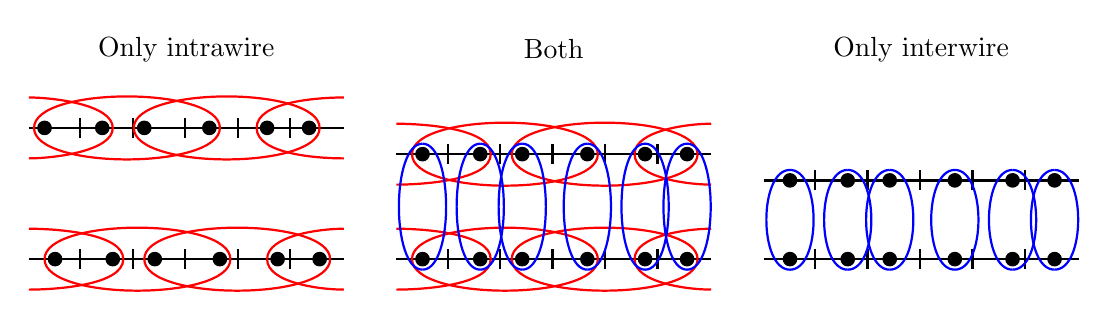
\begin{tikzpicture}[scale=2/3]
\pgfmathsetmacro{\hmove}{0}
\pgfmathsetmacro{\distance}{2.5}

\node at (3 + \hmove, 4) {Only intrawire};

\coordinate (a1) at (0.5 + \hmove, 0.14);
\coordinate (a2) at (1.6 + \hmove, 0.14);
\coordinate (a3) at (2.4 + \hmove, 0.14);
\coordinate (correlation) at (3.14, 0);

%Bottom:

\draw[-, thick]  (0 + \hmove, 0) -- (6 + \hmove, 0);
\draw[-|, thick] (0 + \hmove, 0) -- (1 + \hmove, 0);
\draw[-|, thick] (1 + \hmove, 0) -- (2 + \hmove, 0);
\draw[-|, thick] (2 + \hmove, 0) -- (3 + \hmove, 0);
\draw[-|, thick] (3 + \hmove, 0) -- (4 + \hmove, 0);
\draw[-|, thick] (4 + \hmove, 0) -- (5 + \hmove, 0);

\draw[*-, semithick] (a1); 
\draw[*-, semithick] (a1) + (correlation);
%correlation 1:
\coordinate (cor11) at (0.5 - 0.2 + \hmove, 0);
\coordinate (cor12) at (3.14 + 0.5 + 0.2 + \hmove , 0);
\draw[-, thick, red]  (cor11) to[out=90, in=90, distance=0.8cm] (cor12);
\draw[-, thick, red]  (cor11) to[out=-90, in=-90, distance=0.8cm] (cor12);

\draw[*-, semithick] (a2);
\draw[*-, semithick] (a2) + (correlation);
%correlation 2 and 4:
\coordinate (cor21) at (1.6 + 0.2 + \hmove, 0);
\coordinate (prior1) at (0 + \hmove,  0.58);
\coordinate (prior2) at (0 + \hmove, -0.58);

\coordinate (cor22) at (1.6 + 3.14 - 0.2 + \hmove , 0);
\coordinate (post1) at (6 + \hmove,  0.58);
\coordinate (post2) at (6 + \hmove, -0.58);

\draw[-, thick, red]  (cor21) to[out= 90, in=0, distance=0.5cm] (prior1);
\draw[-, thick, red]  (cor21) to[out=-90, in=0, distance=0.5cm] (prior2);

\draw[-, thick, red]  (cor22) to[out= 90, in=180, distance=0.45cm] (post1);
\draw[-, thick, red]  (cor22) to[out=-90, in=180, distance=0.45cm] (post2);

\draw[*-, semithick] (a3);
\draw[*-, semithick] (a3) + (correlation);
%correlation 3:
\coordinate (cor31) at (2.4 - 0.2 + \hmove, 0);
\coordinate (cor32) at (2.4 + 3.14 + 0.2 + \hmove, 0);
\draw[-, thick, red]  (cor31) to[out=90, in=90, distance=0.8cm] (cor32);
\draw[-, thick, red]  (cor31) to[out=-90, in=-90, distance=0.8cm] (cor32);


%Top:
\pgfmathsetmacro{\hmovetoppoints}{-0.2}
\coordinate (a1) at (0.5 + \hmove + \hmovetoppoints, 0.14 + \distance);
\coordinate (a2) at (1.6 + \hmove + \hmovetoppoints, 0.14 + \distance);
\coordinate (a3) at (2.4 + \hmove + \hmovetoppoints, 0.14 + \distance);

\draw[-, thick]  (0 + \hmove, 0 + \distance) -- (6 + \hmove, 0 + \distance);
\draw[-|, thick] (0 + \hmove, 0 + \distance) -- (1 + \hmove, 0 + \distance);
\draw[-|, thick] (1 + \hmove, 0 + \distance) -- (2 + \hmove, 0 + \distance);
\draw[-|, thick] (2 + \hmove, 0 + \distance) -- (3 + \hmove, 0 + \distance);
\draw[-|, thick] (3 + \hmove, 0 + \distance) -- (4 + \hmove, 0 + \distance);
\draw[-|, thick] (4 + \hmove, 0 + \distance) -- (5 + \hmove, 0 + \distance);

\draw[*-, semithick] (a1); 
\draw[*-, semithick] (a1) + (correlation);
%correlation 1:
\coordinate (cor11) at (0.5 - 0.2 + \hmove + \hmovetoppoints, 0 + \distance);
\coordinate (cor12) at (3.14 + 0.5 + 0.2 + \hmove + \hmovetoppoints, 0 + \distance);
\draw[-, thick, red]  (cor11) to[out=90, in=90, distance=0.8cm] (cor12);
\draw[-, thick, red]  (cor11) to[out=-90, in=-90, distance=0.8cm] (cor12);

\draw[*-, semithick] (a2);
\draw[*-, semithick] (a2) + (correlation);
%correlation 2 and 4:
\coordinate (cor21) at (1.6 + 0.2 + \hmove + \hmovetoppoints, 0 + \distance);
\coordinate (prior1) at (0 + \hmove,  0.58 + \distance);
\coordinate (prior2) at (0 + \hmove, -0.58 + \distance);

\coordinate (cor22) at (1.6 + 3.14 - 0.2 + \hmove + \hmovetoppoints , 0 + \distance);
\coordinate (post1) at (6 + \hmove,  0.58 + \distance);
\coordinate (post2) at (6 + \hmove, -0.58 + \distance);

\draw[-, thick, red]  (cor21) to[out= 90, in=0, distance=0.45cm] (prior1);
\draw[-, thick, red]  (cor21) to[out=-90, in=0, distance=0.45cm] (prior2);

\draw[-, thick, red]  (cor22) to[out= 90, in=180, distance=0.5cm] (post1);
\draw[-, thick, red]  (cor22) to[out=-90, in=180, distance=0.5cm] (post2);

\draw[*-, semithick] (a3);
\draw[*-, semithick] (a3) + (correlation);
%correlation 3:
\coordinate (cor31) at (2.4 - 0.2 + \hmove + \hmovetoppoints, 0 + \distance);
\coordinate (cor32) at (2.4 + 3.14 + 0.2 + \hmove + \hmovetoppoints, 0 + \distance);
\draw[-, thick, red]  (cor31) to[out=90, in=90, distance=0.8cm] (cor32);
\draw[-, thick, red]  (cor31) to[out=-90, in=-90, distance=0.8cm] (cor32);

%%%%%%%%%%%%%%%%%%%%%%%%%%%%%%%%
%%%%%%%%%%%%%%%%%%%%%%%%%%%%%%%%
%%%%%%%%%%%%%%%%%%%%%%%%%%%%%%%%

\pgfmathsetmacro{\hmove}{7}
\pgfmathsetmacro{\distance}{2}

\node at (3 + \hmove, 4) {Both};

\coordinate (a1) at (0.5 + \hmove, 0.14);
\coordinate (a2) at (1.6 + \hmove, 0.14);
\coordinate (a3) at (2.4 + \hmove, 0.14);
\coordinate (correlation) at (3.14, 0);

%Bottom:

\draw[-, thick]  (0 + \hmove, 0) -- (6 + \hmove, 0);
\draw[-|, thick] (0 + \hmove, 0) -- (1 + \hmove, 0);
\draw[-|, thick] (1 + \hmove, 0) -- (2 + \hmove, 0);
\draw[-|, thick] (2 + \hmove, 0) -- (3 + \hmove, 0);
\draw[-|, thick] (3 + \hmove, 0) -- (4 + \hmove, 0);
\draw[-|, thick] (4 + \hmove, 0) -- (5 + \hmove, 0);

\draw[*-, semithick] (a1); 
\draw[*-, semithick] (a1) + (correlation);
%correlation 1:
\coordinate (cor11) at (0.5 - 0.2 + \hmove, 0);
\coordinate (cor12) at (3.14 + 0.5 + 0.2 + \hmove , 0);
\draw[-, thick, red]  (cor11) to[out=90, in=90, distance=0.8cm] (cor12);
\draw[-, thick, red]  (cor11) to[out=-90, in=-90, distance=0.8cm] (cor12);

\draw[*-, semithick] (a2);
\draw[*-, semithick] (a2) + (correlation);
%correlation 2 and 4:
\coordinate (cor21) at (1.6 + 0.2 + \hmove, 0);
\coordinate (prior1) at (0 + \hmove,  0.58);
\coordinate (prior2) at (0 + \hmove, -0.58);

\coordinate (cor22) at (1.6 + 3.14 - 0.2 + \hmove , 0);
\coordinate (post1) at (6 + \hmove,  0.58);
\coordinate (post2) at (6 + \hmove, -0.58);

\draw[-, thick, red]  (cor21) to[out= 90, in=0, distance=0.5cm] (prior1);
\draw[-, thick, red]  (cor21) to[out=-90, in=0, distance=0.5cm] (prior2);

\draw[-, thick, red]  (cor22) to[out= 90, in=180, distance=0.45cm] (post1);
\draw[-, thick, red]  (cor22) to[out=-90, in=180, distance=0.45cm] (post2);

\draw[*-, semithick] (a3);
\draw[*-, semithick] (a3) + (correlation);
%correlation 3:
\coordinate (cor31) at (2.4 - 0.2 + \hmove, 0);
\coordinate (cor32) at (2.4 + 3.14 + 0.2 + \hmove, 0);
\draw[-, thick, red]  (cor31) to[out=90, in=90, distance=0.8cm] (cor32);
\draw[-, thick, red]  (cor31) to[out=-90, in=-90, distance=0.8cm] (cor32);


%Top:
\coordinate (a1) at (0.5 + \hmove, 0.14 + \distance);
\coordinate (a2) at (1.6 + \hmove, 0.14 + \distance);
\coordinate (a3) at (2.4 + \hmove, 0.14 + \distance);

\draw[-, thick]  (0 + \hmove, 0 + \distance) -- (6 + \hmove, 0 + \distance);
\draw[-|, thick] (0 + \hmove, 0 + \distance) -- (1 + \hmove, 0 + \distance);
\draw[-|, thick] (1 + \hmove, 0 + \distance) -- (2 + \hmove, 0 + \distance);
\draw[-|, thick] (2 + \hmove, 0 + \distance) -- (3 + \hmove, 0 + \distance);
\draw[-|, thick] (3 + \hmove, 0 + \distance) -- (4 + \hmove, 0 + \distance);
\draw[-|, thick] (4 + \hmove, 0 + \distance) -- (5 + \hmove, 0 + \distance);

\draw[*-, semithick] (a1); 
\draw[*-, semithick] (a1) + (correlation);
%correlation 1:
\coordinate (cor11) at (0.5 - 0.2 + \hmove, 0 + \distance);
\coordinate (cor12) at (3.14 + 0.5 + 0.2 + \hmove , 0 + \distance);
\draw[-, thick, red]  (cor11) to[out=90, in=90, distance=0.8cm] (cor12);
\draw[-, thick, red]  (cor11) to[out=-90, in=-90, distance=0.8cm] (cor12);

\draw[*-, semithick] (a2);
\draw[*-, semithick] (a2) + (correlation);
%correlation 2 and 4:
\coordinate (cor21) at (1.6 + 0.2 + \hmove, 0 + \distance);
\coordinate (prior1) at (0 + \hmove,  0.58 + \distance);
\coordinate (prior2) at (0 + \hmove, -0.58 + \distance);

\coordinate (cor22) at (1.6 + 3.14 - 0.2 + \hmove , 0 + \distance);
\coordinate (post1) at (6 + \hmove,  0.58 + \distance);
\coordinate (post2) at (6 + \hmove, -0.58 + \distance);

\draw[-, thick, red]  (cor21) to[out= 90, in=0, distance=0.5cm] (prior1);
\draw[-, thick, red]  (cor21) to[out=-90, in=0, distance=0.5cm] (prior2);

\draw[-, thick, red]  (cor22) to[out= 90, in=180, distance=0.45cm] (post1);
\draw[-, thick, red]  (cor22) to[out=-90, in=180, distance=0.45cm] (post2);

\draw[*-, semithick] (a3);
\draw[*-, semithick] (a3) + (correlation);
%correlation 3:
\coordinate (cor31) at (2.4 - 0.2 + \hmove, 0 + \distance);
\coordinate (cor32) at (2.4 + 3.14 + 0.2 + \hmove, 0 + \distance);
\draw[-, thick, red]  (cor31) to[out=90, in=90, distance=0.8cm] (cor32);
\draw[-, thick, red]  (cor31) to[out=-90, in=-90, distance=0.8cm] (cor32);

%interwire correlations:

%correlation 1 and 4:
\coordinate (cor11) at (0.5 + \hmove, 0 - 0.2);
\coordinate (cor12) at (0.5 + \hmove, 0 + 0.2 + \distance);
\coordinate (cor13) at (0.5 + 3.14 + \hmove, 0 + 0.2 + \distance);
\draw[-, thick, blue]  (cor11) to[out=0, in=0, distance=0.6cm] (cor12);
\draw[-, thick, blue]  (cor11) to[out=180, in=180, distance=0.6cm] (cor12);

\draw[-, thick, blue]  (cor11) + (correlation) to[out=0, in=0, distance=0.6cm] (cor13);
\draw[-, thick, blue]  (cor11) + (correlation) to[out=180, in=180, distance=0.6cm] (cor13);

%correlation 2:
\coordinate (cor21) at (1.6 + \hmove, 0 - 0.2);
\coordinate (cor22) at (1.6 + \hmove, 0 + 0.2 + \distance);
\draw[-, thick, blue]  (cor21) to[out=0, in=0, distance=0.6cm] (cor22);
\draw[-, thick, blue]  (cor21) to[out=180, in=180, distance=0.6cm] (cor22);

%correlation 3 and 6:
\coordinate (cor31) at (2.4 + \hmove, 0 - 0.2);
\coordinate (cor32) at (2.4 + \hmove, 0 + 0.2 + \distance);
\coordinate (cor33) at (2.4 + 3.14 + \hmove, 0 + 0.2 + \distance);
\draw[-, thick, blue]  (cor31) to[out=0, in=0, distance=0.6cm] (cor32);
\draw[-, thick, blue]  (cor31) to[out=180, in=180, distance=0.6cm] (cor32);

\draw[-, thick, blue]  (cor31) + (correlation) to[out=0, in=0, distance=0.6cm] (cor33);
\draw[-, thick, blue]  (cor31) + (correlation) to[out=180, in=180, distance=0.6cm] (cor33);

%correlation 5:
\coordinate (cor51) at (1.6 + 3.14 + \hmove, 0 - 0.2);
\coordinate (cor52) at (1.6 + 3.14 + \hmove, 0 + 0.2 + \distance);
\draw[-, thick, blue]  (cor51) to[out=0, in=0, distance=0.6cm] (cor52);
\draw[-, thick, blue]  (cor51) to[out=180, in=180, distance=0.6cm] (cor52);

%%%%%%%%%%%%%%%%%%%%%%%%%%%%%%%%
%%%%%%%%%%%%%%%%%%%%%%%%%%%%%%%%
%%%%%%%%%%%%%%%%%%%%%%%%%%%%%%%%

\pgfmathsetmacro{\hmove}{14}
\pgfmathsetmacro{\distance}{1.5}

\node at (3 + \hmove, 4) {Only interwire};

\coordinate (a1) at (0.5 + \hmove, 0.14);
\coordinate (a2) at (1.6 + \hmove, 0.14);
\coordinate (a3) at (2.4 + \hmove, 0.14);
\coordinate (correlation) at (3.14, 0);

%Bottom:

\draw[-, thick]  (0 + \hmove, 0) -- (6 + \hmove, 0);
\draw[-|, thick] (0 + \hmove, 0) -- (1 + \hmove, 0);
\draw[-|, thick] (1 + \hmove, 0) -- (2 + \hmove, 0);
\draw[-|, thick] (2 + \hmove, 0) -- (3 + \hmove, 0);
\draw[-|, thick] (3 + \hmove, 0) -- (4 + \hmove, 0);
\draw[-|, thick] (4 + \hmove, 0) -- (5 + \hmove, 0);

\draw[*-, semithick] (a1); 
\draw[*-, semithick] (a1) + (correlation);
\draw[*-, semithick] (a2);
\draw[*-, semithick] (a2) + (correlation);
\draw[*-, semithick] (a3);
\draw[*-, semithick] (a3) + (correlation);


%Top:
\coordinate (a1) at (0.5 + \hmove, 0.14 + \distance);
\coordinate (a2) at (1.6 + \hmove, 0.14 + \distance);
\coordinate (a3) at (2.4 + \hmove, 0.14 + \distance);

\draw[-, thick]  (0 + \hmove, 0 + \distance) -- (6 + \hmove, 0 + \distance);
\draw[-|, thick] (0 + \hmove, 0 + \distance) -- (1 + \hmove, 0 + \distance);
\draw[-|, thick] (1 + \hmove, 0 + \distance) -- (2 + \hmove, 0 + \distance);
\draw[-|, thick] (2 + \hmove, 0 + \distance) -- (3 + \hmove, 0 + \distance);
\draw[-|, thick] (3 + \hmove, 0 + \distance) -- (4 + \hmove, 0 + \distance);
\draw[-|, thick] (4 + \hmove, 0 + \distance) -- (5 + \hmove, 0 + \distance);

\draw[*-, semithick] (a1); 
\draw[*-, semithick] (a1) + (correlation);
\draw[*-, semithick] (a2);
\draw[*-, semithick] (a2) + (correlation);
\draw[*-, semithick] (a3);
\draw[*-, semithick] (a3) + (correlation);

%interwire correlations:

%correlation 1 and 4:
\coordinate (cor11) at (0.5 + \hmove, 0 - 0.2);
\coordinate (cor12) at (0.5 + \hmove, 0 + 0.2 + \distance);
\coordinate (cor13) at (0.5 + 3.14 + \hmove, 0 + 0.2 + \distance);
\draw[-, thick, blue]  (cor11) to[out=0, in=0, distance=0.6cm] (cor12);
\draw[-, thick, blue]  (cor11) to[out=180, in=180, distance=0.6cm] (cor12);

\draw[-, thick, blue]  (cor11) + (correlation) to[out=0, in=0, distance=0.6cm] (cor13);
\draw[-, thick, blue]  (cor11) + (correlation) to[out=180, in=180, distance=0.6cm] (cor13);

%correlation 2:
\coordinate (cor21) at (1.6 + \hmove, 0 - 0.2);
\coordinate (cor22) at (1.6 + \hmove, 0 + 0.2 + \distance);
\draw[-, thick, blue]  (cor21) to[out=0, in=0, distance=0.6cm] (cor22);
\draw[-, thick, blue]  (cor21) to[out=180, in=180, distance=0.6cm] (cor22);

%correlation 3 and 6:
\coordinate (cor31) at (2.4 + \hmove, 0 - 0.2);
\coordinate (cor32) at (2.4 + \hmove, 0 + 0.2 + \distance);
\coordinate (cor33) at (2.4 + 3.14 + \hmove, 0 + 0.2 + \distance);
\draw[-, thick, blue]  (cor31) to[out=0, in=0, distance=0.6cm] (cor32);
\draw[-, thick, blue]  (cor31) to[out=180, in=180, distance=0.6cm] (cor32);

\draw[-, thick, blue]  (cor31) + (correlation) to[out=0, in=0, distance=0.6cm] (cor33);
\draw[-, thick, blue]  (cor31) + (correlation) to[out=180, in=180, distance=0.6cm] (cor33);

%correlation 5:
\coordinate (cor51) at (1.6 + 3.14 + \hmove, 0 - 0.2);
\coordinate (cor52) at (1.6 + 3.14 + \hmove, 0 + 0.2 + \distance);
\draw[-, thick, blue]  (cor51) to[out=0, in=0, distance=0.6cm] (cor52);
\draw[-, thick, blue]  (cor51) to[out=180, in=180, distance=0.6cm] (cor52);

\end{tikzpicture}
\caption{Spatial distribution of the fermions along the wires. Intrawire and interwire correlations are shown in red and blue respectively. Left: large interwire distances. The fermions correlate internally in each wire only. Middle: intermediate interwire distances. The fermions correlate both internally and across the wires. Right: small interwire distances. The fermions only correlate across the wires.}
\label{fig.2wirespositioncorrelations}
\end{figure}

By using the pairings found in the above analysis we can readily calculate the pair wave functions numerically. The result is shown in figures \ref{fig.2wirespairwavefunction11} and \ref{fig.2wirespairwavefunction12}. They have the following physical interpretation. The \textit{intra}wire pair wave function: fermions correlate over several interparticle distances. The correlation is decreased when we decrease the interwire distance, $d$. The \textit{inter}wire pair wave function: there is a tendency of a fermion in wire 1 to be facing a fermion in wire 2. This correlation is increased as $d$ decreases. 

In figure \ref{fig.2wirespositioncorrelations} we depict these correlations in a pictorial manner. From here it is also evident, that the pairing tend to order the system. In turn the entropy is lowered. 

\section{Occupancy and energy dispersion}
\label{subsec.relevantmomenta.effectiveinteraction}
In this subsection we will briefly study the energy dispersion and the mean occupancy of the $k$'th state. This will in more detail explain, why it is momenta around the Fermi momentum ($k \approx k_F$), that are relevant to understand the influence of the pairing.  

In figures \ref{fig.EnergyDispersion} and \ref{fig.Occupancy} we have plotted the energy dispersion $E_{F,k}$ and occupancy $\braket{c_{1,k}^\dagger c_{1,k}}$ for $T = 0$. This is done for several values of the interwire distance, $d$. Notice that for $T = 0$, the occupancy from equation \eqref{eq.meanoccupancy} shows, that $\braket{c_{1,k}^\dagger c_{1,k}} = \frac{1}{2}\left(1 -  \frac{\varepsilon_k}{E_{F,k}}\right)$. 

\begin{figure} 
\begin{center}  
\input{Figures/twowires/OccupancyT0/energyplot.tex}  
\caption{The energy dispersion is plotted for $T = 0$. Coloured lines: differing values of the relative interparticle distance $n_F / n_B^{1/3}$, superfluid phase. Black line: free gas (normal phase) energy dispersion. The energy is even in $k$, so the graphs are just mirrored for $k < 0$. Parameters: $(n_Ba_B^3)^{1/3} = 0.01$, $(n_Ba_{BF}^3)^{1/3} = 0.11$, $l_t = 0$, $\frac{m_B}{m_F} = 7/40$, $\frac{n_F}{n_B^{1/3}} = 0.215$, $v_F/c_0 = 0.33$. }  
\label{fig.EnergyDispersion}  
\end{center}    
\end{figure}

The energy dispersions are qualitatively similar to the free gas shown in black. The main effect of the pairings are to round off the dispersion at $k \approx k_F$. Further, the value in $k = 0$ is increasingly shifted, with increasin interwire pairing, $\Delta^{12}_k$. This also means, that the occupancy for low $k$-states are lowered, when the interwire pairing increases. This is especially evident from the red curve in figure \ref{fig.Occupancy}. The plots makes it clear, that the relevant momenta for the pairing is around $k = k_F$. 

In our numerical analysis we have noticed, that the chemical potential is shifted \textit{down} for dominant \textit{intra}wire $p$-wave pairing and shifted \textit{up} for \textit{inter}wire $s$-wave pairing. The current analysis illuminates, why this is so. In the intrawire case is most easily understood. The attractive interaction between the wires lowers the energy required to put in an additional fermion, $E$. In turn the chemical potential $\mu = \partial E / \partial N$ is lowered. Superficially this is also true for the \textit{inter}wire interactions. However, here there is the additional effect, that the low-lying $k$-states are partially depleted. Since the chemical potential is the energy at which half the states are occupied, and since som low-lying states are gone, the chemical potential must increase. 

\begin{figure} 
\begin{center}  
\input{Figures/twowires/OccupancyT0/Occupancyplot.tex}  
\caption{The number of fermions with momentum $k$, $\braket{c_k^\dagger c_k}$, is plotted for $T = 0$. $\braket{c_k^\dagger c_k} = |v_{F,k}|^2 = \frac{1}{2}\left(1 - \frac{\epsilon_k}{E_{F,k}}\right)$. Coloured lines: differing values of the relative interparticle distance $n_F / n_B^{1/3}$, superfluid phase. Black line: Fermi-Dirac distribution for the free gas (normal phase). Other parameters: Parameters: $(n_Ba_B^3)^{1/3} = 0.01$, $(n_Ba_{BF}^3)^{1/3} = 0.11$, $l_t = 0$, $\frac{m_B}{m_F} = 7/40$, $\frac{n_F}{n_B^{1/3}} = 0.215$, $v_F/c_0 = 0.33$. }  
\label{fig.Occupancy}  
\end{center}    
\end{figure}

In connection with the neglection of retardation effects we already used, that the typical speed of the fermions is the Fermi speed $v_F = k_F/m_F$. The present subsection therefore shows, that this assumption is selfconsistent. This also means, that when we wish to characterize the interactions, we can investigate the effective interactions, $W^{ij}_{\text{ind}}(k, k')$, at the Fermi momentum. Hence, we can set $k = k' = k_F$. We will use this in the following section.


\section{Control of transition through the coherence length}
\label{sec.2wires_crossover_control_coherence_length}
In this section we will investigate how we can control the transition from intrawire to interwire pairing through the coherence length, $\xi$, of the Bose-Einstein condensate. We further investigate the effective interactions at the Fermi momentum, $W^{ij}_{\text{ind}}(k_F, k_F)$, as a function of the coherence length. 

The range of the induced interaction is the condensate coherence length:
\begin{equation}
k_F\frac{\xi}{\sqrt{2}} = \frac{\sqrt{\pi}}{4}\frac{1}{\sqrt{(n_Ba_B^3)^{1/3}}}\frac{n_F}{n_B^{1/3}}.
\label{eq.RangefunctionofrBBnB}
\end{equation}
We would like to explore the possibility of controlling the transition through the coherence length. This is of experimental relevance. Adjusting the spatial distance, $d$, between the wires may be rather difficult in an experimental setup. If we can control an effective distance between the wires by adjusting the coherence length, this then might be a more realisable approach. We have the following intuitive idea of the feasibility of this approach. For a very short coherence length the induced interaction cannot reach across the distance $d$ between the wires. However, there is always a neighbour close by internally in the wire. Hence, we expect that for $\xi \to 0$ the system is in the intrawire pairing only regime. Opposite, for very long coherence lengths the distance between the wires becomes insignificant. Further, since the interwire induced interaction is enhanced by a factor of 2 relative to the intrawire one, we expect that for $\xi \to \infty$ the system enters the interwire pairing only regime. 

The previous section suggests, that we should investigate the effective interactions at the Fermi momentum. We will use the relative particle distance $\frac{n_F}{n_B^{1/3}}$ to vary the coherence length. Hence, we plot $W^{ij}_{\text{ind}}(k_F,k_F)$ as a function of this parameter. This is shown in figure \ref{fig.EffectiveInteraction.nBdepend} for $k_Fd = 0.7$. The overall functional behaviour we understand as follows. When the density of the boson gas increases, the gas becomes increasingly rigid and the fermions have a harder time creating ripples in the gas. Therefore, the effective interactions goes down. The \textit{inter}wire interaction decreases faster, because the interaction has to reach across the interwire distance, $d$. For high values of $\frac{n_F}{n_B^{1/3}}$ on the other hand, the boson gas is depleted, $n_B$ decreases, and there are simply fewer bosons around for the fermions to interact with. Again, the effective interaction goes down. This is in complete accordance with what is seen in an equivalent 2D-3D system studied in the article \cite{BruunZhigangTopSuperfluid}. Further, we notice that in this limit the \textit{inter}wire interaction goes asymptotically to the \textit{intra}wire one. This is because in this limit, the interwire distance becomes insignificant relative to the coherence length, $\xi$. 

\begin{figure} 
\begin{center}  
% GNUPLOT: LaTeX picture with Postscript
\begingroup
  \makeatletter
  \providecommand\color[2][]{%
    \GenericError{(gnuplot) \space\space\space\@spaces}{%
      Package color not loaded in conjunction with
      terminal option `colourtext'%
    }{See the gnuplot documentation for explanation.%
    }{Either use 'blacktext' in gnuplot or load the package
      color.sty in LaTeX.}%
    \renewcommand\color[2][]{}%
  }%
  \providecommand\includegraphics[2][]{%
    \GenericError{(gnuplot) \space\space\space\@spaces}{%
      Package graphicx or graphics not loaded%
    }{See the gnuplot documentation for explanation.%
    }{The gnuplot epslatex terminal needs graphicx.sty or graphics.sty.}%
    \renewcommand\includegraphics[2][]{}%
  }%
  \providecommand\rotatebox[2]{#2}%
  \@ifundefined{ifGPcolor}{%
    \newif\ifGPcolor
    \GPcolortrue
  }{}%
  \@ifundefined{ifGPblacktext}{%
    \newif\ifGPblacktext
    \GPblacktexttrue
  }{}%
  % define a \g@addto@macro without @ in the name:
  \let\gplgaddtomacro\g@addto@macro
  % define empty templates for all commands taking text:
  \gdef\gplbacktext{}%
  \gdef\gplfronttext{}%
  \makeatother
  \ifGPblacktext
    % no textcolor at all
    \def\colorrgb#1{}%
    \def\colorgray#1{}%
  \else
    % gray or color?
    \ifGPcolor
      \def\colorrgb#1{\color[rgb]{#1}}%
      \def\colorgray#1{\color[gray]{#1}}%
      \expandafter\def\csname LTw\endcsname{\color{white}}%
      \expandafter\def\csname LTb\endcsname{\color{black}}%
      \expandafter\def\csname LTa\endcsname{\color{black}}%
      \expandafter\def\csname LT0\endcsname{\color[rgb]{1,0,0}}%
      \expandafter\def\csname LT1\endcsname{\color[rgb]{0,1,0}}%
      \expandafter\def\csname LT2\endcsname{\color[rgb]{0,0,1}}%
      \expandafter\def\csname LT3\endcsname{\color[rgb]{1,0,1}}%
      \expandafter\def\csname LT4\endcsname{\color[rgb]{0,1,1}}%
      \expandafter\def\csname LT5\endcsname{\color[rgb]{1,1,0}}%
      \expandafter\def\csname LT6\endcsname{\color[rgb]{0,0,0}}%
      \expandafter\def\csname LT7\endcsname{\color[rgb]{1,0.3,0}}%
      \expandafter\def\csname LT8\endcsname{\color[rgb]{0.5,0.5,0.5}}%
    \else
      % gray
      \def\colorrgb#1{\color{black}}%
      \def\colorgray#1{\color[gray]{#1}}%
      \expandafter\def\csname LTw\endcsname{\color{white}}%
      \expandafter\def\csname LTb\endcsname{\color{black}}%
      \expandafter\def\csname LTa\endcsname{\color{black}}%
      \expandafter\def\csname LT0\endcsname{\color{black}}%
      \expandafter\def\csname LT1\endcsname{\color{black}}%
      \expandafter\def\csname LT2\endcsname{\color{black}}%
      \expandafter\def\csname LT3\endcsname{\color{black}}%
      \expandafter\def\csname LT4\endcsname{\color{black}}%
      \expandafter\def\csname LT5\endcsname{\color{black}}%
      \expandafter\def\csname LT6\endcsname{\color{black}}%
      \expandafter\def\csname LT7\endcsname{\color{black}}%
      \expandafter\def\csname LT8\endcsname{\color{black}}%
    \fi
  \fi
    \setlength{\unitlength}{0.0500bp}%
    \ifx\gptboxheight\undefined%
      \newlength{\gptboxheight}%
      \newlength{\gptboxwidth}%
      \newsavebox{\gptboxtext}%
    \fi%
    \setlength{\fboxrule}{0.5pt}%
    \setlength{\fboxsep}{1pt}%
\begin{picture}(7200.00,5040.00)%
    \gplgaddtomacro\gplbacktext{%
      \csname LTb\endcsname%
      \put(682,1188){\makebox(0,0)[r]{\strut{}$-4$}}%
      \csname LTb\endcsname%
      \put(682,2030){\makebox(0,0)[r]{\strut{}$-2$}}%
      \csname LTb\endcsname%
      \put(682,2872){\makebox(0,0)[r]{\strut{}$0$}}%
      \csname LTb\endcsname%
      \put(682,3713){\makebox(0,0)[r]{\strut{}$2$}}%
      \csname LTb\endcsname%
      \put(682,4555){\makebox(0,0)[r]{\strut{}$4$}}%
      \csname LTb\endcsname%
      \put(877,484){\makebox(0,0){\strut{}$-10$}}%
      \csname LTb\endcsname%
      \put(2343,484){\makebox(0,0){\strut{}$-5$}}%
      \csname LTb\endcsname%
      \put(3809,484){\makebox(0,0){\strut{}$0$}}%
      \csname LTb\endcsname%
      \put(5274,484){\makebox(0,0){\strut{}$5$}}%
      \csname LTb\endcsname%
      \put(6740,484){\makebox(0,0){\strut{}$10$}}%
    }%
    \gplgaddtomacro\gplfronttext{%
      \csname LTb\endcsname%
      \put(176,2871){\rotatebox{-270}{\makebox(0,0){\strut{}$2m_F/k_F W_{	ext{ind}}(k, k_F)$}}}%
      \put(3808,154){\makebox(0,0){\strut{}$k / k_F$}}%
      \csname LTb\endcsname%
      \put(4565,4803){\makebox(0,0)[l]{\strut{}$k_Fd = 0.720$}}%
      \csname LTb\endcsname%
      \put(4565,4583){\makebox(0,0)[l]{\strut{}$k_Fd = 0.735$}}%
      \csname LTb\endcsname%
      \put(4565,4363){\makebox(0,0)[l]{\strut{}$k_Fd = 0.750$}}%
      \csname LTb\endcsname%
      \put(4565,4143){\makebox(0,0)[l]{\strut{}$k_Fd = 0.765$}}%
      \csname LTb\endcsname%
      \put(4565,3923){\makebox(0,0)[l]{\strut{}$k_Fd = 0.775$}}%
    }%
    \gplbacktext
    \put(0,0){\includegraphics{InducedInteraction}}%
    \gplfronttext
  \end{picture}%
\endgroup
  
\caption{Solid lines: The effective interactions at the Fermi surface, $W^{ij}_{\text{ind}}(k_F,k_F)$, as a function of relative particle distance $n_F/n_B^{1/3}$. Red line: intrawire effective interaction, $W^{11}_{\text{ind}}(k_F,k_F)$. Blue line: interwire effective interaction, $W^{12}_{\text{ind}}(k_F,k_F)$. Dashed line: indicates where the retardation effects are expected to kick in; the line is made by requiring $v_F/c_0 < 1$. Notice that the effective interactions have an extremal value. Parameters: $k_Fd = 0.7$, $(n_Ba_B^3)^{1/3} = 0.01, (n_Ba_{BF}^3)^{1/3} = 0.1, \frac{m_B}{m_F} = 7/40$.}  
\label{fig.EffectiveInteraction.nBdepend}  
\end{center}    
\end{figure}

We notice, that the \textit{inter}wire interaction becomes dominant around $\frac{n_F}{n_B^{1/3}} = 0.1$. This suggests, that there will be a $p$- to $s$-wave phase transition around this value. Computing whether the intrawire interaction, $W^{11}_{\text{ind}}(k_F,k_F)$, or the interwire interaction, $W^{12}_{\text{ind}}(k_F,k_F)$, is dominant results in the dot-dashed curve in figure \ref{fig.twowirescrossovernBdepend}. 

We now calculate this phase diagram in $d$ and $n_F/n_B^{1/3}$ rigorously. A direct and precise measure for the transition is the previously mentioned critical distance $d_c$. In practice this is found in the following way. First we calculate the free energy $F(\Delta^{11}_k) = E_0(\Delta^{11}_k) + 2 \mu (\Delta^{11}_k) N_F$ in the case, that there is only intrawire pairing, $\Delta^{11}_k$ present. This is independent of $d$ as described by the dashed curve in figure \ref{fig.2wiresE0ddepend}. Then we calculate the same, when only interwire pairing is present. For a constant $n_F/n_B^{1/3}$, we then iteratively find the value of $d = d_c$, where the free energies match: $F(\Delta^{12}_k, d_c) = F(\Delta^{11}_k)$. We then decrease $n_F/n_B^{1/3}$ by a small amount and repeat the process. The outcome of the analysis is shown as the black solid curve in figure \ref{fig.twowirescrossovernBdepend}. We notice, that $d_c$ exhibits a maximal value, and that it approaches a constant for large values of $n_F/n_B^{1/3}$. The dashed vertical line indicates where $v_F = c_0$. To the right of this line retardation effects are expected to kick in. 

The area with white background indicates the \textit{intra}wire pairing only regime. The grey area is correspondingly \textit{inter}wire pairing only. We can understand this result in the following way. First, consider a constant value of the relative particle distance, e.g. $n_F/n_B^{1/3} = 0.2$. When we decrease the interwire distance from say $k_Fd = 1$ we move along the dashed vertical grid line at $n_F/n_B^{1/3} = 0.2$. The system experiences the transition, when we cross the solid black line. This is as described in section \ref{sec.2wiresCrossover_energy}. Second, consider a constant value of the interwire distance, e.g. $k_Fd = 0.6$. When we increase $n_F/n_B^{1/3}$ we follow the horisontal grid line and the system again experiences the transition, when it crosses the solid black line. 

\begin{figure} 
\begin{center}  
\input{Figures/twowires/Deltas3.1.3/nBdepend.tex}  
\caption{Solid line: the critical distance $d_c$ plotted as a function of the relative particle distance $n_F/n_B^{1/3}$. White background: intrawire pairing only regime. Grey background: interwire pairing only regime. Dash-dotted line: the critical distance according to the competition of intra- and interwire interactions for $k_Fx_0 = 1/\sqrt{3}$. See equation \eqref{eq.2wires.Vequal}. When we cross the solid line the system experiences the phase transition studied in section \ref{sec.2wiresCrossover_energy}. Dashed vertical line: $v_F = c_0$. Retardation effects are expected to kick in to the right hereof. Parameters: $(n_Ba_B^3)^{1/3} = 0.01$, $(n_Ba_{BF}^3)^{1/3} = 0.11$, $l_t = 0$, $\frac{m_B}{m_F} = 7/40$. }  
\label{fig.twowirescrossovernBdepend}  
\end{center}    
\end{figure}

In this way we explicitly see, that instead of actually moving the wires we can control the transition by adjusting $n_F/n_B^{1/3}$ and in turn the coherence length; see equation \eqref{eq.RangefunctionofrBBnB}. We notice, that the simple analysis based on the effective interactions at the Fermi momentum and the more elaborate but direct calculation of the critical distance $d_c$ are qualitatively similar. However, we notice that the dip in $d_c$ for high values of $n_F/n_B^{1/3}$ is more significant, than the simple analysis suggests. This emphasizes the fact, that although a lot of physical intuition can be build on the form and behaviour of the effective interactions, we have to be careful when used to argue for the response of the system.
 

\part{Kitaev chain and winding numbers larger than 1}
\fancyhead[LE,RO]{\thepage}
In part II, we analysed the properties of two wires in a 3D BEC. We saw that when the wires were far apart, they could realise the Kitaev model with non-trivial winding numbers $w = \pm 1$. In this third part we will show that by making the boson gas one-dimensional and trapping the fermions in an optical lattice and shaking it, we can realise a Kitaev model with topological winding numbers larger than 1. In turn several edge states at the ends of the lattice emerge. It is rare to find realistic proposals like this for realising such systems. The setup is shown in the figure below. 

\vspace{2.5cm}

\begin{figure}[H]
\center
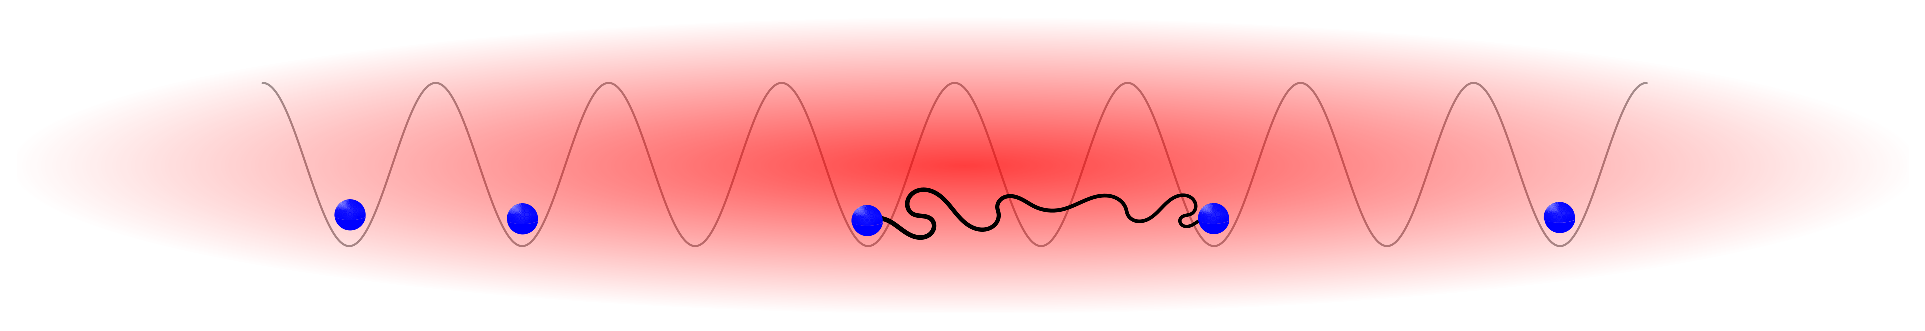
\includegraphics[width=1\columnwidth]{gasandlattice.eps}
\\ Lattice of fermions in 1D Bose gas. In blue: fermions. In red: boson gas. In grey: optical lattice. Black wiggly line: induced interaction between the fermions mediated by the bosons.   
\end{figure}

\newpage
% Chapter 7

\chapter{Topology and symmetries} % Main chapter title

\label{Chapter7} % For referencing the chapter elsewhere, use \ref{Chapter7} 

\lhead{Part II. \emph{One wire}}
\chead{Chapter 7. \emph{Topology \& symmetries}} % This is for the header on each page - perhaps a shortened title

%----------------------------------------------------------------------------------------
In this chapter we will define the socalled time reversal and particle-hole transformations. This we will use to come with a topological characterization of the now developed Kitaev model system. It entails defining a topological index $\nu$, that describes whether the system is in a topological or trivial phase. Finally, we will see what physical consequences the phases have by discussing the bulk-edge correspondence principle and edge states. The treatment is heavily based on the articles \cite{Ludwig.Topology, Chiu.Topology, Alicea}. 

\section{The time reversal and particle-hole transformations and symmetries}
\label{sec.SymmetriesTRandPH}
In this section we define the time reversal and particle-hole transformations. Let us remind ourselves of the form of the noninteracting Hamiltonian obtained after the mean field approximation of chapter \ref{Chapter4}: 
\begin{equation}
H_{FF} = -\sum_k \Delta_k \braket {c^\dagger_k c^\dagger_{-k}} + \frac{1}{2}\sum_{k} \begin{bmatrix} c^\dagger_k & c_{-k} \end{bmatrix} \begin{bmatrix} \varepsilon_k & \Delta_k \\ \Delta^*_k & -\varepsilon_k \end{bmatrix} \begin{bmatrix} c_k \\ c^\dagger_{-k} \end{bmatrix}. \nonumber 
\end{equation}

It is clear, that the Hamiltonian is translationally invariant. Explicitly, the (unitary) translation operator is defined through: $\tau(x_0)\psi_F(x)\tau^\dagger (x_0) = \psi_F(x+x_0)$. In momentum space, we hereby get $\tau(x_0) c_k \tau^\dagger(x_0) = \text{e}^{ikx_0}c_k$, as one might expect. Hence, terms like $c^\dagger_k c_k, c_k c^\dagger_k, c^\dagger_kc^\dagger_{-k}$ and $c_{-k}c_k$ are invariant under the translation. This means, that $H_{FF}$ is invariant as well. Because of the translational invariance, we \textit{inforce} that the time reversal and particle-hole transformations do not mix states with different positions. Specifically:
\begin{align}
T \begin{bmatrix} \psi_F(x) \\ \psi^\dagger_F(x) \end{bmatrix} T^{-1} &= U^\dagger_T \begin{bmatrix} \psi_F(x) \\ \psi^\dagger_F(x) \end{bmatrix}, \hspace{0.5cm} TiT^{-1} = -i, \nonumber \\
C \begin{bmatrix} \psi_F(x) \\ \psi^\dagger_F(x) \end{bmatrix} C^{-1} &= (U^*_C)^\dagger \begin{bmatrix} \psi^\dagger_F(x) \\ \psi_F(x) \end{bmatrix}, \hspace{0.5cm} CiC^{-1} = i.  
\label{eq.TRandPH.realspace}
\end{align}
Here $T$ and $C$ is the time reversal and particle-hole transformation respectively. $U_T$ and $U_C$ are $2\times 2$ matrices. Inforcing that transformed operators are fermionic as well, means that the matrices have to be unitary. The operation on $i$ specifies, that $T$ is antiunitary and $C$ is unitary. In momentum space this definition leads to:
\begin{align}
T \begin{bmatrix} c_k \\ c^\dagger_{-k} \end{bmatrix} T^{-1} &= U^\dagger_T \begin{bmatrix} c_{-k} \\ c^\dagger_{k} \end{bmatrix}, \nonumber \\
C \begin{bmatrix} c_k \\ c^\dagger_{-k} \end{bmatrix} C^{-1} &= (U^*_C)^\dagger \begin{bmatrix} c^\dagger_{-k} \\ c_{k} \end{bmatrix}. 
\label{eq.TRandPH.momentumspace}
\end{align}
By inspecting the transformations $TH_{FF}T^{-1}$ and $CH_{FF}C^{-1}$, we get the following symmetry requirements:
\begin{align}
TH_{FF}T^{-1} = H_{FF} \Leftrightarrow U_T\mathcal{H}^*_{FF,-k} U^\dagger_T = + \mathcal{H}_{FF,+k}, \nonumber \\
CH_{FF}T^{-1} = H_{FF} \Leftrightarrow U_C\mathcal{H}^*_{FF,-k} U^\dagger_C = - \mathcal{H}_{FF,+k}. 
\label{eq.Symmetryrequirements}
\end{align}
This means, that we can think of the second quantization transformations $T$ and $C$ in terms of first quantization antiunitary transformations $\mathcal{T} = U_TK, \mathcal{C} = U_CK$, where $K$ is the complex conjugation operator. This is a general property of these transformation, not restricted to our specific system. See e.g. the articles \cite{Ludwig.Topology, Chiu.Topology}. The Hamiltonian at hand is a socalled Bogoliubov-de Gennes (BdG) Hamiltonian. These BdG Hamiltonians in general has a particle-hole symmetry. The reason is, that there is a redundancy in the matrix structure of the Hamiltonian. Explicitly, the structure contains a $2\times 2$ matrix, even though there is only one energy solution. Another way of putting this, is that the two Nambu spinors on each side of the kernel $\mathcal{H}_{FF,k}$ are not independent. We can transform one into the other by going to $-k$ and flipping the entries. The redundancy is here especially evident, since we can simply choose $C$ to have no effect on the Nambu spinor:
\begin{equation}
C \begin{bmatrix} c_k \\ c^\dagger_{-k} \end{bmatrix} C^{-1} =  \sigma_1 \begin{bmatrix} c^\dagger_{-k} \\ c_{k} \end{bmatrix} = \begin{bmatrix} c_k \\ c^\dagger_{-k} \end{bmatrix}, 
\end{equation}
with $\sigma_1$ the first Pauli matrix. This of course means, that $H_{FF}$ is invariant under $C$. Since, it stems from a redundancy in the \textit{structure} of the Hamiltonian, it is often referred to as a particle-hole \textit{constraint} of BdG systems rather than a symmetry. This also means, that for the system to be consistent, we need $\sigma_1\mathcal{H}^*_{FF,+k} \sigma_1 = - \mathcal{H}_{FF,-k}$, which can also explicitly be checked. 

The time reversal case is somewhat trickier. Firstly, in general the pairing $\Delta_k$ is complex. However, as seen in the previous chapters we can explicitly find a real solution. This is also evident mathematically. For this purpose we let $\Delta_k \to \text{e}^{i\phi}\Delta_k$, with $\phi$ the phase of the pairing, and now $\Delta_k$ real. We then perform a gauge transformation in the $c_k$ operators according to: $c_k \to \text{e}^{-i\phi/2} c_k$. Since $\Delta_k$ depends linearly on $\braket{c_kc_{-k}}$ the resulting transformation of the pairing is:
\begin{equation}
\text{e}^{i\phi}\Delta_k \to \text{e}^{i\phi}\Delta_k\text{e}^{-i\phi} = \Delta_k. \nonumber
\end{equation}
With this the kernel $\mathcal{H}_{FF,k}$ is real, and with $U_T = i\sigma_3$ we get a time reversal symmetry in accordance with equation \ref{eq.Symmetryrequirements}. Explicitly:
\begin{equation}
U_T\mathcal{H}^*_{FF,-k}U^\dagger_T = \sigma_3\mathcal{H}^*_{FF,-k}\sigma_3 = \begin{bmatrix} 1 & 0 \\ 0 & -1 \end{bmatrix}\begin{bmatrix} \varepsilon_k & -\Delta_k \\ -\Delta_k & -\varepsilon_k \end{bmatrix} \begin{bmatrix} 1 & 0 \\ 0 & -1 \end{bmatrix} = \begin{bmatrix} \varepsilon_k & \Delta_k \\ \Delta_k & -\varepsilon_k \end{bmatrix} = \mathcal{H}_{FF,k}, \nonumber
\end{equation}
since $\Delta_k$ is odd in k and now also real. It is evident, that the found time reversal symmetry physically transforms a particle into a particle with opposite momentum:
\begin{equation}
T \begin{bmatrix} c_k \\ c^\dagger_{-k} \end{bmatrix} T^{-1} = \begin{bmatrix} i c_{-k} \\ - i c^\dagger_{k} \end{bmatrix}. \nonumber
\end{equation}
It is intuitively reasonable, that this \textit{should} be a symmetry of the system. Physically the fermions are bound in Cooper pairs of momentum $k$ and $-k$. This time reversal transformation transforms such a pair by flipping the momentum of both fermions. However, this is still a Cooper pair of momentum $k$ and $-k$. This also emphasizes the fact, that this time reversal symmetry is present due to a unitary parity symmetry. 

\section{Sublattice transformation and topological classification}
By composing the time reversal and particle-hole transformations we can form a third transformation: the socalled sublattice (or chiral) symmetry $S = TC$. It is evident, that this transformation is antiunitary like $T$. The same analysis as in the previous section leads to the symmetry condition:
\begin{equation}
SH_{FF}S^{-1} = H_{FF} \Leftrightarrow U_S\mathcal{H}_{FF,-k} U^\dagger_S = - \mathcal{H}_{FF,+k}.
\end{equation}
Hence, the transformation in first quantization is unitary, but has to anticommute with the Hamiltonian. It is also evident, that since the system at hand both has a time reversal and particle-hole symmetry, we can simply form the product to get the symmetry with $U_S = \sigma_3\sigma_1 = i\sigma_2$, $\sigma_j$ being the Pauli matrices. The reason for including this third transformation is the following. 

In the articles \cite{Ludwig.Topology, Chiu.Topology} it is studied, how one can classify all noninteracting fermionic Hamiltonians, that has an energy gap in the spectrum. The result is, that one needs three and only three transformations: time reversal, particle-hole and sublattice. Further there are three distinct possibilities for the two first. Either there is no symmetry or there is a symmetry and then the transformations can square to $\pm \mathbb{I}$. The sublattice transformation can only be realised in one way, yielding in total two possibilites. Further, as the system at hand explicitly shows, if there is both a time reversal, $T$, and particle-hole symmetry, $C$ there is also a sublattice symmetry, $S$. Further, if only $T$ or $C$ is present of the two, there cannot be a sublattice symmetry. Else, we would be able to make the remaining symmetry by composition. However, in the case of no $T$ nor $C$ symmetry, there is still two possibilities for $S$: symmetry or no symmetry. This is the reason why this last symmetry is included. This yields $(3\cdot 3 - 1) + 2 = 10$ possibilities of combining the symmetries. It is therefore also referred to as the 10-fold way. The first remarkable thing, which I have not argued for, is that this classification is complete. There is nothing else to learn from the topology of the system. 

The second remarkable thing, which I will not argue for either, is that the classification puts the Hamiltonian in a specific Cartan class. The information from the classification is, that the socalled topological index has to be found in a specific set of numbers. This set can for example be the integers $\mathbb{Z}$. The result of the articles is then, that if two ground states have different integers as their topological index, they cannot be deformed continously into each other without closing the energy gap. The socalled periodic table for topological insulators and superconductors is shown in table \ref{tab.PeriodicTableTISC}.

\begin{table}[htb]
\centering
\caption{\textit{Periodic table of topological superconductors and insulators. $d$ is the spatial dimension. A 0-value for T,C and S indicates no symmetry. For T and C the sign indicates the sign of the square $T^2$ and $C^2$ for a symmetry present. $S=1$ indicates presence of a sublattice symmetry. The sets to the right indicates in what set of numbers the topological index should be found. }}
\begin{tabular}{|l|l l l|l l l l|}
\hline Cartan/$d$   &  T &  C & S					& 0 & 1 & 2 & 3 \\
\hline A    		&  0 &  0 & 0					& $\mathbb{Z}$ & 0 & $\mathbb{Z}$ & 0   			 \\
\hline AIII 		&  0 &  0 & 1					& 0 & $\mathbb{Z}$ & 0 & $\mathbb{Z}$   			 \\
\hline AI   		& +1 &  0 & 0					& $\mathbb{Z}$ & 0 & 0 & 0 			    			 \\
\hline BDI	       	& +1 & +1 & 1 					& $\mathbb{Z}_2$ & $\mathbb{Z}$ & 0 & 0 			 \\
\hline D	       	&  0 & +1 & 0 					& $\mathbb{Z}_2$ & $\mathbb{Z}_2$ & $\mathbb{Z}$ & 0 \\
\hline DIII	       	& -1 & +1 & 1 					& 0 & $\mathbb{Z}_2$ & $\mathbb{Z}_2$ & $\mathbb{Z}$ \\
\hline AII	       	& -1 &  0 & 0 				 	& $2\mathbb{Z}$ & 0 & $\mathbb{Z}_2$ & $\mathbb{Z}$  \\
\hline CII	       	& -1 & -1 & 1 					& 0 & $2\mathbb{Z}$ & 0 & $\mathbb{Z}_2$  			 \\
\hline C	       	&  0 & -1 & 0 					& 0 & 0 & $2\mathbb{Z}$ & 0  						 \\
\hline CI	       	& +1 & -1 & 1 					& 0 & 0 & 0 & $2\mathbb{Z}$  						 \\
\hline 
\end{tabular}
\label{tab.PeriodicTableTISC}
\end{table}

For the system at hand we have $\mathcal{T}^2 = \mathcal{C}^2 = \mathbb{I}$. This puts the system in the Cartan class BDI as table \ref{tab.PeriodicTableTISC} shows. This also means, that we in principle should look in the integers, $\mathbb{Z}$, to find the topological index of the system. 

\section{The topological index and phases}
\label{sec.topindexandphases}
In this section we will anticipate a potential breaking of time reversal symmetry. The corresponding perturbation is assumed weak in the sense, that it is assumed to have no influence on the dispersion relation $E_{F,k}$, however it has the dramatic consequence, that we go from symmetry class BDI to D. We therefore search for a topological index in $\mathbb{Z}_2=\{-1,1\}$. This mimics the approach in \cite{Alicea}. The idea is the following. Define the vector $\mathbf{h}(k)$ with the components $h_z(k) = \varepsilon_k, h_y(k) = 0, h_x(k) = \Delta_k$. Since $\Delta_k$ has been chosen real, we can then see, that $\mathcal{H}_{FF,k} = \mathbf{h}(k)\cdot\boldsymbol\sigma$, with $\boldsymbol\sigma = (\sigma_1,\sigma_2,\sigma_3)$ containg the Pauli matrices. The energy dispersion is $E_{F,k} = \sqrt{\varepsilon^2_k + \Delta^2_k} = |\mathbf{h}(k)|$. We hereby define a unit vector:
\begin{equation}
\hat{h}(k) = \frac{\mathbf{h}(k)}{|\mathbf{h}(k)|}. 
\label{eq.hhatdefinition}
\end{equation}

\begin{figure} 
\begin{center}  
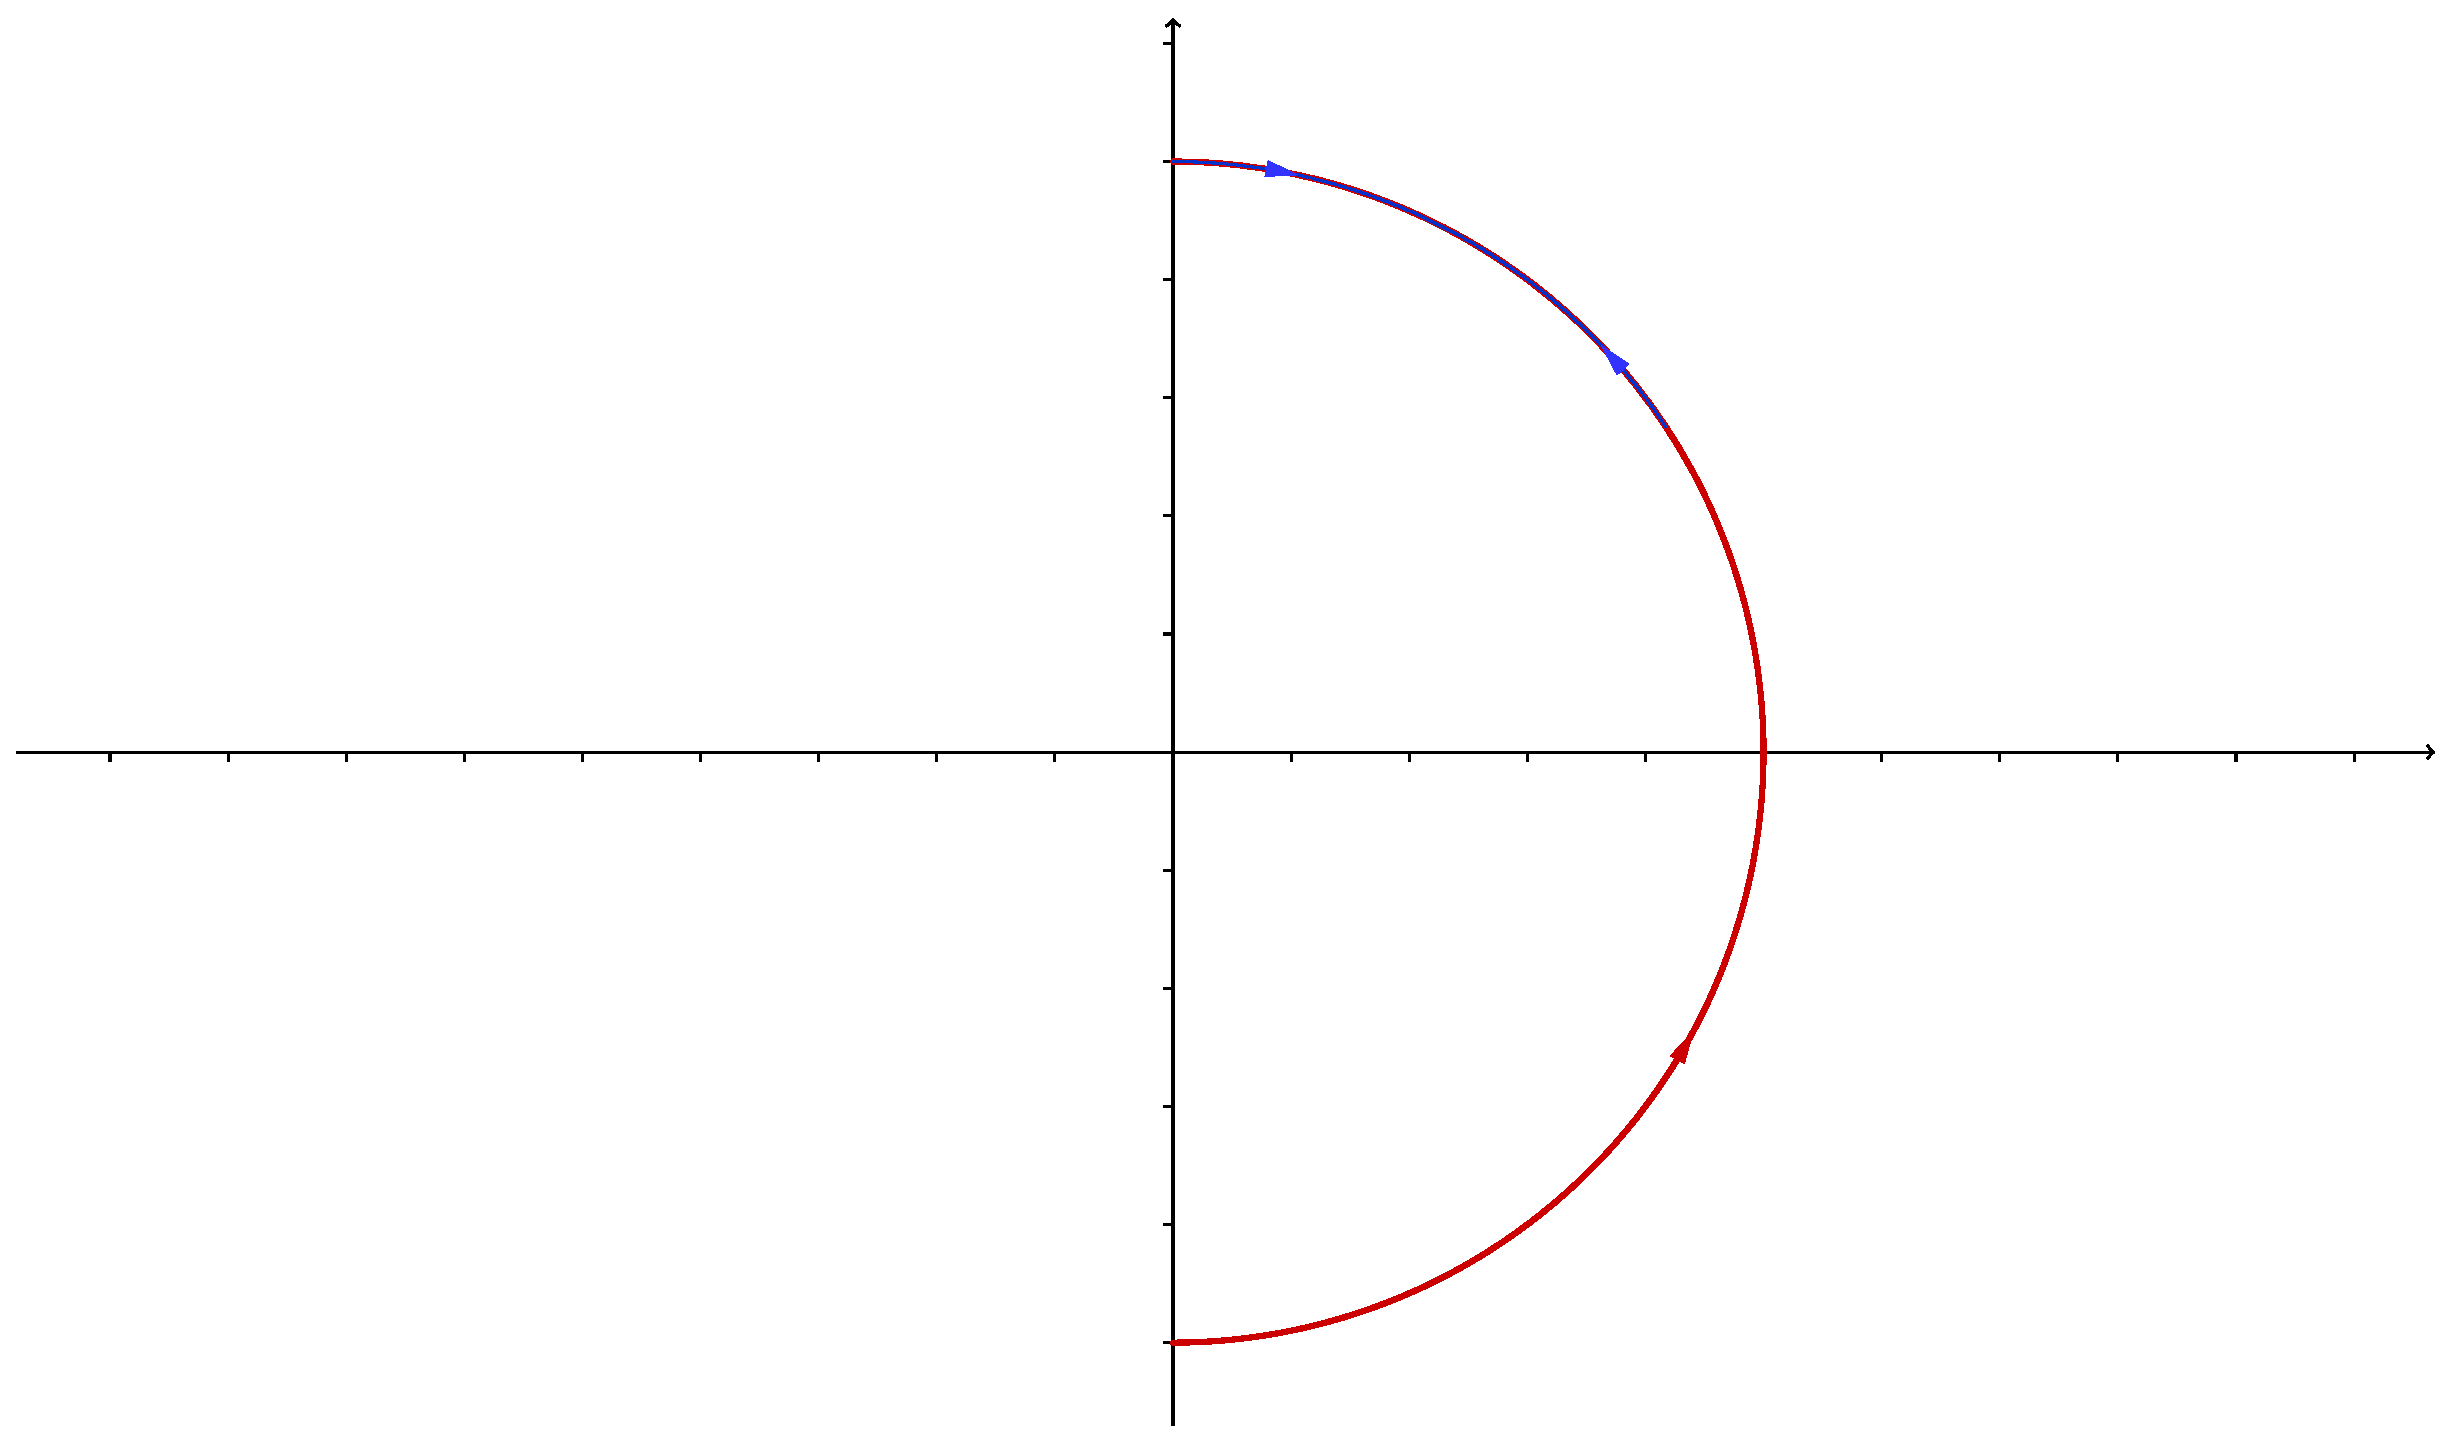
\includegraphics[width=0.5\textwidth]{Figures/Topologicalindex/topindex}  
\caption{In red (blue) $(h_x(k),h_z(k))$ is plotted as function of $k\in \{0, \infty\}$ for $\mu > 0$ ($\mu < 0$). Notice that for $\mu < 0$ the curve starts and ends at the north pole.}  
\label{fig.hhatplot}  
\end{center}    
\end{figure}

It is then clear, that as long as there is an energy gap, $\hat{h}(k)$ is well defined. Since $E_{F,k=0} = |\mu|$, we see that the energy is gapped exactly when $\mu \neq 0$. Finally, since $\Delta_{k=0} = 0$, we notice that: 
\begin{equation}
\hat{h}(k=0) = -\text{sgn}(\mu)\hat{z} = p_0\hat{z}, \hspace{0.5cm} \hat{h}(k=\infty) = \hat{z} = p_{\infty}\hat{z},
\label{eq.hhatk0kinfty}
\end{equation}
where $\text{sgn}$ denotes the sign function. The idea is then, that we can specify a number $\nu \in \{-1,1\}$ by:
\begin{equation}
\nu = p_0p_{\infty} = -\text{sgn}(\mu).
\label{eq.topinvnudefition}
\end{equation}
The claim is, that we have hereby defined a topological index, which specifies two states, that cannot be deformed into each other without closing the energy gap. Graphically this is clear from figure \ref{fig.hhatplot}. In red (blue) I have plotted the behaviour of $\hat{h}$ for $\mu > 0$ ($\mu < 0$), omitting the zero component $h_y$. For $\mu > 0$ we see, that we go from the south pole to the north pole as $k$ goes from $0$ to $\infty$. For $\mu < 0$ on the other hand, we see that $\hat{h}(k)$ starts out at the north pole, then goes somewhat along the circle arc before returning to the north pole. This is of course the same behaviour as written in equation \eqref{eq.hhatk0kinfty}. It is then clear, that there is no way of continuously deforming one map to the other. Further, we notice that the mapping becomes ill-defined exactly when $\mu = 0$. This is also evident from the appearance of $\text{sgn}(\mu)$ in $\nu$. We notice, that since $\mu(T) \to -\infty$ and $\Delta_k(T)\to 0$ for $T\to \infty$, the $\mu < 0$ phase is connected continously to the normal phase. Hence, the normal phase, and thereby also the vacuum, is associated with $\nu = 1$. 

For $T = 0$ the normal phase has $\mu = \epsilon_{F,0} > 0$. We can hereby distinguish between two regimes. The first is the weak coupling regime. The pairing does not significantly alter the chemical potential: $\mu(T=0) > 0$. Hereby $\nu = -1$ and the ground state is topologically \textit{non}-trivial. The second is the strong coupling regime, where $\mu(T = 0) < 0$, $\nu = 1$ and the ground state is topologically trivial. This is in complete harmony with the findings in \cite{Alicea} for the Kitaev chain.\footnote{In the article by Alicea the fermions sit in a lattice, but the physical properties are essentially the same.}

We are only investigating the weak coupling regime, even with $\mu \approx \epsilon_{F,0}$. From the above arguments, this means, that we have found a ground state with $\nu = -1$. So far, we have investigated the bulk properties of the superfluid by imposing cyclic boundary conditions. Imagine it now as a wire with open ends. This means, that there are junctions at the ends between a $\nu = -1$ (the superfluid wire) and a $\nu = 1$ state (the vacuum). It also means, that when we spatially follow the transition between the two phases, the wire and the vacuum, $\nu$ has to change its value abrubtly at the boundary. Hence, the energy gap has to dramatically drop to $0$ at the boundary. 

The interesting question is now: are there states that are topologically protected? More precisely, we are asking, whether there exist low energy states, that can only be removed by breaking the symmetries of the system. The answer lies in the build in particle-hole symmetry of the Hamiltonian. As we saw in section \ref{sec.SymmetriesTRandPH} we have a particle-hole symmetry $\mathcal{C} = \sigma_1 K$, with $K$ being the complex conjugation operator. Hereby $\mathcal{C}\mathcal{H}_{FF,k} = -\mathcal{H}_{FF,-k}\mathcal{C}$. Let us assume, that we have a single particle energy solution in $k$: $\mathcal{H}_{FF,k}\ket{\psi_k} = E_k\ket{\psi_k}$. We hereby directly get:
\begin{equation}
E_k\mathcal{C}\ket{\psi_k} = \mathcal{C}\mathcal{H}_{FF,k}\ket{\psi_k} = -\mathcal{H}_{FF,-k}\mathcal{C}\ket{\psi_k} \Rightarrow \mathcal{H}_{FF,-k}\left(\mathcal{C}\ket{\psi_k}\right) = -E_k\left(\mathcal{C}\ket{\psi_k}\right).
\end{equation}
This shows, that if $\ket{\psi_k}$ has the energy $E_k$, then $\mathcal{C}\ket{\psi_k}$ has the energy $-E_k$. In other words for every positive energy solution there is also a negative one, as is shown to the left in figure \ref{fig.edgestates}. The bulk spectrum is here indicated by a solid line above the bulk gap $\min_k[E_{F,k}]$ and mirrored in $E = 0$. Now suppose that we introduce a perturbation, that respects the particle-hole symmetry. The energies therefore still come in plus/minus pairs, but apart from that the energies can change. Hence, we can perturb any low energy state with $E \neq 0 $ away. This is indicated in the figure by the black dots and arrows. However, the \textit{single} state at $E = 0$ remains exactly there, because if it moved either up or down, there would not be the plus/minus symmetry in the energies. This leads to an energy spectrum, which is \textit{robust} against symmetry-conserving perturbations with the continuum above the bulk gap and a \textit{single} zero energy edge state as indicated in figure \ref{fig.edgestates}. 

With no energy cost edge states at the ends of the wire can hereby emerge and are robust to symmetry-conserving perturbations. This phenomenon is known as the bulk-edge correspondence principle, since it connects bulk effects, $\nu = -1$, to an edge effect (the edge states). As is indicated to the right in figure \ref{fig.edgestates}, the state has to be localised on the boundaries. The reason is, that all bulk states are already occupied, and so a zero energy bulk state is not available. 

\begin{figure}
\center
\begin{tikzpicture}
\draw[|->, thick] (0, 0) -- (0,  2) node[above]{$E$};
\draw[-, thick]   (0, 0) -- (0, -2);
\node at (-0.4, 0) {$0$};

\draw[-, dashed] (0, 1)--(1, 1);
\draw[-, thick] (-0.1, 1)--(0.1, 1);
\node at (-1.17,1) {$\min_k[E_{F,k}]$};

\draw[-, dashed] (0, -1)--(1, -1);
\draw[-, thick] (-0.1, -1)--(0.1, -1);
\node at (-1.35,-1) {$-\min_k[E_{F,k}]$};

\draw[-, ultra thick] (1, 1)--(1, 2);
\draw[-, ultra thick] (1, -1)--(1, -2);
\node[red] at (1, 0) {\textbullet};

\node at (1, 0.5) {\textbullet};
\draw[->] (1, 0.5) --  (1,  1);
\node at (1, -0.5) {\textbullet};
\draw[->] (1, -0.5) -- (1, -1);

\draw[-, dashed] (0,0.01) --(1,0.01);

\node at (3, -0.4) {$0$};
\node at (8, -0.4) {$\mathcal{L}$};
\draw[|->, thick ] (3,0) -- (9,0) node[right]{$x$};

\draw[-, ultra thick ] (3,0) -- (8,0);
\draw[scale=0.5,domain=-1:1,smooth,variable=\x,red] plot ({\x + 6},{ 3 * exp{- 10 * \x*\x}});
\draw[scale=0.5,domain=-1:1,smooth,variable=\x,red] plot ({\x + 16},{ 3 * exp{- 10 * \x*\x}});
\end{tikzpicture}
\caption{To the left the energy spectrum is sketched. Because of the particle-hole symmetry, there is a negative energy state for every positive. There is a continuum of states above $\min_k[E_{F,k}]$ and below $-\min_k[E_{F,k}]$. At the boundary of the wire the gap closes, but the particle-hole symmetry only protects the single state at $E = 0$, indicated by the red dot. The corresponding wave function is sketched to the right.}
\label{fig.edgestates}
\end{figure}

We can now also clarify, what is meant by the term \textit{topological} superfluid. The above mentioned effects are called topological, because the classification with respect to the symmetries $T,C$ and $S$ is deeply connected to topology; specifically the study of manifolds. This is of abstract parameter spaces, and so the naming as such does not originate from the fact, that the edge states are located at specific places geometrically, as one might be led to believe.  

\section{The Chern-Simons invariant and the Wilson loop}
\label{sec.CS1}
In this section we calculate the Chern-Simons topological invariant of the system and in turn the gauge independent Wilson loop. It is based on the article \cite{Ryu.Topology}. We do not anticipate any breaking of time reversal symmetry. The topological index is therefore to be found in the integers, $\mathbb{Z}$. We will work with $\Delta_k$ real. The calculation in this section is more rigorous but also less intuitive than the one in the previous section.

The Chern-Simons invariant is generally a half integer: $\dots, -3/2, -1, -1/2, 0, 1/2, \dots$. The topological index, generally called the winding number, is twice the Chern-Simons invariant, hence an integer. This gives us the desired topological index in $\mathbb{Z}$. In one spatial dimension the Chern-Simons invariant is generally defined as:
\begin{equation}
\text{CS}_1 = \frac{i}{2\pi}\int_{\text{BZ}}dk \; \text{tr}\left[\mathcal{A}_k\right], \nonumber
\end{equation}
where BZ is short for the first Brillouin zone, and $\mathcal{A}_k$ is the socalled Berry connection. In the literature the Chern-Simons invariant is also referred to as the (total) polarisation. This naming has a physical reasoning in electronic topological insulators, because it is actually a measure of the charge polarisation as a consequence of the edge states \cite{FuKane2006}. Since there are no charge carriers in our system, we will not use this naming. Now let $\ket{e^{-}_k}$ be the eigenvector to $\mathcal{H}_{FF,k}$ with eigenvalue $-E_{F,k}$. The Berry connection is then in this case defined as:
\begin{equation}
\mathcal{A}_k = \bra{e^{-}_k}\partial_k\ket{e^{-}_k}. \nonumber
\end{equation}
The result of Chern-Simons theory is then, that the Chern-Simons invariant is a topological invariant. By this, it is meant, that it characterizes different topological phases, that can only change when the energy gap closes. It turns out that the calculation in this scenario is easier in a different basis, than the one we have been working in so far. Let us therefore shortly investigate the influence of basis on the Berry connection. In a different basis we have: $\tilde{\mathcal{H}}_{FF,k} = U\mathcal{H}_{FF,k}U^\dagger$, where $U$ is some unitary matrix not depending on $k$. If $\mathcal{H}_{FF,k}\ket{e^{-}_k} = -E_{F,k}\ket{e^{-}_k}$, the eigenvector in the new basis with negative eigenvalue is $\ket{\tilde{e}^{-}_k} = U\ket{e^{-}_k}$. The corresponding Berry connection is:
\begin{equation}
\tilde{\mathcal{A}}_k = \bra{\tilde{e}^{-}_k}\partial_k\ket{\tilde{e}^{-}_k} = \bra{e^{-}_k}U^\dagger\partial_k U\ket{e^{-}_k} = \bra{e^{-}_k}\partial_k\ket{e^{-}_k} = \mathcal{A}_k, \nonumber 
\end{equation}
whereby the Berry connection and hereby the Chern-Simons invariant is unaltered. This is of course very reasonable; a topological invariant should not depend on the chosen basis. We now make a specific choice for $U$:
\begin{equation}
U = \text{e}^{i\sigma_1 \frac{3\pi}{4}} = \frac{1}{\sqrt{2}}\left(-\mathbb{I} + i\sigma_1\right). \nonumber 
\end{equation}
This transformation amounts to letting $(\sigma_1, \sigma_2, \sigma_3) \overset{U}{\to} (\sigma_1, \sigma_3, -\sigma_2)$. Since $\mathcal{H}_{FF,k} = \Delta_k\sigma_1 + \varepsilon_k\sigma_3$, in the new basis we get: $\tilde{\mathcal{H}}_{FF,k} = U\mathcal{H}_{FF,k}U^\dagger = \Delta_k\sigma_1 - \varepsilon_k\sigma_2$. The reason for changing basis is, that the eigenvectors are simpler. Explicitly:
\begin{equation}
\ket{\tilde{e}^{-}_k} = \frac{1}{\sqrt{2}}\begin{bmatrix} -\frac{\Delta_k + i \varepsilon_k}{E_{F,k}} \\ 1 \end{bmatrix}. \nonumber 
\end{equation}
With this and a bit of calculating the Berry connection becomes:
\begin{equation}
\mathcal{A}_k = \bra{\tilde{e}^{-}_k}\partial_k\ket{\tilde{e}^{-}_k} = -\frac{i}{2E^2_{F,k}}(\varepsilon_k\partial_k\Delta_k - \Delta_k \partial_k \varepsilon_k). \nonumber 
\end{equation}
Since the Brillouin zone is simply the entire axis, $k\in (-\infty, \infty)$, we get:
\begin{equation}
\text{CS}_1 = \frac{i}{2\pi}\int_{\text{BZ}} dk\; \text{tr}\left[\mathcal{A}_k\right] = \frac{1}{4\pi}\int_{-\infty}^{\infty} dk \;  \frac{\varepsilon_k\partial_k\Delta_k - \Delta_k \partial_k \varepsilon_k}{\varepsilon^2_k + \Delta^2_k} = \frac{1}{2\pi}\int_0^\infty dk \; \frac{\varepsilon_k\partial_k\Delta_k - \Delta_k \partial_k \varepsilon_k}{\varepsilon^2_k + \Delta^2_k}, 
\label{eq.CSinv1}
\end{equation}
where the last equality stems from the fact, that the integrand is even. The integrand has a primitive given by $-\arctan\left(\frac{\varepsilon_k}{\Delta_k}\right)$. Hence, the above is directly calculable:
\begin{align}
\text{CS}_1 &= - \frac{1}{2\pi} \left. \arctan\left(\frac{\varepsilon_k}{\Delta_k}\right)\right|^\infty_0 \overset{(*)}{=} -\frac{\text{sgn}(\Delta_{k>0})}{2\pi}\left(\frac{\pi}{2} - \lim_{a\to 0^{+}}\arctan\left(\frac{-\mu}{a}\right) \right) \nonumber \\
& = \left\{ \begin{matrix} -\frac{\text{sgn}(\Delta_{k>0})}{2}, & \mu > 0, \\ 0, & \mu < 0. \end{matrix} \right. 
\label{eq.CSinv2}
\end{align}
By $\text{sgn}(\Delta_{k>0})$ we mean the sign of $\Delta_k$ for $k > 0$. Two effects lead to the equality $(*)$. Firstly, $\arctan(x) \to \pi/2$ for $x \to \infty$. $\text{sgn}(\Delta_{k>0})$ appears, since if $\Delta_k$ is negative for $k > 0$, the argument $\frac{\varepsilon_k}{\Delta_k}$ goes to $-\infty$ for $k \to \infty$. Secondly, since $\Delta_{k=0} = 0$ the evaluation in $k = 0$ can be performed by the written limit of $a \to 0^+$. This shows, that the Chern-Simons invariant is \textit{not} invariant under gauge transformations, e.g. $\Delta_k \to - \Delta_k$. Since the two nonzero Chern-Simons invariants are related by a gauge transformation, they are equivalent. To account for this, we compute the \textit{gauge independent} Wilson loop $W_1$. We get: 
\begin{equation}
W_1 = \text{e}^{2\pi i \text{CS}_1} = -\text{sgn}(\mu). 
\end{equation}
We have $\Delta_k = 0$ in the normal phase, which is the topologically trivial phase. It therefore follows from equation \eqref{eq.CSinv1}, that $\text{CS}_1 = 0$ and hence $W_1 = 1$ for the trivial phase. This means, that $W_1 = -1$ is the (only) topological (non-trivial) phase. We also see, that the condition is exactly the same as the one found in the previous section. It is however quite satisfying to see, that we can come to this result in a more rigorous manner, also not assuming any brokenness of the time reversal symmetry. The edge states analysis of the previous section is unaltered in the present context.  

\vspace{1cm}
The question now becomes the following. Is it possible to make a simple physical change of the system, that allows us to observe a topological phase transition? The proposal is to put in a \textit{second} wire parallel to the already studied. By doing this we get two kinds of interactions. The first is the \textit{intra}wire interaction, the interaction internally in each wire, which we have already studied in detail. The second is the \textit{inter}wire interaction, the interaction between the two wires. Further, we get an extra parameter, namely the distance $d$ between the wires. It will allow us to study the transition between intrawire and interwire dominated interactions, and further what effect the topology has on the transition. This is the subject of part III of this thesis. 


% Chapter 7

\chapter{Two wires, induced interaction} % Main chapter title

\label{Chapter8} % For referencing the chapter elsewhere, use \ref{Chapter8} 

\lhead{Chapter 8. \emph{2 wires, induced interaction}} % This is for the header on each page - perhaps a shortened title

%----------------------------------------------------------------------------------------
In the chapter we will introduce a second wire parallel to the first one already studied. The aim here is to calculate the additional (interwire) induced interaction between the wires. The approach mirrors chapter \ref{Chapter3}. For this reason we will not go in as much detail in the present chapter.
\section{The effective Bose-Fermi interaction} 
As for the single wire the effective Bose-Fermi interaction is modelled by $V(\mathbf{r}) = g_{BF}\delta(\mathbf{r})$. To begin with, this gives the same expression for the interaction Hamiltonian between the bosons (B) and the fermions (F):
\begin{equation}
H_{BF}^\text{int} = g_{BF}\int d^3 r \hat{\psi}_F^\dagger(\mathbf{r}) \hat{\psi}_B^\dagger(\mathbf{r})\hat{\psi}_B(\mathbf{r})\hat{\psi}_F(\mathbf{r}).
\end{equation}

The difference now is, that we trap the fermions along \textit{two} wires. Let the first one be along the $x$-axis, the second at $z=d, y=0$. The fermions are trapped in a harmonic trap with trapping frequency $\omega_t$. In this connection we have two central assumptions. The first is the same as for the single wire: we require, that the fermions are trapped in the ground state with respect to the perpendicular directions. The second assumption is, that the distance between the wires is much larger than the trapping width of the wires $l_t = \frac{1}{\sqrt{m_F\omega_t}}$. Hence, $l_t/d \gg 1$. This is done, so that we can actually talk about distinguishable wires of fermions. This leads to the following expansion in momentum eigenstates:
\begin{equation}
\psi_F(x,\mathbf{r}_\perp) = \frac{1}{\sqrt{\mathcal{L}}}\sum_p \text{e}^{ipx} \left[\phi_0(\mathbf{r}_\perp) f_{1,p} + \phi_0(\mathbf{r}_\perp-\mathbf{d}) f_{2,p}\right], \hspace{0.5cm} \psi_B(\mathbf{r}) = \frac{1}{\sqrt{\mathcal{V}}}\sum_{\mathbf{k}} \text{e}^{i\mathbf{k}\cdot \mathbf{r}} b_\mathbf{k}, 
\end{equation}  
with $\phi_0(\mathbf{r}_\perp) = \frac{1}{\sqrt{\pi}l_t}\exp\left(-\frac{r_\perp^2}{2l_t^2}\right)$ the ground state with respect to the perpendicular directions. $f^\dagger_{j,p}$ therefore creates a fermion in wire $j$ with momentum $p$. We assume, that the wires are truly distinguishable. This means that all anticommutators like $\{f_{1,p}, f^\dagger_{2,p'}\}$ vanish. Inserting these expressions into $H_{BF}^\text{int}$ yields in total four terms. However, the cross terms where a fermion is annihilated in one wire and created in the other are proportional to the integral:
\begin{equation}
\int d^2 r_\perp \phi_0(\mathbf{r}_\perp)\phi_0(\mathbf{r}_\perp-\mathbf{d}) = 0. 
\end{equation}
The integral is negligible, because by assumption $l_t/d \gg 1$. A similar analysis to the one in chapter \ref{Chapter3} then yields for the diagonal terms:
\begin{align}
H_{BF}^\text{int} = \frac{g_{BF}}{\mathcal{V}}\sum_{p_1,p_2,q} \sum_{\mathbf{k}_\perp, \mathbf{k}_\perp'} & \text{e}^{-\frac{l_t^2}{4}(\mathbf{k}_\perp - \mathbf{k}_\perp')^2}\left[ f^\dagger_{1,p_2-q} b^\dagger_{p_1+q, \mathbf{k}_\perp'} b_{p_1,\mathbf{k}_\perp}f_{1,p_2} + \right. \nonumber \\
& \left. \text{e}^{i(\mathbf{k}_\perp - \mathbf{k}_\perp')\cdot \mathbf{d}}f_{2,p_2-q}^\dagger b_{p_1+q, \mathbf{k}_\perp'}^\dagger b_{p_1,\mathbf{k}_\perp}f_{2,p_2} \right].
\end{align}

This shows, that a scattering event in wire 1 is associated with the factor $g_{BF} \text{e}^{-\frac{l_t^2}{4}(\mathbf{k}_\perp - \mathbf{k}_\perp')^2}$ as before, and that the corresponding scattering in wire 2 has an extra factor of $\text{e}^{i(\mathbf{k}_\perp - \mathbf{k}_\perp')\cdot \mathbf{d}}$. 

\section{The 1D-3D induced interaction}
The intrawire induced interaction is (of course) the same as the one for the single line. Referring to equation \ref{eq.VFFindXBEC} this means, that:
\begin{equation}
V_{FF,11}^\text{ind}(q,i\omega_q) = V_{FF,22}^\text{ind}(q,i\omega_q) = g_{BF}^2\int\frac{d^2k_\perp}{(2\pi)^2}\; \chi_\text{BEC}(q,\mathbf{k}_\perp,i\omega_q)\text{e}^{-\frac{l_t^2}{2}k_\perp^2}, 
\label{eq.VFF1122indXBEC} 
\end{equation}
with $\chi_\text{BEC}(\mathbf{k},i\omega_q) = \frac{k^2}{m_B}\frac{n_B}{(i\omega_q)^2-E_{B,k}^2}$ the density-density correlation function. The index $11$ ($22$) indicates, that the interaction is between two fermions in wire 1 (wire 2). One might wonder what happens to the extra factor of $\text{e}^{i(\mathbf{k}_\perp - \mathbf{k}_\perp')\cdot \mathbf{d}}$. The incoming boson is associated with a factor of $\text{e}^{i\mathbf{k}_\perp\cdot \mathbf{d}}$. However, the outgoing is associated with a factor of $\text{e}^{-i\mathbf{k}_\perp\cdot \mathbf{d}}$, and so these cancel. This is as it should be, because the intrawire interaction in the two wires should be the same!

The additional scenario now is, that there is also an interwire induced interaction, which we will denote $V_{FF,12}^\text{ind}(q,i\omega_q)$. The preceding section shows, that the calculation of this induced interaction is analogous to the above, but with the additional factor of $\text{e}^{i\mathbf{k}_\perp\cdot \mathbf{d}}$ from scattering in the second wire. Explicitly the Feynman diagrams of importance are shown in figure \ref{fig.interwirefeynmandiagrams}. They have the same form as the ones in figure \ref{fig.feynmandiagrams} with the (obvious) caveat, that the induced interaction is now between a fermion in wire 1 and a fermion in wire 2. Hence,
\begin{equation}
V_{FF,12}^\text{ind}(q,i\omega_q) = g_{BF}^2\int\frac{d^2k_\perp}{(2\pi)^2}\; \chi_\text{BEC}(q,\mathbf{k}_\perp,i\omega_q)\text{e}^{-\frac{l_t^2}{2}k_\perp^2}\text{e}^{i\mathbf{k}_\perp\cdot \mathbf{d}}. 
\label{eq.VFF12indXBEC} 
\end{equation}

\begin{figure}
\begin{tikzpicture}[scale=0.25]
  \begin{feynman}[small]
    \vertex (number1) {\( (1) \)};
    \vertex [above left=of number1] (fermion1) {\( 1, \tilde{p}_1 \)};
    \vertex [above right=of fermion1] (a);
    \vertex [below right=of a] (fermion2) {\(1, \tilde{p}_1+\tilde{q}\)}; 
    \vertex [above=of a] (b);
    \vertex [left=of b] (boson1) {\( \sqrt{n_B} \)}; 
    \vertex [above= of b] (c);
    \vertex [right= of c] (boson2) {\( \sqrt{n_B} \)};
    \vertex [above= of c] (d);
    \vertex [above left=of d] (f3) {\(2, \tilde{p}_2\)};
    \vertex [above right=of d] (f4) {\(2, \tilde{p}_2-\tilde{q}\)};
 
    \diagram* {
      (number1) -- [opacity=0.0] (fermion1) -- [fermion] (a) -- [fermion] (fermion2),
      (a) -- [photon, edge label'=\(g_{BF}\)] (b),
      (b) -- [dashed] (boson1),
      (b) -- [blue, fermion, edge label' = {\(-\tilde{q}, \mathbf{k}_\perp \)}] (c),
      (c) -- [dashed] (boson2),
      (c) -- [photon, edge label'=\(g_{BF}\)] (d),
      (d) -- [anti fermion] (f3),
      (d) -- [fermion] (f4)
    };
  \end{feynman}
\end{tikzpicture}
\begin{tikzpicture}
  \begin{feynman}[small]
    \vertex (number2) {\( (2) \)};
    \vertex [above left=of number2] (fermion1) {\(1, \tilde{p}_1 \)};
    \vertex [above right=of fermion1] (a);
    \vertex [below right=of a] (fermion2) {\(1, \tilde{p}_1+\tilde{q}\)}; 
    \vertex [above=of a] (b);
    \vertex [left=of b] (boson1) {\( \sqrt{n_B} \)}; 
    \vertex [above= of b] (c);
    \vertex [right= of c] (boson2) {\( \sqrt{n_B} \)};
    \vertex [above= of c] (d);
    \vertex [above left=of d] (f3) {\(2, \tilde{p}_2\)};
    \vertex [above right=of d] (f4) {\(2, \tilde{p}_2-\tilde{q}\)};
 
    \diagram* {
      (number2) -- [opacity=0.0] (fermion1) -- [fermion] (a) -- [fermion] (fermion2),
      (a) -- [photon, edge label'=\(g_{BF}\)] (b),
      (b) -- [dashed] (boson1),
      (b) -- [blue, anti fermion, edge label' = {\(\tilde{q}, \mathbf{k}_\perp \)}] (c),
      (c) -- [dashed] (boson2),
      (c) -- [photon, edge label'=\(g_{BF}\)] (d),
      (d) -- [anti fermion] (f3),
      (d) -- [fermion] (f4)
    };
  \end{feynman}
\end{tikzpicture}
\begin{tikzpicture}
  \begin{feynman}[small]
    \vertex (number3) {\( (3) \)};
    \vertex [above left=of number3] (fermion1) {\(1, \tilde{p}_1 \)};
    \vertex [above right=of fermion1] (a);
    \vertex [below right=of a] (fermion2) {\(1, \tilde{p}_1+\tilde{q}\)}; 
    \vertex [above=of a] (b);
    \vertex [left=of b] (boson1) {\( \sqrt{n_B} \)}; 
    \vertex [above= of b] (c);
    \vertex [right= of c] (boson2) {\( \sqrt{n_B} \)};
    \vertex [above= of c] (d);
    \vertex [above left=of d] (f3) {\(2, \tilde{p}_2\)};
    \vertex [above right=of d] (f4) {\(2, \tilde{p}_2-\tilde{q}\)};
 
    \diagram* {
      (number3) -- [opacity=0.0] (fermion1) -- [fermion] (a) -- [fermion] (fermion2),
      (a) -- [photon, edge label'=\(g_{BF}\)] (b),
      (b) -- [dashed] (boson1),
      (b) -- [blue, majorana, edge label' = {\(\tilde{q}, \mathbf{k}_\perp \)}] (c),
      (c) -- [dashed] (boson2),
      (c) -- [photon, edge label'=\(g_{BF}\)] (d),
      (d) -- [anti fermion] (f3),
      (d) -- [fermion] (f4)
    };
  \end{feynman}
\end{tikzpicture}
\begin{tikzpicture}
  \begin{feynman}[small]
    \vertex (number4) {\( (4) \)};
    \vertex [above left=of number4] (fermion1) {\(1, \tilde{p}_1 \)};
    \vertex [above right=of fermion1] (a);
    \vertex [below right=of a] (fermion2) {\(1, \tilde{p}_1+\tilde{q}\)}; 
    \vertex [above=of a] (b);
    \vertex [left=of b] (boson1) {\( \sqrt{n_B} \)}; 
    \vertex [above= of b] (c);
    \vertex [right= of c] (boson2) {\( \sqrt{n_B} \)};
    \vertex [above= of c] (d);
    \vertex [above left=of d] (f3) {\(2, \tilde{p}_2\)};
    \vertex [above right=of d] (f4) {\(2, \tilde{p}_2-\tilde{q}\)};
 
    \diagram* {
      (number3) -- [opacity=0.0] (fermion1) -- [fermion] (a) -- [fermion] (fermion2),
      (a) -- [photon, edge label'=\(g_{BF}\)] (b),
      (b) -- [dashed] (boson1),
      (b) -- [blue, anti majorana, edge label' = {\(\tilde{q}, \mathbf{k}_\perp \)}] (c),
      (c) -- [dashed] (boson2),
      (c) -- [photon, edge label'=\(g_{BF}\)] (d),
      (d) -- [anti fermion] (f3),
      (d) -- [fermion] (f4)
    };
  \end{feynman}
\end{tikzpicture}
\caption{Feynman diagrams for the induced interaction between the wires. Since the interaction is weak, we can neglect all other Feynman diagrams than (1)-(4). Diagrams (1) and (2) stems from the normal Green's function $G_{11}$. Diagrams (3) and (4) stems from the anormalous Green's function $G_12$.} \label{fig.interwirefeynmandiagrams}
\end{figure}


We will only investigate the $l_t \to 0$ and $\omega_q = 0$ limit. The reasoning behind the $\omega_q = 0$ limit is the same as for the single wire. See \ref{sec.RetardationEffects} for details. Further, it is already here possible to take the $l_t \to 0$ limit in contrast to the intrawire interaction case. By rewriting the above integral, we get:
\begin{align}
V_{FF,12}^\text{ind}(q,0) &= -\frac{n_Bg_{BF}^2m_B}{\pi^2}\int_0^\infty d k_\perp \; \frac{k_\perp}{k_\perp^2 + q^2 + 2/\xi^2} \int_0^{2\pi} d\theta \; \text{e}^{ik_\perp d\cos(\theta)} \nonumber \\
						  &= -\frac{2n_Bg_{BF}^2m_B}{\pi}\int_0^\infty d k_\perp \; \frac{k_\perp J_0(k_\perp d)}{k_\perp^2 + q^2 + 2/\xi^2},
\label{eq.secondwireinducedinteractionmomentumspaceintegralexpression}
\end{align}
with $J_0$ the zero order Bessel function of the first kind. This form of the potential is not terrible illuminating. In stead let us take the Fourier transform to get the induced interaction in real space, $\tilde{V}^\text{ind}_{FF}(x,0)$. Write $\mathbf{r} = (x,\mathbf{d})$ and $\mathbf{k} = (q,\mathbf{k}_\perp)$. We then get the expression:
\begin{align}
\tilde{V}_{FF,12}^\text{ind}(x,0) &= \int \frac{dq}{2\pi} \; \text{e}^{iqx} V_{FF,12}^\text{ind}(q,0) = -4n_Bg^2_{BF}m_B\int \frac{d^3k}{(2\pi)^3} \frac{\text{e}^{i\mathbf{k}\cdot \mathbf{r}}}{k^2 + 2/\xi^2} \nonumber \\
								  &= -\frac{n_Bg^2_{BF}m_B}{\pi} \frac{\text{e}^{-\sqrt{2(x^2+d^2)}/\xi}}{\sqrt{x^2+d^2}},
\end{align}
since we recognise the second expression as the Yukawa potential in momentum space with range $\xi/\sqrt{2}$. The interwire induced interaction is hereby shown to be the natural generalisation of the intrawire interaction found in chapter \ref{Chapter3}. This further enables us to get a closed form expression for the induced interaction in momentum space. Writing up the Fourier transform, we get:
\begin{equation}
V^\text{ind}_{FF,12}(q,0) = \int dx \; \text{e}^{-iqx}\tilde{V}^\text{ind}_{FF,12}(x,0) = 2\int_0^\infty \cos(qx)\tilde{V}^\text{ind}_{FF,12}(x,0), \nonumber 
\end{equation}
since the induced interaction is even in real space. Writing the variables in units of the range $\xi/\sqrt{2}$, we get:
\begin{equation}
V^\text{ind}_{FF,12}(\tilde{q},0) = -\frac{2n_Bg^2_{BF}m_B}{\pi}\int_0^\infty d\tilde{x} \cos(\tilde{q}\tilde{x})\frac{ \text{e}^{ -\sqrt{\tilde{x}^2+\tilde{d}^2} } }{\sqrt{\tilde{x}^2+\tilde{d}^2}} = -\frac{2n_Bg^2_{BF}m_B}{\pi}K_0\left(\tilde{d}\sqrt{\tilde{q}^2+1}\right), \nonumber
\end{equation}
where $K_0(x)$ is the modified Bessel function of the second kind of order zero. This calculation is done with the use of the Fourier cosine transform routine in Maple 16. The result is verified by comparing it graphically to the integral expression of equation \eqref{eq.secondwireinducedinteractionmomentumspaceintegralexpression}. Since $\tilde{q} = \frac{q\xi}{\sqrt{2}}, \tilde{d} = \frac{\sqrt{2}d}{\xi}$, we finally get:
 \begin{equation}
V^\text{ind}_{FF,12}(q,0) = -\frac{2n_Bg^2_{BF}m_B}{\pi}K_0\left(\sqrt{(qd)^2+\frac{2d^2}{\xi^2}}\right). 
\end{equation}
The fact, that we can express the induced interaction in terms of a known function is crucial for the feasibility of the later numerical analysis. 

\begin{figure} 
\begin{center}  
% GNUPLOT: LaTeX picture with Postscript
\begingroup
  \makeatletter
  \providecommand\color[2][]{%
    \GenericError{(gnuplot) \space\space\space\@spaces}{%
      Package color not loaded in conjunction with
      terminal option `colourtext'%
    }{See the gnuplot documentation for explanation.%
    }{Either use 'blacktext' in gnuplot or load the package
      color.sty in LaTeX.}%
    \renewcommand\color[2][]{}%
  }%
  \providecommand\includegraphics[2][]{%
    \GenericError{(gnuplot) \space\space\space\@spaces}{%
      Package graphicx or graphics not loaded%
    }{See the gnuplot documentation for explanation.%
    }{The gnuplot epslatex terminal needs graphicx.sty or graphics.sty.}%
    \renewcommand\includegraphics[2][]{}%
  }%
  \providecommand\rotatebox[2]{#2}%
  \@ifundefined{ifGPcolor}{%
    \newif\ifGPcolor
    \GPcolortrue
  }{}%
  \@ifundefined{ifGPblacktext}{%
    \newif\ifGPblacktext
    \GPblacktexttrue
  }{}%
  % define a \g@addto@macro without @ in the name:
  \let\gplgaddtomacro\g@addto@macro
  % define empty templates for all commands taking text:
  \gdef\gplbacktext{}%
  \gdef\gplfronttext{}%
  \makeatother
  \ifGPblacktext
    % no textcolor at all
    \def\colorrgb#1{}%
    \def\colorgray#1{}%
  \else
    % gray or color?
    \ifGPcolor
      \def\colorrgb#1{\color[rgb]{#1}}%
      \def\colorgray#1{\color[gray]{#1}}%
      \expandafter\def\csname LTw\endcsname{\color{white}}%
      \expandafter\def\csname LTb\endcsname{\color{black}}%
      \expandafter\def\csname LTa\endcsname{\color{black}}%
      \expandafter\def\csname LT0\endcsname{\color[rgb]{1,0,0}}%
      \expandafter\def\csname LT1\endcsname{\color[rgb]{0,1,0}}%
      \expandafter\def\csname LT2\endcsname{\color[rgb]{0,0,1}}%
      \expandafter\def\csname LT3\endcsname{\color[rgb]{1,0,1}}%
      \expandafter\def\csname LT4\endcsname{\color[rgb]{0,1,1}}%
      \expandafter\def\csname LT5\endcsname{\color[rgb]{1,1,0}}%
      \expandafter\def\csname LT6\endcsname{\color[rgb]{0,0,0}}%
      \expandafter\def\csname LT7\endcsname{\color[rgb]{1,0.3,0}}%
      \expandafter\def\csname LT8\endcsname{\color[rgb]{0.5,0.5,0.5}}%
    \else
      % gray
      \def\colorrgb#1{\color{black}}%
      \def\colorgray#1{\color[gray]{#1}}%
      \expandafter\def\csname LTw\endcsname{\color{white}}%
      \expandafter\def\csname LTb\endcsname{\color{black}}%
      \expandafter\def\csname LTa\endcsname{\color{black}}%
      \expandafter\def\csname LT0\endcsname{\color{black}}%
      \expandafter\def\csname LT1\endcsname{\color{black}}%
      \expandafter\def\csname LT2\endcsname{\color{black}}%
      \expandafter\def\csname LT3\endcsname{\color{black}}%
      \expandafter\def\csname LT4\endcsname{\color{black}}%
      \expandafter\def\csname LT5\endcsname{\color{black}}%
      \expandafter\def\csname LT6\endcsname{\color{black}}%
      \expandafter\def\csname LT7\endcsname{\color{black}}%
      \expandafter\def\csname LT8\endcsname{\color{black}}%
    \fi
  \fi
    \setlength{\unitlength}{0.0500bp}%
    \ifx\gptboxheight\undefined%
      \newlength{\gptboxheight}%
      \newlength{\gptboxwidth}%
      \newsavebox{\gptboxtext}%
    \fi%
    \setlength{\fboxrule}{0.5pt}%
    \setlength{\fboxsep}{1pt}%
\begin{picture}(7200.00,5040.00)%
    \gplgaddtomacro\gplbacktext{%
      \csname LTb\endcsname%
      \put(682,1188){\makebox(0,0)[r]{\strut{}$-4$}}%
      \csname LTb\endcsname%
      \put(682,2030){\makebox(0,0)[r]{\strut{}$-2$}}%
      \csname LTb\endcsname%
      \put(682,2872){\makebox(0,0)[r]{\strut{}$0$}}%
      \csname LTb\endcsname%
      \put(682,3713){\makebox(0,0)[r]{\strut{}$2$}}%
      \csname LTb\endcsname%
      \put(682,4555){\makebox(0,0)[r]{\strut{}$4$}}%
      \csname LTb\endcsname%
      \put(877,484){\makebox(0,0){\strut{}$-10$}}%
      \csname LTb\endcsname%
      \put(2343,484){\makebox(0,0){\strut{}$-5$}}%
      \csname LTb\endcsname%
      \put(3809,484){\makebox(0,0){\strut{}$0$}}%
      \csname LTb\endcsname%
      \put(5274,484){\makebox(0,0){\strut{}$5$}}%
      \csname LTb\endcsname%
      \put(6740,484){\makebox(0,0){\strut{}$10$}}%
    }%
    \gplgaddtomacro\gplfronttext{%
      \csname LTb\endcsname%
      \put(176,2871){\rotatebox{-270}{\makebox(0,0){\strut{}$2m_F/k_F W_{	ext{ind}}(k, k_F)$}}}%
      \put(3808,154){\makebox(0,0){\strut{}$k / k_F$}}%
      \csname LTb\endcsname%
      \put(4565,4803){\makebox(0,0)[l]{\strut{}$k_Fd = 0.720$}}%
      \csname LTb\endcsname%
      \put(4565,4583){\makebox(0,0)[l]{\strut{}$k_Fd = 0.735$}}%
      \csname LTb\endcsname%
      \put(4565,4363){\makebox(0,0)[l]{\strut{}$k_Fd = 0.750$}}%
      \csname LTb\endcsname%
      \put(4565,4143){\makebox(0,0)[l]{\strut{}$k_Fd = 0.765$}}%
      \csname LTb\endcsname%
      \put(4565,3923){\makebox(0,0)[l]{\strut{}$k_Fd = 0.775$}}%
    }%
    \gplbacktext
    \put(0,0){\includegraphics{InducedInteraction}}%
    \gplfronttext
  \end{picture}%
\endgroup
  
\caption{The zero frequency potential $V_{FF,12}^\text{ind}(q,0)$ plotted as a function of $q$. The induced interaction is seen to increase with decreasing distance $d$. Parameters: $(n_Ba_B^3)^{1/3} = 0.01$, $(n_Ba_{BF}^3)^{1/3} = 0.1$, $l_t = 0$, $\frac{m_B}{m_F} = 7/40$, $\frac{n_F}{n_B^{1/3}} = 0.215$, $\frac{m_F^2}{m_B^2}\frac{n_B}{n_F^3} k_Fa_B = 22.10$.}  
\label{fig.VFF12indq}  
\end{center}    
\end{figure}

\begin{figure} 
\begin{center}  
% GNUPLOT: LaTeX picture with Postscript
\begingroup
  \makeatletter
  \providecommand\color[2][]{%
    \GenericError{(gnuplot) \space\space\space\@spaces}{%
      Package color not loaded in conjunction with
      terminal option `colourtext'%
    }{See the gnuplot documentation for explanation.%
    }{Either use 'blacktext' in gnuplot or load the package
      color.sty in LaTeX.}%
    \renewcommand\color[2][]{}%
  }%
  \providecommand\includegraphics[2][]{%
    \GenericError{(gnuplot) \space\space\space\@spaces}{%
      Package graphicx or graphics not loaded%
    }{See the gnuplot documentation for explanation.%
    }{The gnuplot epslatex terminal needs graphicx.sty or graphics.sty.}%
    \renewcommand\includegraphics[2][]{}%
  }%
  \providecommand\rotatebox[2]{#2}%
  \@ifundefined{ifGPcolor}{%
    \newif\ifGPcolor
    \GPcolortrue
  }{}%
  \@ifundefined{ifGPblacktext}{%
    \newif\ifGPblacktext
    \GPblacktexttrue
  }{}%
  % define a \g@addto@macro without @ in the name:
  \let\gplgaddtomacro\g@addto@macro
  % define empty templates for all commands taking text:
  \gdef\gplbacktext{}%
  \gdef\gplfronttext{}%
  \makeatother
  \ifGPblacktext
    % no textcolor at all
    \def\colorrgb#1{}%
    \def\colorgray#1{}%
  \else
    % gray or color?
    \ifGPcolor
      \def\colorrgb#1{\color[rgb]{#1}}%
      \def\colorgray#1{\color[gray]{#1}}%
      \expandafter\def\csname LTw\endcsname{\color{white}}%
      \expandafter\def\csname LTb\endcsname{\color{black}}%
      \expandafter\def\csname LTa\endcsname{\color{black}}%
      \expandafter\def\csname LT0\endcsname{\color[rgb]{1,0,0}}%
      \expandafter\def\csname LT1\endcsname{\color[rgb]{0,1,0}}%
      \expandafter\def\csname LT2\endcsname{\color[rgb]{0,0,1}}%
      \expandafter\def\csname LT3\endcsname{\color[rgb]{1,0,1}}%
      \expandafter\def\csname LT4\endcsname{\color[rgb]{0,1,1}}%
      \expandafter\def\csname LT5\endcsname{\color[rgb]{1,1,0}}%
      \expandafter\def\csname LT6\endcsname{\color[rgb]{0,0,0}}%
      \expandafter\def\csname LT7\endcsname{\color[rgb]{1,0.3,0}}%
      \expandafter\def\csname LT8\endcsname{\color[rgb]{0.5,0.5,0.5}}%
    \else
      % gray
      \def\colorrgb#1{\color{black}}%
      \def\colorgray#1{\color[gray]{#1}}%
      \expandafter\def\csname LTw\endcsname{\color{white}}%
      \expandafter\def\csname LTb\endcsname{\color{black}}%
      \expandafter\def\csname LTa\endcsname{\color{black}}%
      \expandafter\def\csname LT0\endcsname{\color{black}}%
      \expandafter\def\csname LT1\endcsname{\color{black}}%
      \expandafter\def\csname LT2\endcsname{\color{black}}%
      \expandafter\def\csname LT3\endcsname{\color{black}}%
      \expandafter\def\csname LT4\endcsname{\color{black}}%
      \expandafter\def\csname LT5\endcsname{\color{black}}%
      \expandafter\def\csname LT6\endcsname{\color{black}}%
      \expandafter\def\csname LT7\endcsname{\color{black}}%
      \expandafter\def\csname LT8\endcsname{\color{black}}%
    \fi
  \fi
    \setlength{\unitlength}{0.0500bp}%
    \ifx\gptboxheight\undefined%
      \newlength{\gptboxheight}%
      \newlength{\gptboxwidth}%
      \newsavebox{\gptboxtext}%
    \fi%
    \setlength{\fboxrule}{0.5pt}%
    \setlength{\fboxsep}{1pt}%
\begin{picture}(7200.00,5040.00)%
    \gplgaddtomacro\gplbacktext{%
      \csname LTb\endcsname%
      \put(682,1188){\makebox(0,0)[r]{\strut{}$-4$}}%
      \csname LTb\endcsname%
      \put(682,2030){\makebox(0,0)[r]{\strut{}$-2$}}%
      \csname LTb\endcsname%
      \put(682,2872){\makebox(0,0)[r]{\strut{}$0$}}%
      \csname LTb\endcsname%
      \put(682,3713){\makebox(0,0)[r]{\strut{}$2$}}%
      \csname LTb\endcsname%
      \put(682,4555){\makebox(0,0)[r]{\strut{}$4$}}%
      \csname LTb\endcsname%
      \put(877,484){\makebox(0,0){\strut{}$-10$}}%
      \csname LTb\endcsname%
      \put(2343,484){\makebox(0,0){\strut{}$-5$}}%
      \csname LTb\endcsname%
      \put(3809,484){\makebox(0,0){\strut{}$0$}}%
      \csname LTb\endcsname%
      \put(5274,484){\makebox(0,0){\strut{}$5$}}%
      \csname LTb\endcsname%
      \put(6740,484){\makebox(0,0){\strut{}$10$}}%
    }%
    \gplgaddtomacro\gplfronttext{%
      \csname LTb\endcsname%
      \put(176,2871){\rotatebox{-270}{\makebox(0,0){\strut{}$2m_F/k_F W_{	ext{ind}}(k, k_F)$}}}%
      \put(3808,154){\makebox(0,0){\strut{}$k / k_F$}}%
      \csname LTb\endcsname%
      \put(4565,4803){\makebox(0,0)[l]{\strut{}$k_Fd = 0.720$}}%
      \csname LTb\endcsname%
      \put(4565,4583){\makebox(0,0)[l]{\strut{}$k_Fd = 0.735$}}%
      \csname LTb\endcsname%
      \put(4565,4363){\makebox(0,0)[l]{\strut{}$k_Fd = 0.750$}}%
      \csname LTb\endcsname%
      \put(4565,4143){\makebox(0,0)[l]{\strut{}$k_Fd = 0.765$}}%
      \csname LTb\endcsname%
      \put(4565,3923){\makebox(0,0)[l]{\strut{}$k_Fd = 0.775$}}%
    }%
    \gplbacktext
    \put(0,0){\includegraphics{InducedInteraction}}%
    \gplfronttext
  \end{picture}%
\endgroup
  
\caption{The zero frequency potential $\tilde{V}_{FF,12}^\text{ind}(x,0)$ plotted as a function of $x$. The induced interaction is seen to increase with decreasing distance $d$. Parameters: $(n_Ba_B^3)^{1/3} = 0.01$, $(n_Ba_{BF}^3)^{1/3} = 0.1$, $l_t = 0$, $\frac{m_B}{m_F} = 7/40$, $\frac{n_F}{n_B^{1/3}} = 0.215$, $\frac{m_F^2}{m_B^2}\frac{n_B}{n_F^3} k_Fa_B = 22.10$.}  
\label{fig.VFF12indx}  
\end{center}    
\end{figure}

It is instructive to see, what the functional form of the induced interaction is; both in real and momentum space.  This is shown in figures \ref{fig.VFF12indq} and \ref{fig.VFF12indx}. The plot is done for the same set of parameters as in chapter \ref{Chapter5} for the analysis of the pairing. For this set of parameters one can calculate, that the range of the induced interaction in real space is approximately $1/k_F$: $k_F\frac{\xi}{\sqrt{2}} \approx 1$. From figure \ref{fig.VFF12indx} it is then evident, that when the distance between the wires is approximately the range of the interaction, $d\approx \xi$, the ratio of the induced interaction to the Fermi energy is approximately unity: $\tilde{V}_{FF,12}^\text{ind}(x=0,0)/\epsilon_{F,0} \approx 1$. This indicates, that when $d \approx \xi$, the interaction between the wires will start to be significant. This is also what one physically would expect. 






\part{Conclusions}
\fancyhead[LO, RE]{Part IV. \emph{Conclusions}}
\fancyhead[LE,RO]{\thepage}
\chead{}
We have studied fermions in one dimension embedded in boson gasses. For the two parallel fermion wires in a three-dimensional Bose-Einstein condensate we have shown that a point interaction between the fermions and bosons lead to an induced attractive interaction between the fermions of the Yukawa form in the weak-coupling limit. In a BCS mean field approach we have found selfconsistent numerical solutions for the pairing and chemical potentials. The intrawire interaction is shown to lead to a $p$-wave pairing. In turn the uncoupled wires are shown to have a topologically nontrivial ground state. This is verified explicitly by finding an approximate solution for the resulting edge states at the ends of the wires. The interwire interaction is shown to lead to a competing $s$-wave pairing. The resulting Hamiltonian has the structure of a spin-$1/2$ system with $p$-wave intrawire pairing between identical spins and $s$-wave pairing between opposite spins. Hence, it describes interacting Kitaev wires. The competition between the pairings is shown to be controllable through the interwire distance or analogously the Bose-Einstein coherence length. 

The edge states in each wire for the uncoupled wires are shown to be Kramers partners in accordance with a time reversal symmetry that squares to minus the identity. By calculating the topological invariant we show that there are two physically distinct possibilities for how the system changes from being two topologically non-trivial Kitaev wires with $p$-wave pairing, when the wires are far apart, to a topologically trivial system with $s$-wave interwire pairing, when the wires are close. These two possibilities differ in the phase of the interwire pairing. In one, as the wires are brought closer together, the interwire pairing chooses a phase that obeys the time reversal symmetry with $T^2 = -\mathbb{I}$. In turn a topological phase transition, where the bulk energy gap closes, must occur as the wires are brought closer together. In the other, the interwire pairing chooses a phase that breaks the time reversal symmetry with $T^2 = -\mathbb{I}$. The Kramers partners of edge states are then shown to couple and thus become gapped. In a numerical analysis we find the selfconsistent solutions for the pairing and chemical potentials. We have thus shown that the configuration which breaks the time reversal symmetry with $T^2 = -\mathbb{I}$ is energetically favourable. Using mean field theory, we therefore predict that the double wire system will undergo a second order phase transition between a topologically non-trivial and trivial phase, where the edge states gradually become gapped without the bulk gap closing. This is one of the main results of the thesis. 

Finally, we come with a proposal for a system exhibiting several Majorana edge states. This is a Kitaev model of identical fermions in a one-dimensional lattice with both nearest and next-nearest neighbour hopping. Further, the boson gas is made one-dimensional to make the interaction longer range. We show that this leads to the possibility of dominant next-nearest neighbour pairing. In turn a phase with two edge states is realised. We show that this solution is unfortunately not energetically favourable. Rather a pairing with dominant nearest neigbbour pairing is. However, the energy difference is only of a few percent thanks to the long range interaction. We therefore speculate that it is possible to make the next-nearest neighbour pairing favourable by some perturbation to the system. 

\newpage 

%----------------------------------------------------------------------------------------
%	THESIS CONTENT - APPENDICES
%----------------------------------------------------------------------------------------
\addtocontents{toc}{\newpage}

\part{Appendices}

\appendix % Cue to tell LaTeX that the following 'chapters' are Appendices

% Include the appendices of the thesis as separate files from the Appendices folder
% Uncomment the lines as you write the Appendices

\input{Appendices/AppendixA}
% Appendix B

\chapter{General induced interaction} % Main appendix title

\label{Appendix.inducedinteraction.realspace} % For referencing this appendix elsewhere, use \ref{AppendixC}
\chead{}
\lhead{Appendix B. \emph{General induced interaction}} % This is for the header on each page - perhaps a shortened title
In this appendix we calculate the real space induced interaction in the weak coupling limit for general Matsubara frequency $\omega_m = 2\pi m k_B T$. This is only done for $l_t = 0$. 

From section \ref{sec.1D3Dinducedinteraction} we find, that we can write both the intra- and interwire real space induced interaction as:
\begin{equation}
\tilde{V}_{\text{ind}}(\mathbf{r}, i\omega_m) = g_{BF}^2\int\frac{d^3k}{(2\pi)^3}\; \chi_\text{BEC}(\mathbf{k}, i\omega_m)\text{e}^{i\mathbf{k}\cdot \mathbf{r}}, 
\label{eq.limitVindxomegam}
\end{equation}
with $\chi_\text{BEC}(\mathbf{k}, i\omega_m) = -\frac{k^2}{m_B}\frac{n_B}{\omega^2_m + E_{B,k}^2}$ the BEC density-density correlation function, and $E^2_{B,k} = \frac{k^2}{2m_B}\left(\frac{k^2}{2m_B} + 2n_Bg_B\right)$ the Bogoliubov BEC spectrum. For the intrawire interaction $\mathbf{r} = (x, 0, 0)$. For the interwire interaction $\mathbf{r} = (x, 0, d)$. With a bit of rearranging we get the expression:
\begin{equation}
\tilde{V}_{\text{ind}}(\mathbf{r}, i\omega_m) = +4m_Bg^2_{BF}n_B\int \frac{d^3k}{(2\pi)^3} \frac{k^2}{g(k)}\text{e}^{i\mathbf{k}\cdot\mathbf{r}} = +4m_Bg^2_{BF}n_B\int_0^\pi d\theta \sin(\theta)\int_0^{\infty} \frac{dk}{(2\pi)^2} \frac{k^4}{g(k)}\text{e}^{ikr\cos(\theta)}, \nonumber
\end{equation}
where we define $g(k) = 4m_B^2\omega^2_m + k^2(k^2 + 2/\xi^2)$, and where $1/\xi^2 = 2m_Bn_Bg_B$ defines the BEC coherence length $\xi$. Here we let $\theta$ be the angle between $\mathbf{k}$ and $\mathbf{r}$ and use, that the integrand does not depend on the azimuthal angle $\phi$. Performing the $\theta$ integral directly we get:
\begin{equation}
\tilde{V}_{\text{ind}}(\mathbf{r}, i\omega_m) = -\frac{2m_Bg^2_{BF}n_B}{\pi}\int \frac{dk}{2\pi i} \frac{k^3}{g(k)}\text{e}^{ikr}, \nonumber
\end{equation}
where the limits are implicitly $\pm \infty$. We will now think of $k$ as a complex variable and make a half-circle contour $\mathcal{C}$ in the upper half-plane. Since the integrand goes exponentially fast to zero on the boundary of $\mathcal{C}$, we get:
\begin{equation}
\tilde{V}_{\text{ind}}(\mathbf{r}, i\omega_m) = -\frac{2m_Bg^2_{BF}n_B}{\pi}\int_{\mathcal{C}} \frac{dk}{2\pi i} \frac{k^3}{g(k)}\text{e}^{ikr}, \nonumber
\end{equation}
in the limit of infinite radius $R$ of the half-circle. By Cauchy's residue theorem we can then calculate the integral by calculating the residues of the integrand. To do this we need the poles of $g(k)$, that $\mathcal{C}$ surrounds, hence the poles in the upper half-plane. We therefore solve $g(k) = 0$, a quadratic equation in $k^2$, with the two solutions:
\begin{equation}
k^2_{\pm} = -\frac{1}{\xi^2}\left(1 \pm \sqrt{1 - \left(\frac{\omega_m}{n_Bg_B}\right)^2}\right), \nonumber
\end{equation} 
where the square root is chosen to give positive real parts. The roots of $g(k)$ are then $ik_+, -ik_+, ik_-, -ik_-$, with $ik_{\pm}$ the roots in the upper half-plane, and with: 
\begin{equation}
k_{\pm} = \frac{1}{\xi}\sqrt{1\pm \sqrt{1 - \left(\frac{\omega_m}{n_Bg_B}\right)^2}} = \sqrt{ 2m_Bn_Bg_B\left( 1 \pm \sqrt{1 - \left(\frac{\omega_m}{n_Bg_B}\right)^2 } \right) }
\label{eq.polesVindxomegam}
\end{equation}
We can therefore write $g(k) = (k + ik_+)(k - ik_-)(k + ik_-)(k - ik_-)$ and the residues in the upper half-plane poles $ik_{\pm}$ then simply becomes:
\begin{equation}
\text{Res}(f, k_{\pm}) = \lim_{k\to ik_{\pm}} (k - ik_{\pm})f(k), \hspace{0.5cm} f(k) = \frac{k^3}{g(k)}\text{e}^{ikr}. \nonumber
\end{equation}
Now using $\int_{\mathcal{C}} \frac{dk}{2\pi i} \frac{k^3}{g(k)}\text{e}^{ikr} = \text{Res}(f, k_+) + \text{Res}(f, k_-)$ we get the expression:
\begin{equation}
\tilde{V}_{\text{ind}}(\mathbf{r}, i\omega_m) = -\frac{m_Bg^2_{BF}n_B}{2\pi r}\left[ \text{e}^{-k_+r} + \text{e}^{-k_-r} + \frac{1}{ \sqrt{1 - \left(\frac{\omega_m}{n_Bg_B}\right)^2} }\left(\text{e}^{-k_+r} - \text{e}^{-k_-r}  \right) \right]. \nonumber
\end{equation}
Remember that for the intrawire interaction: $\mathbf{r} = (x, 0, 0)$. For the interwire interaction: $\mathbf{r} = (x, 0, d)$. For $\omega_m = 0$ we must get the Yukawa interaction. In this situation $k_- = 0, k_+ = \sqrt{2}/\xi$ and we get:
\begin{equation}
\tilde{V}_{\text{ind}}(\mathbf{r}, i\omega_m = 0) = -\frac{m_Bg^2_{BF}n_B}{\pi r}\text{e}^{-\sqrt{2}r/\xi}, \nonumber
\end{equation}
which is identical to the results in equations \eqref{eq.V12indx} and \eqref{eq.V11indx}. 


% Appendix C

\chapter{Quasiparticle distribution, 1 wire} % Main appendix title

\label{Appendix.distribution.quasiparticles} % For referencing this appendix elsewhere, use \ref{AppendixA}
\chead{}
\lhead{Appendix C. \emph{Quasiparticle distribution, 1 wire}} % This is for the header on each page - perhaps a shortened title
In this appendix we in detail describe how to take the thermal average for the single wire within the mean field approximation. We use this to show, that the quasiparticles are Fermi-Dirac distributed. Throughout we neglect the ground state grand energy $E_0 = \frac{1}{2}\sum_k \left[\varepsilon_k - \Delta_k \braket {c^\dagger_k c^\dagger_{-k}}\right]$.

Throughout the thesis we keep the mean number of fermions, $\braket{N_F}$, constant. However, we do not fix the number of quasiparticles ($\gamma$). This means, that the partition function takes the form of the \textit{canonical} partition function: $Z = \tr\left[\text{e}^{-\beta H_{FF}}\right]$. In terms of thermodynamics this means, that every single quasiparticle is in thermal (and not diffusive) equilibrium with all the others, hence working as a heat reservoir. Since the Hamiltonian is diagonal in the quasiparticles $\gamma_k$, we can calculate the partition function for each $k$ by replacing $H_{FF}$ with the $k$'th (diagonal) term. We then get:
\begin{equation}
Z_k = \tr\left[\text{e}^{-\beta H_{FF,k}}\right] = \tr\left[\text{e}^{-\beta E_{F,k}\gamma^\dagger_k\gamma_k }\right] = 1 + \text{e}^{-\beta E_{F,k}}. \nonumber
\end{equation}     
For the calculation of the trace, we use the single particle complete basis $\{\ket{\text{S}}_0, \gamma^\dagger_k\ket{\text{S}}_0\}$. This is all a rather involved way of saying, that the quasiparticle can either be absent, $\ket{\text{S}}_0$, and have zero energy or present, $\gamma^\dagger_k\ket{\text{S}}_0$, and have energy $E_{F,k}$. The total partition function is then simply $Z = \prod_k Z_k$. The mean number of quasiparticles with momentum $k$ is given by $\braket{\gamma^\dagger_k\gamma_k} = \tr\left[\text{e}^{-\beta H_{FF}}\gamma^\dagger_k\gamma_k\right]/Z$. For the calculation of the trace we need a complete basis. The basis consists of states with any number of quasiparticles present with all possible momenta. These states can all be written as: $\prod_{q\in K} \gamma^\dagger_q \ket{\text{S}}_0$, where $K$ is an arbitrary set of momenta. Since $\gamma^\dagger_k\gamma_k$ counts the number of quasiparticles present with momentum $k$, we only need sets $K$ with $k \in K$. For these states we get:
\begin{equation}
\text{e}^{-\beta H_{FF}} \gamma^\dagger_k \gamma_k\prod_{q\in K} \gamma^\dagger_q \ket{\text{S}}_0 = \text{e}^{-\beta H_{FF}}\prod_{q\in K} \gamma^\dagger_q \ket{\text{S}}_0  = \text{e}^{-\beta \sum_{q \in K} E_{F,q}} \prod_{q\in K} \gamma^\dagger_q \ket{\text{S}}_0. \nonumber
\end{equation}
The desired trace is then the sum of $\text{e}^{-\beta \sum_{q \in K} E_{F,q}}$ for all combinations of $K$ containing $k$:
\begin{equation}
\tr\left[\text{e}^{-\beta H_{FF}}\gamma^\dagger_k\gamma_k\right] = \sum_K \text{e}^{-\beta \sum_{q \in K} E_{F,q}} = \text{e}^{-\beta E_{F,k}}\prod_{q \neq k} \left[1 + \text{e}^{-\beta E_{F,q}}\right] = \text{e}^{-\beta E_{F,k}} \frac{Z}{Z_k}. \nonumber 
\end{equation}
The second equality is most easily verified by writing out the product. By doing this one explicitly sees, that all combinations of energies are present. Finally: 
\begin{equation}
\braket{\gamma^\dagger_k\gamma_k} = \frac{\tr\left[\text{e}^{-\beta H_{FF}}\gamma^\dagger_k\gamma_k\right]}{Z} = \frac{\text{e}^{-\beta E_{F,k}}}{Z_k} = \frac{\text{e}^{-\beta E_{F,k}}}{1 + \text{e}^{-\beta E_{F,k}}} = f(E_{F,k}),
\end{equation}
with $f(E)$ the Fermi-Dirac distribution. This is the average number of $\gamma_k$ particles in the thermalized state of the system. We emphasize that this calculation is a rather formal approach. In a simpler manner we have, that the average number of quasiparticles with momentum $k$ is given by: $\sum_n n P_k(n) = \frac{1}{Z_k}\sum_{n = 0}^{1} \text{e}^{ -n\beta E_{F,k} } = f( E_{F,k} )$, with the probability of occupation with $n$ quasiparticles in the $k$'th state given by $\text{e}^{-n\beta E_{F,k}}/Z_k$. In any regard the above explicitly shows, how we equivalently can formulate this using the second quantized operators. 

By going from the $c$ to $\gamma$ operators we can calculate all desired averages.

% Appendix D

\chapter{Variance of the number of fermions} % Main appendix title

\label{Appendix.Fluctuationfermionnumber} % For referencing this appendix elsewhere, use \ref{AppendixA}
\chead{}
\lhead{Appendix D. \emph{Variance of $N_F$}} % This is for the header on each page - perhaps a shortened title
In this appendix we rigorously compute the variance of the fermion number $N_F$ for the single wire. First:
\begin{equation}
\braket{(N_F-{\braket{N_F}})^2} = \braket{N_F^2} - \braket{N_F}^2 = \sum_{k,q} \braket{c^\dagger_kc_kc^\dagger_qc_q} - \braket{c^\dagger_kc_k}\braket{c^\dagger_qc_q}. \nonumber
\end{equation} 
We use Wick's theorem, valid for quadratic Hamiltonians, to break up the four body mean into a sum of two body means \cite{BruusFlensberg}:
\begin{equation}
\braket{c^\dagger_kc_kc^\dagger_qc_q} = \braket{c^\dagger_kc_k}\braket{c^\dagger_qc_q} - \braket{c^\dagger_kc^\dagger_q}\braket{c_kc_q} + \braket{c^\dagger_kc_q}\braket{c_kc^\dagger_q}. \nonumber
\end{equation}
The first tern is identical to the one coming from $\braket{N_F}^2$. Hence, we only need the later two terms. From equation \eqref{eq.fermionquasiparticledef} we have: $c_k = u^{*}_{F,k}\gamma_k - v_{F,k}\gamma^\dagger_{-k}$. Further $u_{F,k}$ is even in $k$ and $v_{F,k}$ is odd. 
\begin{align}
\braket{c_kc_q} &= u^{*}_{F,k}v_{F,k}\left(1 - 2f(E_{F,k})\right)\delta_{k,-q}, \nonumber \\
\braket{c^\dagger_kc_q} &= \left(|u_{F,k}|^2f(E_{F,k}) + |v_{F,k}|^2(1-f(E_{F,k})\right)\delta_{k,q}. \nonumber
\end{align}
Here we have used, that the quasiparticles are distributed according to: $\braket{\gamma^\dagger_k\gamma_k} = f(E_{F,k})$, with $f$ the Fermi-Dirac distribution. Further, we use the anticommutator relations for the $\gamma$-operators. Further:
\begin{align}
-\braket{c^\dagger_kc^\dagger_q}\braket{c_kc_q} &= -\braket{c_qc_k}^*\braket{c_kc_q} = +\left|\braket{c_kc_q}\right|^2, \nonumber \\
\braket{c^\dagger_kc_q}\braket{c_kc^\dagger_q} &= \braket{c^\dagger_kc_q}\braket{c_qc^\dagger_k}^* = -\left|\braket{c^\dagger_kc_q}\right|^2 + \braket{c^\dagger_k c_q}\delta_{k,q}. \nonumber
\end{align}
In the second line we use the anticommutator $\{c_q, c^\dagger_k\} = \delta_{k,q}$. In total we hereby get:
\begin{align}
\braket{(N_F-{\braket{N_F}})^2} = \sum_{k,q} & \left[\left|\braket{c_kc_q}\right|^2 - \left|\braket{c^\dagger_kc_q}\right|^2 + \braket{c^\dagger_k c_q}\delta_{k,q} \right] \nonumber \\
=\sum_k & \left[ |u_{F,k}|^2|v_{F,k}|^2\left( (1 - 2f(E_{F,k}))^2 - 2f(E_{F,k})(1 - f(E_{F,k})) \right)^2  + \right. \nonumber \\
& |u_{F,k}|^2f(E_{F,k})(1 - |u_{F,k}|^2f(E_{F,k})) + \nonumber \\
&\left. |v_{F,k}|^2 ( 1 - f(E_{F,k}) )\left(1  - |v_{F,k}|^2 (1 - f(E_{F,k})) \right) \right]
\label{eq.VarianceNFgeneralT}
\end{align}
For $T = 0$ we have $f(E_{F,k}) = 0$. Since $|u_{F,k}|^2 + |v_{F,k}|^2 = 1$ we simply get:
\begin{equation}
\braket{(N_F-{\braket{N_F}})^2} = 2\sum_k |u_{F,k}^2|v_{F,k}|^2 = \sum_k \frac{|\Delta_k|^2}{2E^2_{F,k}}
\label{eq.VarianceNFT0}
\end{equation}


\chapter{Critical temperature, separated wires} % Main chapter title

\label{Appendix.criticaltemperature} % For referencing this appendix elsewhere, use \ref{AppendixA}
\chead{}
\lhead{Appendix E. \emph{Critical temperature}}

%----------------------------------------------------------------------------------------
In this chapter we will first derive a linearized gap equation. See section \ref{sec.linearizedgapequation}. This will give us a more efficient way of calculating the critical temperature $T_c$ for the transition between the superfluid and normal phase. In section \ref{sec.criticaltemperature.numerical} we will then solve the equation numerically and investigate the dependency of $T_c$ on the gas parameters $(n_Ba_{BF}^3)^{1/3}$ and $(n_Ba_B^3)^{1/3}$. 

\section{Linearized gap equation} \label{sec.linearizedgapequation}
In the analysis of chapter \ref{Chapter6} the estimation of the critical temperature $T_c$ is quite tedious. We have to wait for an increasing number of iterations near $T_c$ to get a good estimate and calculating the critical temperature as a function of the parameters of the problem is out of the question. In this section we will describe a much more efficient way of estimating the critical temperature through \textit{the linearized gap equation}. 

For the separated wires, the gap equation in integral form is:
\begin{equation}
\Delta^{11}_k = - \int \frac{dk'}{2\pi} W_{\text{ind}}(k,k')\frac{\tanh\left(\frac{\beta E_{F,k}}{2}\right)}{2E_{F,k'}}\Delta^{11}_{k'}. \nonumber
\end{equation} 
As we saw in chapter \ref{Chapter6} the gap goes to zero at the critical temperature $T_c$: $\Delta^{11}_k(T_c) = 0$. The energy $E_{F,k} = \sqrt{\epsilon_k^2 + |\Delta^{11}_k|^2}$ is quadratic in the gap. It follows that by only retaining the gap to first order, we obtain a linear equation near $T_c$:
\begin{equation}
\Delta_k = - \int \frac{dk'}{2\pi} W_{\text{ind}}(k,k')\frac{\tanh\left(\frac{\beta \varepsilon_k}{2}\right)}{2\varepsilon_k} \Delta^{11}_{k'}.
\label{eq.GapequationIntegralLinear}
\end{equation} 
Here we have also used, that $\frac{\tanh\left(\frac{\beta \varepsilon_k}{2}\right)}{2\varepsilon_k}$ is even in $\varepsilon_k$, so that the absolute value from the square root can be omitted. This defines a linear equation with eigenvalue $1$: $\Delta^{11}_k = L(\Delta^{11}_k)$. $L$ is then a linear transformation defined by the integral above. Hence, the program for the evaluation of $T_c$ is now clear. We must find the highest temperature at which, there is an eigenvalue of 1. Notice, that this specifies where the normal to superfluid phase transition occures. This also means, that the chemical potential in $\varepsilon_k = \frac{k^2}{2m_F} - \mu$ can be taken to be the normal phase chemical potential (the chemical potential for the free gas). 

\section{Calculating the critical temperature} \label{sec.criticaltemperature.numerical}
In this section we will describe how in practice to perform the calculation outlined in the above. 

We need to but the linear equation on matrix form. From equation \eqref{eq.GapequationIntegralLinear} we get the matrix equation:
\begin{equation}
\Delta^{11}_k = L \Delta^{11}_k, \hspace{0.5cm} L(k,k') = -\frac{dk'}{2\pi} W_{\text{ind}}(k,k')\frac{\tanh(\beta \varepsilon_{k'}/2)}{2\varepsilon_{k'}}. 
\label{eq.Gapmatrixequation}
\end{equation}
Explicitly we define a cutoff $k_{\text{up}}$ and spacing $dk'$. We then need to make $k_{\text{up}}$ large enough and $dk'$ small enough for the eigenvalues to have converged. From the form of $L(k,k')$ it is also clear, that $L$ is not a symmetric matrix; each row of $L$ has all the possible values of $\varepsilon_{k'}$, but each column only has a single value belonging to the entire column. The evaluation is performed in MatLab in the following fashion. For a fixed set of parameters we start out with an initial guess $T$ for $T_c$, that we know is too high. We then iteratively decrease $T$ by a small amount $dT$ and calculate the largest eigenvalue for each iteration. When the largest eigenvalue becomes larger than 1, we halt the iteration and set the critical temperature to the current value of $T$. The numerical analysis is a balancing act. We have to choose a resolution fine enough, defined by $dk'$ and $k_{\text{up}}$, for the eigenvalues to have converged to the eigenvalue for the integral operator, and still keep the matrix $L$ small enough for the analysis to be feasible. In this context it is crucial that we have a closed form expression for $W_{\text{ind}}(k,k')$ in the $l_t \to 0$ limit. As already commented we use the free gas chemical potential. Since $T/T_F \ll 1$ for all relevant temperatures, we use the Sommerfeld expansion: $\frac{\mu(T)}{\epsilon_{F,0}} = 1 + \frac{\pi^2}{12}\left(\frac{T}{T_F}\right)^2$. See equation \eqref{eq.Sommerfeldexpansionchemicalpotential}. 

The aboved described strategy is made graphic in figure \ref{fig.TCeigenvalues}. For a specific set of parameters, we have calculated the five highest eigenvalues of $L$ as a function of $T$. We notice, that it is solely the largest eigenvalue, that determines the critical temperature: the eigenvalue crosses 1 for one specific temperature. In the present case: $T_c \approx 0.130 T_F$. The next 4 eigenvalues are significantly lower. 

\begin{figure} 
\begin{center}  
\input{Figures/TCeigenvalues/TCeigen.tex}  
\caption{In black: The five largest eigenvalues of $L$ plotted as a function of $T$. We see, that the largest eigenvalue intersects 1 (the red line) at one well defined temperature. Parameters: $(n_Ba_{B}^3)^{1/3} = 0.01, (n_Ba_{BF}^3)^{1/3} = 0.1, \frac{m_B}{m_F} = 7/40, \frac{n_F}{n_B^{1/3}} = 0.215$. }
\label{fig.TCeigenvalues}  
\end{center}    
\end{figure}

In figure \ref{fig.TCrB} we see the dependency of $T_c$ on the Bose gas parameter $(n_Ba_B^3)^{1/3}$. We observe a simple monotonic decrease with increasing gas parameter. Physically this can be understood in the following way. When $(n_Ba_B^3)^{1/3}$ is increased for $\frac{n_F}{n_B^{1/3}}$ fixed, the BEC coherence length $k_F\xi = \sqrt{ \frac{\pi}{ 8(n_Ba_B^3)^{1/3} } }\frac{ n_F }{ n_B^{1/3} }$ decreases. The coherence length is the range of the interaction in real space: $\tilde{V}_{\text{ind}} \propto \frac{ \text{e}^{ -\sqrt{2}|x|/\xi } } {|x|}$. Therefore the interaction range is decreased, when we increase $(n_Ba_B^3)^{1/3}$, and so it is physically reasonable, that the critical temperature goes down with increasing $(n_Ba_B^3)^{1/3}$. Notice, that for $(n_Ba_{B}^3)^{1/3} = 0.01$ we recover the critical temperature found in figure \ref{fig.TCeigenvalues}: $T_c \approx 0.130 T_F$. 

\begin{figure} 
\begin{center}  
\input{Figures/TCrB/TCrB.tex}  
\caption{The critical temperatur $T_c$ is plotted as a function of the Bose gas parameter $(n_Ba_B^3)^{1/3}$. We observe a simple monotonic decrease with increasing gas parameter. Other parameters: $(n_Ba_{BF}^3)^{1/3} = 0.1, \frac{m_B}{m_F} = 7/40, \frac{n_F}{n_B^{1/3}} = 0.215$. }  
\label{fig.TCrB}  
\end{center}    
\end{figure}

In figure \ref{fig.TCrBF} we see the dependency of $T_c$ on the Bose-\textit{Fermi} gas parameter $(n_Ba_{BF}^3)^{1/3}$. We observe an increase of $T_c$ with $(n_Ba_{BF}^3)^{1/3}$. This stems from the fact, that a higher value of the Bose-Fermi gas parameter gives a higher interaction strength between the fermions. The system at hand therefore shares one of the key features with the $s$-wave BCS-theory: any nonzero attractive interaction between the fermions leads to a superfluid phase \cite[pp. 156-157]{LandauStatPhys2}. 

\begin{figure} 
\begin{center}  
\input{Figures/TCrBF2/TCrBF.tex}  
\caption{The critical temperatur $T_c$ is plotted as a function of the Bose-Fermi gas parameter $(n_Ba_{BF}^3)^{1/3}$. We see, that for every nonzero induced interaction, there is a superfluid phase for $T\to 0$. Other parameters: $(n_Ba_{B}^3)^{1/3} = 0.01, \frac{m_B}{m_F} = 7/40, \frac{n_F}{n_B^{1/3}} = 0.215$. }  
\label{fig.TCrBF}  
\end{center}    
\end{figure}




% Appendix F

\chapter{No inversion symmetry of mean field Hamiltonian, 1 wire} % Main appendix title

\label{Appendix.noinversionsymmetry} % For referencing this appendix elsewhere, use \ref{AppendixA}
\chead{}
\lhead{Appendix F. \emph{No inversion symmetry of mean field Hamiltonian}} % This is for the header on each page - perhaps a shortened title

In this appendix we show, that the single wire system has no inversion symmetry. We define the parity transformation, $P$, in the following manner in second quantization: 
\begin{equation}
P^2 = \mathbb{I}, \hspace{0.5cm} P\begin{bmatrix} \psi_F(x) \\ \psi^\dagger_F(x) \end{bmatrix} P = U_P\begin{bmatrix} \psi_F(-x) \\ \psi^\dagger_F(-x) \end{bmatrix}.
\label{eq.definversion}
\end{equation}
The first expression states, that the parity transformation is assumed to be unitary and hermitian: $P^\dagger = P$. Notice, that we allow for some nontrivial mixing of particles and holes. The above definition sets a restriction on the $2 \times 2$ matrix $U_P$. Firstly, since $P^2 = \mathbb{I}$ we also get that $U_P^2 = \mathbb{I}$, so that $U_P$ is unitary and hermitian. Secondly, since the entries of the Nambu spinor are not independent, we get:
\begin{align}
P\psi_F(x)P &= U_P^{11} \psi_F(-x) + U_P^{12} \psi^\dagger(-x), \nonumber \\
P\psi_F(x)P &= U_P^{21*} \psi^\dagger_F(-x) + U_P^{22*} \psi(-x). \nonumber
\end{align}
The second line is obtained by taking the hermitian conjugate of the second line in the definition. Since the coefficients to the same operator must be identical we get: $U_P^{11} = U_P^{22*}, U_P^{12} = U_P^{21*}$. The second requirement is already fulfilled when $U_P$ is hermitian, but the first one is a further restriction to the matrix. Hence, we have:
\begin{equation}
U_P = \begin{bmatrix} U_P^{11} & U_P^{12} \\ U_P^{12*} & U_P^{11*}\end{bmatrix}. 
\label{eq.UP}
\end{equation}
In momentum space the above definition means, that:
\begin{equation}
P\begin{bmatrix} c_k \\ c^\dagger_k \end{bmatrix} P = U_P\begin{bmatrix} c_{-k} \\ c^\dagger_{-k} \end{bmatrix}.
\end{equation}
Now to investigate whether the Hamiltonian has an inversion symmetry, we should first write the Hamiltonian in a form depending on the above spinor. Gauge transforming $\Delta_k$ to be real as in chapter \ref{Chapter7} and transforming the Hamiltonian yields:
\begin{align}
H_{FF} &= \frac{1}{2}\sum_k \begin{bmatrix} c_k^\dagger & c_{-k}\end{bmatrix}\mathcal{H}_{FF,k} \begin{bmatrix} c_k \\ c^\dagger_{-k}\end{bmatrix} \nonumber \\
	   &= \frac{1}{4}\sum_k \tilde{C}^\dagger_k \tilde{\mathcal{H}}_{FF,k} \tilde{C}_k, \hspace{0.5cm} \tilde{\mathcal{H}}_{FF,k} = \epsilon_k \rho_0 \otimes \tau_3 - \Delta_k \rho_2 \otimes \tau_2, \hspace{0.5cm} \tilde{C}_k = \begin{bmatrix} c_k \\ c^\dagger_{k} \\ c_{-k} \\ c^\dagger_{-k}\end{bmatrix}, 
\end{align}
where we let $\rho_i$ be the Pauli matrices in $k\to -k$ space and $\tau_i$ the matrices in particle-hole space. Now: $P\tilde{C}_kP = \tilde{U}_P \tilde{C}_k$ with $\tilde{U}_P = \rho_1\otimes U_P$. This means, that to have an inversion symmetry we need:
\begin{equation}
PH_{FF}P = H_{FF} \Rightarrow \tilde{U}_P\tilde{\mathcal{H}}_{FF,k}\tilde{U}_P = \tilde{\mathcal{H}}_{FF,k}. \nonumber 
\end{equation}
Since $\rho_1$ of course commutes with $\rho_0$ we need $U_P$ to commute with $\tau_3$. Hence, $U_P = \tau_0$ or $U_P = \tau_3$. Further, since $\rho_1$ anticommutes with $\rho_2$ we need $U_P$ to anticommute with $\tau_2$. In total, this means that $U_P = \tau_3$ is the \textit{only} possibility. This transformation does fulfill the requirement above, however it does not have the right structure. Specifically from equation \ref{eq.UP} we get, that $1 = U_P^{11} = U_P^{22*} = -1$. A clear contradiction. Hence, we get that the system has no inversion symmetry. 


\chapter{Pairings: temperature dependency} % Main chapter title

\label{Appendix.pairingtemperaturedependency} 
\fancyhead[LO, RE]{Part V. \emph{Appendices}}
\chead{G. \emph{Pairings: temperature dependency}}


%----------------------------------------------------------------------------------------
In this appendix we calculate the temperature dependency of the inter- and intrawire pairings. The expected behaviour can be inferred from the standard BCS-treatment, see e.g. \cite[p. 369]{PlischkeStatPhys}. From here we expect that the pairings have their maximal value for $T = 0$ and decreases monotonically until a critical temperature, $T_c$, is reached. It is however not entirely clear, what effect the presence of two pairings has on this behaviour. 

We have done the calculation for an interwire distance just above the critical distance, $d_c$. The result of the analysis is shown in figure \ref{fig.maximalpairingsTdepend_2wires}. Since we are above the critical distance, we expect the \textit{intra}wire pairing to be dominant. This is indeed the case for temperatures $T \approx 0$. However, we notice that the interwire pairing actually has a higher critical temperature, and in particular is dominant for $0.1 < T / T_F < 0.13$. Besides this, the overall expected behaviour is observed. We observe that the interwire pairing has a small downward kink, where the intrawire pairing vanishes. The same behaviour is seen when the intrawire pairing is dominant. This means, that the dominant pairing would be higher at low temperatures if the other pairing was not present: there is a trade off between the size of the individual pairings and the presence of a second pairing.

\begin{figure} 
\begin{center}  
\input{Figures/twowires/Deltas4.6/Tdepend.tex}  
\caption{Blue solid line: $|\Delta^{12}_{k_F}|$ as a function of temperature. Blue dashed line: asymptotic form due to Landau's theory of phase transitions, equation \eqref{eq.DeltaasymptoteTc}. Red solid line: $|\Delta^{11}_{k_F}|$ as a function of temperature. Red dashed line: asymptotic form due to Landau's theory of phase transitions, equation \eqref{eq.DeltaasymptoteTc}. Notice, that there are two critical temperatures, and that the interwire pairing shows a downward kink, where the intrawire pairing goes to zero. \\
Parameters: $k_Fd = 0.759$, $(n_Ba_B^3)^{1/3} = 0.01$, $(n_Ba_{BF}^3)^{1/3} = 0.1$, $l_t = 0$, $m_B / m_F = 7/40$, $n_F / n_B^{1/3} = 0.215$, $v_F / c_0 = 0.33$.}  
\label{fig.maximalpairingsTdepend_2wires}  
\end{center}    
\end{figure}

The plot shows two phase transitions, one for each pairing. These happen at two different critical temperatures, $T^{11}_{c}$ and $T^{12}_{c}$. Near these phase transitions, it is a general result due to Landau, that the order parameter goes as $\sqrt{1 - T/T^{ij}_c}$, see section \ref{sec.landauphasetransitions} and \cite[86-87]{PlischkeStatPhys}. The pairing potentials are linearly dependent on the mean fields, $\braket{c_{i, -k}c_{j,k}}$, which are the order parameters in the present case. Hence, close to the critical temperatures $T^{ij}_c$ we must have:
\begin{equation}
\max_k[\Delta^{ij}_k](T) = \alpha_{ij} \max_k[\Delta^{ij}_k](T = 0) \sqrt{1 - T/T^{ij}_c}. 
\label{eq.DeltaasymptoteTc}
\end{equation}
We fit these functions to the data close to the critical temperatures by adjusting $\alpha_{ij}$. This results in the dashed lines in figure \ref{fig.maximalpairingsTdepend_2wires}, which fit near the critical temperatures as expected. 

In conclusion, the presence of a second type of pairing changes the functional dependency on temperature and lowers the dominant pairing. However, the calculated temperature dependency of the pairings are \textit{not} reliable. This is due to the increasing phase fluctuations with increasing temperature. Significant steps beyond our current formalism must be taken to come with more reliable calculations of the temperature dependency. 


\input{Appendices/AppendixH}

\addtocontents{toc}{\vspace{2em}} % Add a gap in the Contents, for aesthetics

\bookmarksetup{startatroot}

\backmatter

%----------------------------------------------------------------------------------------
%	BIBLIOGRAPHY
%----------------------------------------------------------------------------------------

\label{Bibliography}

%\bibliographystyle{unsrtnat} % Use the "unsrtnat" BibTeX style for formatting the Bibliography
%\bibliography{Bibliography} % The references (bibliography) information are stored in the file named "Bibliography.bib"
\chead{}
\lhead{\emph{Bibliography}} % Change the page header to say "Bibliography"
\printbibliography




\end{document}  